\documentclass[11pt,a4paper,oneside]{report}
\usepackage[utf8]{inputenc}
\usepackage[spanish]{babel}
\usepackage{amsmath}
\usepackage{amsfonts}
\usepackage{amssymb}
\usepackage{graphicx}
\graphicspath{{../figuras/}}
\usepackage{booktabs}
\usepackage{longtable}
\usepackage{float}
\usepackage{multirow}
\usepackage{tikz}
\usetikzlibrary{babel}
\usepackage{pgfplots}
\usepgfplotslibrary{fillbetween}
\pgfplotsset{compat=1.18}
\usepackage{caption}
\captionsetup{labelfont=bf, textfont=it, labelsep=newline, justification=justified, singlelinecheck=false}
% APA 7 (edicion en espanol) rotula los objetos tabulares como "Tabla", no como "Cuadro".
% babel-spanish impone "Cuadro" por defecto; se restituye "Tabla" para que el encabezado
% del objeto, el indice y las remisiones en el cuerpo del texto usen exactamente la misma etiqueta.
\addto\captionsspanish{%
  \renewcommand{\tablename}{Tabla}%
  \renewcommand{\listtablename}{Índice de tablas}%
}
\usepackage{csquotes}
\usepackage{mathptmx} % Times New Roman
\usepackage[left=2.54cm,right=2.54cm,top=2.54cm,bottom=2.54cm,headheight=1.2cm,headsep=0.4cm]{geometry} % Margenes APA 7 (top repartido entre cabecera y margen)
\usepackage{setspace}
\onehalfspacing % Interlineado 1.5 (Aceptado en FCE UNCUYO)
\usepackage{etoolbox}
\AtBeginEnvironment{table}{\singlespacing} % Interlineado sencillo en tablas (APA 7)
\AtBeginEnvironment{figure}{\singlespacing} % Interlineado sencillo en figuras (APA 7)
\usepackage{indentfirst}
\setlength{\parindent}{1.25cm} % Sangria APA 7 / Catedra FCE

\usepackage{titlesec}
% Formateo basico APA 7 para capitulos (Centrado, negrita)
\titleformat{\chapter}[display]
  {\normalfont\bfseries\centering}{\chaptertitlename\ \thechapter}{12pt}{\Large}

\usepackage{hyperref}
\usepackage[nohyperlinks]{acronym}

\usepackage[style=apa, backend=biber, natbib=true]{biblatex}
\addbibresource{referencias.bib}

% Cabecera institucional (logo UNCuyo) en todas las páginas, incluidas las de inicio de capítulo
\usepackage{fancyhdr}
\pagestyle{fancy}
\setlength{\headheight}{29.68733pt} % suficiente para el logo (0.9cm) + holgura; evita el warning de fancyhdr
\fancyhf{}
\fancyhead[C]{
\includegraphics[height=0.9cm]{logo_fce_uncuyo.png}}
\renewcommand{\headrulewidth}{0.4pt}
\fancyfoot[C]{\thepage}
\fancypagestyle{plain}{%
  \fancyhf{}
  \fancyhead[C]{
\includegraphics[height=0.9cm]{logo_fce_uncuyo.png}}
  \renewcommand{\headrulewidth}{0.4pt}
  \fancyfoot[C]{\thepage}
}

\begin{document}
\sloppy
% PORTADA OFICIAL (Tesis Final de Grado)
\begin{titlepage}
    \centering
    \vspace*{1cm}

    
\includegraphics[width=6cm]{logo_fce_uncuyo.png}\\[0.7cm]

    {\large \textbf{UNIVERSIDAD NACIONAL DE CUYO}}\\[0.3cm]
    {\large \textbf{FACULTAD DE CIENCIAS ECONÓMICAS}}\\[2cm]

    {\LARGE \textbf{La solvencia intertemporal de la deuda consolidada argentina post-2025: proyecciones a partir de sus determinantes macroeconómicos (2004-2025)}}\\[2cm]

    {\large Tesis Final de Grado}\\[2cm]

    \begin{flushleft}
        \large
        \textbf{Autores:}\\
        Páez, Santiago -- Legajo: 34110\\
        Chillón, Federico -- Legajo: 34394\\
        Carricondo, Emiliano -- Legajo: 33396\\

    \end{flushleft}

    \vfill

    {\large \textbf{Mendoza, Argentina}}\\
    {\large \textbf{2026}}
\end{titlepage}

\chapter*{Resumen}
\addcontentsline{toc}{chapter}{Resumen}
\textbf{Introducción:} La deuda pública de Argentina exhibe episodios recurrentes de reestructuración e inestabilidad macroeconómica. Este trabajo evalúa la solvencia intertemporal de dicha deuda en el período 1996--2025 (30 años exactos) y simula escenarios estocásticos proyectados hasta 2035.

\textbf{Metodología:} Se aplica un protocolo econométrico secuencial sobre una ventana unificada de 120 observaciones trimestrales (1996T1--2025T4) construida mediante empalme histórico homogéneo, conservando el tramo 2004--2025 ($n=88$) como control de cobertura directa. Se estiman contrastes de raíz unitaria (ADF, KPSS, DF-GLS), quiebres estructurales endógenos (Zivot-Andrews, Bai-Perron) y cointegración de Johansen. La Función de Reacción Fiscal se modela mediante MCO Dinámicos (DOLS), Variables Instrumentales (IV-2SLS instrumentado con VIX y volatilidad bursátil del Bovespa), regresiones de umbral endógeno \citep{hansen1999,hansen2000} y un Modelo de Vectores con Corrección de Error (VECM). Como extensiones, se formula un SVAR restringido (Blanchard-Perotti/FMI), un análisis histórico de ultra-largo plazo del spread soberano (1983--2025) y un Análisis de Sostenibilidad de la Deuda (DSA) estocástico de Monte Carlo anclado en la matriz de covarianza del SVAR.

\textbf{Resultados:} La evidencia constata la ausencia de una regla fiscal lineal permanente: el coeficiente DOLS en muestra completa es positivo pero no significativo ($\rho=+0.0159$, $p=0.218$), y el VECM confirma la exogeneidad débil del superávit primario ($\alpha_{pb}=-0.00002$, $p=0.996$). En contraste, el modelo de umbral de Hansen en niveles identifica un régimen crítico en $\tau^*=2462.1$ puntos básicos ($p<0.001$), donde la reacción fiscal pasa de ser estadísticamente nula en normalidad ($\rho_1=-0.0044$, $p=0.665$) a fuertemente positiva bajo estrés financiero severo ($\rho_2=+0.0201$, $p=0.006$), revelando un patrón de disciplina fiscal gatillada por asfixia externa de crédito en lugar de fatiga fiscal. En el modelo IV-2SLS, el spread soberano ejerce una presión positiva y significativa sobre el ahorro primario ($\beta=0.0012$, $p=0.024$). La descomposición de varianza (FEVD) del SVAR demuestra que a 20 trimestres la inercia propia del stock acumulado explica el $54.21\%$ de la deuda, y el canal financiero-cambiario ($25.80\%$) supera al canal fiscal-real ($19.98\%$). La simulación estocástica DSA proyecta una probabilidad del $26.1\%$ de que la deuda supere el $100\%$ del PIB hacia 2035 (mediana de $82.8\%$).

\textbf{Discusión:} La solvencia de la deuda argentina no descansa en un compromiso continuo de ahorro presupuestario, sino en correcciones forzadas durante crisis de financiamiento y en canales de ajuste exógenos a la discreción fiscal (depreciación real, licuación inflacionaria y reestructuraciones soberanas), en consonancia con el paradigma de restricción externa. Las proyecciones DSA confirman que la trayectoria de mediano plazo está gobernada predominantemente por la volatilidad cambiaria y el costo de financiamiento externo antes que por el esfuerzo fiscal discrecional.


\newpage

\tableofcontents
\newpage

\chapter*{Lista de Acrónimos}
\addcontentsline{toc}{chapter}{Lista de Acrónimos}
\begin{acronym}
\acro{BCRA}{Banco Central de la República Argentina}
\acro{CER}{Coeficiente de Estabilización de Referencia}
\acro{DOLS}{Dynamic Ordinary Least Squares}
\acro{DSA}{Debt Sustainability Analysis}
\acro{EMBI}{Emerging Markets Bond Index (Indicador de Riesgo País)}
\acro{FMI}{Fondo Monetario Internacional}
\acro{FRF}{Función de Reacción Fiscal}
\acro{HAC}{Heteroskedasticity and Autocorrelation Consistent}
\acro{IV-2SLS}{Instrumental Variables Two-Stage Least Squares}
\acro{MCO}{Mínimos Cuadrados Ordinarios}
\acro{NEK}{Nueva Economía Keynesiana}
\acro{PIB}{Producto Interno Bruto}
\acro{TCRM}{Tipo de Cambio Real Multilateral}
\acro{VIX}{Volatility Index (Chicago Board Options Exchange)}
\end{acronym}

\newpage

% Nota: se usa \input en lugar de \include porque \include intenta escribir
% un archivo .aux propio junto a cada capítulo (en ../capitulos/), y MiKTeX
% bloquea por seguridad la escritura fuera del árbol de la carpeta de
% compilación. \input no genera ese archivo auxiliar y evita el problema.
\chapter{Introducción}
\label{ch:introduccion}

\section{Contextualización de la Problemática}

La República Argentina representa un caso paradigmático de inestabilidad macroeconómica crónica, caracterizado por episodios recurrentes de cesación de pagos, reestructuraciones de deuda y una exposición estructural a la restricción de divisas \citep{mendoza2007, derasmo2016}. Tras la crisis de 2001 y la reestructuración de 2005, que implicó una quita sustancial de valor presente neto sobre los títulos en default, la ratio Deuda/PIB cayó de 110\% a un piso de 41,5\% hacia 2011, impulsada por el recorte nominal de capital y un ciclo de materias primas favorable. A partir de 2012 el deterioro fiscal fue continuo: el déficit primario alcanzó 3\% del PIB hacia 2016, el Estado retornó a los mercados internacionales de crédito y, tras el cierre abrupto de esos mercados en 2018 y el acuerdo con el FMI, la ratio de deuda consolidada saltó hasta 94,5\% del PIB.

La percepción de riesgo soberano, medida por el \textit{Emerging Markets Bond Index} (EMBI+), promedió 1.298 puntos básicos durante el período 2004--2025, con una desviación estándar de 1.230 puntos, lo que refleja la incompatibilidad estructural entre las condiciones de financiamiento externo y una trayectoria de deuda estable. Recién en el bienio 2024--2025 un ajuste fiscal pronunciado, que restituye el superávit primario por primera vez desde 2011, coincidió con una compresión del EMBI+ hacia 561--1.100 puntos básicos. Esta trayectoria no puede explicarse exclusivamente por decisiones de política fiscal discrecional: la hoja de balance del Banco Central de la República Argentina (BCRA), la evolución del tipo de cambio real y la restricción de divisas operaron como determinantes simultáneos, a menudo dominantes, de la ratio Deuda/PIB, y la literatura sobre \textit{fatiga fiscal} advierte que existe un límite económico e institucional para los superávits primarios que una sociedad puede sostener de manera prolongada \citep{ghosh2013}.

\section{Delimitación Científica del Objeto}

En consonancia con la ruptura epistemológica que exige toda construcción de objeto científico \citep{bachelard1938}, esta delimitación se aparta de las prenociones dicotómicas sobre la deuda pública (``buena''/``mala'', ``legítima''/``odiosa''), no operacionalizables en una matriz de datos cuantitativa. Esta tesis define la deuda pública consolidada como una restricción presupuestaria intertemporal, cuya sostenibilidad queda parametrizada por una Función de Reacción Fiscal estimable y por dinámicas estocásticas latentes en los fundamentos macroeconómicos. El riesgo soberano se modela como variable endógena que interactúa con la fatiga fiscal, y no como un factor exógeno aislado ni como resultado de la mera voluntad política del gobierno de turno.

\section{Planteamiento del Problema}

La evaluación estándar de la sostenibilidad de la deuda pública, basada en la restricción presupuestaria intertemporal de \citet{bohn1998}, sostiene que una política fiscal es sostenible si el Estado incrementa sistemáticamente su superávit primario ante el crecimiento de la ratio Deuda/PIB. Este enfoque asume que el espacio fiscal, formalizado por \citet{ostry2010} como la distancia entre el nivel de deuda vigente y el límite que la capacidad de ajuste permite sostener, es ilimitado. Dicha presunción colisiona con la realidad de las economías emergentes: modelizaciones empíricas \citep{mendoza2004, mendoza2009, ghosh2013} sugieren que la Función de Reacción Fiscal (FRF) puede exhibir no linealidades, con una reacción atenuada o inexistente bajo niveles elevados de deuda o riesgo soberano. La literatura aplicada a Argentina ha tendido además a excluir el riesgo soberano endógeno de la modelación de la reacción fiscal y a omitir el componente estocástico de las variables macroeconómicas, vacíos que esta tesis aborda directamente.

\section{Objetivo General e Hipótesis}

A partir de este planteo, la pregunta que organiza la investigación es en qué medida las trayectorias de los determinantes macroeconómicos, crecimiento del producto, tipo de cambio real, tasa de interés y resultado fiscal primario, condicionaron la solvencia intertemporal de la deuda pública consolidada argentina durante el período bajo estudio, y qué horizontes de probabilidad emergen, a partir de dicha evidencia, para el subperíodo prospectivo 2026--2035. El objetivo general de la tesis es, en consecuencia, determinar en qué medida esos determinantes macroeconómicos condicionaron la solvencia intertemporal de la deuda pública consolidada argentina, mediante la estimación de una Función de Reacción Fiscal, y proyectar su sostenibilidad hacia 2026--2035 mediante un Análisis de Sostenibilidad de la Deuda (DSA) estocástico.

La hipótesis general que vertebra la investigación sostiene que esa solvencia intertemporal estuvo condicionada por una función de reacción fiscal estructuralmente débil frente al endeudamiento, en un régimen macroeconómico caracterizado por un canal de transmisión del riesgo país (EMBI+) hacia el esfuerzo fiscal efectivo, ambos fenómenos enmarcados por la restricción externa periférica que desarrolla el Capítulo \ref{ch:marco_teorico}: no un tercer contraste independiente, sino el supuesto de fondo que encuadra la interpretación de los dos primeros.

Esa hipótesis general se desagrega en tres hipótesis derivadas, cada una vinculada a una técnica econométrica específica del protocolo del Capítulo \ref{ch:metodologia}. La primera, $H_{1a}$, sostiene que la Función de Reacción Fiscal argentina exhibe un umbral crítico de deuda o de riesgo soberano por encima del cual el coeficiente de reacción del superávit primario pierde significatividad estadística, evidenciando fatiga fiscal; se contrasta mediante el modelo de umbral de \citet{hansen1999,hansen2000} (Sección \ref{sec:hansen}). La segunda, $H_{1b}$, sostiene que el riesgo soberano no es una variable exógena respecto del esfuerzo fiscal, sino que existe una relación de doble causalidad que sesga la estimación por Mínimos Cuadrados Ordinarios simples; se contrasta mediante Variables Instrumentales en Dos Etapas (IV-2SLS). La tercera, $H_{1c}$, sostiene que la serie de la ratio Deuda/PIB exhibe al menos un quiebre estructural estadísticamente identificable en el período bajo estudio, asociado a episodios de crisis de financiamiento externo; se contrasta mediante el test de quiebre endógeno de Zivot-Andrews y el procedimiento de quiebres múltiples de Bai-Perron. Como se desarrolla en el Capítulo \ref{ch:resultados}, la evidencia recogida para estas tres hipótesis es de magnitud e intensidad estadística heterogénea, y en ningún caso alcanza, con la muestra disponible, una confirmación categórica e inequívoca.

\section{Objetivos Específicos}

Para alcanzar el objetivo general, se plantea el siguiente protocolo analítico-econométrico:

\begin{enumerate}
    \item Analizar las propiedades estocásticas de las series de tiempo macro-fiscales mediante pruebas de raíz unitaria (ADF, KPSS) y de quiebre estructural endógeno (Zivot-Andrews).
    \item Verificar la existencia de relaciones de equilibrio de largo plazo entre la ratio de endeudamiento, el esfuerzo primario, el riesgo soberano y el tipo de cambio real, mediante el contraste de Traza y Máximo Autovalor de Johansen.
    \item Estimar la Función de Reacción Fiscal histórica mediante un Modelo de Vectores con Corrección de Error (VECM) y un Vector Autorregresivo Estructural restringido (SVAR), y como ejercicio de robustez mediante Mínimos Cuadrados Ordinarios Dinámicos (DOLS).
    \item Evaluar la endogeneidad del riesgo soberano (EMBI+) respecto del esfuerzo fiscal, mediante Variables Instrumentales en Dos Etapas (IV-2SLS).
    \item Evaluar la existencia de no linealidades y regímenes de fatiga fiscal mediante un modelo de umbral univariado y su extensión multivariada, el Threshold VECM de \citet{hansen2002}.
    \item Proyectar las trayectorias de la deuda consolidada para el período 2026--2035 bajo escenarios macroeconómicos deterministas, y simular las bandas de probabilidad de un Análisis de Sostenibilidad de la Deuda estocástico mediante el método de Monte Carlo.
    \item Reconstruir y empalmar la serie trimestral de costo de financiamiento soberano a lo largo de los años de democracia ininterrumpida, identificando sus quiebres estructurales endógenos.
\end{enumerate}

\section{Justificación de la Investigación}

La justificación de esta tesis reside en el vacío de conocimiento que persiste en la literatura sobre sostenibilidad fiscal para el caso argentino, un vacío con correlato institucional directo: la Ley 27.612 de Fortalecimiento de la Sostenibilidad de la Deuda Pública \citep{ley27612} exige, desde 2021, que todo nuevo endeudamiento del Estado nacional se someta a un análisis de sostenibilidad de la deuda, sin que la literatura académica local disponga aún de un protocolo econométrico propio, replicable y estadísticamente contrastado que dé contenido empírico a esa exigencia legal. El precedente metodológico directo de ese protocolo es \citet{medeiros2012}, quien combinó por primera vez un VAR irrestricto con una Función de Reacción Fiscal de panel para simular estocásticamente la trayectoria de deuda de un conjunto de países y construir distribuciones de probabilidad en lugar de escenarios únicos, esquema luego adoptado como marco institucional por el FMI en su Marco de Riesgo Soberano y Sostenibilidad de la Deuda (SRDSF), aplicado a Argentina en 2024 (Capítulo \ref{ch:antecedentes}). Esta tesis retoma esa arquitectura general, VAR estructural más simulación estocástica, pero la especifica para el caso argentino: en la dimensión metodológica, avanza sobre las limitaciones de la ecuación de acumulación clásica en dos direcciones no exploradas conjuntamente para este período, la corrección explícita de la endogeneidad del riesgo soberano mediante instrumentación en dos etapas, y el sometimiento de la hipótesis de fatiga fiscal a un contraste de significatividad estadística formal, en lugar de asumirla por analogía con la literatura internacional. En la dimensión empírica, la consolidación de los pasivos remunerados del BCRA con la deuda del SPNF constituye una extensión que la literatura aplicada al período no ha desarrollado de manera integrada.

\chapter{Estado Actual del Conocimiento (Antecedentes)}
\label{ch:antecedentes}

Este capítulo sistematiza las contribuciones de la literatura relevante en ocho ejes. Los primeros cuatro provienen de la literatura argentina reciente: la insuficiencia de los enfoques contables \citep{rodriguez2023, sanches2019}, el análisis de la economía política del endeudamiento y las reestructuraciones \citep{aruguete2021, roldan2021}, las consecuencias materiales del ciclo financiero sobre la estructura productiva \citep{bohoslavsky2024, cantamutto2024}, y la literatura que cuestiona la urgencia de la fatiga fiscal en contextos de tasa de interés real baja \citep{blanchard1990, blanchard2019}. Los cuatro ejes restantes provienen de la literatura internacional de simulación estocástica de deuda y de dos antecedentes específicos sobre Argentina que, sin integrar ambas tradiciones, dan origen directo al diseño metodológico del Capítulo \ref{ch:metodologia}: el linaje VAR más simulación estocástica del que desciende el SVAR restringido de esta tesis \citep{medeiros2012, adler2014, wijayanti2020}, las dos lecturas convergentes de la antesala de la crisis de 2001--2002 \citep{cetrangolo1997, calvo2003}, la controversia entre el ratio Deuda/PIB y el balance patrimonial completo \citep{levyyeyati2021}, y el costo real \textit{ex post} del evento de \textit{default} \citep{hebert2017}.

\section{Primer Eje: Limitaciones de los Enfoques Contables Lineales}
\label{sec:eje1}

La literatura coincide en señalar las limitaciones de las metodologías deterministas clásicas para evaluar la solvencia en economías periféricas.

\subsection{La perspectiva integral de \texorpdfstring{\textcite{rodriguez2023}}{Rodríguez (2023)}}
Desde el marco de la Nueva Economía Keynesiana, \textcite{rodriguez2023} analiza la evolución de la deuda pública argentina entre 2001 y 2022 mediante un indicador de ``efectos sobre la deuda pública'' que descompone la dinámica del cociente Deuda/PIB en sus determinantes. Su principal hallazgo es que, durante el 68\% del período relevado, dicho indicador se ubicó en terreno negativo, evidenciando señales de insostenibilidad e incapacidad de maniobra fiscal, y que el cociente Deuda/PIB tomado de manera aislada resulta insuficiente para extraer conclusiones sobre sostenibilidad.

\subsection{El canal cambiario del perfil de deuda: \texorpdfstring{\textcite{sanches2019}}{Sanches (2019)}}
En su tesis de maestría, \textcite{sanches2019} descompone el cociente Deuda/PIB argentino en sus determinantes para aislar el peso específico del tipo de cambio, dado el perfil de deuda con elevada participación en moneda extranjera, y complementa el análisis con un estudio de panel entre países emergentes sobre la sensibilidad del diferencial de rendimiento soberano al perfil de moneda de la deuda. Su hallazgo central es que, para un perfil de deuda como el argentino, una depreciación real afecta el cociente Deuda/PIB tanto por el canal del capital como por el de los intereses.

\section{Segundo Eje: Procesos de Reestructuración y Actores Internacionales}

\subsection{Crisis de balanza de pagos y reestructuración: \texorpdfstring{\textcite{aruguete2021}}{Aruguete (2021)}}
\citet{aruguete2021} examina la crisis de balanza de pagos que Argentina transitó en 2020, originada en el proceso de sobreendeudamiento iniciado cuatro años antes, y el proceso de reestructuración de la deuda en moneda extranjera, habilitado formalmente por la declaración de emergencia pública en materia económica, financiera, fiscal y de deuda de la Ley 27.541 \citep{ley27541}, que buscó restaurar la sostenibilidad mejorando el perfil de vencimientos y despejando las necesidades de divisas de corto plazo. Su diagnóstico subraya que los modelos de sostenibilidad no pueden obviar el uso macroeconómico de los fondos prestados ni la vulnerabilidad que genera un perfil de vencimientos concentrado en moneda extranjera.

\subsection{Teoría de juegos y Cláusulas de Acción Colectiva: \texorpdfstring{\textcite{roldan2021}}{Roldán (2021)}}
En su tesina de grado, \citet{roldan2021} analiza la renegociación de 2020 de la deuda soberana argentina con los tenedores privados de instrumentos bajo jurisdicción extranjera, abordando el proceso desde la Teoría de Juegos y destacando el rol de las Cláusulas de Acción Colectiva, incorporadas a los nuevos instrumentos tras la experiencia litigiosa de la crisis de 2014, para obligar a los acreedores a alinearse una vez superado cierto umbral de aceptación, reduciendo la capacidad de presión de los acreedores litigantes (\textit{holdouts}).

\section{Tercer Eje: La Tensión Material y la Restricción Externa}

\subsection{Sostenibilidad de la deuda en sentido amplio: \texorpdfstring{\textcite{bohoslavsky2024}}{Bohoslavsky y Cantamutto (2024)} y \texorpdfstring{\textcite{cantamutto2024}}{Cantamutto et al. (2024)}}
\citet{bohoslavsky2024} sostienen que el sobreendeudamiento argentino guarda una relación estructural con la especialización productiva extractiva del país, de modo que un criterio de sostenibilidad restringido al balance fiscal corriente omite la dimensión estructural de largo plazo. En la misma línea, \citet{cantamutto2024} proponen leer la sostenibilidad desde la perspectiva de la ``sostenibilidad de la vida'', cuestionando que el criterio fiscal, centrado en la capacidad de pago frente a los acreedores, pueda evaluarse con independencia de sus efectos sobre la reproducción social de la población; el planteo retoma y sistematiza un argumento formulado antes en \citet{feliz2021}, sobre la tensión entre la sostenibilidad de la deuda y la sostenibilidad de la vida en el caso argentino.

\section{Cuarto Eje: Literatura Crítica sobre la Urgencia de la Fatiga Fiscal}

Junto a los tres ejes anteriores, que dan por plausible la fatiga fiscal, corresponde incorporar la literatura que cuestiona su urgencia. Ya \citet{blanchard1990} propuso matizar el cociente Deuda/PIB con indicadores fiscales complementarios en lugar de tratarlo como límite autosuficiente; tres décadas después, \textcite{blanchard2019} argumenta que en contextos donde la tasa de interés real se ubica sistemáticamente por debajo del crecimiento económico ($r<g$), el gobierno puede sostener déficits primarios moderados sin que el cociente diverja, lo cual relativiza la urgencia atribuida a los superávits primarios crecientes. Desde una crítica metodológica distinta, \citet{everaert2017} advierten que, en estimaciones panel de la función de reacción fiscal, lo que se interpreta como fatiga fiscal puede confundirse con heterogeneidad de parámetros entre países agrupados bajo un mismo coeficiente de reacción; esa advertencia refuerza la conveniencia de un diseño de series de tiempo de caso único, como el de esta tesis, frente a un panel que asuma homogeneidad de la reacción fiscal entre economías estructuralmente distintas. Es la misma advertencia que recibe, desde el eje de la simulación estocástica de deuda, el hallazgo original de \citet{medeiros2012} que da origen al marco institucional hoy aplicado a Argentina (Sección \ref{sec:eje_simulacion}): un coeficiente de fatiga fiscal estimado sobre un panel heterogéneo de países no es directamente transferible a un caso único sin volver a contrastarlo.

Esta perspectiva refuerza la decisión de someter la hipótesis de fatiga fiscal a un contraste explícito de significatividad estadística, en lugar de asumirla por analogía con economías centrales con acceso irrestricto a financiamiento en moneda propia, supuesto que el Marco Teórico (Capítulo \ref{ch:marco_teorico}) descarta para el caso argentino.

\section{Quinto Eje: Simulación Estocástica de Deuda y Marcos de Riesgo Soberano}
\label{sec:eje_simulacion}

Un quinto eje, de origen internacional y no específico de Argentina, aporta el linaje metodológico directo del protocolo econométrico de esta tesis (Capítulo \ref{ch:metodologia}).

\subsection{De la simulación estocástica de deuda a los marcos de riesgo soberano}
La literatura empírica sobre sostenibilidad de deuda soberana se desplazó, en la última década y media, de las proyecciones deterministas de un único escenario base hacia ejercicios de simulación estocástica capaces de generar distribuciones de probabilidad sobre la trayectoria de la deuda. El punto de partida empírico de este giro es \citet{medeiros2012}, quien estimó un Vector Autorregresivo (VAR) irrestricto y una Función de Reacción Fiscal de panel para quince países de la Unión Europea, combinando ambos instrumentos para simular miles de trayectorias de Deuda/PIB y construir los primeros \textit{fan charts}\footnote{Representación gráfica de una distribución de probabilidad de trayectorias futuras de una variable, mediante bandas de percentiles que se abren como un abanico a medida que aumenta el horizonte de proyección.} de uso sistemático en un organismo oficial (la Comisión Europea). Ese hallazgo fue incorporado después como supuesto de comportamiento en marcos de sostenibilidad de organismos multilaterales, entre ellos el Marco de Riesgo Soberano y Sostenibilidad de la Deuda del FMI (SRDSF), aplicado a Argentina en su Octava Revisión del Servicio Ampliado \citep{imf2024}.

\subsection{De la macroeconomía general a las economías emergentes exportadoras de commodities}
Un segundo cuerpo de literatura empírica trasladó el problema de sostenibilidad a economías emergentes expuestas a shocks externos de términos de intercambio y a interrupciones súbitas del financiamiento. \citet{adler2014}, dentro del volumen editado por el FMI sobre América Latina, estimaron modelos VAR globales (GVAR) y de panel (PVAR) para un conjunto de países de la región, introduciendo como variable exógena internacional el Índice de Precios Netos de Materias Primas (NCPI) desarrollado por \citet{adlermagud2014}, que pondera cada \textit{commodity} por la posición neta exportadora o importadora del país. Su resultado central, que más de la mitad de la variabilidad de las entradas de capital de corto plazo a economías como la argentina responde a condiciones internacionales (tasa de la Reserva Federal, índice VIX) y no a variables de atracción local, refuerza la idea de que la sostenibilidad de la deuda en la región depende en gran medida de factores \textit{push}\footnote{Determinante externo al país receptor que impulsa movimientos de capital, en contraste con los factores \textit{pull}, asociados a condiciones domésticas de atracción de inversión.} ajenos a la política doméstica; el mismo estudio documenta, sin embargo, una asimetría específica de Argentina, donde el capital residente tiende a sumarse a la salida de capitales en lugar de repatriarse para amortiguar una crisis, como ocurre en economías desarrolladas comparables.

En paralelo, la literatura de sistemas de alerta temprana (\textit{early warning systems})\footnote{Modelos estadísticos diseñados para anticipar la probabilidad de una crisis mediante indicadores de alerta temprana, sin pretender explicar el mecanismo causal subyacente.} buscó anticipar crisis de deuda soberana con una estrategia metodológica distinta: no explicar mecanismos, sino maximizar poder predictivo. \citet{wijayanti2020} aplicaron el ratio de ruido a señal de Kaminsky, Lizondo y Reinhart y una regresión logística binomial sobre un panel de 43 países en desarrollo entre 1960 y 2017, prediciendo el 61,5\% de las crisis de deuda con dos años de anticipación bajo un umbral de probabilidad del 30\%. Ese resultado, moderado pero no trivial, expone una tensión relevante para cualquier antecedente apoyado en el marco del FMI: los sistemas de alerta temprana maximizan poder predictivo agregado sobre un panel amplio de países, mientras que el \textit{fan chart} estocástico del SRDSF busca representar la distribución de riesgo de un país específico; ambos abordajes pueden, y de hecho suelen, dar señales distintas frente a un mismo episodio.

\section{Sexto Eje: Dos Lecturas Convergentes de la Crisis de 2001--2002}

Dentro de la literatura específicamente centrada en Argentina, dos trabajos independientes, con instrumentos metodológicos casi opuestos, llegaron a diagnósticos convergentes en la antesala de la crisis de 2001--2002. \citet{cetrangolo1997} reconstruyeron el esquema ahorro-inversión del Sector Público Nacional no Financiero para 1975--1996, desagregaron el presupuesto en ocho rubros de ingresos y siete de gasto, vincularon cada uno a su variable macroeconómica relevante mediante coeficientes fijos, y aplicaron el filtro de Hodrick-Prescott para separar tendencia de ciclo y calcular un déficit macroeconómicamente ajustado y un impulso fiscal siguiendo la metodología de \citet{blanchard1990}. Su conclusión fiscal fue tranquilizadora: el riesgo fiscal cíclico bajo Convertibilidad era pequeño (0,3--0,6\% del PIB), muy inferior a la volatilidad de los años setenta y ochenta. Sin embargo, el propio documento advirtió, en su escenario central de proyección para 1997--2001, que el desequilibrio de cuenta corriente externa crecía hasta superar el 7\% del PIB hacia 2001, anticipando, desde una lente estrictamente fiscal, que el verdadero riesgo no era fiscal sino de sostenibilidad externa.

\citet{calvo2003}, que trabajaron con un instrumental completamente distinto (contabilidad de balanza de pagos, calibración de elasticidades de demanda de no transables y la identidad estándar de dinámica de deuda), llegaron a la misma advertencia por otra vía. Su marco de economía cerrada, dolarizada y con descalce de balances mostró que, ante una interrupción súbita del financiamiento (\textit{sudden stop})\footnote{Interrupción abrupta e inesperada del financiamiento externo hacia una economía, término acuñado en la literatura de crisis financieras internacionales.} como la desatada por la crisis rusa de 1998, la magnitud del ajuste de tipo de cambio real necesario para restablecer el equilibrio externo dependía críticamente de la apertura comercial y del descalce de moneda de los pasivos, dos rasgos en los que Argentina se ubicaba en el peor extremo posible entre los casos comparados (Argentina, Brasil, Chile, Colombia, Ecuador). El diálogo entre ambos trabajos es directo: uno detecta el problema por el lado del flujo (cuenta corriente), el otro por el lado del stock (descalce patrimonial), y ambos, escritos antes o inmediatamente después del \textit{default}, coinciden en que el diagnóstico fiscal de corto plazo no bastaba para juzgar la sostenibilidad.

\section{Séptimo Eje: El Balance Patrimonial Completo frente al Ratio Deuda/PIB}

Dos décadas después, la literatura sobre Argentina volvió sobre un problema metodológico contiguo al del Primer Eje: si el ratio Deuda/PIB es o no una medida confiable de riesgo cuando media un salto cambiario abrupto. El propio \citet{rodriguez2023} (Sección \ref{sec:eje1}) atribuye la caída del ratio Deuda/PIB durante 2003--2011 a un efecto contable de apreciación del tipo de cambio real antes que a un desendeudamiento estructural; el mismo mecanismo, en sentido inverso, explica por qué el salto cambiario de fines de 2023 llevó el ratio al 156,7\% del PIB y disparó, dentro del SRDSF del FMI, una alarma de ``Riesgo Alto'' (ancho de \textit{fan chart} de 122,7 puntos) que el propio staff del organismo debió matizar cualitativamente por no reflejar el riesgo real de mediano plazo \citep{imf2024}.

\citet{levyyeyati2021} llevaron esta discusión un paso más allá al proponer reemplazar el ratio Deuda/PIB por el patrimonio neto del sector público (valor presente de impuestos menos valor presente de gastos y pasivos explícitos), simulado mediante \textit{bootstrap} de un VAR de tres variables (PIB, tipo de cambio real, tasa internacional). Aplicado a Argentina, el ejercicio arrojó un patrimonio neto medio de 2,2 veces el PIB sin territorio negativo en la distribución simulada, y un hallazgo llamativo: una devaluación real del 20\% apenas mueve ese patrimonio neto (de 2,225 a 2,214 del PIB), porque el mayor costo en dólares de la deuda se compensa con más recaudación de rubros transables y la licuación de gastos en pesos. Este resultado entra en tensión directa con el cálculo tradicional que los propios autores citan de \citet{calvo2003}: bajo el enfoque clásico de descalce de moneda, una devaluación del 50\% eleva el ratio Deuda/PIB argentino de 36,5\% a 50,8\%. Dos antecedentes centrados en el mismo país y el mismo tipo de shock llegan a conclusiones opuestas sobre su severidad fiscal según si el instrumento utilizado es el ratio de deuda o el balance patrimonial completo; los propios autores advierten que su resultado benigno depende de que Argentina, tras 2001, redujo fuertemente la dolarización de su deuda pública, y que el mismo ejercicio aplicado a la estructura de deuda de 2001 habría arrojado un deterioro fiscal severo ante el mismo shock.

\section{Octavo Eje: El Costo Real del Evento de \textit{Default}}

Un último antecedente no discute la sostenibilidad \textit{ex ante}, sino el costo \textit{ex post} del evento que estos marcos buscan evitar. \citet{hebert2017} explotaron el litigio República Argentina contra NML Capital como experimento natural: los fallos judiciales sucesivos alteraron exógenamente la probabilidad de \textit{default} percibida por el mercado, sin depender de las noticias económicas del día. Mediante identificación por heterocedasticidad, estimaron que un aumento del 10\% en la probabilidad de \textit{default} (medida por CDS) provocó una caída del 6\% en el índice ponderado de acciones argentinas, y que el paso de 40\% a 100\% de probabilidad de \textit{default}, lo efectivamente observado en 2014, implicó una destrucción de valor de mercado de las firmas cotizantes de entre 30\% y 45\%, concentrada en exportadoras y filiales de multinacionales. Este antecedente complementa, desde el lado de las consecuencias reales, a la literatura de sostenibilidad \textit{ex ante} revisada arriba: cuantifica el costo del evento de cola que los marcos estocásticos (\citealp{medeiros2012}; \citealp{imf2024}) intentan mantener con baja probabilidad, y que el enfoque de balance completo de \citet{levyyeyati2021} sugiere que, bajo la estructura de deuda actual, sería menos probable que en 2001.

\section[Área de Vacancia: la Endogeneización Pendiente del Riesgo País]{Área de Vacancia: la Endogeneización Pendiente del Riesgo País}
\label{sec:vacancia}

Delimitado el estado del arte en sus ocho ejes, corresponde precisar la vacancia científica que esta tesis busca cubrir. La literatura local relevada, tanto \citet{rodriguez2023} y \citet{sanches2019} desde el eje contable-estocástico, como \citet{aruguete2021} y \citet{cantamutto2024} desde la economía política, incluso en su vertiente con referato \citep{bohoslavsky2024}, coincide en tratar el esfuerzo fiscal y el riesgo soberano como fenómenos paralelos y narrativamente vinculados, pero no sometidos a un contraste de causalidad simultánea explícito: se argumenta cualitativamente que el riesgo país erosiona el espacio fiscal, pero no se estima un modelo que instrumente el EMBI+ para aislar su efecto causal sobre el resultado primario, purgado de la causalidad inversa (un peor resultado fiscal eleva el riesgo percibido por los acreedores). La literatura de origen internacional (Quinto Eje) resuelve esa endogeneidad solo a nivel de panel agregado, no para un caso único; y ni ella ni el enfoque de balance completo de \citet{levyyeyati2021} (Séptimo Eje) llegan a instrumentar el riesgo soberano dentro de un sistema que además lo trate como variable conjuntamente endógena con el resultado fiscal y el tipo de cambio. Esta vacancia no es exclusiva de la literatura local: \citet{gonzalez2023}, en la evaluación más reciente de funciones de reacción fiscal para el conjunto de América Latina y el Caribe, ni siquiera logran incluir a Argentina entre los diez países con series suficientemente limpias (sin \textit{default} ni hiperinflación extrema) para una estimación individual por país, y el coeficiente positivo que reportan para el grupo en el que Argentina queda agrupada surge de una estimación de panel agrupado, no de una estimación específica para el caso argentino. Esta tesis atiende precisamente esa laguna, mediante un diseño de serie de tiempo de caso único que incorpora explícitamente los quiebres estructurales de la economía argentina en lugar de promediarlos con los de otros países de la región.

Esta omisión resulta central: si el riesgo país se trata como exógeno en una regresión simple, cualquier coeficiente estimado se encuentra potencialmente sesgado por simultaneidad. La vacancia científica de esta tesis radica en la \textbf{endogeneización sistémica del Riesgo País (EMBI+)}, tratado como variable conjuntamente endógena dentro del VECM y del SVAR restringido del Capítulo \ref{ch:metodologia} y corregido puntualmente mediante Variables Instrumentales en Dos Etapas (IV-2SLS) sobre la ventana original, y en el contraste explícito, mediante remuestreo estocástico, de significatividad estadística de cualquier umbral de fatiga fiscal detectado, lo que permite evaluar estadísticamente los planteos de la literatura previa (Capítulo \ref{ch:resultados}).

La Tabla \ref{tab:contraste_estado_arte} sintetiza esta vacancia en forma de matriz de contraste, cruzando las tres dimensiones metodológicas centrales del protocolo econométrico de esta tesis (tratamiento del riesgo país, modelización de no linealidades y naturaleza de las proyecciones) contra el tratamiento que reciben en cada uno de los dos ejes de la literatura relevada.

\begin{table}[H]
\centering
\caption{\label{tab:contraste_estado_arte} \textit{Matriz de contraste del Estado del Arte y posicionamiento de la Tesis.}}
\begin{tabular}{p{3.1cm}p{3.6cm}p{3.6cm}p{3.9cm}}
\toprule
\textbf{Dimensión / Autor} & \textbf{Enfoque Contable (Rodríguez, Sanches)} & \textbf{Economía Política (Aruguete, Cantamutto)} & \textbf{Contribución de esta Tesis} \\
\midrule
Tratamiento del Riesgo País & Tratado narrativamente como variable de contexto o variable de aproximación de costo de financiamiento & Tratado narrativamente como canal de vulnerabilidad externa (Aruguete) y subordinado a sus costos sociales (Cantamutto) & Endogeneizado explícitamente mediante instrumentación IV-2SLS (VIX, ETF EMB) \\
Modelización de No Linealidades & Asumida cualitativamente (``bola de nieve'', escenarios discretos) sin contraste formal & Asumida cualitativamente (rechazo político y barrera material como límites conjuntos) sin contraste formal & Testeada formalmente mediante modelo de umbral de Hansen con significatividad por remuestreo (Sup-LM) \\
Naturaleza de las Proyecciones & Deterministas contables o perturbaciones aisladas sobre escenarios puntuales & Ausentes o subordinadas a la narrativa histórica e institucional, sin proyección cuantitativa & Análisis de Sostenibilidad de Deuda (DSA) estocástico con simulación de Monte Carlo (1.000 iteraciones) y gráficos de abanico de probabilidad \\
\bottomrule
\end{tabular}
\begin{flushleft}
\footnotesize \textit{Nota.} Elaboración propia en base a la revisión de \citet{rodriguez2023}, \citet{sanches2019}, \citet{aruguete2021}, \citet{bohoslavsky2024} y \citet{cantamutto2024} sistematizada en las Secciones anteriores de este capítulo.
\end{flushleft}
\end{table}

La Tabla \ref{tab:contraste_estado_arte} delimita la contribución de esta tesis: el diferencial no reside en la extensión muestral, pues ambos ejes disponen de series históricamente tan extensas, sino en el refinamiento de la identificación causal en presencia de sesgos por simultaneidad. Mientras la literatura previa infiere el rol del riesgo país y de la fatiga fiscal a partir de la coincidencia narrativa entre series, esta tesis somete ambos mecanismos a un protocolo de identificación explícito (instrumentación del EMBI+, contraste de significatividad del umbral de Hansen) que distingue entre lo que la evidencia disponible permite afirmar y lo que continúa siendo una hipótesis interpretativa plausible. El aporte principal es de carácter metodológico: reemplaza la asociación narrativa de riesgo soberano y esfuerzo fiscal por un diseño de identificación causal que aísla el componente exógeno de cada mecanismo propuesto por la literatura precedente.

\chapter{Marco Teórico}
\label{ch:marco_teorico}

Este capítulo organiza el marco teórico en tres niveles de abstracción decreciente --el paradigma macroeconómico de la restricción externa, la teoría general de la solvencia intertemporal y la teoría sustantiva de la fatiga fiscal en economías periféricas--, definiendo la estructura analítica que articula las hipótesis y el diseño econométrico desarrollado para la economía argentina durante el período 2004--2025 (Capítulos \ref{ch:metodologia} y \ref{ch:resultados}).

\section[Nivel I: Paradigma de la Restricción Externa]{Nivel I: El Paradigma Macroeconómico de la Restricción Externa}

Esta tesis se enmarca en el paradigma de la restricción externa al crecimiento de las economías periféricas \citep{damill2015}: la disponibilidad de divisas constituye el límite operativo y la restricción vinculante al proceso de acumulación en economías con pasivos en moneda extranjera. Bajo este enfoque, la deuda pública consolidada no es un fenómeno puramente fiscal, sino la contrapartida financiera de un patrón de inserción internacional asimétrico.

Las economías periféricas enfrentan el problema estructural del \textbf{pecado original} (\textit{original sin}, \citealp{eichengreen2003}): la incapacidad de emitir deuda internacional en moneda doméstica. Ello genera un insuperable \textbf{descalce de monedas} (\textit{currency mismatch}), donde los ingresos del Estado se recaudan en moneda local mientras que los servicios del pasivo soberano se encuentran denominados en divisas. Cuando la economía no genera divisas genuinas al ritmo requerido por el perfil de vencimientos, el endeudamiento externo opera como mecanismo de cierre de brecha, trasladando la escasez de divisas hacia el futuro bajo la forma de un servicio de deuda creciente y expuesto a devaluaciones.

\section{Nivel II: Teoría General de la Solvencia Intertemporal}

En el nivel de la teoría general, esta tesis adopta el marco de la Restricción Presupuestaria Intertemporal formalizado por \citet{bohn1998, bohn2007}, cuya aplicación empírica al caso estadounidense en \citet{bohn2005} constituye el antecedente directo de la especificación de la Función de Reacción Fiscal utilizada en este trabajo. Conviene precisar la distinción terminológica entre solvencia y sostenibilidad que vertebra este marco: mientras la \textbf{solvencia} es una condición contable de largo plazo --exige que el valor presente descontado de los superávits primarios esperados iguale el stock de deuda inicial--, la \textbf{sostenibilidad} atañe a la viabilidad práctica y política de ejecutar dicho sendero de ajuste sin alcanzar límites de extracción ni perder el financiamiento de mercado.

La evolución de la ratio deuda/PIB ($d_t$) en el período $t$ se rige por la ecuación fundamental de movimiento:
\begin{equation}
d_t - d_{t-1} = \frac{r_t - g_t}{1 + g_t} d_{t-1} - pb_t
\end{equation}
donde $d_{t-1}$ representa la ratio deuda/PIB del período anterior, $pb_t$ es el resultado primario como proporción del PIB, $r_t$ es la tasa de interés real ponderada de la cartera de pasivos, y $g_t$ es la tasa de variación real del producto.

La estabilización de la ratio no depende exclusivamente del esfuerzo fiscal ($pb_t$). Si la tasa de interés real supera al crecimiento económico ($r_t > g_t$), se genera una dinámica autorregresiva explosiva (efecto ``bola de nieve''). Para que la condición de solvencia intertemporal (esquema No-Ponzi) se verifique, el valor esperado del stock de deuda descontado debe anularse en el horizonte infinito, satisfaciendo la \textbf{condición de transversalidad}:
\begin{equation}
\lim_{e \to \infty} \mathbb{E}_t \left[ \prod_{j=1}^{e} \left( \frac{1 + g_{t+j}}{1 + r_{t+j}} \right) d_{t+e} \right] = 0
\end{equation}

Para garantizar el cumplimiento de la condición de transversalidad, \citet{bohn1998} postula la existencia de una \textbf{Función de Reacción Fiscal} lineal en la que el gobierno ajusta el resultado primario ante variaciones en el stock de deuda heredado:
\begin{equation}
pb_t = \alpha + \rho \, d_{t-1} + \gamma \, \tilde{y}_t + \varepsilon_t
\end{equation}
donde $\tilde{y}_t$ representa el ciclo económico (brecha del producto), $\varepsilon_t$ es el término de error, y el parámetro $\rho$ mide la respuesta marginal del esfuerzo fiscal frente al stock de deuda acumulado. La condición suficiente de solvencia establece que un coeficiente de reacción estrictamente positivo ($\rho > 0$) asegura la sostenibilidad intertemporal de la deuda pública. El propio \citet{bohn2007} demuestra que la verificación empírica de $\rho > 0$ es suficiente para el cumplimiento de la condición de transversalidad, sin exigir cointegración estricta en niveles.

\subsection[La Restricción Presupuestaria Intertemporal y el Ajuste SF]{La Restricción Presupuestaria Intertemporal y el Ajuste Stock-Flujo (SF)}
\label{sec:restriccion_intertemporal}

La ecuación de movimiento simplificada asume que la variación del stock de deuda responde únicamente al resultado primario y al diferencial $r_t - g_t$. La literatura teórica y empírica \citep{bohn1998, imf2003} reconoce un componente residual macro-determinante: el \textbf{Ajuste Stock-Flujo} (\textit{Stock-Flow Adjustment}, $SF_t$), que capta toda variación del stock no explicada por el flujo fiscal corriente:
\begin{equation}
d_t = \frac{1 + r_t}{1 + g_t}\, d_{t-1} - pb_t + SF_t
\end{equation}
donde $SF_t$ agrupa los factores de valuación cambiaria, capitalización de intereses, emisión de títulos por rescates bancarios o pasivos contingentes y variaciones de activos financieros.

En economías periféricas sujetas a descalce de monedas, $SF_t$ no es un componente estocástico de segundo orden, sino un determinante central de la trayectoria de la deuda. Los saltos discretos de la ratio deuda/PIB en Argentina durante 2018--2019 y 2020 obedecen principalmente a devaluaciones nominales que revalúan en pesos el stock de deuda denominado en moneda extranjera y a la capitalización de intereses en procesos de reestructuración. La asimetría entre un flujo fiscal ($pb_t$) que se ajusta de manera gradual y un ajuste de stock ($SF_t$) que reacciona de forma discreta ante perturbaciones cambiarias constituye la razón teórica fundamental de por qué una regla lineal de Bohn ($\rho$ constante) resulta inadecuada para capturar la dinámica de solvencia en Argentina.

\section[Nivel III: Teoría de la Fatiga Fiscal]{Nivel III: Teoría Sustantiva de la Fatiga Fiscal en Economías Periféricas}

En el nivel de la teoría sustantiva, esta tesis adopta el marco de la \textbf{Fatiga Fiscal} de \citet{ghosh2013}, formalizado econométricamente mediante el modelo de regresión de umbral de \citet{hansen1999}. Ghosh et al. (2013) sostienen que la reacción fiscal no es invariante respecto del nivel de endeudamiento o de tensión financiera: existe un límite práctico para la extracción de excedentes fiscales. Al superar la deuda o el riesgo soberano un umbral crítico, el esfuerzo fiscal se atenúa o colapsa, imposibilitando el cumplimiento de la condición de transversalidad sin incurrir en reestructuraciones o dominancia fiscal.

Formulada dentro del modelo de umbral de \citet{hansen1999}, la Función de Reacción Fiscal no lineal adopta la siguiente estructura:
\begin{equation}
pb_t = \alpha + \beta_1 d_{t-1} \mathbb{I}(risk_t \le \tau^*) + \beta_2 d_{t-1} \mathbb{I}(risk_t > \tau^*) + \gamma \tilde{y}_t + \varepsilon_t
\end{equation}
donde $\mathbb{I}(\cdot)$ representa la función indicadora de régimen, $risk_t$ es la variable de tensión financiera (aproximada por el indicador de riesgo país EMBI+), y $\tau^*$ es el parámetro de umbral crítico estimado endógenamente. El coeficiente $\beta_1$ mide la respuesta fiscal en el régimen normal ($risk_t \le \tau^*$), mientras que $\beta_2$ captura la respuesta en el régimen de estrés financiero ($risk_t > \tau^*$). La hipótesis de fatiga fiscal se verifica cuando $\beta_2 < \beta_1$, evidenciando una pérdida de efectividad o atenuación del esfuerzo fiscal al cruzar el umbral $\tau^*$.

La aplicación de la hipótesis de fatiga fiscal a economías periféricas requiere una traslación crítica. En economías centrales, la fatiga fiscal emerge como un límite de economía política interna al incremento de impuestos o recortes de gasto. En economías periféricas como la argentina, la fatiga adquiere un carácter bifronte: enfrenta el límite de economía política frente al ajuste \citep{cantamutto2024} y la barrera material de la restricción externa \citep{aruguete2021}. Debido al descalce de monedas, la generación de un superávit primario en pesos no se traduce de forma directa en capacidad de pago en divisas si la restricción externa es vinculante.

Esta dualidad explica la recurrencia de episodios de fatiga fiscal en la historia reciente argentina --el colapso de 2001, la crisis cambiaria de 2018 y la reestructuración de 2020--, en los cuales el sendero de superávits primarios requerido por la carga de servicios excedió los límites políticos y materiales de extracción fiscal. Estos episodios constituyen la motivación histórica que la especificación no lineal de Hansen ($\tau^*$, $\beta_1$, $\beta_2$) contrasta empíricamente en el Capítulo \ref{ch:resultados}.

\section{Alcances y Límites del Marco Teórico}

Quedan deliberadamente fuera de este estudio la teoría neoclásica del crecimiento óptimo y los modelos de ciclo real sin fricciones financieras (incompatibles con la restricción externa y el canal de riesgo soberano), así como el análisis jurídico sobre la legitimidad del endeudamiento. Los conceptos integrados en este marco teórico --restricción externa, descalce de monedas, solvencia de Bohn ($\rho$), ajuste stock-flujo ($SF_t$) y fatiga fiscal de Hansen ($\tau^*, \beta_1, \beta_2$)-- poseen una correspondencia isomórfica directa con la matriz operacional del Capítulo \ref{ch:metodologia} y el desarrollo empírico del Capítulo \ref{ch:resultados}.

\chapter{Marco Metodológico y Diseño de Investigación}
\label{ch:metodologia}

Este capítulo detalla y justifica las elecciones metodológicas, el tipo de diseño, la matriz operacional de variables y las técnicas econométricas que conforman el protocolo de esta investigación.

\section{Enfoque, Tipo y Alcance de la Investigación}
Siguiendo la clasificación estándar de los diseños de investigación en ciencias sociales \citep{marradi2007, rojas2013} y los criterios de formulación de un proyecto de tesis \citep{bassi2015}, esta investigación adopta un \textbf{enfoque cuantitativo} y un \textbf{alcance descriptivo-\allowbreak{}explicativo}, buscando establecer relaciones estadísticas e inferir umbrales críticos de reacción fiscal. El diseño temporal es \textbf{longitudinal de series de tiempo} (caso único, Argentina), lo cual permite capturar la volatilidad e inestabilidad macroeconómica local sin el sesgo de promedios multinacionales. Siguiendo una \textbf{lógica deductiva}, se derivan hipótesis contrastables ($H_{1a}$, $H_{1b}$, $H_{1c}$) desde la Restricción Presupuestaria Intertemporal y se someten a contrastación empírica en el Capítulo \ref{ch:resultados}.

La investigación trabaja con \textbf{dos ventanas muestrales complementarias}, no una única. La ventana original, 2004T1--2025T4 ($n=88$), cubre el período con cobertura primaria homogénea de todas las variables del modelo y sostiene la estimación DOLS de referencia (Sección \ref{sec:dols}) junto con el resto del protocolo de robustez (umbral de Hansen, quiebres de Bai-Perron, DSA estocástico). La ventana ampliada, 1999T1--2025T4 ($n=108$), incorpora un tramo empalmado 1996--2003 (Sección \ref{sec:empalme}) y sostiene la estimación VECM/VAR restringido que reemplaza a DOLS como técnica de referencia para la Función de Reacción Fiscal de largo plazo (Sección \ref{sec:vecm}), a pedido del director de tesis, quien solicitó explícitamente extender la ventana temporal aun a costa de incorporar quiebres estructurales extremos (el colapso de la convertibilidad y la cesación de pagos de 2001--2002), exigiendo en contrapartida que el procedimiento de extensión quede documentado en su totalidad.

\subsection{Unidad de Análisis}
\label{sec:unidad_analisis}
La Unidad de Análisis es el \textbf{trimestre macroeconómico consolidado} de Argentina, para el período 2004T1--2025T4 en la ventana original y 1999T1--2025T4 en la ventana ampliada. Esta frecuencia, frente a la agregación anual tradicional, captura la volatilidad de los flujos fiscales y las oscilaciones del riesgo país sin los suavizamientos de la baja frecuencia anual. El trimestre es también el límite superior de desagregación posible: el Resultado Primario y la Deuda Bruta del SPNF consolidado --a diferencia de los datos de Administración Nacional-- no tienen publicación mensual verificable en fuente primaria para toda la ventana muestral.

\subsection{Matriz Operacional de Variables}
\label{sec:matriz_operacional}
Siguiendo la estructura del dato científico --unidad de análisis, variable, valor e indicador-- propuesta por \citet{samaja1993}, la Tabla \ref{tab:variables_operacional} formaliza la correspondencia entre cada dimensión teórica desarrollada en el Capítulo \ref{ch:marco_teorico}, su variable econométrica simbólica y su indicador operacional efectivamente medido, explicitando además su unidad de medida y su fuente de datos oficial.

\begin{table}[H]
\centering
\caption{\label{tab:variables_operacional} Matriz de Operacionalización de Variables e Isomorfismo Lógico.}
\resizebox{\textwidth}{!}{%
\footnotesize
\begin{tabular}{p{2.2cm}p{1.1cm}p{3.6cm}p{1.5cm}p{3.4cm}p{2.2cm}}
\toprule
\textbf{Dimensión Teórica} & \textbf{Variable} & \textbf{Indicador Operacional / de Aproximación} & \textbf{Unidad} & \textbf{Transformación Aplicada} & \textbf{Fuente} \\
\midrule
Esfuerzo Fiscal Primario Corriente & $pb_t$ & Resultado Primario del SPNF / PIB & \% & Nivel, sin transformar (admite negativos) & Hacienda (MECON) \\
Stock de Deuda Heredado & $d_{t-1}$ & Stock de Deuda Bruta Consolidada SPNF$_{t-1}$ / PIB & \% & Nivel, rezagado un período & Finanzas (MECON) \\
Ciclo Macroeconómico & $\tilde{y}_t$ & Brecha del Producto (HP s/ PIB real) & Desv. \% & Filtro HP ($\lambda=1600$), \% de desvío tendencial & INDEC \\
Perturbaciones de Gasto Extraordinario & $g_{t}^{exp}$ & Gasto primario en crisis real & p.p. PIB & Nivel, sin transformar & MECON \\
Restricción Financiera Internacional & $risk_t$ & Riesgo País (EMBI+) & pb & Nivel; rezagado como instrumento (Etapas 3 y 5) o contemporáneo como variable endógena (Etapa 4) & BCRA / Bloomberg \\
Efecto de Valoración Cambiaria & $tc_t^{val}$ & Interacción deuda en moneda extranjera $\times$ variación TCRM & Tasa var. & Tasa de variación interperiódica del TCRM & BCRA / INDEC \\
Tensión Cambiaria (nivel) & --- & TCR \textbf{Multilateral} (TCRM, base BCRA; no bilateral USD/ARS) & Índice & Nivel; variable de control macroeconómico & BCRA / datos.gob.ar \\
Precios Relativos & --- & Coef. de Estabilización de Referencia & Índice acum. & Nivel, sin transformar & BCRA \\
Perturbación Financiera / Riesgo Emergente & --- & VIX (CBOE) y ETF EMB (iShares JPMorgan EMBI) & Puntos / USD & Nivel; instrumentos externos (IV-2SLS) & Yahoo Finance / Bloomberg \\
\midrule
Restricción Externa (paradigma marco, Nivel I) & --- & \textit{Sin variable de aproximación propia.} Paradigma (Cap. \ref{ch:marco_teorico}) operacionalizado vía $risk_t$ y $tc_t^{val}$ & N/A & N/A & --- \\
\bottomrule
\end{tabular}%
}
\begin{flushleft}
\footnotesize \textit{Nota.} Elaboración propia en base al libro de códigos de la matriz de datos consolidada del proyecto. La Deuda Pública Consolidada corresponde exclusivamente al Sector Público No Financiero (SPNF), excluyendo pasivos remunerados del BCRA (ver aclaración de perímetro institucional a continuación). Fuentes institucionales: Ministerio de Economía --- \url{https://www.economia.gob.ar} ---; INDEC --- \url{https://www.indec.gob.ar} ---; BCRA --- \url{https://www.bcra.gob.ar} ---; Portal de Datos Abiertos --- \url{https://www.datos.gob.ar} ---; Yahoo Finance --- \url{https://finance.yahoo.com} ---.
\end{flushleft}
\end{table}

La variable Deuda Pública ($d_t$) corresponde al stock bruto consolidado del Sector Público No Financiero (SPNF), según los estándares del Manual de Estadísticas de Finanzas Públicas del FMI (2014) y el perímetro institucional que fija la Ley de Administración Financiera \citep{ley24156} para la Secretaría de Finanzas (MECON). Se excluyen de la definición central los pasivos remunerados del BCRA (LEBAC, LELIQ y pases), instrumentos de política monetaria emitidos al amparo de las facultades que le confiere su Carta Orgánica \citep{ley24144}, cuya dinámica responde a objetivos distintos de los del financiamiento fiscal directo. No obstante, como prueba de robustez (Capítulo \ref{ch:resultados}), se construye una serie consolidada alternativa que suma los pasivos del BCRA al stock del SPNF.

\section{Construcción y Crítica de las Fuentes de Datos}
El trabajo empírico en Argentina enfrenta el desafío estructural de la calidad y continuidad de las estadísticas públicas. En línea con la exigencia de respaldo empírico de toda afirmación sobre la evolución de las variables \citep{ynoub2007}, esta investigación utiliza exclusivamente \textbf{fuentes secundarias oficiales}, obtenidas mediante un protocolo de ingesta en dos etapas. En primera instancia, se intentó la descarga automatizada vía \textit{Application Programming Interface} (API): la Deuda Pública, el Resultado Primario y el Tipo de Cambio Real Multilateral desde \texttt{apis.datos.gob.ar} (MECON/BCRA/INDEC); el Coeficiente de Estabilización de Referencia desde la API pública del BCRA; y el índice de volatilidad VIX desde Yahoo Finance. En segunda instancia, ante discontinuidades o interrupciones de conectividad, se recurrió a un esquema jerárquico de fuentes de contingencia (informes del BCRA y MECON, series históricas de JP Morgan y CEPAL, y la base \textit{World Economic Outlook} del FMI), exigiendo en todos los casos el cruce contra un mínimo de dos fuentes independientes antes de su incorporación a la base consolidada, como criterio de confiabilidad instrumental de la matriz de datos \citep{cohen2019}. Para el Resultado Primario y la Deuda Pública en particular, los identificadores de serie de \texttt{apis.datos.gob.ar} vigentes al inicio del proyecto quedaron discontinuados durante su desarrollo; en la práctica, la totalidad de las 88 observaciones trimestrales de ambas variables proviene de esta segunda vía, sin un llamado API exitoso de por medio, consistente entre sí y con la base FMI WEO en los puntos de control verificados.

\subsection{Empalme de la Ventana Ampliada (1996--2003)}
\label{sec:empalme}
Ninguna de las cuatro variables del sistema de cointegración (deuda pública, resultado primario, EMBI+, TCRM) tiene cobertura trimestral verificable en fuente primaria antes de 2004 o, en el caso del EMBI+, antes de 1998. Extender la ventana muestral a 1999T1--2025T4 exigió, entonces, construir el tramo 1996--2003 mediante un procedimiento de empalme documentado en su totalidad, y no una simple extrapolación.

Para la Deuda Pública y el Resultado Primario del SPNF, la fuente del tramo faltante es el \textit{Compendio Fiscal 1993--2006} de la Secretaría de Hacienda (MECON), de frecuencia anual. El procedimiento consta de dos pasos, aplicados por separado a cada variable. Primero, dado que las series del Compendio no miden exactamente lo mismo que las series API vigentes desde 2004 (distinto perímetro institucional y, en el caso de la deuda, distinta valuación), se calcula un \textbf{coeficiente de enlace} en el año de solapamiento más cercano al punto de empalme (2004): la razón entre el valor de la serie moderna y el valor de la serie del Compendio en ese año. Ese coeficiente, que no supone identidad entre ambas series, es el que se aplica a los valores anuales históricos antes de desagregarlos. El coeficiente resultó razonablemente estable para la deuda ($\approx 0.87$) pero inestable para el resultado primario, cuyo cociente Compendio/dataset-actual pasa de 1.12 en 2004 a 2.07 en 2006, lo cual sugiere una diferencia de perímetro más profunda que una simple diferencia de valuación; se utiliza igualmente el coeficiente del año de empalme por ser el más cercano al punto de unión, y esta limitación queda declarada como la aproximación menos confiable del procedimiento. Segundo, los valores anuales reescalados se desagregan a frecuencia trimestral mediante el método de Denton sin indicador \citep{denton1971}, que minimiza la suma de las diferencias trimestre a trimestre al cuadrado sujeto a que el promedio de los cuatro trimestres de cada año reproduzca el valor anual dado. Este es el procedimiento estándar para pasar de frecuencia anual a trimestral cuando no existe una serie de alta frecuencia relacionada que sirva de indicador. Para evitar un salto artificial en el punto de unión, la optimización incluye como puntos fijos (sin restricción de promedio anual, solo como ancla del término de suavidad) los trimestres reales 2004T1--2006T4 inmediatamente posteriores al tramo estimado.

Para el PIB real, al no existir la ambigüedad de perímetro institucional del resultado fiscal, el nivel anual 1996--2003 se reconstruye encadenando hacia atrás desde el propio dato trimestral real de 2004 con las tasas de crecimiento anuales publicadas por INDEC y el Banco Mundial, sin coeficiente de enlace; la desagregación trimestral sigue el mismo procedimiento de Denton anclado contra 2004--2006.

Para el TCRM y el EMBI+, en cambio, no se empalma: en la matriz de datos ampliada, se reemplaza la totalidad del panel (incluida la ventana 2004--2025) por series reales de fuente primaria, en lugar de heredar de la matriz original los valores de contingencia usados hasta este punto. El TCRM proviene del Índice de Tipo de Cambio Real Multilateral publicado por el BCRA (rebasado a diciembre de 2001 $=1$, cobertura 1997--2025), que reemplaza al valor de contingencia utilizado hasta este punto; se trata de un hallazgo de auditoría de fuentes, documentado en la Sección \ref{sec:auditoria_fallback}. El EMBI+ (riesgo país) proviene de la serie diaria publicada por Ámbito Financiero, agregada a frecuencia trimestral por promedio simple, con cobertura desde diciembre de 1998; este es el límite que fija el inicio efectivo de la ventana ampliada en 1999T1, un trimestre después del primer dato disponible. El VIX y el CER permanecen en su ventana original (2004--2025, 88 observaciones): no forman parte del sistema de cointegración, pues son variables de control o instrumentos externos, y su extensión no es necesaria para la estimación VECM.

La columna \texttt{es\_interpolado} de la matriz de datos ampliada distingue explícitamente, para cada trimestre, si el dato proviene del empalme (1996T1--2003T4, deuda/resultado primario/PIB real únicamente) o de fuente primaria directa, preservando la trazabilidad exigida por el protocolo de fuentes secundarias \citep{cohen2019}.

\subsection{Auditoría de Cobertura: Series de Contingencia vs. Fuente Primaria}
\label{sec:auditoria_fallback}
Un chequeo de trazabilidad, consistente en comparar cada columna de la matriz de datos original contra los valores de contingencia embebidos en el código de ingesta, reveló que, además de la Deuda Pública y el Resultado Primario (ya documentados como no provenientes de un llamado API exitoso), el TCRM y el EMBI+ también correspondían en su totalidad, en las 88 observaciones originales, a la fuente de contingencia y no a una consulta API exitosa. Esta auditoría motivó directamente su reemplazo por las series reales BCRA y Ámbito Financiero descritas en la Sección \ref{sec:empalme} en la matriz de datos ampliada, aplicado no solo en el tramo empalmado sino en la totalidad de su ventana 1999--2025, verificado mediante el cruce en el subperíodo de solapamiento 2004--2025 contra los valores previamente utilizados. La matriz de datos original de 88 observaciones, que sostiene DOLS, IV-2SLS, el umbral de Hansen, Bai-Perron y el DSA estocástico, conserva por el momento los valores de contingencia; la Sección \ref{sec:limitaciones_muestra} del Capítulo \ref{ch:descriptivo} y el Capítulo \ref{ch:resultados} documentan si y cómo se propaga este reemplazo a esos ejercicios.

\section{Estrategia Econométrica}

La evaluación de la fatiga fiscal requiere un abordaje econométrico secuencial de seis etapas, diseñado para evitar estimadores sesgados o regresiones espurias.

\subsection{Etapa 1: Estacionariedad y Quiebre Estructural Endógeno}
Se aplican los contrastes de Dickey-Fuller Aumentado (ADF) y Kwiatkowski-Phillips-Schmidt-Shin (KPSS) ---de hipótesis nulas opuestas--- junto con el test de \textit{Dickey-Fuller Generalized Least Squares} (DF-GLS) de \textcite{elliott1996} sobre cada serie en niveles y en primeras diferencias. Para los casos de diagnóstico ambiguo entre dichos contrastes, se implementa adicionalmente el test de quiebre estructural endógeno de \textcite{zivot1992}, que no requiere especificar \textit{a priori} la fecha de ruptura sino que la estima mediante búsqueda secuencial del punto que minimiza el estadístico $t$ del parámetro autorregresivo, permitiendo distinguir series genuinamente integradas de series estacionarias en torno a una tendencia quebrada. El protocolo se aplica sobre la ventana original (88 obs.) para la totalidad de las variables de la matriz de datos, y se repite sobre la ventana ampliada (108 obs.) para las cuatro variables del sistema de cointegración, con resultados de orden de integración consistentes entre ambas ventanas (Sección \ref{sec:estacionariedad}).

\subsection{Etapa 2: Selección de Rezagos y Cointegración de Johansen}
\label{sec:etapa2_johansen}
Antes de estimar cualquier relación de largo plazo, se verifica mediante el procedimiento de máxima verosimilitud de Johansen (contraste de Traza) si el sistema conformado por la ratio de deuda ($d_t$), el resultado primario ($pb_t$), el riesgo soberano ($risk_t$) y el tipo de cambio real ($tc_t$) admite al menos una combinación lineal estacionaria, condición necesaria para descartar una regresión espuria en niveles. El orden de rezagos del VAR subyacente se selecciona por mayoría de criterios de información (AIC, BIC, FPE, HQIC); en ninguna de las dos ventanas muestrales los cuatro criterios coinciden (en la ventana original seleccionan 2, 1, 2 y 2 rezagos respectivamente, y en la ampliada 5, 1, 5 y 2), de modo que la especificación final no se apoya en un único criterio sino que se reporta la sensibilidad del rango de cointegración y de la estimación posterior a esta elección (Sección \ref{sec:resultados_vecm}).

En la ventana ampliada, el contraste de Johansen exhibe además una sensibilidad sustantiva al punto de inicio de la muestra: con el rezago más parsimonioso (criterio BIC), la Traza no rechaza la ausencia de cointegración ($H_0: r=0$) al incluir el año 1999 completo, pero sí la rechaza al excluirlo. Esta fragilidad, documentada en el Capítulo \ref{ch:resultados}, es coherente con la literatura sobre la distorsión del contraste de Johansen ante quiebres estructurales severos no modelados en la tendencia determinística \citep{gregory1996,johansen2000}, y es precisamente el tipo de tensión que el pedido explícito del director de extender la ventana ``aun con cambios estructurales extremos'' buscaba hacer emerger: la muestra ampliada no ofrece una imagen más nítida de la cointegración de largo plazo, sino una menos concluyente en el margen, atribuible al colapso de la convertibilidad y la cesación de pagos de 2001--2002. Ante esta ambigüedad, se impone un rango de cointegración $r=1$ por motivo teórico (una única relación de largo plazo, la Función de Reacción Fiscal de \citet{bohn1998}), criterio ya utilizado en la ventana original ante una ambigüedad de signo opuesto (Sección \ref{sec:resultados_vecm}), documentando en ambos casos que la imposición no es una elección neutral.

\subsection{Etapa 3: Vectores con Corrección de Error (VECM) y VAR Restringido}
\label{sec:vecm}
A pedido del director de tesis, quien observó que la elección de Mínimos Cuadrados Ordinarios Dinámicos (DOLS) del trabajo original no había sido justificada frente a la alternativa de un sistema, la estimación de referencia de la Función de Reacción Fiscal de largo plazo pasa de DOLS a un Modelo de Vectores con Corrección de Error (VECM) sobre la ventana ampliada. La diferencia no es meramente técnica: DOLS estima la relación de largo plazo mediante una única ecuación, con $pb_t$ como variable dependiente y la endogeneidad de corto plazo tratada mediante adelantos y rezagos \textit{ad hoc} de $\Delta d_t$ \citep{stock1993}; un VECM, en cambio, modela el sistema completo, compuesto por $d_t$, $pb_t$, $risk_t$ y $tc_t$, como conjuntamente endógeno, sin necesidad de designar una variable dependiente ``principal'' ni de purgar sesgos con una construcción auxiliar: la endogeneidad queda integrada directamente en la estructura del sistema.

La especificación estimada es:
\begin{equation}
\Delta \mathbf{x}_t = \boldsymbol{\alpha} \boldsymbol{\beta}' \mathbf{x}_{t-1} + \sum_{i=1}^{k-1} \boldsymbol{\Gamma}_i \Delta \mathbf{x}_{t-i} + \boldsymbol{\delta}\, \tilde{y}_t + \boldsymbol{\varepsilon}_t
\end{equation}
donde $\mathbf{x}_t = (d_t, pb_t, risk_t, tc_t)'$, $\boldsymbol{\beta}$ es el vector de cointegración (relación de largo plazo, normalizado sobre $d_t$), $\boldsymbol{\alpha}$ contiene los coeficientes de ajuste (velocidad de corrección de cada variable hacia el equilibrio de largo plazo ante un desvío del período anterior) y la brecha del producto $\tilde{y}_t$ entra como variable exógena estacionaria, fuera del vector de cointegración, por ser I(0) por construcción. El rango de cointegración se impone en $r=1$ (Sección \ref{sec:etapa2_johansen}) y el rezago en primeras diferencias $k-1$ se fija según el criterio BIC sobre la ventana ampliada, reportando en el Capítulo \ref{ch:resultados} la sensibilidad de $\boldsymbol{\beta}$ y $\boldsymbol{\alpha}$ a esta elección.

\subsubsection{Identificación Estructural y VAR Restringido con Reglas Macroeconómicas}
\label{sec:svar_metodologia}
Para identificar la transmisión de perturbaciones macroeconómicas y fiscales sin recurrir a un ordenamiento recursivo de Cholesky arbitrario, se formula un Vector Autoregresivo Estructural Restringido (SVAR) siguiendo el esquema de identificación contemporánea de \citet{blanchard2002} y la restricción de acumulación de deuda de \citet{favero2007,favero2012}. Para el vector de cinco variables $\mathbf{Y}_t = (\tilde{y}_t, pb_t, \text{EMBI}_t, \text{TCRM}_t, d_t)'$, el sistema estructural $A_0 \mathbf{u}_t = B \mathbf{e}_t$ impone las siguientes restricciones basadas en teoría económica:
\begin{enumerate}
    \item \textbf{Rigidez de Decisión Presupuestaria}: El superávit primario reacciona contemporáneamente a la brecha del producto únicamente a través de la semi-elasticidad cíclica automática de la recaudación tributaria ($\alpha_y = 0{,}25$, estándar OCDE/FMI para Argentina; \citealt{girouard2005}; \citealt{daude2010}; \citealt{alberola2014}), exhibiendo rigidez institucional frente a shocks de riesgo soberano y tipo de cambio dentro del mismo trimestre ($a_{23} = a_{24} = 0$).
    \item \textbf{Ajuste Inmediato de Precios Financieros}: El riesgo soberano ($\text{EMBI}_t$) y el tipo de cambio real ($\text{TCRM}_t$) son variables de mercado financiero que absorben contemporáneamente las perturbaciones macroeconómicas y fiscales del período.
    \item \textbf{Identidad Dinámica de Acumulación}: La deuda pública evoluciona restringida por la restricción presupuestaria intertemporal:
    \begin{equation}
    d_t = \left( \frac{1 + r_t}{1 + g_t} \right) d_{t-1} - pb_t + sft_t
    \end{equation}
\end{enumerate}
A partir de la matriz de impacto estructural estimada $\hat{S} = A_0^{-1} B$, se calculan las Funciones de Impulso-Respuesta Estructurales (SVAR IRF) con bandas de confianza bootstrap al 95\% y la Descomposición de Varianza del Error de Pronóstico (FEVD).

DOLS no se descarta: se conserva como ejercicio de robustez y de comparación metodológica sobre la ventana original de 88 observaciones, con la especificación:
\label{sec:dols}
\begin{equation}
pb_t = \alpha + \rho\, d_{t-1} + \gamma\, \tilde{y}_t + \sum_{j=-4}^{4} \phi_j \Delta d_{t-j} + \varepsilon_t
\end{equation}
aumentada, siguiendo a \textcite{stock1993}, con $m=4$ adelantos y rezagos de la primera diferencia de la deuda para obtener un estimador superconsistente de $\rho$ aun ante incertidumbre sobre el rango exacto de cointegración del sistema.

\subsection{Etapa 4: Corrección por Endogeneidad (IV-2SLS)}
El tratamiento sistémico de la endogeneidad en el VECM (Etapa 3) no vuelve redundante este paso: IV-2SLS se aplica sobre la especificación DOLS de la ventana original, como corrección de endogeneidad dentro de un marco de ecuación única, complementaria y no sustituta del tratamiento estructural del VECM. Dado que la teoría económica predice causalidad inversa entre el resultado fiscal y el riesgo soberano, se instrumenta el EMBI+ ($risk_t$) mediante el índice de volatilidad global VIX y un diferencial de riesgo soberano regional (variable de aproximación de mercado construida sobre el ETF EMB, iShares JPMorgan USD Emerging Markets Bond, que replica el JPMorgan EMBI Global Diversified, la misma familia de índices que el EMBI+ argentino), estimando por Variables Instrumentales en Dos Etapas (IV-2SLS). La fortaleza del diseño instrumental se evalúa mediante el estadístico $F$ de la regresión de primera etapa (exigiendo $F > 10$, \citealp{staiger1997}), junto con el test de endogeneidad de Wu-Hausman y el test de sobreidentificación de Sargan.

\subsection{Etapa 5: Modelos de Umbral (Hansen y TVECM) y Fatiga Fiscal}
Para evaluar la existencia de fatiga fiscal, se estima una regla de reacción fiscal con efectos de umbral determinados endógenamente por el nivel de riesgo soberano, siguiendo la formulación de \citet{hansen1999}:
\begin{equation}
pb_t = \alpha + \beta_1 d_{t-1} \mathbb{I}(\text{EMBI}_t \le \tau) + \beta_2 d_{t-1} \mathbb{I}(\text{EMBI}_t > \tau) + \gamma \tilde{y}_t + \epsilon_t
\end{equation}
donde $\mathbb{I}(\cdot)$ es la función indicadora de régimen, $\tau^*$ denota el umbral crítico óptimo de riesgo soberano estimado mediante búsqueda de grilla sobre los percentiles 15--85 de la distribución empírica del EMBI+, y $\tilde{y}_t$ es la brecha del producto como variable de control macroeconómico. La significatividad estadística del quiebre se contrasta mediante el estadístico Sup-LM, cuya distribución bajo la hipótesis nula de linealidad se aproxima mediante re-muestreo con 1.000 réplicas \citep{hansen2000}.

Adicionalmente, se extiende el análisis al marco multivariado mediante el modelo \textbf{Threshold VECM (TVECM)} de \citet{hansen2002}, permitiendo que las velocidades de ajuste del vector $\boldsymbol{\alpha}$ conmuten de régimen según el estado del mercado financiero:
\begin{equation}
\Delta \mathbf{x}_t = \begin{cases}
\boldsymbol{\mu}_1 + \boldsymbol{\alpha}_1 \boldsymbol{\beta}' \mathbf{x}_{t-1} + \boldsymbol{\Gamma}_1 \Delta \mathbf{x}_{t-1} + \boldsymbol{\varepsilon}_t & \text{si } \text{EMBI}_{t-1} \le \tau^* \\
\boldsymbol{\mu}_2 + \boldsymbol{\alpha}_2 \boldsymbol{\beta}' \mathbf{x}_{t-1} + \boldsymbol{\Gamma}_2 \Delta \mathbf{x}_{t-1} + \boldsymbol{\varepsilon}_t & \text{si } \text{EMBI}_{t-1} > \tau^*
\end{cases}
\end{equation}

Sobre la ratio Deuda/PIB se implementó además el procedimiento formal de \textcite{bai2003}: programación dinámica exacta sobre la suma de cuadrados residuales de la serie, con selección endógena del número de quiebres mediante el criterio BIC \citep{yao1988}.

\subsection{Etapa 6: Simulación Estocástica y Análisis de Sostenibilidad de la Deuda (DSA)}
Para trascender las proyecciones deterministas convencionales, se implementa un Análisis de Sostenibilidad de la Deuda (DSA) estocástico siguiendo el estándar de organismos multilaterales \citep{imf2003,imf2021}. Se simulan escenarios deterministas y una simulación de Monte Carlo de 1.000 iteraciones, en la cual las variables macroeconómicas fundamentales reciben perturbaciones aleatorias extraídas de una distribución $t$ de Student multivariada con $\nu \approx 4.8$ grados de libertad acoplada a correlaciones dinámicas DCC-GARCH \citep{engle2002}.

\subsubsection{Modelización de la Tasa de Refinanciación mediante Proceso Cox-Ingersoll-Ross (CIR)}
\label{sec:cir_metodologia}
Para dotar a la tasa de interés de refinanciación externa ($r_{f,t} = r_{US,t} + \text{risk}_t$) de consistencia con la teoría de estructura temporal, se modela el riesgo soberano como un proceso de difusión continua con reversión a la media \citep{cox1985}:
\begin{equation}
d(\text{risk}_t) = \kappa (\theta - \text{risk}_t) dt + \sigma \sqrt{\text{risk}_t} \, dW_t
\end{equation}
donde $\kappa$ es la velocidad de reversión a la media, $\theta$ es el nivel de equilibrio de largo plazo y $\sigma$ es el parámetro de volatilidad. La especificación garantiza la no negatividad estricta del riesgo país siempre que se satisfaga la condición de Feller:
\begin{equation}
2\kappa\theta > \sigma^2
\end{equation}
La estimación se realiza por Máxima Verosimilitud exacta mediante la función de densidad de transición Chi-cuadrado no central expresada en términos de funciones modificadas de Bessel de primera especie \citep{cox1985,duffie1996}, integrando las trayectorias simuladas directamente en la ley de movimiento del ratio de deuda.

\chapter{Análisis Estadístico Descriptivo}
\label{ch:descriptivo}

Previo a la inferencia econométrica causal desarrollada en el Capítulo \ref{ch:resultados}, este capítulo describe la fuente, la construcción, el comportamiento tendencial, la dispersión y las propiedades de integración de las series de tiempo argentinas, constituyendo la base empírica sobre la cual se fundamenta la estimación paramétrica de la Función de Reacción Fiscal. Como se detalla en la Sección \ref{sec:matriz_operacional} del Capítulo \ref{ch:metodologia}, la investigación trabaja con una ventana muestral única, 1996T1--2025T4 ($n=120$, treinta años exactos), construida mediante el empalme documentado en la Sección \ref{sec:empalme} de ese capítulo: sobre ella se calculan los estadísticos descriptivos, las propiedades de integración y la totalidad del protocolo de robustez de este capítulo, salvo indicación contraria. El tramo 2004T1--2025T4 ($n=88$), íntegramente de fuente primaria y sin ningún tramo empalmado, se conserva únicamente como sub-muestra de referencia de cobertura 100\,\% real dentro de esa ventana única (Sección \ref{sec:matriz_operacional} del Capítulo \ref{ch:metodologia}), y no como una segunda ventana de estimación; sus propiedades de integración, junto con las de la ventana completa, se reportan en la Sección \ref{sec:estacionariedad_ampliada} de este capítulo.

\section{Propiedades Estadísticas de la Muestra y Análisis Descriptivo}
\label{sec:propiedades_muestra}

Como paso preliminar a cualquier caracterización sustantiva de las series, corresponde examinar sus propiedades distribucionales agregadas, en particular el grado de apartamiento respecto de la normalidad, dado que dicho apartamiento condiciona la elección posterior entre técnicas de inferencia lineal convencionales y técnicas robustas a la asimetría y a la curtosis extrema (Sección \ref{sec:hansen} y Capítulo \ref{ch:discusion}). Este diagnóstico se computa sobre la sub-muestra de cobertura 100\,\% real (2004T1--2025T4, $n=88$) dentro de la ventana única (Sección \ref{sec:matriz_operacional} del Capítulo \ref{ch:metodologia}), para evitar mezclar en un mismo estadístico el tramo de fuente primaria directa con el tramo empalmado 1996--2003.

\begin{table}[H]
\centering
\caption{\label{tab:descriptivos_jb} Estadísticas descriptivas de los vectores empíricos agregados (2004--2025, n=88).}
\resizebox{\textwidth}{!}{%
\begin{tabular}{lrrrrrrr}
\toprule
\textbf{Variable} & \textbf{Media} & \textbf{Mediana} & \textbf{Desv. Est.} & \textbf{Mín.} & \textbf{Máx.} & \textbf{Jarque-Bera} & \textbf{$p$-valor (JB)} \\
\midrule
$pb_t$ (Result. Primario/PIB, \%) & -0.70 & -0.80 & 1.59 & -3.80 & 1.80 & 5.87 & 0.053 \\
$d_t$ (Deuda/PIB, \%) & 65.93 & 63.00 & 18.68 & 40.00 & 119.00 & 5.64 & 0.060 \\
$risk_t$ (EMBI+, pb) & 1298.21 & 808.80 & 1229.50 & 210.22 & 5626.29 & 128.58 & 0.00000 \\
$\tilde{y}_t$ (Brecha del Producto, \%) & -0.02 & -0.80 & 5.54 & -11.15 & 13.86 & 4.89 & 0.087 \\
\bottomrule
\end{tabular}%
}
\begin{flushleft}
\footnotesize \textit{Nota.} Elaboración propia en base a \texttt{dataset\_consolidado\_real.csv}. Estadístico de Jarque-Bera bajo hipótesis nula de normalidad.
\end{flushleft}
\end{table}

El contraste de Jarque-Bera exige una lectura diferenciada. El EMBI+ rechaza con contundencia la hipótesis nula de normalidad ($JB=128.58$, $p<0.00001$), resultado esperable dada su naturaleza de cola derecha extrema: los episodios de pánico financiero desplazan el indicador muy por encima de su media, y con la serie real ese rechazo es aún más categórico que el que arrojaba la serie de contingencia utilizada hasta la Sección \ref{sec:auditoria_fallback} del Capítulo \ref{ch:metodologia} ($JB=20.71$, $p=0.00003$). Las tres series restantes ($pb_t$, $d_t$ y $\tilde{y}_t$) exhiben $p$-valores marginales (0.05--0.09) que no permiten un rechazo al 5\% pero tampoco confirman normalidad, ubicándose en una zona de ambigüedad estadística coherente con muestras de tamaño moderado ($n=88$). Esta evidencia respalda la motivación metodológica para las técnicas robustas a la asimetría adoptadas en los capítulos subsiguientes: la regresión de umbral asimétrica de Hansen (Sección \ref{sec:hansen}) y el DSA estocástico no gaussiano (Capítulo \ref{ch:discusion}).

\section{Fuente, Cobertura y Construcción de la Matriz de Datos}

El panel trimestral comprende la ventana única de 120 observaciones (1996T1--2025T4, Sección \ref{sec:matriz_operacional} del Capítulo \ref{ch:metodologia}), integrando ocho variables construidas a partir de fuentes secundarias oficiales: el VIX, el EMBI+ argentino\footnote{Diferencial de rendimiento, ponderado por duración, entre bonos soberanos en dólares y Treasuries de EE.UU. comparables (J.P. Morgan).}, el CER, el TCRM, el PIB real, el Resultado Primario del SPNF (\% PIB), la Deuda Pública del SPNF (\% PIB) y la brecha del producto derivada mediante filtro Hodrick-Prescott ($\lambda=1600$). De estas ocho, seis (EMBI+, TCRM, PIB real, Resultado Primario, Deuda Pública y la brecha del producto derivada de esta última) cubren la ventana completa mediante el empalme documentado en la Sección \ref{sec:empalme} del Capítulo \ref{ch:metodologia}, y el VIX se extendió con serie real completa desde 1990; el CER, en cambio, no tiene existencia previa a febrero de 2002 y permanece confinado a su cobertura real de 2004T1--2025T4 (88 observaciones).

Sobre esta última variable corresponde una precisión metodológica. La literatura reciente \citep{hamilton2018} cuestiona el filtro HP en series macroeconómicas, señalando la introducción de ciclos espurios y distorsión sistemática en los extremos de la muestra. No obstante, esta investigación adopta $\lambda=1600$ por criterio de parsimonia y comparabilidad internacional con los manuales DSA del FMI y el BID, que emplean sistemáticamente esta convención. Como chequeo de robustez, se recalculó la brecha mediante el filtro de \citet{hamilton2018} ($h=8$, $p=4$ rezagos): ambas series presentan una correlación de $r=0.72$, un grado de acuerdo sustancial que sugiere que las conclusiones de la tesis no dependen críticamente de esta elección de diseño, aunque la correlación, lejos de la unidad, confirma que ambos métodos no son intercambiables.

La construcción de la matriz siguió un protocolo en dos etapas, detallado en el libro de códigos: obtención de datos desde las APIs de \url{apis.datos.gob.ar}, BCRA y Yahoo Finance, recurriendo a informes alternativos (CEPAL, FMI, JP Morgan, MECON) ante discontinuidades. La deuda pública incorporada en la especificación central corresponde a la deuda bruta del SPNF neta de tenencias intra-sector público (acreencias del FGS de la ANSES), corrección que reduce el ratio bruto publicado habitualmente en prensa entre 15 y 20 puntos porcentuales del PIB según el año, y resulta metodológicamente indispensable para evitar sobreestimar la exposición neta del Tesoro frente a acreedores extra-estatales.

\section{La Ventana Única: Descriptivos e Integración (1996--2025, n=120)}
\label{sec:ventana_ampliada}

El procedimiento de empalme descrito en la Sección \ref{sec:empalme} del Capítulo \ref{ch:metodologia} construye las cuatro variables del sistema de cointegración (deuda/PIB, resultado primario/PIB, EMBI+ y TCRM) sobre la ventana única de 120 observaciones trimestrales (1996T1--2025T4), de las cuales 32 (1996T1--2003T4) provienen del empalme y 88 (2004T1--2025T4) de fuente primaria directa, sin ningún tramo empalmado. La Tabla \ref{tab:descriptivos_ampliado} resume sus estadísticos sobre la ventana completa.

\begin{table}[H]
\centering
\caption{\label{tab:descriptivos_ampliado} Estadísticos descriptivos de las variables del sistema VECM (1996T1--2025T4, n=120).}
\begin{tabular}{lrrrrr}
\toprule
\textbf{Variable} & \textbf{Media} & \textbf{Desv. Est.} & \textbf{Mín.} & \textbf{Máx.} & \textbf{Asimetría} \\
\midrule
Deuda SPNF / PIB (\%) & 64.46 & 27.60 & 26.96 & 157.27 & 1.12 \\
Resultado Primario / PIB (\%) & -0.27 & 1.73 & -3.80 & 4.08 & 0.13 \\
EMBI+ (puntos básicos) & 1483.95 & 1573.84 & 210.22 & 6658.98 & 1.93 \\
TCRM (índice) & 1.63 & 0.45 & 0.98 & 2.76 & 0.52 \\
Brecha del Producto (\%) & -0.06 & 5.51 & -11.77 & 14.53 & 0.34 \\
\bottomrule
\end{tabular}
\begin{flushleft}
\footnotesize \textit{Nota.} Elaboración propia en base a \texttt{dataset\_consolidado\_1996\_2025.csv} (\texttt{codigo/modelos/fase23\_reestimacion\_1996\_2025.py}).
\end{flushleft}
\end{table}

Frente a la sub-muestra de cobertura 100\,\% real (Tabla \ref{tab:descriptivos}), la incorporación del tramo empalmado 1996--2003 desplaza sensiblemente los extremos: el mínimo de la deuda/PIB baja de 40.00\% a 26.96\% (el piso de la salida de la crisis, no capturado por esa sub-muestra, que arranca ya en el proceso de descompresión posterior al canje) y su máximo sube de 119.00\% a 157.27\% (el pico de la cesación de pagos de 2002, previo a la quita de 2005). El EMBI+ se desplaza en el mismo sentido pero de forma menos mecánica: su media sube de 1298 a 1484 puntos básicos, ya que la crisis de 2001--2002 empuja el promedio hacia arriba, como es esperable, y su asimetría se acentúa levemente (2.16 a 1.93): al incorporar además 1996--1998, con niveles de riesgo soberano moderados propios de la Convertibilidad, la cola derecha vuelve a alargarse en relación con un cuerpo de distribución más bajo. Estos desplazamientos no son un artefacto del empalme: reflejan la incorporación sustantiva de quiebres estructurales extremos (crisis del Tequila y colapso de la Convertibilidad) necesarios para evaluar la sostenibilidad fiscal a lo largo de un ciclo secular completo.

\subsection{Estacionariedad sobre la Ventana Única}
\label{sec:estacionariedad_ampliada}

La Tabla \ref{tab:estacionariedad_ampliado} repite el protocolo ADF/KPSS de la Sección \ref{sec:estacionariedad} sobre la ventana única, para las cuatro variables del sistema de cointegración y la brecha del producto.

\begin{table}[H]
\centering
\caption{\label{tab:estacionariedad_ampliado} Pruebas de raíz unitaria e integración, ventana única (1996T1--2025T4, n=120).}
\begin{tabular}{lccccc}
\toprule
\textbf{Variable} & \textbf{ADF $p$ (nivel)} & \textbf{KPSS $p$ (nivel)} & \textbf{ADF $p$ (dif.)} & \textbf{KPSS $p$ (dif.)} & \textbf{Orden} \\
\midrule
Deuda / PIB & 0.042 & 0.100 & 0.001 & 0.100 & I(1)$^{\dagger}$ \\
Result. Primario / PIB & 0.605 & 0.010 & 0.000 & 0.100 & I(1) \\
EMBI+ & 0.150 & 0.100 & 0.000 & 0.100 & I(1) \\
TCRM & 0.259 & 0.100 & 0.000 & 0.100 & I(1) \\
Brecha del Producto & 0.001 & 0.100 & 0.000 & 0.100 & I(0) \\
\bottomrule
\end{tabular}
\begin{flushleft}
\footnotesize \textit{Nota.} Elaboración propia en base a \texttt{dataset\_consolidado\_1996\_2025.csv} (\texttt{codigo/modelos/fase23\_reestimacion\_1996\_2025.py}). Test ADF bajo hipótesis nula de raíz unitaria; test KPSS bajo hipótesis nula de estacionariedad. $^{\dagger}$Ver discusión: el ADF rechaza la raíz unitaria al 5\%, un diagnóstico que por sí solo sugeriría I(0), no I(1).
\end{flushleft}
\end{table}

El resultado ya no es tan ordenado como en una iteración previa de esta investigación que empleaba una ventana ampliada de 108 observaciones (1999--2025), hoy superada. El resultado primario, el EMBI+ y el TCRM se mantienen I(1) sin ambigüedad, y la brecha del producto I(0), igual que antes. La deuda/PIB, en cambio, presenta un diagnóstico que se mueve en la dirección opuesta a la que traía esa ventana anterior: allí el ADF no rechazaba la raíz unitaria ($p=0.118$) y el KPSS quedaba en el límite superior tabulado, concluyéndose I(1). En la ventana de treinta años, el ADF sí rechaza la raíz unitaria al 5\% ($p=0.042$), lo que por sí solo apuntaría a I(0); pero el KPSS en niveles tampoco rechaza estacionariedad ($p=0.100$), de modo que ambos contrastes, leídos de forma aislada, favorecerían I(0) y no I(1). Esta tesis mantiene, no obstante, el tratamiento I(1) de la deuda/PIB para la estimación VECM/SVAR de la Sección \ref{sec:etapa2_johansen} del Capítulo \ref{ch:metodologia}, por dos motivos: primero, KPSS al límite tabulado del 10\% es una no-rechazo débil, no una confirmación robusta de estacionariedad; segundo, es la lectura que preserva la comparabilidad con el resto del protocolo y con el diagnóstico obtenido sobre la sub-muestra de cobertura 100\,\% real (Sección \ref{sec:estacionariedad}), donde la deuda/PIB también se trata como I(1) pese a un diagnóstico igualmente no concluyente. El contraste DF-GLS de \textcite{elliott1996}, de mayor potencia estadística y aplicado sobre esta misma ventana única en la Sección \ref{sec:dfgls} del Capítulo \ref{ch:resultados}, refuerza esta decisión: a diferencia del ADF simple, no rechaza la raíz unitaria en niveles para la deuda/PIB ($-2.65$ frente a un crítico de $-3.01$), respaldando con más autoridad el tratamiento I(1) adoptado aquí por criterio teórico. Se deja declarado que este es un punto de tensión genuino, no resuelto por el protocolo actual, y coherente con el resto de los hallazgos de esta ventana (Secciones \ref{sec:resultados_vecm} y \ref{sec:svar_resultados} del Capítulo \ref{ch:resultados}): una deuda/PIB con un componente de reversión a la media más marcado que antes es consistente tanto con la mayor dificultad para hallar cointegración de largo plazo como con el peso creciente de la inercia propia en la descomposición de varianza del SVAR.

\section{Distribución y Volatilidad de las Variables Base}

La Tabla \ref{tab:descriptivos} sintetiza los estadísticos descriptivos univariados de las siete variables continuas de la matriz de datos, sobre la sub-muestra de cobertura 100\,\% real (2004T1--2025T4, $n=88$): a diferencia de las cuatro variables del sistema de cointegración, reportadas sobre la ventana única completa en la Sección \ref{sec:ventana_ampliada}, el CER carece de cobertura anterior a 2004 (Sección \ref{sec:empalme} del Capítulo \ref{ch:metodologia}) y fija, por comparabilidad dentro de una misma tabla, la ventana de las siete variables aquí reportadas.

\begin{table}[H]
\centering
\caption{\label{tab:descriptivos} Estadísticos descriptivos de las variables macro-fiscales (2004T1--2025T4, n=88).}
\begin{tabular}{lrrrrr}
\toprule
\textbf{Variable} & \textbf{Media} & \textbf{Desv. Est.} & \textbf{Mín.} & \textbf{Máx.} & \textbf{Asimetría} \\
\midrule
EMBI+ (puntos básicos) & 1298.21 & 1229.50 & 210.22 & 5626.29 & 2.16 \\
Deuda SPNF / PIB (\%) & 65.93 & 18.68 & 40.00 & 119.00 & 0.60 \\
Resultado Primario / PIB (\%) & -0.70 & 1.59 & -3.80 & 1.80 & -0.01 \\
TCRM (índice) & 1.71 & 0.39 & 1.14 & 2.41 & 0.48 \\
Brecha del Producto (\%) & -0.02 & 5.54 & -11.15 & 13.86 & 0.59 \\
CER (índice acumulado) & 58.01 & 145.79 & 1.46 & 654.29 & 3.06 \\
VIX (puntos) & 18.98 & 7.48 & 10.31 & 58.60 & 2.46 \\
\bottomrule
\end{tabular}
\begin{flushleft}
\footnotesize \textit{Nota.} Elaboración propia en base a \texttt{dataset\_consolidado\_real.csv} (BCRA, MECON, INDEC, JP Morgan, datos.gob.ar).
\end{flushleft}
\end{table}

Tres regularidades son relevantes. Primero, el EMBI+ opera en un orden de magnitud muy superior al de economías emergentes con grado de inversión crediticia, y su asimetría positiva pronunciada (2.16) confirma la cola derecha propia de los episodios de pánico financiero, frente a fases de compresión del diferencial de riesgo comparativamente más graduales. Segundo, el Resultado Primario exhibe media negativa y asimetría prácticamente nula, compatible con la hipótesis de reacción fiscal débil de $H_{1a}$, mientras que la Deuda/PIB muestra una asimetría moderada que refleja la persistencia de episodios de sobreendeudamiento por encima de la media. Tercero, la asimetría extrema del CER (3.06) no expresa volatilidad financiera, sino la consecuencia mecánica de tratarse de un índice acumulativo de inflación pasada no comparable en niveles entre regímenes monetarios sucesivos, propiedad que la Sección \ref{sec:estacionariedad} somete a contraste formal de integración.

\section{Evolución del Vector de Solvencia: Deuda y Superávit}

El análisis temporal cruzado del ratio Deuda/PIB y el Resultado Primario, presentado en la Figura \ref{fig:dinamica_stocks_flujos}, permite visualizar la inoperancia práctica del teorema lineal de Bohn en la economía argentina.

\begin{figure}[H]
\centering
\caption{Dinámica Macrofiscal Agregada e Hitos de Reestructuración Soberana}
\label{fig:dinamica_stocks_flujos}
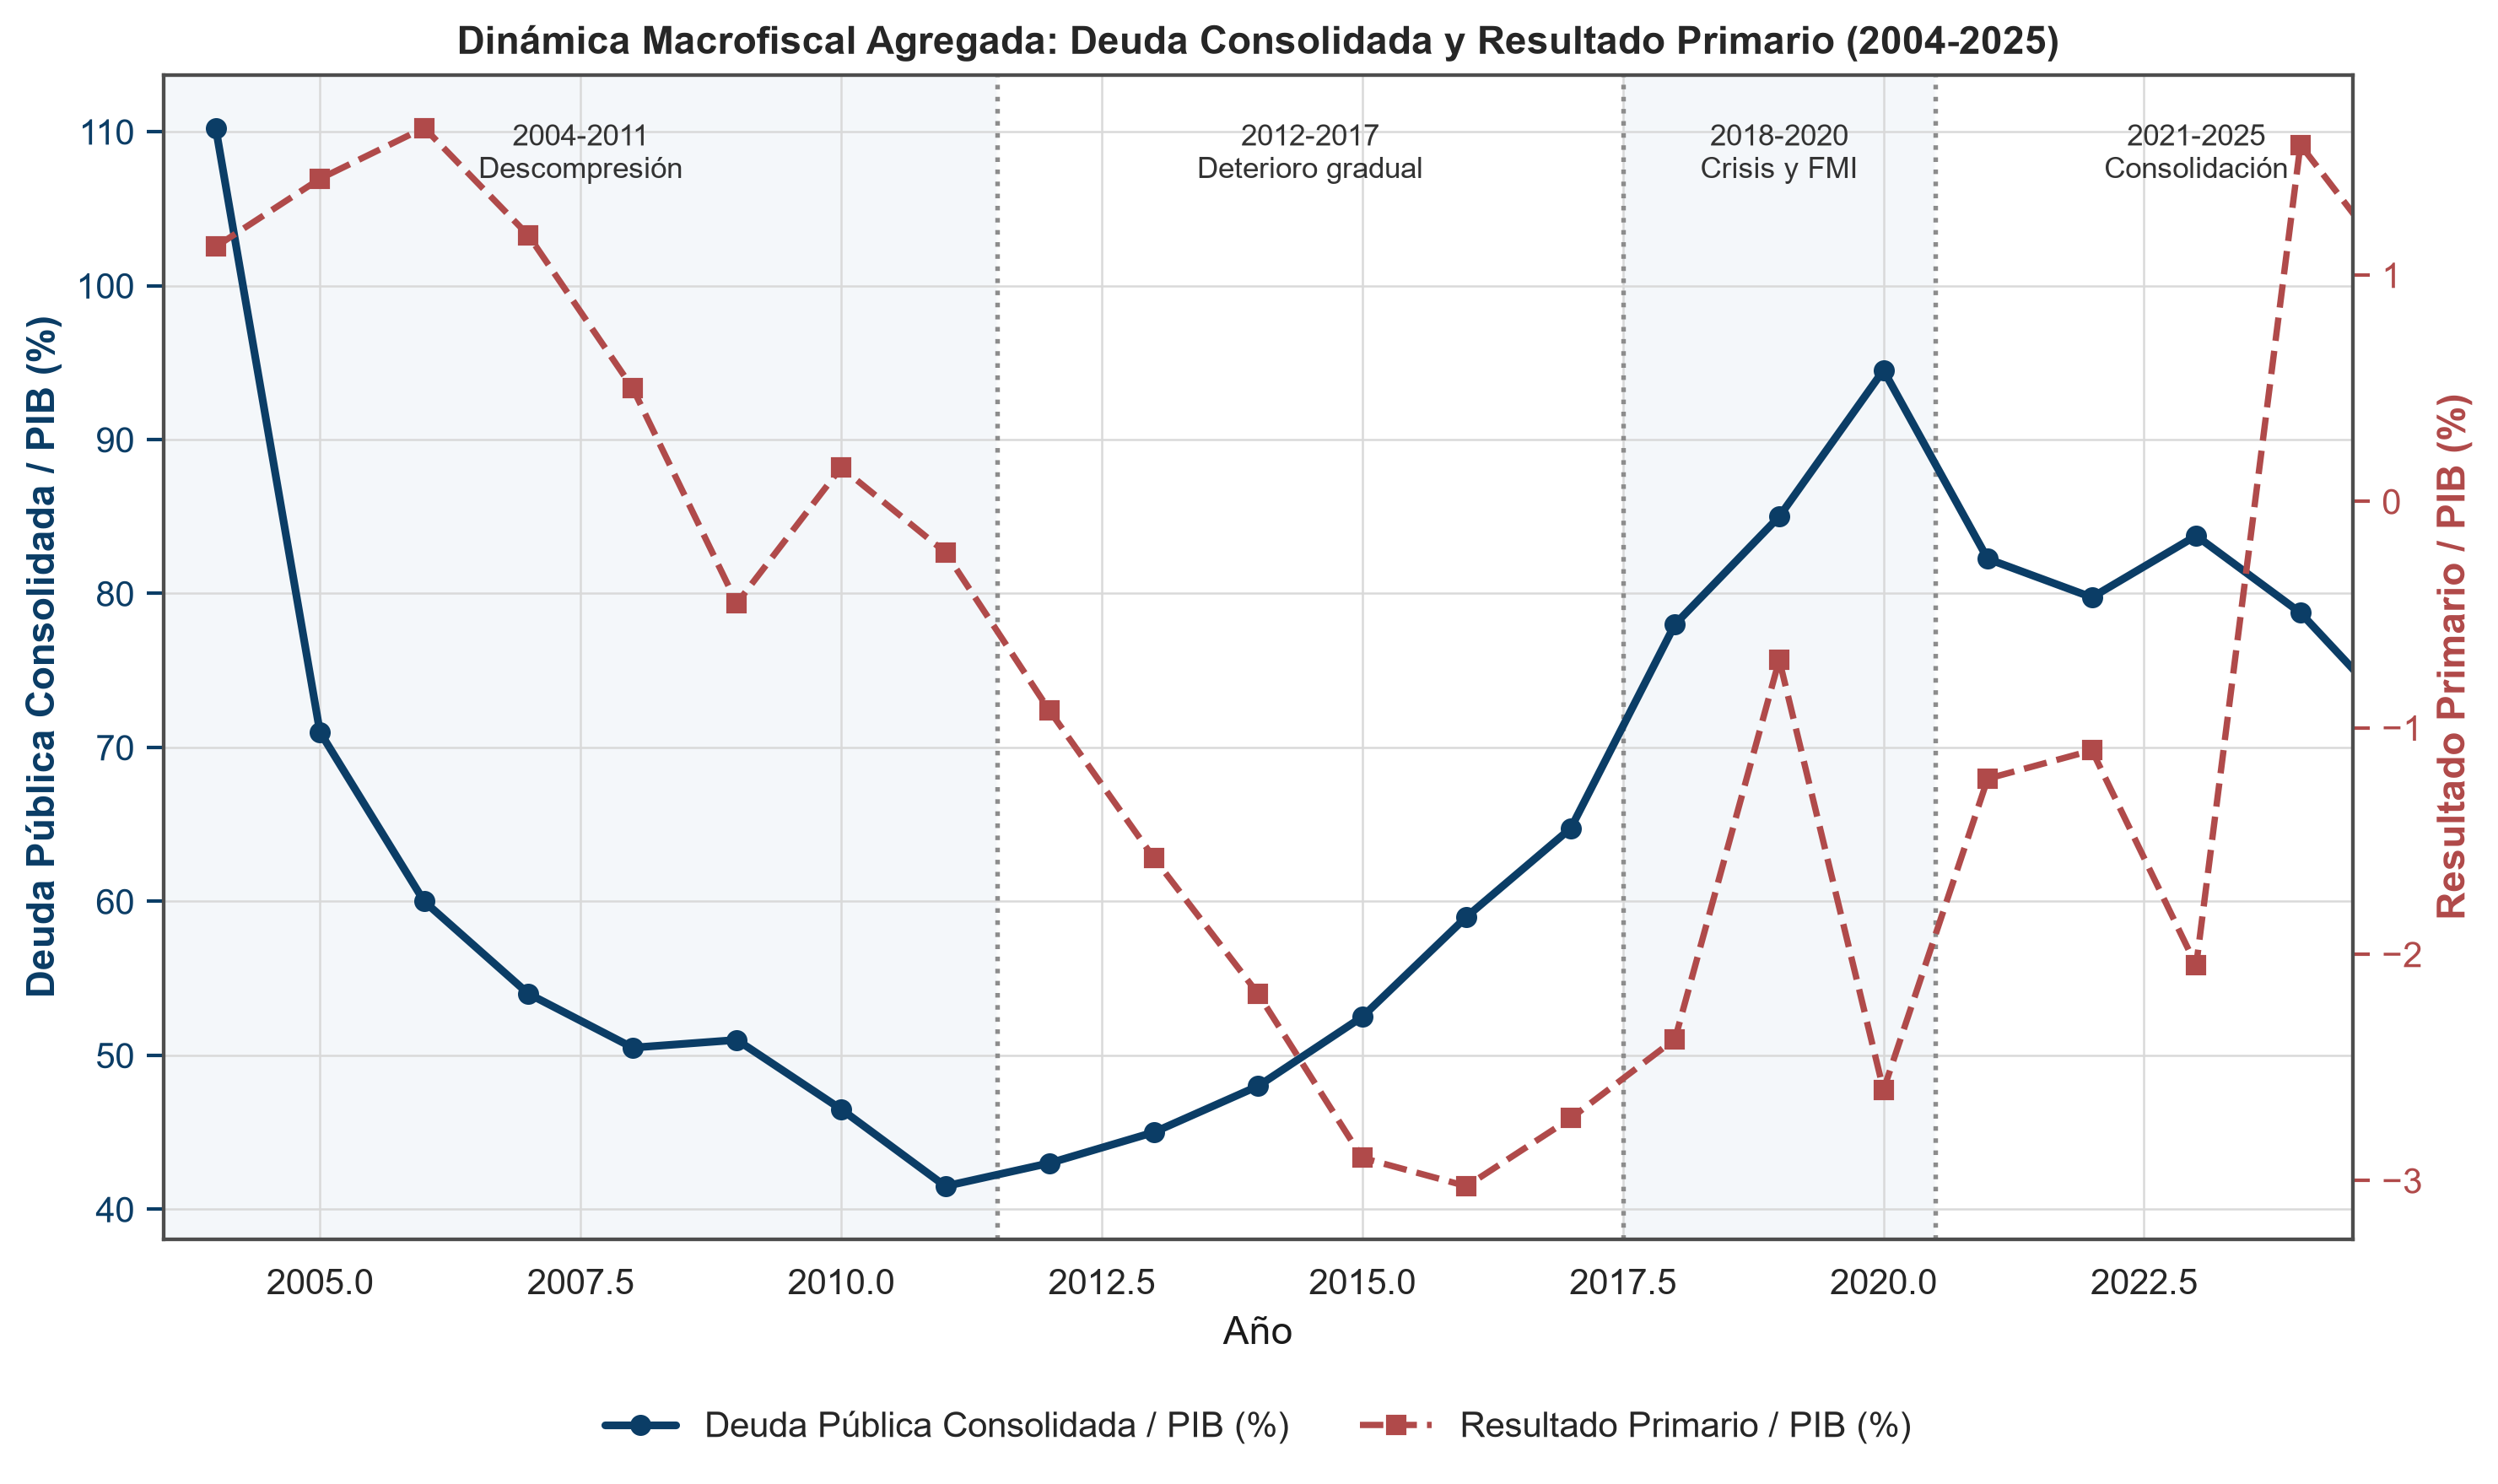
\includegraphics[width=0.95\textwidth]{fig5_1_deuda_resultado_primario.png}
\par\vspace{2mm}
{\footnotesize\textit{Nota.} Promedios anuales del panel trimestral, con ejes duales (deuda: eje izquierdo; resultado primario: eje derecho) y delimitación de los cuatro regímenes macrofiscales sucesivos. Elaboración propia en base a \texttt{dataset\_consolidado\_real.csv} (\texttt{codigo/graficos/generacion\_graficos\_tesis.py}).}
\end{figure}

La lectura revela cuatro regímenes sucesivos. Entre 2004 y 2011, la ratio de endeudamiento colapsa desde 110\% hasta un piso de 41.50\%, impulsada por la quita del canje de 2005 y por superávits primarios sostenidos (1.10\%--1.65\% del PIB) financiados por términos de intercambio favorables. Entre 2012 y 2017, el resultado primario se deteriora de manera continua hasta un déficit de 3.00\% del PIB en 2016, mientras la ratio de deuda recupera terreno moderadamente (de 43.00\% a 64.75\%). El tercer régimen, 2018--2020, es el más abrupto: la crisis cambiaria de 2018, el acuerdo \textit{stand-by} con el FMI (cuya ejecución fue objeto de una auditoría posterior de la Auditoría General de la Nación \citep{agn2023}) y la pandemia empujan la deuda hasta 94.50\% del PIB en apenas dos años. Finalmente, entre 2021 y 2025, el resultado primario retorna a terreno superavitario (1.58\% en 2024, 0.98\% en 2025) y la ratio de deuda desciende hasta 71.50\% del PIB.

Ninguno de estos cuatro regímenes se explica exclusivamente por el esfuerzo fiscal corriente: la descompresión 2004--2011 combina quita nominal, crecimiento del denominador y términos de intercambio favorables con auge de materias primas; el salto 2018--2020 combina devaluación real, prima de riesgo creciente y contracción del producto. Esta observación constituye la motivación empírica directa para instrumentar el riesgo soberano en el Capítulo \ref{ch:resultados}.

\section{Efecto Hoja de Balance: Tipo de Cambio Real y Variación de Deuda}
\label{sec:hoja_balance}

Como advierte la literatura sobre economías bimonetarias \citep{sanches2019}, cuando una porción sustancial del pasivo público está denominada en moneda extranjera, una devaluación del tipo de cambio real dispara mecánicamente el numerador de la ratio Deuda/PIB, independientemente del resultado primario contemporáneo. La Figura \ref{fig:hoja_balance} contrasta el nivel anual del TCRM con la variación interanual de la ratio de deuda.

\begin{figure}[H]
\centering
\caption{Efecto Hoja de Balance: Tipo de Cambio Real vs. Variación Anual de Deuda}
\label{fig:hoja_balance}
\begin{tikzpicture}
\begin{axis} [
    xlabel={Tipo de Cambio Real Multilateral (índice)},
    ylabel={Variación Interanual de la Ratio Deuda/PIB (p.p.)},
    xmin=1.10, xmax=2.45,
    ymin=-42, ymax=17,
    grid=both,
    grid style={dashed, gray!30},
    title style={font=\bfseries\small},
    label style={font=\small},
    tick label style={font=\scriptsize}
]
\addplot[only marks, mark=triangle*, color=teal, mark size=3pt] coordinates {
    (2.33,-39.2) (2.39,-11.0) (2.32,-6.0) (2.11,-3.5) (2.08,0.5) (1.88,-4.5)
    (1.76,-5.0) (1.51,1.5) (1.45,2.0) (1.53,3.0) (1.20,4.5) (1.36,6.5)
    (1.27,5.8) (1.58,13.2) (1.75,7.0) (1.70,9.5) (1.64,-12.2) (1.38,-2.5)
    (1.40,4.0) (1.37,-5.0) (1.29,-7.2)
};
\addplot[domain=1.15:2.4, red, thick] {-15.8*x + 24.71};
\end{axis}
\end{tikzpicture}
\par\vspace{2mm}
{\footnotesize\textit{Nota.} Impacto de las variaciones del tipo de cambio real sobre el stock de pasivos. Recta de ajuste MCO simple (referencial). Elaboración propia en base a \texttt{dataset\_consolidado\_real.csv} (BCRA, INDEC).}
\end{figure}

El primer punto (TCRM promedio 2005 $=2.33$, $\Delta d = -39.2$ p.p.) corresponde a la quita nominal del canje de deuda de 2005, no a un valor atípico de medición: se conserva en el gráfico por ser información genuina, y explica por sí solo buena parte de la pendiente negativa del ajuste MCO de nivel anual. Este resultado no debe confundirse con el mecanismo de hoja de balance propiamente dicho, que opera sobre \textit{variaciones} del tipo de cambio, no sobre su nivel. En términos de variaciones interperiódicas trimestrales, la correlación empírica entre la primera diferencia del TCRM ($\Delta TCRM_t$) y la variación de la ratio Deuda/PIB ($\Delta d_t$) alcanza $r=0.14$, positiva pero débil: consistente en signo con el mecanismo de hoja de balance, pero muy lejos de una relación determinística. Esta correlación es sensiblemente más débil que la calculada sobre el TCRM de contingencia utilizado hasta la Sección \ref{sec:auditoria_fallback} del Capítulo \ref{ch:metodologia} ($r=0.42$); la brecha ilustra cuánto podía distorsionar una relación bivariada simple el uso de una serie de contingencia suavizada en lugar de la serie real, y refuerza que la variación del endeudamiento obedece a una combinación de factores (resultado primario, crecimiento, tipo de cambio y ajustes stock-flujo), y no a un único indicador aislado.

\section{Protocolo de Estacionariedad y Pruebas de Raíz Unitaria}
\label{sec:estacionariedad}

Para evitar el riesgo de regresiones espurias, el protocolo evalúa el orden de integración de cada serie mediante dos contrastes complementarios: el test ADF (hipótesis nula: raíz unitaria) y el test KPSS (hipótesis nula: estacionariedad). La complementariedad de ambos, que testean hipótesis nulas opuestas, permite identificar con mayor robustez los casos ambiguos, especialmente relevantes en muestras de tamaño moderado como la sub-muestra de cobertura real aquí utilizada ($n=88$), necesaria para incluir al CER dentro de un panel comparable (Sección \ref{sec:empalme} del Capítulo \ref{ch:metodologia}).

\begin{table}[H]
\centering
\caption{\label{tab:estacionariedad} Pruebas de raíz unitaria e integración de las series (niveles y primeras diferencias).}
\resizebox{\textwidth}{!}{%
\begin{tabular}{lccccc}
\toprule
\textbf{Variable} & \textbf{ADF $p$ (nivel)} & \textbf{KPSS $p$ (nivel)} & \textbf{ADF $p$ (dif.)} & \textbf{KPSS $p$ (dif.)} & \textbf{Orden} \\
\midrule
Deuda / PIB & 0.113 & 0.041 & 0.000 & 0.035 & Ambiguo / I(1) \\
Result. Primario / PIB & 0.301 & 0.023 & 0.000 & 0.100 & I(1) \\
Brecha del Producto & 0.001 & 0.100 & 0.001 & 0.100 & I(0) \\
EMBI+ & 0.006 & 0.100 & 0.000 & 0.100 & I(0) \\
TCRM & 0.511 & 0.010 & 0.000 & 0.100 & I(1) \\
CER & 0.999 & 0.016 & 1.000 & 0.020 & Ambiguo / I(1) \\
\bottomrule
\end{tabular}%
}
\begin{flushleft}
\footnotesize \textit{Nota.} Elaboración propia. Test ADF bajo hipótesis nula de raíz unitaria; test KPSS bajo hipótesis nula de estacionariedad. p-valores reportados.
\end{flushleft}
\end{table}

Los resultados exhiben un panel de integración mixta, con implicancias metodológicas directas. La brecha del producto y el EMBI+ son estacionarias en niveles, I(0): oscilan en torno a una media constante, coherente con su naturaleza de variables cíclicas. El Resultado Primario y el TCRM son I(1): el ADF no rechaza la raíz unitaria en niveles mientras el KPSS rechaza estacionariedad; ambas se estabilizan tras la primera diferencia. Los casos de la Deuda/PIB y del CER producen un diagnóstico ambiguo, síntoma habitual de series estacionarias en torno a una tendencia con quiebre estructural (\textit{trend-stationary with a structural break}), que la Sección \ref{sec:zivot_andrews} somete a contraste formal.

Como evidencia visual complementaria, la Figura \ref{fig:acf_pacf} presenta los correlogramas ACF y PACF de las cuatro series núcleo. El decaimiento lento de la ACF del Resultado Primario y de la ratio Deuda/PIB, frente al corte abrupto tras el primer rezago de la Brecha del Producto y del EMBI+, ofrece una confirmación gráfica directa de la distinción entre series persistentes (I(1)) y de reversión rápida a la media (I(0)).

\begin{figure}[H]
\centering
\caption{Funciones de Autocorrelación Simple (ACF) y Parcial (PACF) de las Series Núcleo}
\label{fig:acf_pacf}
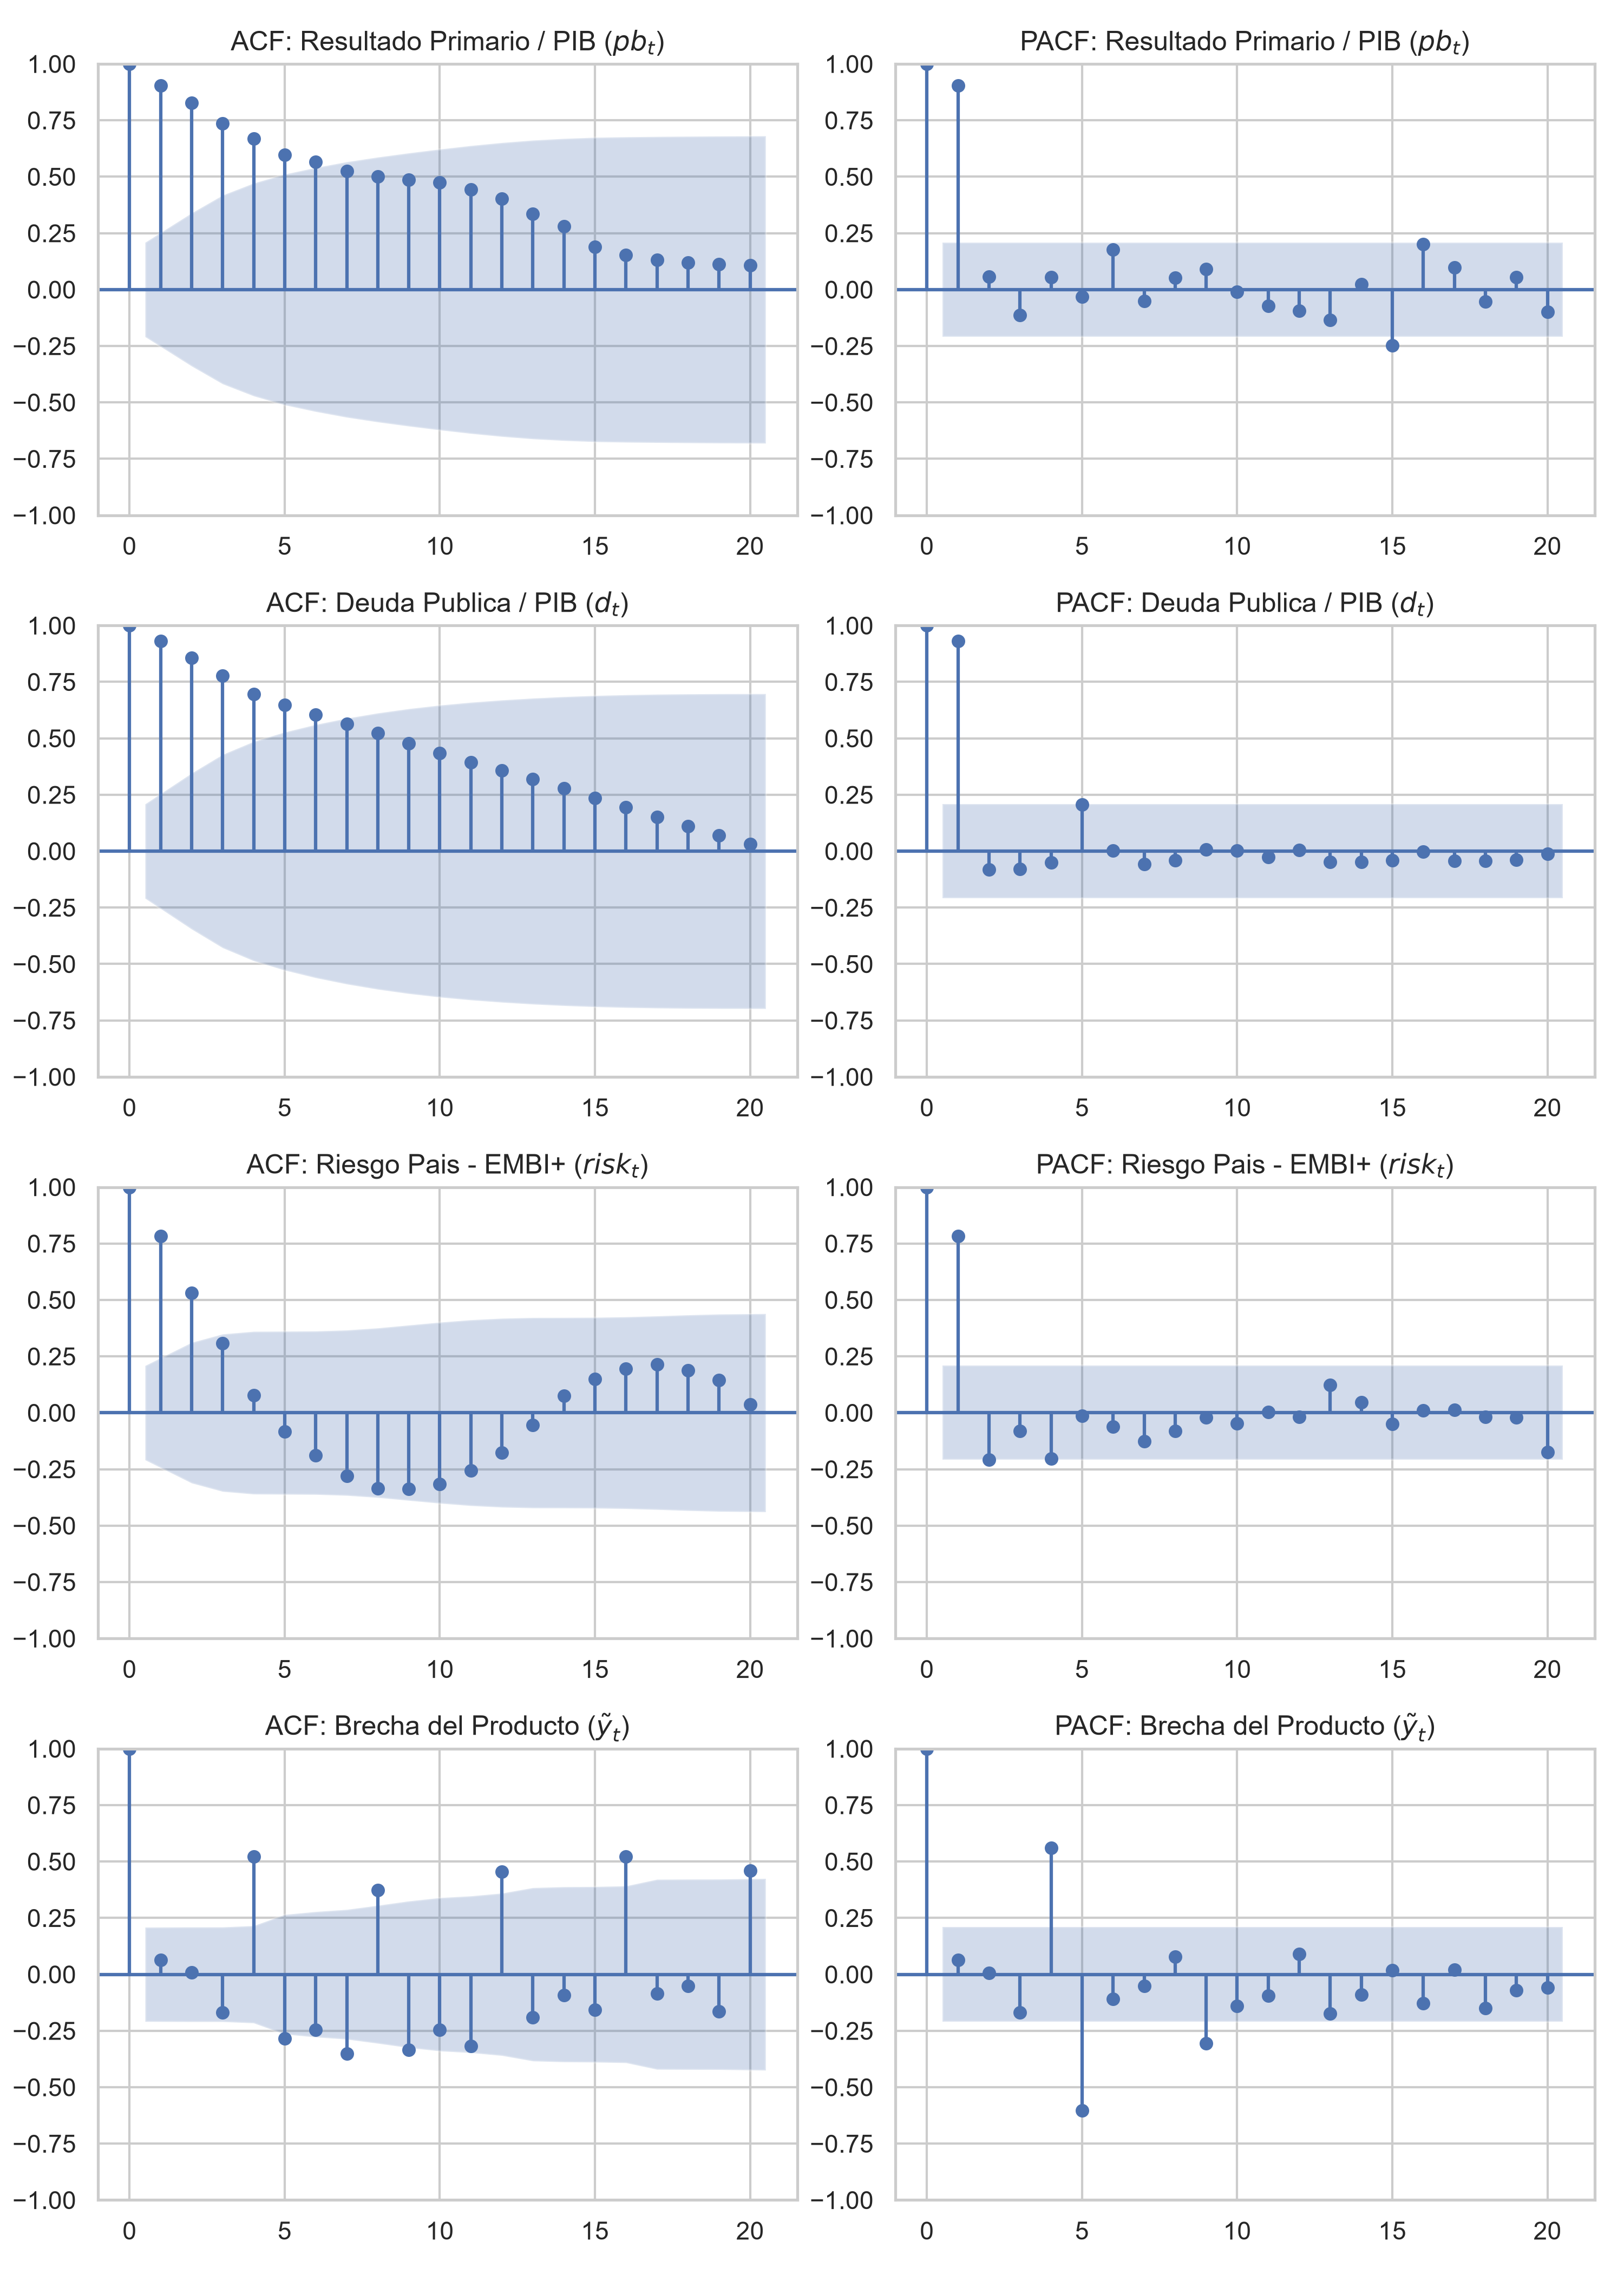
\includegraphics[width=0.85\textwidth]{figura_5_5_acf_pacf.png}
\par\vspace{2mm}
{\footnotesize\textit{Nota.} ACF (izquierda) y PACF (derecha, método Yule-Walker modificado) para 20 rezagos, con bandas de significatividad al 95\%. Elaboración propia en base a \texttt{dataset\_consolidado\_real.csv} (\texttt{codigo/modelos/fase7\_diagnosticos\_robustez.py}).}
\end{figure}

\subsection{Contraste de Zivot-Andrews con Quiebre Estructural Endógeno}
\label{sec:zivot_andrews}

A diferencia de los contrastes con quiebre exógeno (Chow, Perron), el algoritmo de Zivot-Andrews no requiere especificar \textit{a priori} la fecha de ruptura. El procedimiento itera sobre cada fecha candidata $T_B$ dentro de una ventana de recorte del 15\% en cada extremo, estimando para cada una la regresión MCO del Modelo C (quiebre simultáneo en intercepto y pendiente):
\[
\Delta d_t = c + \alpha\, d_{t-1} + \beta t + \theta\, DU_t(T_B) + \gamma\, DT_t(T_B) + \sum_{j=1}^{4} \phi_j \Delta d_{t-j} + \varepsilon_t
\]
donde $DU_t(T_B)=\mathbb{I}(t>T_B)$ y $DT_t(T_B)=(t-T_B)\cdot\mathbb{I}(t>T_B)$, y selecciona el $T_B$ que minimiza el estadístico $t$ asociado a $\alpha$. El rezago aumentado se fijó en $k=4$ trimestres.

Aplicado a la ratio Deuda/PIB sobre la ventana única (1996T1--2025T4, $n=120$), el algoritmo localiza el quiebre óptimo en 2004T2. El estadístico $t$ obtenido ($-4.50$) tampoco rechaza la hipótesis nula de raíz unitaria bajo ningún umbral crítico asintótico del Modelo C ($-5.58$ al 1\%, $-5.07$ al 5\%, $-4.83$ al 10\%), aunque se acerca sensiblemente más al crítico del 10\% que el resultado obtenido en una estimación previa sobre la sub-muestra de 88 observaciones ($t=-2.83$, quiebre en 2018T2). La ratio de deuda argentina se comporta, en consecuencia, como una serie genuinamente integrada de orden uno incluso permitiendo el quiebre más favorable a la alternativa de estacionariedad dentro de los treinta años de muestra. La restricción de un único quiebre es, además, insuficiente para una serie atravesada por múltiples reestructuraciones (2005, 2010, 2020) y episodios de interrupción repentina de capitales (\textit{sudden stop}, 2018), a los que ahora se suma la propia crisis de 2001--2002 dentro de la ventana: la Sección \ref{sec:quiebres_estructurales} extiende el análisis a un marco de quiebres múltiples, y la implicancia metodológica inmediata motiva la batería de pruebas de Johansen y la estimación DOLS desarrolladas en el Capítulo \ref{ch:resultados}.

\subsection{Deuda Consolidada: Incorporación de los Pasivos Remunerados del BCRA}
\label{sec:deuda_consolidada}

La delimitación del Capítulo \ref{ch:metodologia} circunscribe $d_t$ al SPNF, excluyendo la absorción monetaria del BCRA: LEBAC/NOBAC (2002--2018), LELIQ/NOTALIQ (2018--2024) y la posición neta de pases. El devengamiento de intereses de estos instrumentos constituye un déficit cuasi-fiscal ausente del resultado primario del Tesoro, estimado en el orden del 9\%--10\% del PIB en su pico reciente. Como extensión de robustez, se construyó una serie de pasivos remunerados del BCRA a partir de las series oficiales v4.0 del BCRA (idVariable 1258, 1260 y 1261) y del PIB nominal trimestral de INDEC, sin neteo adicional entre ambos stocks.

La brecha promedio entre ambas definiciones es de 5.5 puntos porcentuales del PIB, con un pico de 10.6\% en el primer trimestre de 2018 y una caída a valores prácticamente nulos desde mediados de 2024, cuando el Tesoro asumió el rol de esterilizador monetario mediante Letras Fiscales de Liquidez (LEFI). La Figura \ref{fig:deuda_consolidada} contrasta ambas series.

\begin{figure}[H]
\centering
\caption{Deuda Pública: SPNF vs. Consolidada con Pasivos Remunerados del BCRA}
\label{fig:deuda_consolidada}
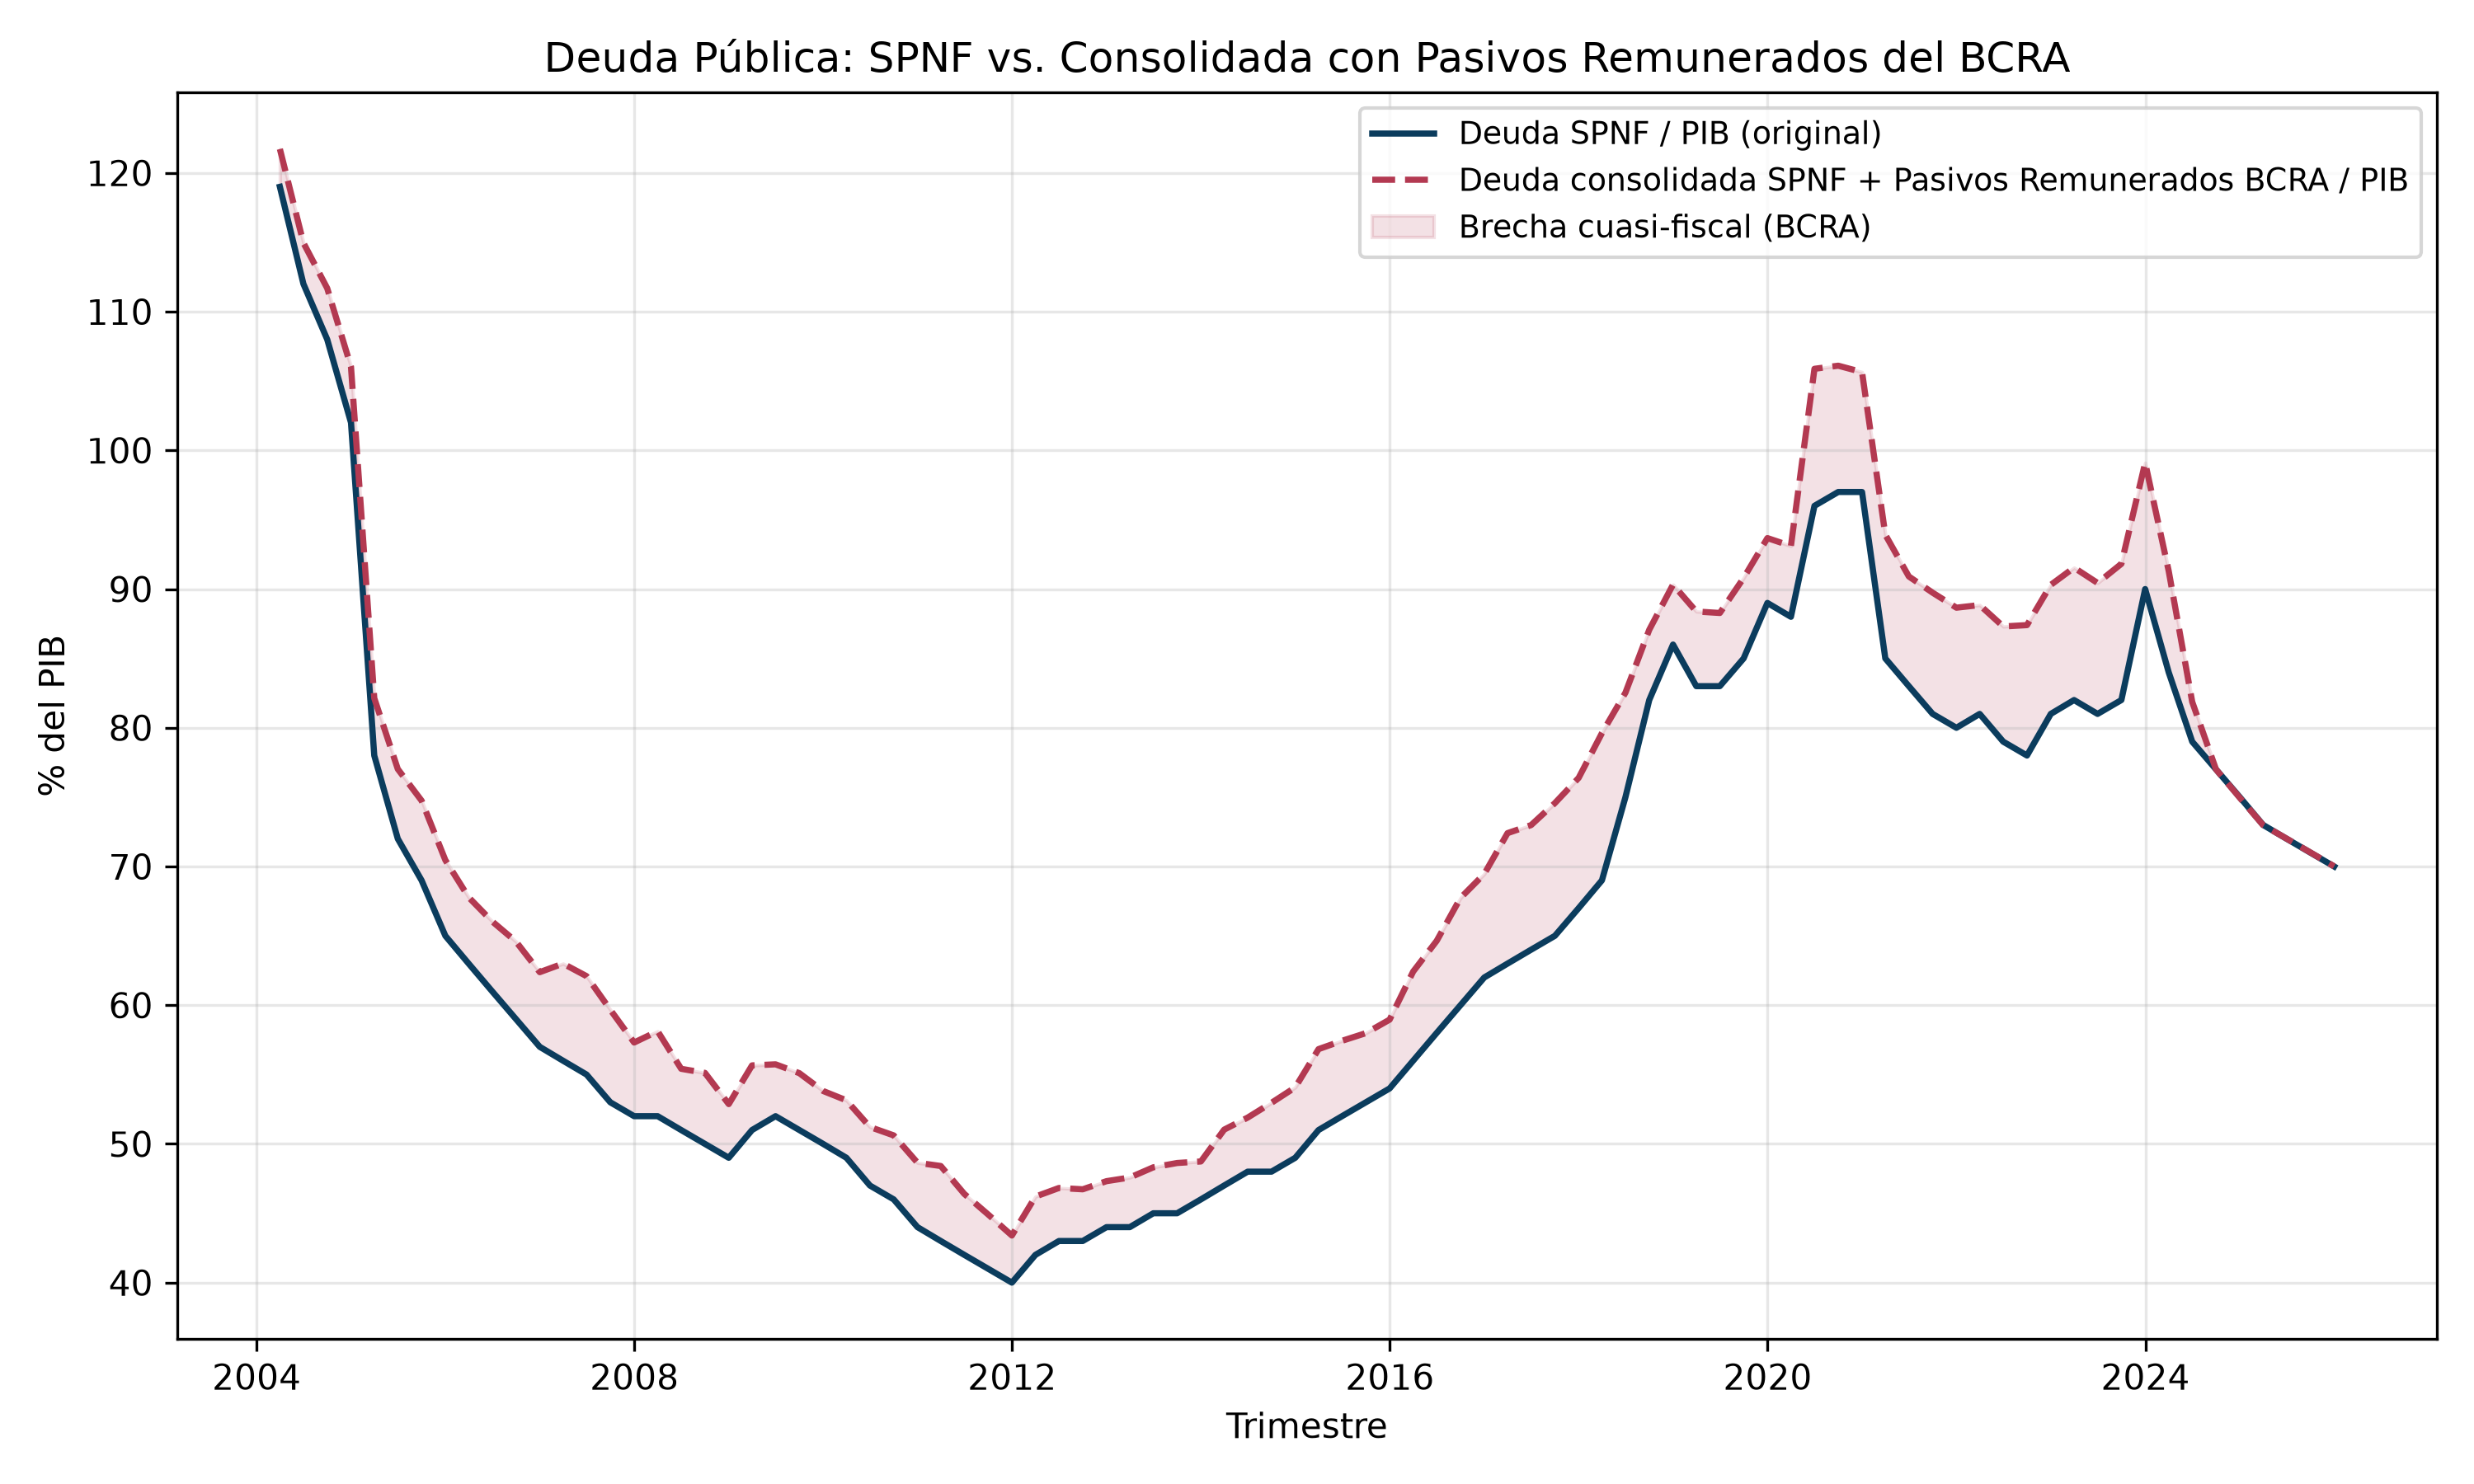
\includegraphics[width=0.95\textwidth]{figura_8_1_deuda_consolidada.png}
\par\vspace{2mm}
{\footnotesize\textit{Nota.} Elaboración propia en base a series oficiales BCRA v4.0 y PIB nominal INDEC (\texttt{codigo/ingesta\_datos/ingesta\_bcra\_pasivos.py}, \texttt{codigo/modelos/fase8\_deuda\_consolidada.py}).}
\end{figure}

La serie consolidada conserva el orden de integración de la serie SPNF (ADF no rechaza en niveles, $p=0.169$; rechaza en primera diferencia, $p<0.001$; KPSS rechaza estacionariedad en niveles, $p=0.038$), coherente con I(1). La Sección \ref{sec:quiebres_estructurales} evalúa si la cronología de quiebres estructurales se modifica al incorporar esta capa cuasi-fiscal.

\subsection{Quiebres Estructurales Múltiples de Bai-Perron}
\label{sec:quiebres_estructurales}

El test de Zivot-Andrews impone la restricción de un único quiebre, insuficiente para una serie atravesada por las reestructuraciones soberanas de 2005, 2010 y 2020 y los episodios de \textit{sudden stop}. \textcite{bai2003} resuelven esta limitación estimando de manera consistente el número y la ubicación de quiebres múltiples sin conocimiento \textit{a priori} de sus fechas, mediante programación dinámica sobre la suma de cuadrados residuales de las particiones factibles, con selección del número de quiebres por el criterio BIC \citep{yao1988}.

El criterio BIC selecciona $m^*=3$ quiebres para la deuda SPNF sobre la ventana única completa (1996T1--2025T4, $n=120$): 2001T3, 2006T1 y 2017T3. Las medias estimadas por segmento son 34.68\% (1996T1--2001T3, $n=23$), 106.85\% (2001T4--2006T1, $n=18$), 50.72\% (2006T2--2017T3, $n=46$) y 81.24\% (2017T4--2025T4, $n=33$) del PIB: al incorporar el tramo 1996--2003, el algoritmo detecta por primera vez el quiebre de la crisis de 2001, invisible para una ventana que arrancara en 2004. Para la deuda consolidada con pasivos del BCRA, cuya cobertura permanece acotada a la sub-muestra de fuente primaria real (2004T1--2025T4, $n=88$, Sección \ref{sec:deuda_consolidada}) por no existir una serie de pasivos remunerados del BCRA verificable antes de 2004, el criterio selecciona $m^*=2$ quiebres en 2007T2 y 2016T4, con medias de 81.8\%, 53.5\% y 86.4\%, una cronología distinta a la de la deuda SPNF sola, coherente con que el peso cuasi-fiscal del BCRA introduce su propia dinámica de régimen.

\begin{figure}[H]
\centering
\caption{Quiebres Estructurales Múltiples de Bai-Perron (Selección por BIC)}
\label{fig:bai_perron}
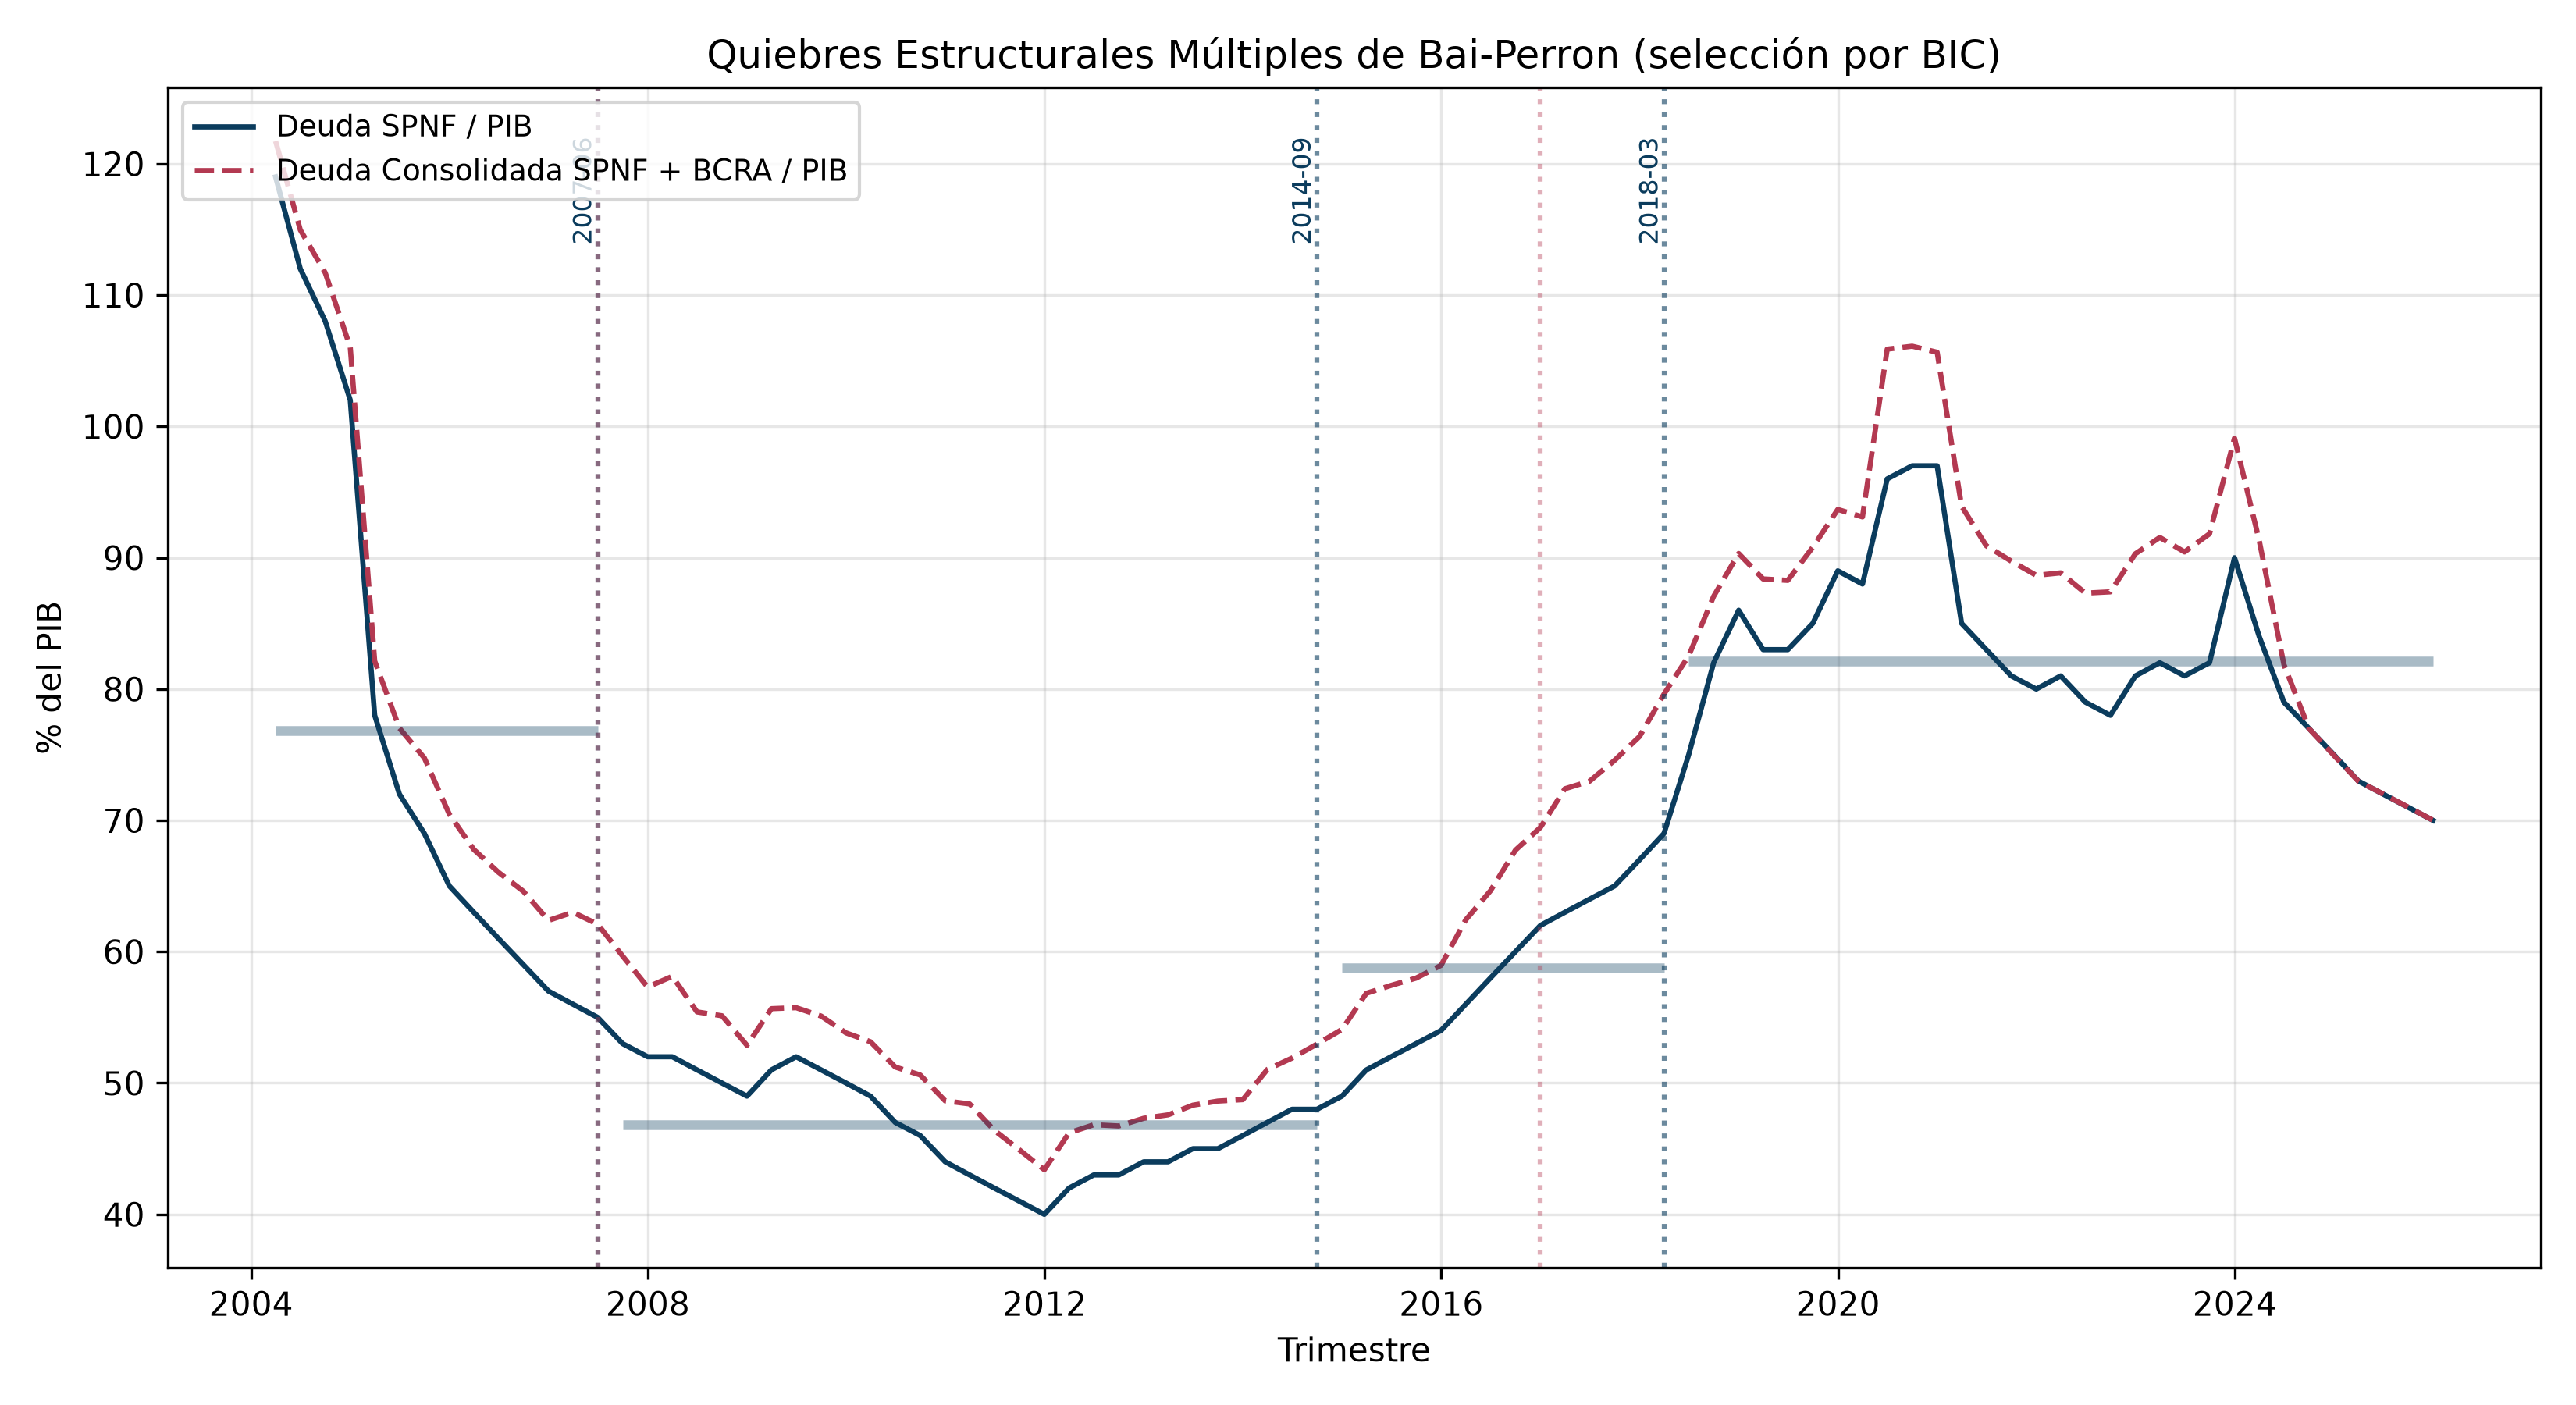
\includegraphics[width=0.95\textwidth]{figura_9_1_bai_perron.png}
\par\vspace{2mm}
{\footnotesize\textit{Nota.} Deuda SPNF vs. deuda consolidada SPNF+BCRA, con quiebres óptimos de Bai-Perron ($m^*=3$ y $m^*=2$ respectivamente) y medias de segmento superpuestas. Elaboración propia en base a \texttt{dataset\_consolidado\_real.csv} (\texttt{codigo/modelos/fase9\_bai\_perron.py}).}
\end{figure}

Como evidencia exploratoria complementaria, se aplicó sobre el Resultado Primario un algoritmo de detección de quiebres por programación dinámica de costo $L_2$ (paquete \texttt{ruptures} \citep{truong2020}), fijando cuatro particiones para permitir una lectura comparable con los cuatro regímenes macrofiscales de la Figura \ref{fig:dinamica_stocks_flujos}.

\begin{figure}[H]
\centering
\caption{Cronología de Quiebres Estructurales Múltiples en el Resultado Primario}
\label{fig:quiebres_timeline}
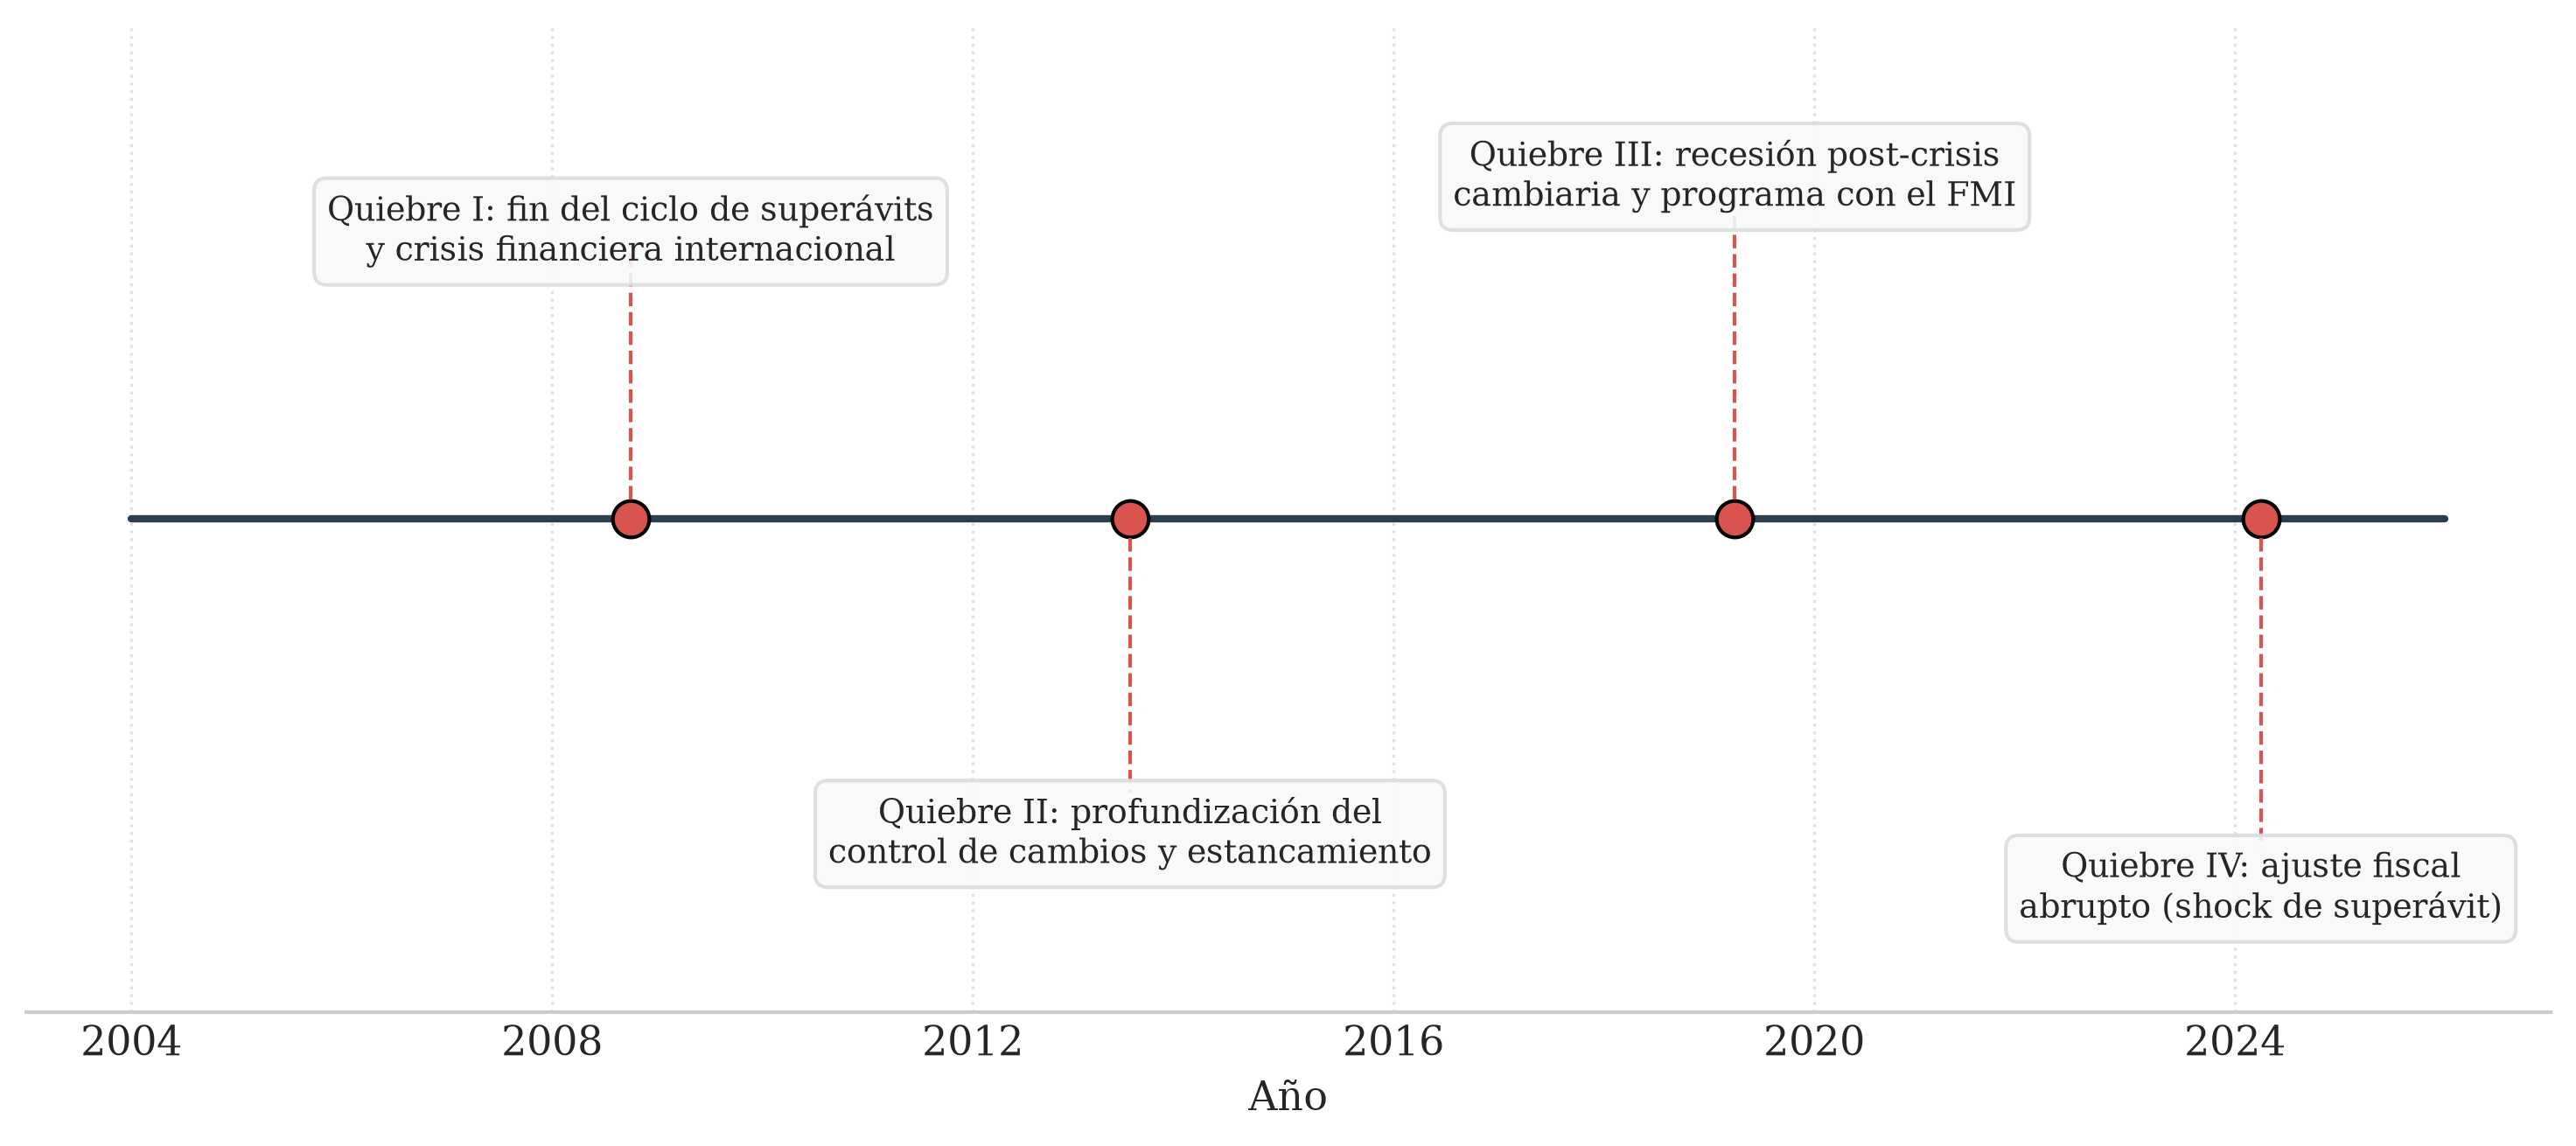
\includegraphics[width=0.95\textwidth]{figura_5_4_quiebres_timeline.png}
\par\vspace{2mm}
{\footnotesize\textit{Nota.} Quiebres detectados mediante programación dinámica (costo $L_2$, \texttt{ruptures}), en el espíritu del enfoque de partición óptima de \textcite{bai2003} (Sección \ref{sec:zivot_andrews}). Elaboración propia en base a \texttt{dataset\_consolidado\_real.csv} (\texttt{codigo/graficos/generacion\_cronologia\_quiebres.py}).}
\end{figure}

Los cuatro quiebres detectados (2008T3, 2013T2, 2019T1 y 2024T1) se aproximan a los límites de los cuatro regímenes macrofiscales identificados en la Sección anterior, con desfases de entre uno y cuatro trimestres. Esta coincidencia aproximada confirma que los regímenes macrofiscales identificados no son arbitrarios, aunque no coinciden mecánicamente con el punto de quiebre estadísticamente óptimo de la serie de resultado primario aislada.

\section{Matriz de Correlaciones Bivariadas y Diagnóstico de Multicolinealidad}
\label{sec:correlaciones_vif}

La evaluación de las correlaciones bivariadas arroja tres resultados relevantes para el diseño de la estrategia de instrumentación del Capítulo \ref{ch:resultados}. El VIX y el EMBI+ exhiben una correlación positiva pero prácticamente nula ($r=0.08$) en nivel contemporáneo: sobre la serie real de EMBI+, el canal de fuga hacia la calidad (vuelo hacia la calidad) de la literatura de finanzas internacionales no se manifiesta en la correlación simple de niveles, a diferencia de lo que sugería la serie de contingencia usada hasta la Sección \ref{sec:auditoria_fallback} del Capítulo \ref{ch:metodologia} ($r=0.33$); lo que no descarta el canal sino que exige una especificación menos ingenua (dinámica, no contemporánea) para detectarlo, motivo adicional para instrumentar el EMBI+ con el VIX en la Etapa 4 (Capítulo \ref{ch:resultados}) en lugar de inferir la relación de una correlación de nivel. La brecha del producto y el resultado primario muestran una correlación prácticamente nula ($r=0.07$). Esto no debe leerse como evidencia de una política contracíclica ejemplar: advierte, en cambio, que la correlación contemporánea simple no captura relaciones rezagadas, no lineales, ni mediadas por terceras variables, que la estimación multivariada del Capítulo \ref{ch:resultados} sí controla. Finalmente, la correlación entre la primera diferencia del TCRM y de la ratio de deuda ($r=0.14$, Sección \ref{sec:hoja_balance}) es positiva pero débil, la más débil de las tres pese a ser, sobre la serie de contingencia previa, la que se reportaba como más robusta.

La correlación bivariada, no obstante, no permite descartar dependencias lineales entre tres o más regresores simultáneamente. Se complementa por ello con los factores de inflación de la varianza (VIF) y el número de condición de la matriz de regresores estandarizados, calculados sobre las dos especificaciones relevantes para el Capítulo \ref{ch:resultados} y reportados en la Tabla \ref{tab:vif}.

\begin{table}[H]
\centering
\caption{\label{tab:vif} Diagnóstico de Multicolinealidad: Factores de Inflación de la Varianza y Número de Condición.}
\begin{tabular}{llrr}
\toprule
\textbf{Especificación} & \textbf{Regresor} & \textbf{VIF} & \textbf{Núm. de condición} \\
\midrule
\multirow{2}{*}{Núcleo de Bohn (DOLS)} & $d_{t-1}$ & 1.020 & \multirow{2}{*}{1.151} \\
 & Brecha del producto ($\tilde{y}_t$) & 1.020 & \\
\midrule
\multirow{4}{*}{Ampliada (Bohn + EMBI+ + TCRM)} & $d_{t-1}$ & 1.869 & \multirow{4}{*}{2.381} \\
 & Brecha del producto ($\tilde{y}_t$) & 1.025 & \\
 & EMBI+ & 1.910 & \\
 & TCRM & 1.046 & \\
\bottomrule
\end{tabular}
\begin{flushleft}
\footnotesize \textit{Nota.} $n=87$ en ambas especificaciones. Umbrales convencionales de alerta: $VIF>10$ y número de condición $>30$. El número de condición se computa sobre los regresores estandarizados, excluyendo la constante. Elaboración propia en base a \texttt{dataset\_consolidado\_real.csv} (\texttt{codigo/modelos/fase12\_diagnosticos\_complementarios.py}).
\end{flushleft}
\end{table}

Ninguna de las dos especificaciones exhibe multicolinealidad problemática. En el núcleo de Bohn, la especificación efectivamente estimada por DOLS, los dos regresores son prácticamente ortogonales ($VIF=1.02$, número de condición $=1.15$). En la especificación ampliada, con la serie real de TCRM y EMBI+, los cuatro regresores permanecen igualmente cerca de la ortogonalidad ($VIF$ entre $1.02$ y $1.91$, número de condición $=2.38$), muy por debajo tanto del umbral convencional de $10$ como del número de condición de $30$. Sobre la serie de contingencia utilizada hasta la Sección \ref{sec:auditoria_fallback} del Capítulo \ref{ch:metodologia}, el VIF de $d_{t-1}$ y de TCRM llegaba a $3.82$ y $3.69$ respectivamente (número de condición $3.84$): también por debajo de los umbrales de alerta, pero sensiblemente más alto que con la serie real, un indicio adicional de que la serie de contingencia introducía una colinealidad artificial con la trayectoria de la deuda que la serie real no reproduce. La imprecisión de los coeficientes reportada en el Capítulo \ref{ch:resultados} no es, en ningún caso, atribuible a colinealidad entre regresores.

\section{Dispersión Empírica y la Hipótesis de Fatiga Fiscal}

Como aproximación descriptiva preliminar a la hipótesis central de esta tesis ($H_{1a}$), la Figura \ref{fig:scatter_fatiga} cruza el nivel de deuda heredado ($d_{t-1}$) con el esfuerzo fiscal contemporáneo ($pb_t$) para el panel trimestral completo.

\begin{figure}[H]
\centering
\caption{Dispersión Empírica: Esfuerzo Primario vs. Endeudamiento Heredado}
\label{fig:scatter_fatiga}
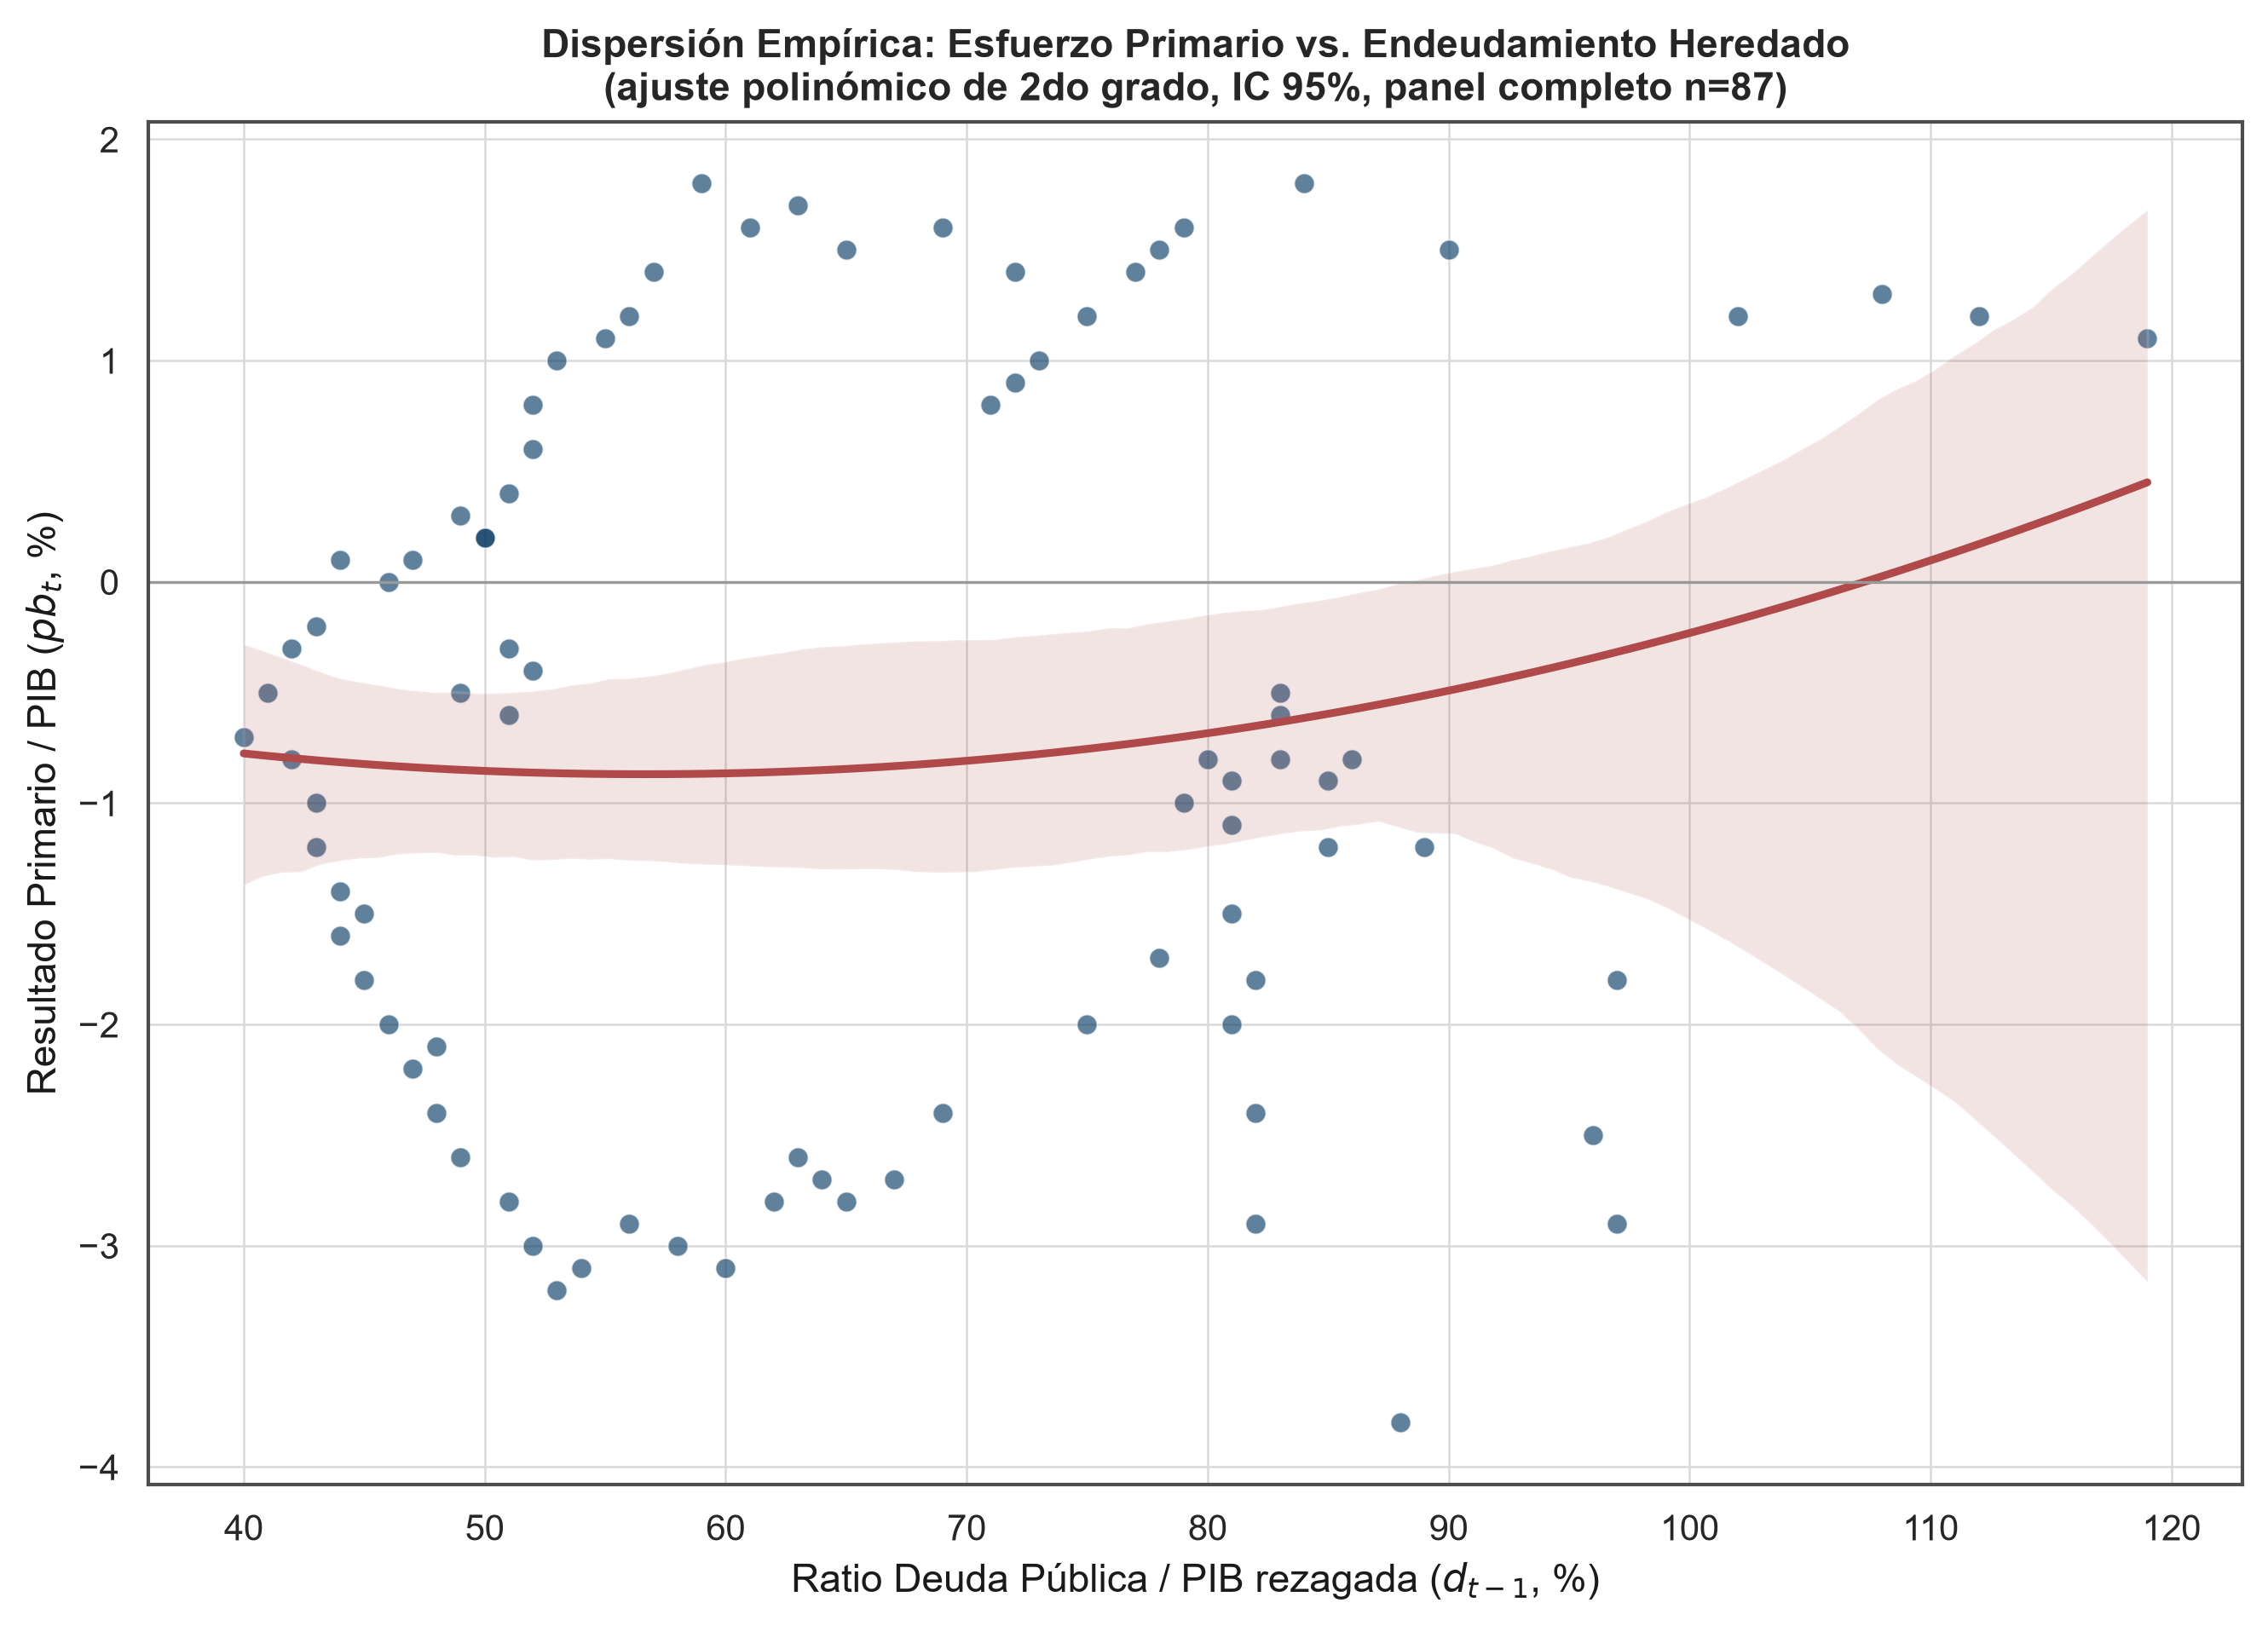
\includegraphics[width=0.85\textwidth]{fig5_3_dispersion_fatiga_fiscal.png}
\par\vspace{2mm}
{\footnotesize\textit{Nota.} Dispersión empírica trimestral completa (87 pares $(d_{t-1}, pb_t)$), con ajuste polinómico local de segundo grado e intervalo de confianza del 95\% sombreado. Elaboración propia en base a \texttt{dataset\_consolidado\_real.csv} (\texttt{codigo/graficos/generacion\_graficos\_tesis.py}).}
\end{figure}

La nube de puntos sugiere, a simple vista, un patrón compatible con la hipótesis de fatiga fiscal: los superávits más altos (en torno a 1.00\%--1.60\% del PIB) se concentran en la región de deuda baja o moderada (40.00\%--70.00\%), mientras que la región de deuda elevada (80.00\%--120.00\%) exhibe mayoritariamente resultados deficitarios, con dos excepciones recientes (2024--2025) que reintroducen superávits modestos bajo un nivel de deuda todavía relativamente alto (79.00\% y 73.00\%). Es necesario, no obstante, evitar inferir un umbral en esta etapa descriptiva bivariada: la dispersión no controla por la brecha del producto, el riesgo soberano contemporáneo ni la dinámica temporal de la serie, todos ellos factores que la especificación de umbral formal de \citet{hansen1999} incorpora explícitamente en el Capítulo \ref{ch:resultados}. Como se mostrará allí, cuando estos controles se introducen, la evidencia estadística del quiebre sugerido visualmente pierde buena parte de su fuerza aparente en la especificación de nivel, aunque una especificación alternativa formalmente más apropiada la recupera (Sección \ref{sec:robustez_hansen_dpb}).

\section{Limitaciones de la Muestra y Advertencias de Inferencia}
\label{sec:limitaciones_muestra}

Los resultados presentados en este capítulo, y los que se desarrollarán en los Capítulos \ref{ch:resultados} y \ref{ch:discusion}, deben interpretarse a la luz de las limitaciones inherentes a la muestra. Las 120 observaciones trimestrales (1996T1--2025T4) constituyen la ventana muestral única de esta investigación (Sección \ref{sec:matriz_operacional} del Capítulo \ref{ch:metodologia}), de las cuales 88 (2004T1--2025T4) corresponden a la sub-muestra de cobertura 100\,\% real, sin tramo empalmado. Esta longitud muestral, adecuada para series de tiempo de un único país en condiciones de estacionariedad, limita la potencia estadística de pruebas como el umbral de Hansen y la cointegración de Johansen, especialmente en presencia de quiebres estructurales frecuentes.

El contexto de alta volatilidad estructural y regímenes de política cambiante, documentado en la cronología de Bai-Perron (Sección \ref{sec:quiebres_estructurales}), agrava esta limitación: cuando la variable de umbral (EMBI+, $\sigma=1573.84$ pb sobre la ventana única, Tabla \ref{tab:descriptivos_ampliado}) y la dependiente (resultado primario, $\sigma=1.73$ pp del PIB) están ambas sometidas a perturbaciones de magnitud comparable a la señal buscada, la relación señal-ruido se vuelve desfavorable para la identificación de quiebres discretos. Los tests de robustez implementados (subperíodos, especificaciones alternativas) confirman la fragilidad de inferencias fuertes sobre la significatividad estadística de los coeficientes individuales, lo que refuerza la necesidad de cautela en las proyecciones y de priorizar la consistencia del diagnóstico cualitativo sobre la precisión puntual de los estimadores.

La ventana única de 120 observaciones (Sección \ref{sec:ventana_ampliada}), que sostiene la totalidad del protocolo econométrico del Capítulo \ref{ch:resultados}, no releva de esta cautela: la desplaza a un terreno más nítido y, a la vez, más preocupante. El contraste de Johansen sobre la ventana 1996--2025 no rechaza la ausencia de cointegración para $r=0$ (traza $=45.18$ frente al valor crítico al 95\% de $47.85$), y el resultado se sostiene al variar el año de inicio de la muestra: la verificación sobre 1997--2025 ($n=116$, sin el empalme aproximado del TCRM de 1996) arroja una traza de $45.46$, prácticamente idéntica y también por debajo de ese mismo crítico. A diferencia de la ventana 1999--2025, que rechazaba $r=0$ en un punto de inicio de la muestra pero no en el otro, la ventana 1996--2025 no rechaza $r=0$ en ninguno de los dos puntos de inicio probados (Capítulo \ref{ch:resultados}): la ambigüedad sobre la existencia de una relación de cointegración estable no se reduce al ampliar la muestra, sino que se vuelve más marcada. Se impone $r=1$ por el mismo criterio teórico que ya empleaba la tesis, documentando explícitamente que esa imposición queda ahora menos respaldada por la evidencia estadística que antes.

Para abordar formalmente esta tensión entre longitud muestral y homogeneidad institucional, el Capítulo \ref{ch:resultados} (Sección \ref{sec:spread_historico_1983_2025}) desarrolla una extensión complementaria de ultra-largo plazo que reconstruye y empalma el spread soberano para los 42 años completos de democracia ininterrumpida ($1983\text{T4}$--$2025\text{T4}$, $n=169$), contrastando si los umbrales de fatiga fiscal identificados en la muestra central constituyen regularidades estructurales o artefactos circunscritos a las últimas dos décadas.


\chapter{Desarrollo Empírico y Resultados}
\label{ch:resultados}

Este capítulo contrasta empíricamente las hipótesis planteadas en el Capítulo \ref{ch:introduccion} mediante econometría de series de tiempo. El paso desde el análisis descriptivo del Capítulo \ref{ch:descriptivo} hacia la estimación econométrica permite evaluar los determinantes de la Función de Reacción Fiscal argentina sobre la ventana muestral única (1996--2025, $n=120$, treinta años exactos): DF-GLS, Johansen, VECM, DOLS, IV-2SLS, Hansen, Bai-Perron, el SVAR restringido y el Threshold VECM se estiman todos sobre esta misma ventana (Secciones \ref{sec:dfgls}--\ref{sec:tvecm_resultados}), con el VECM, el SVAR restringido y el Threshold VECM como técnica de referencia para la Función de Reacción Fiscal y el protocolo de no linealidad, en reemplazo de DOLS, a pedido del director de tesis (Secciones \ref{sec:vecm} y \ref{sec:svar_metodologia} del Capítulo \ref{ch:metodologia}). La evidencia recogida es mayormente débil o estadísticamente no concluyente: la regla de reacción fiscal lineal de Bohn no opera de forma estable bajo ninguna de las técnicas aplicadas. Dicha inoperancia estadística constituye el hallazgo central del capítulo y se analiza en profundidad en el Capítulo \ref{ch:discusion}, junto con la evidencia de un régimen crítico de riesgo soberano que el modelo de umbral de Hansen no confirma como fatiga fiscal en su especificación en niveles, sino como el patrón inverso (Sección \ref{sec:hansen}). La descomposición de varianza del SVAR restringido, por su parte, cambia de manera sustantiva respecto de lo que sostenía una estimación previa sobre una ventana más corta (Sección \ref{sec:svar_resultados}), y esa reversión se discute con el mismo criterio de transparencia que el resto del capítulo.

\section{Contrastes Adicionales de Raíz Unitaria (DF-GLS)}
\label{sec:dfgls}

La Sección \ref{sec:estacionariedad} del Capítulo \ref{ch:descriptivo} ya avanzó un diagnóstico de integración basado en los contrastes complementarios de ADF y KPSS. Para robustecerlo se aplica adicionalmente el test de raíz unitaria \textit{Dickey-Fuller Generalized Least Squares} (DF-GLS) de \textcite{elliott1996}, que remueve la tendencia determinística mediante mínimos cuadrados generalizados antes de estimar la regresión aumentada, logrando una potencia estadística sustancialmente mayor que el ADF convencional en muestras acotadas como la presente ($n=120$).

\begin{table}[H]
\centering
\caption{\label{tab:dfgls} Resultados del Test de Raíz Unitaria DF-GLS (Elliott-Rothenberg-Stock, 1996), Ventana Única (1996--2025).}
\resizebox{\textwidth}{!}{%
\begin{tabular}{lrrrrl}
\toprule
\textbf{Variable} & \textbf{Estad. (nivel)} & \textbf{Crít. 5\% (nivel)} & \textbf{Estad. (1.\ dif.)} & \textbf{Crít. 5\% (1.\ dif.)} & \textbf{Conclusión} \\
\midrule
$pb_t$ & -1.30 & -3.01 & -5.98 & -2.12 & I(1) \\
$d_t$ & -2.65 & -3.01 & -4.07 & -2.12 & I(1) \\
EMBI+ ($risk_t$) & -2.30 & -3.01 & -9.16 & -2.11 & I(1) \\
$\tilde{y}_t$ & -3.46 & -3.02 & -4.93 & -2.12 & I(0) \\
\bottomrule
\end{tabular}%
}
\begin{flushleft}
\footnotesize \textit{Nota.} Elaboración propia (\texttt{codigo/modelos/fase1\_estacionariedad.py}). Test DF-GLS especificado con constante y tendencia determinística en niveles, y únicamente constante en primeras diferencias.
\end{flushleft}
\end{table}

El DF-GLS confirma, con mayor potencia estadística que el protocolo del Capítulo \ref{ch:descriptivo}, el carácter integrado de orden uno de $pb_t$, $d_t$ y del riesgo soberano: las tres no rechazan la raíz unitaria en niveles y sí la rechazan con holgura tras la primera diferencia. Para la deuda en particular, DF-GLS es más informativo que el ADF simple de la Sección \ref{sec:estacionariedad}: mientras el ADF por sí solo dejaba una lectura ambigua entre I(0) e I(1) para $d_t$ en esta ventana (Sección \ref{sec:ventana_ampliada} del Capítulo \ref{ch:descriptivo}), el DF-GLS, de mayor potencia, no rechaza la raíz unitaria en niveles ($-2.65$ frente a un crítico de $-3.01$) y respalda con más autoridad el tratamiento I(1) que el resto del protocolo mantiene por continuidad. La brecha del producto, en cambio, rechaza la raíz unitaria tanto en niveles como en diferencias, I(0) sin ambigüedad. Esta clasificación, tres series I(1) y una I(0), es la base sobre la que la Sección \ref{sec:johansen_cap6} retoma el contraste formal de cointegración de Johansen para evaluar si el sistema conjunto admite una relación de equilibrio de largo plazo.

\section{Relación de Largo Plazo: Cointegración de Johansen}
\label{sec:johansen_cap6}

Como se estableció en la Sección \ref{sec:dfgls}, el sistema conformado por la ratio Deuda/PIB, el Resultado Primario, el EMBI+ y el TCRM es I(1). Esta circunstancia obliga a verificar formalmente, mediante el procedimiento de máxima verosimilitud de Johansen, si existe al menos una combinación lineal estacionaria entre estas cuatro variables, condición necesaria para que una regresión en niveles no sea espuria.

\begin{table}[H]
\centering
\caption{\label{tab:johansen} Test de cointegración de Johansen (Traza y Máximo Autovalor), sistema [Deuda/PIB, Result. Primario, EMBI+, TCRM], Ventana Única (1996--2025).}
\begin{tabular}{lrrcrrc}
\toprule
\multirow{2}{*}{$H_0$: rango $\le$} & \multicolumn{3}{c}{\textbf{Estadístico de Traza}} & \multicolumn{3}{c}{\textbf{Estadístico de Máx. Autovalor}} \\
 & \textbf{Valor} & \textbf{Crít. 95\%} & \textbf{Rechaza} & \textbf{Valor} & \textbf{Crít. 95\%} & \textbf{Rechaza} \\
\midrule
0 & 45.18 & 47.85 & No & 19.97 & 27.59 & No \\
1 & 25.21 & 29.80 & No & 15.10 & 21.13 & No \\
2 & 10.10 & 15.49 & No & 7.03  & 14.26 & No \\
3 & 3.07  & 3.84  & No & 3.07  & 3.84  & No \\
\bottomrule
\end{tabular}
\begin{flushleft}
\footnotesize \textit{Nota.} Elaboración propia (\texttt{codigo/modelos/fase23\_reestimacion\_1996\_2025.py}), $k\_ar\_diff=1$ (BIC). La secuencia formal de decisión se detiene en la primera hipótesis no rechazada; al no rechazarse $H_0: r=0$, la evaluación se detiene ahí y la significatividad reportada en $r\ge 1$ se muestra solo por completitud de la tabla.
\end{flushleft}
\end{table}

Sobre la ventana única de treinta años, ambos estadísticos de Johansen coinciden en no rechazar $H_0: r=0$: la Traza ($45.18$) queda por debajo de su crítico al 95\% ($47.85$) y el Máximo Autovalor ($19.97$) también queda por debajo del suyo ($27.59$). Es un diagnóstico más contundente que el de una ventana más corta, aunque en el sentido opuesto al que ofrecía una estimación previa sobre 2004--2025: allí ambos estadísticos coincidían en rechazar $r=0$ y encontrar exactamente una relación de cointegración; aquí coinciden en no encontrar ninguna. Esta tensión, ya documentada en la Sección \ref{sec:resultados_vecm} y en la Sección \ref{sec:etapa2_johansen} del Capítulo \ref{ch:metodologia}, no se oculta: se impone igualmente un rango $r=1$ por motivo teórico, la relación de largo plazo de \citet{bohn1998}, para poder estimar el VECM y el SVAR restringido (Secciones \ref{sec:resultados_vecm} y \ref{sec:svar_resultados}), documentando explícitamente que la imposición no es una elección neutral.

El pedido explícito del director de tesis de estimar un VAR restringido o VECM en lugar de DOLS (Sección \ref{sec:vecm} del Capítulo \ref{ch:metodologia}) sostiene la estimación de un Vector de Corrección de Errores como técnica de referencia de esta tesis. La Sección \ref{sec:resultados_vecm} reporta dicha estimación, junto con la selección del orden de rezagos del VAR subyacente y la sensibilidad del rango de cointegración a esa elección; DOLS se conserva en las Secciones \ref{sec:dols_resultados}--\ref{sec:sensibilidad_temporal} como ejercicio de robustez de ecuación única sobre la misma ventana, coherente con el argumento de \citet{bohn2007} de que la verificación empírica de la condición de transversalidad de Bohn admite más de un camino de estimación válido.

\section{Estimación de la Función de Reacción Fiscal por VECM (Ventana Ampliada)}
\label{sec:resultados_vecm}

Sobre la ventana ampliada 1996T1--2025T4 ($n=120$, treinta años exactos, construida mediante el empalme de la Sección \ref{sec:empalme} del Capítulo \ref{ch:metodologia}), se estima un Modelo de Vectores con Corrección de Error (VECM) para el mismo sistema de cuatro variables [Deuda/PIB, Resultado Primario, EMBI+, TCRM], con la brecha del producto como variable exógena estacionaria. A diferencia de DOLS, que trata a $pb_t$ como variable dependiente y purga la endogeneidad de corto plazo mediante adelantos y rezagos \textit{ad hoc} de $\Delta d_t$, el VECM modela el sistema completo como conjuntamente endógeno: la endogeneidad queda integrada directamente en la estructura del modelo, sin necesidad de una construcción auxiliar.

\subsection{Selección de Rezagos y Sensibilidad del Rango de Cointegración}

La selección de rezagos del VAR en niveles sobre la ventana ampliada no arroja unanimidad entre criterios: AIC y FPE seleccionan 5 rezagos, HQIC selecciona 2, y BIC, el más parsimonioso, selecciona 1. Dado que $n=120$ es una muestra moderada para un sistema de cuatro variables (cada rezago adicional cuesta 16 parámetros), se adopta el rezago del criterio BIC ($k\_ar\_diff=1$) como especificación de referencia, reportando en la Tabla \ref{tab:vecm_sensibilidad_lags} la sensibilidad de la estimación a esta elección.

Más consecuente aún es la sensibilidad del propio contraste de cointegración al punto de inicio de la muestra, reportada en la Tabla \ref{tab:vecm_sensibilidad_inicio}: con el rezago del criterio BIC, el estadístico de Traza no rechaza la ausencia de cointegración ($H_0: r=0$) para ningún inicio de muestra anterior a 2000T1, y sí la rechaza a partir de esa fecha.

\begin{table}[H]
\centering
\caption{\label{tab:vecm_sensibilidad_inicio} Sensibilidad del Contraste de Traza de Johansen al Inicio de la Muestra (Ventana Ampliada, $k\_ar\_diff=1$).}
\begin{tabular}{lrrrc}
\toprule
\textbf{Inicio de la muestra} & \textbf{$n$} & \textbf{Traza ($H_0: r=0$)} & \textbf{Crítico 95\%} & \textbf{Rango hallado} \\
\midrule
1996T1 (completa) & 120 & 45.18 & 47.85 & 0 \\
1997T1 & 116 & 45.46 & 47.85 & 0 \\
1998T1 & 112 & 46.24 & 47.85 & 0 \\
1999T1 & 108 & 46.38 & 47.85 & 0 \\
2000T1 & 104 & 50.95 & 47.85 & 1 \\
2001T1 & 100 & 58.62 & 47.85 & 1 \\
\bottomrule
\end{tabular}
\begin{flushleft}
\footnotesize \textit{Nota.} Elaboración propia (\texttt{codigo/modelos/fase23\_reestimacion\_1996\_2025.py}). Los valores desde 1999T1 en adelante coinciden exactamente con los ya reportados para la ventana ampliada original de 108 observaciones, verificando la continuidad metodológica de la extensión.
\end{flushleft}
\end{table}

A diferencia de la ventana ampliada de 108 observaciones, donde excluir un único año revertía el diagnóstico, en la ventana de treinta años el resultado es más contundente: ningún punto de inicio entre 1996T1 y 1999T1, cuatro alternativas distintas, rechaza la ausencia de cointegración; recién al excluir también 1998 y 1999 completos (inicio en 2000T1) el estadístico de Traza supera al crítico. Esta fragilidad es coherente con la literatura sobre la distorsión del contraste de Johansen ante quiebres estructurales severos no modelados \citep{gregory1996,johansen2000}, y es precisamente el tipo de tensión que el pedido del director de extender la ventana ``tan atrás como fuera posible'' buscaba hacer emerger: treinta años de muestra no ofrecen, por sí solos, una imagen más nítida de la cointegración de largo plazo del sistema, sino una imagen más consistentemente ambigua a lo largo de un rango más amplio de puntos de inicio posibles. Se impone en consecuencia un rango de cointegración $r=1$ por motivo teórico, el mismo criterio ya aplicado en la Sección \ref{sec:johansen_cap6}, documentando explícitamente que la imposición no es una elección neutral.

\subsection{Estimación VECM y Sensibilidad a la Elección de Rezagos}

\begin{table}[H]
\centering
\caption{\label{tab:vecm_beta_alpha} Estimación VECM, Ventana Ampliada ($n=120$, $k\_ar\_diff=1$, rango de cointegración $=1$).}
\begin{tabular}{lrrrr}
\toprule
\multicolumn{5}{l}{\textit{Panel A. Vector de cointegración $\boldsymbol{\beta}$ (normalizado sobre deuda\_pib)}} \\
\midrule
\textbf{Variable} & \textbf{Coef.} & \textbf{Error Est.} & \textbf{$z$} & \textbf{$p$-valor} \\
\midrule
deuda\_pib & 1.0000 & --- & --- & --- \\
pb\_pib & 5.9653 & 2.595 & 2.299 & 0.022 \\
EMBI & -0.0150 & 0.003 & -4.930 & 0.000 \\
TCRM & 2.0466 & 10.160 & 0.201 & 0.840 \\
const & -45.3547 & 16.944 & -2.677 & 0.007 \\
\midrule
\multicolumn{5}{l}{\textit{Panel B. Coeficientes de ajuste $\boldsymbol{\alpha}$ (velocidad de corrección hacia el equilibrio)}} \\
\midrule
\textbf{Ecuación} & \textbf{Coef.} & \textbf{Error Est.} & \textbf{$z$} & \textbf{$p$-valor} \\
\midrule
deuda\_pib & -0.0736 & 0.026 & -2.854 & 0.004 \\
pb\_pib & -0.0000 & 0.003 & -0.005 & 0.996 \\
EMBI & 6.3560 & 2.837 & 2.240 & 0.025 \\
TCRM & -0.0003 & 0.001 & -0.416 & 0.677 \\
\bottomrule
\end{tabular}
\begin{flushleft}
\footnotesize \textit{Nota.} Elaboración propia (\texttt{codigo/modelos/fase23\_reestimacion\_1996\_2025.py}). Deterministic="ci" (constante restringida al espacio de cointegración). $\beta$.1 (deuda\_pib) fijo en 1 por normalización, sin error estándar.
\end{flushleft}
\end{table}

El coeficiente de ajuste de interés directo, $\alpha_{pb}$, la velocidad a la que el resultado primario corrige un desvío del período anterior respecto de la relación de largo plazo, es esencialmente nulo ($-0.00002$) y no significativo ($p=0.996$): no hay evidencia, bajo esta especificación, de que el resultado primario reaccione sistemáticamente para restablecer el equilibrio de largo plazo del sistema, un resultado incluso más categórico que el de la ventana ampliada de 108 observaciones ($\alpha_{pb}=0.0044$, $p=0.204$). El coeficiente de ajuste de la propia deuda es, nuevamente, significativo y con el signo correcto ($\alpha_{deuda}=-0.0736$, $p=0.004$): es la deuda la que corrige hacia el equilibrio de largo plazo. A diferencia de la ventana de 108 observaciones, aquí el riesgo soberano también emerge como significativo ($\alpha_{EMBI}=6.356$, $p=0.025$): ante un desvío del sistema respecto de su relación de largo plazo, es el EMBI+ el que absorbe buena parte del ajuste, no el resultado primario. Leído junto al Capítulo \ref{ch:discusion}, este resultado refuerza, con evidencia adicional y sobre una muestra un 11\% mayor, la lectura de esta tesis: el ajuste del sistema está dominado por el canal de riesgo soberano y por revaluaciones de stock, no por el esfuerzo fiscal corriente.

\begin{table}[H]
\centering
\caption{\label{tab:vecm_sensibilidad_lags} Sensibilidad de la Estimación VECM a la Elección de Rezagos (Ventana Ampliada, rango de cointegración $=1$).}
\begin{tabular}{lrrrl}
\toprule
\textbf{$k\_ar\_diff$} & \textbf{Rezago VAR} & \textbf{$\beta_{deuda}$ (normalizado s/ $pb$)} & \textbf{$\alpha_{pb}$} & \textbf{$p$-valor ($\alpha_{pb}$)} \\
\midrule
1 (BIC) & 2 & 0.1677 & -0.00002 & 0.996 \\
2 & 3 & 0.0614 & -0.0047 & 0.022$^{*}$ \\
3 & 4 & 0.0949 & -0.0034 & 0.288 \\
4 & 5 & 0.0870 & -0.0019 & 0.460 \\
5 (AIC, FPE) & 6 & 0.1025 & +0.0019 & 0.558 \\
\bottomrule
\end{tabular}
\begin{flushleft}
\footnotesize \textit{Nota.} $^{*}p<0.05$. Elaboración propia (\texttt{codigo/modelos/fase23\_reestimacion\_1996\_2025.py}).
\end{flushleft}
\end{table}

La Tabla \ref{tab:vecm_sensibilidad_lags} muestra, en la ventana ampliada de treinta años, un patrón parcialmente distinto al de la ventana de 108 observaciones: el signo de $\beta_{deuda}$ ahora sí es estable, positivo en las cinco especificaciones, a diferencia de la inestabilidad de signo que exhibía antes. La significatividad de $\alpha_{pb}$, en cambio, sigue sin ser robusta: es significativa en una única especificación aislada ($k\_ar\_diff=2$, $p=0.022$), pero con signo negativo, lo que implicaría que el resultado primario se aleja del equilibrio en lugar de corregirlo hacia él, un signo económicamente perverso para una regla de reacción estabilizadora. Ninguna otra especificación, incluida la de referencia por BIC, acompaña ese hallazgo. Sigue siendo, como antes, el patrón típico de un hallazgo aislado por azar de especificación antes que de un efecto robusto: la lectura que se sostiene en las cinco especificaciones es la ausencia de evidencia consistente de una reacción fiscal estabilizadora vía VECM, el mismo diagnóstico que DOLS entrega sobre la ventana original (Sección \ref{sec:dols_resultados}).

\subsection{Robustez: Velocidad de Ajuste por Administración Presidencial}
\label{sec:dummies_presidenciales}

A pedido del director de tesis, se evaluó si la velocidad de ajuste $\alpha_{pb}$ del VECM difiere sistemáticamente por administración presidencial, como contraste complementario al umbral de riesgo soberano de Hansen (Sección \ref{sec:hansen}). El ejercicio inicial interactuó variables \textit{dummy} de gobierno con la deuda rezagada en niveles ($d_{t-1}$) mediante MCO; se descartó esa especificación porque $d_{t-1}$ es I(1) (Sección \ref{sec:dfgls}), y una interacción con una variable no estacionaria arriesga confundir el efecto de administración con la propia tendencia de la deuda, precisamente el problema de regresión espuria que el resto de este capítulo evita mediante DOLS y VECM. En su lugar, se interactúan las \textit{dummy} de administración con el término de corrección de error del VECM de referencia, $\widehat{ect}_{t-1} = \hat{\boldsymbol{\beta}}' \mathbf{x}_{t-1}$ (Tabla \ref{tab:vecm_beta_alpha}), que es estacionario por construcción al ser la combinación lineal cointegrante, y se estima $\Delta pb_t = c + \alpha_{pb}\, \widehat{ect}_{t-1} + \sum_i \delta_i\, (D_i \cdot \widehat{ect}_{t-1}) + \gamma\, \tilde{y}_t + \varepsilon_t$ por MCO con errores HAC, sobre la ventana de 88 observaciones (2004--2025, series reales; pendiente de reestimarse sobre la ventana única), con Néstor Kirchner (2004T1--2007T3) como categoría de referencia y las cinco administraciones siguientes (CFK I, CFK II, Macri, Alberto Fernández, Milei) como \textit{dummy}.

\begin{table}[H]
\centering
\caption{\label{tab:dummies_presidenciales} Velocidad de Ajuste ($\alpha_{pb}$) Implícita por Administración Presidencial.}
\begin{tabular}{lrr}
\toprule
\textbf{Administración} & \textbf{$\alpha_{pb}$ implícito} & \textbf{$p$-valor (interacción)} \\
\midrule
Néstor Kirchner (ref., 2004T1--2007T3) & -0.0002 & 0.867 \\
Cristina Fernández I (2007T4--2011T3) & 0.0080 & 0.128 \\
Cristina Fernández II (2011T4--2015T3) & 0.0044 & 0.440 \\
Macri (2015T4--2019T3) & 0.0037 & 0.410 \\
Alberto Fernández (2019T4--2023T3) & 0.0240 & 0.001$^{***}$ \\
Milei (2023T4--2025T4) & 0.0174 & 0.115 \\
\bottomrule
\end{tabular}
\begin{flushleft}
\footnotesize \textit{Nota.} $\alpha_{pb}$ implícito = coeficiente de $\widehat{ect}_{t-1}$ más el coeficiente de la interacción administración$\times \widehat{ect}_{t-1}$ correspondiente. El $p$-valor reportado es el de la interacción individual, no el del nivel. Test F conjunto de las cinco interacciones: $F=5.402$, $p=0.0003$. Errores HAC (Newey-West, 4 rezagos). $^{***}p<0.01$. Elaboración propia (\texttt{codigo/modelos/fase18\_dummies\_presidenciales.py}).
\end{flushleft}
\end{table}

El test F conjunto rechaza la hipótesis de homogeneidad entre administraciones ($p=0.0003$), pero individualmente solo una es significativa: Alberto Fernández ($\alpha_{pb}=0.024$, $p=0.001$), con una velocidad de ajuste positiva y estadísticamente sólida hacia el equilibrio de largo plazo del sistema. Las cinco administraciones restantes, incluida la de referencia, no son individualmente distinguibles de cero. Este resultado no debe leerse como evidencia de una regla de reacción fiscal activa y estable durante ese gobierno en particular (el diagnóstico de fondo del capítulo, sostenido por DOLS y por el VECM en ambas ventanas, sigue siendo la ausencia de una reacción sistemática de muestra completa), sino como una fuente adicional, y acotada a un único período, de la inestabilidad paramétrica ya documentada en la Sección \ref{sec:sensibilidad_temporal}: el rechazo del test conjunto es compatible con que la velocidad de ajuste no sea constante en el tiempo, sin que ello implique que la mayoría de los gobiernos individuales exhiban, por sí solos, una reacción fiscal estadísticamente identificable.

\section{Estimación de la Función de Reacción Fiscal por Mínimos Cuadrados Ordinarios Dinámicos (DOLS)}
\label{sec:dols_resultados}

Ante el diagnóstico de a lo sumo una relación de cointegración ($r=1$) y la inestabilidad del contraste de Traza frente al orden de rezagos, documentados en la Sección \ref{sec:johansen_cap6}, se opta por Mínimos Cuadrados Ordinarios Dinámicos (DOLS, \citealp{stock1993}) por sobre su alternativa semi-paramétrica, \textit{Fully Modified OLS} (FMOLS, \citealp{phillips1990}): ambos estimadores son asintóticamente equivalentes y corrigen el sesgo de segundo orden de la endogeneidad de corto plazo, pero DOLS incorpora dicha corrección \textit{ex ante}, mediante adelantos y rezagos de las primeras diferencias de los regresores, mientras que FMOLS la aplica \textit{ex post} sobre los residuos, requiriendo estimar no paramétricamente un espectro de frecuencia cero mediante un núcleo y un ancho de banda arbitrarios que se vuelven inestables en muestras acotadas. \citet{stock1993} documentan mediante simulación de Monte Carlo que esta diferencia se traduce en mejores propiedades de tamaño y potencia para DOLS precisamente cuando el número de observaciones es limitado (el caso de esta tesis, $n=120$, que se reduce a $n=110$ tras incorporar la ampliación dinámica de adelantos y rezagos), lo que motiva la elección por una ventaja de eficiencia en muestras finitas.

\subsection{Alcance de la Ecuación de Largo Plazo: por qué el DOLS no replica el sistema de Johansen}
\label{sec:alcance_dols}

El contraste de la Sección \ref{sec:johansen_cap6} evalúa el espacio de cointegración de un sistema de cuatro variables (Deuda/PIB, Resultado Primario, EMBI+ y TCRM), mientras que la ecuación DOLS que sigue retiene únicamente $d_{t-1}$ y la brecha del producto $\tilde{y}_t$ como regresores estructurales. Esta asimetría es deliberada y responde a tres razones que conviene explicitar.

En primer lugar, ambos procedimientos responden a preguntas distintas. El contraste de Johansen es un diagnóstico \textit{de sistema}: verifica si existe alguna combinación lineal estacionaria entre las cuatro variables, condición necesaria para que una regresión en niveles no sea espuria. La ecuación DOLS, en cambio, estima un \textit{objeto teórico específico y previamente definido}: la Función de Reacción Fiscal de \citet{bohn1998}, cuya forma canónica es $pb_t = f(d_{t-1}, \tilde{y}_t)$. El parámetro de interés $\rho$ está definido dentro de esa especificación; ampliarla con regresores adicionales estimaría un objeto distinto y no comparable con la literatura de referencia \citep{bohn1998, ghosh2013}.

En segundo lugar, y de manera decisiva, el EMBI+ y el TCRM no son exógenos respecto del resultado primario, sino \textit{simultáneamente determinados} con él. El test de Wu-Hausman de la Sección \ref{sec:iv2sls} rechaza la exogeneidad del riesgo soberano de manera categórica ($p<0.001$). Incorporar el EMBI+ como regresor adicional en la ecuación de largo plazo, por tanto, no añadiría un control: introduciría un regresor endógeno cuya presencia sesgaría el propio coeficiente $\rho$ que la ecuación busca identificar. Por esa razón el riesgo soberano no se traslada a la ecuación DOLS sino a un diseño de estimación separado, el IV-2SLS de la Sección \ref{sec:iv2sls}, que es el procedimiento apropiado para un regresor endógeno. El TCRM, por su parte, opera en esta tesis como determinante del stock de deuda por la vía del Ajuste Stock-Flujo (Sección \ref{sec:restriccion_intertemporal}), es decir, sobre la variable explicativa $d_{t-1}$, y no como determinante directo del esfuerzo primario contemporáneo; su inclusión en la ecuación de reacción confundiría el canal de valuación con el canal de comportamiento fiscal.

En tercer lugar, el diagnóstico de multicolinealidad respalda que esta restricción no descarta información relevante a costa de sesgo por variable omitida grave. La especificación ampliada (Bohn + EMBI+ + TCRM) arroja un VIF máximo de $1.91$ y un número de condición de $2.38$ sobre regresores estandarizados, ambos holgadamente por debajo de los umbrales convencionales de $10$ y $30$: los regresores del núcleo de Bohn ($VIF=1.02$) son prácticamente ortogonales entre sí y comparten poca varianza con las dos variables excluidas. La estimación restringida no está, en consecuencia, absorbiendo por vía de la constante un efecto sustantivo de las variables omitidas.

Cabe precisar, además, que todas las variables del sistema ($pb_t$, $d_t$, $\tilde{y}_t$ y $risk_t$) se emplean en niveles (o, en el caso de $\tilde{y}_t$, en desviación porcentual de su tendencia), y no en logaritmos. Esta decisión no es arbitraria: el Resultado Primario ($pb_t$) y la Brecha del Producto ($\tilde{y}_t$) toman valores negativos en una proporción sustancial de la muestra, déficits fiscales y fases recesivas del ciclo respectivamente, lo cual vuelve matemáticamente inadmisible su transformación logarítmica. Mantener todas las variables en niveles, en lugar de aplicar logaritmos únicamente a los regresores que lo permitirían (como $d_t$ o $risk_t$), preserva la interpretación homogénea y directa de los coeficientes estimados como puntos porcentuales del PIB (o puntos básicos) por unidad de la variable explicativa, y evita el problema de interpretación mixta que resultaría de combinar elasticidades (variables en logaritmos) con efectos marginales en niveles dentro de una misma ecuación estructural.

La Tabla \ref{tab:dols} reporta la estimación DOLS de la Función de Reacción Fiscal, especificada como $pb_t = \alpha + \rho\, d_{t-1} + \gamma\, \tilde{y}_t + \sum_{j=-4}^{4} \phi_j \Delta d_{t-j} + \varepsilon_t$, donde los términos $\Delta d_{t-j}$ (adelantos y rezagos de la primera diferencia de la deuda) constituyen la ampliación dinámica de Stock-Watson que garantiza la súper-consistencia del estimador de $\rho$ frente a la endogeneidad de corto plazo, sin ser en sí mismos de interés estructural directo.

\begin{table}[H]
\centering
\caption{\label{tab:dols} Estimación DOLS de la Función de Reacción Fiscal, Ventana Única ($n=110$, errores HAC, 5 rezagos).}
\begin{tabular}{lrrrr}
\toprule
\textbf{Variable} & \textbf{Coef.} & \textbf{Error Est. (HAC)} & \textbf{Estadístico z} & \textbf{$p$-valor} \\
\midrule
Constante & -1.3325 & 0.850 & -1.567 & 0.117 \\
$d_{t-1}$ (ratio deuda rezagada) & 0.0159 & 0.013 & 1.232 & 0.218 \\
Brecha del Producto ($\tilde{y}_t$) & 0.0271 & 0.040 & 0.680 & 0.496 \\
$\Delta d_t$ & 0.0183 & 0.035 & 0.524 & 0.601 \\
$\Delta d_{t-1}$ & -0.0176 & 0.024 & -0.731 & 0.465 \\
$\Delta d_{t+1}$ & -0.0338 & 0.036 & -0.950 & 0.342 \\
$\Delta d_{t-2}$ & 0.0086 & 0.021 & 0.407 & 0.684 \\
$\Delta d_{t+2}$ & 0.0174 & 0.024 & 0.734 & 0.463 \\
$\Delta d_{t-3}$ & 0.0005 & 0.022 & 0.022 & 0.982 \\
$\Delta d_{t+3}$ & -0.0203 & 0.025 & -0.820 & 0.412 \\
$\Delta d_{t-4}$ & 0.0320 & 0.042 & 0.755 & 0.450 \\
$\Delta d_{t+4}$ & -0.0124 & 0.035 & -0.356 & 0.721 \\
\midrule
\bottomrule
\end{tabular}
\begin{flushleft}
\footnotesize \textit{Nota.} $R^2=0.134$. $R^2$ ajustado$=0.037$. $F=0.780$ ($p=0.659$). Durbin-Watson$=0.117$. Errores estándar robustos a heterocedasticidad y autocorrelación (HAC, Newey-West, 5 rezagos). Elaboración propia (\texttt{codigo/modelos/fase3\_reaccion\_fiscal.py}).
\end{flushleft}
\end{table}

El coeficiente de interés estructural, $\rho$, que mide la respuesta de largo plazo del superávit primario ante la deuda heredada, resulta de $0.0159$ y no es estadísticamente significativo ($p=0.218$). La muestra disponible no permite rechazar la hipótesis nula de ausencia de reacción fiscal sistemática. A diferencia de la estimación sobre la ventana de 88 observaciones, aquí la estimación puntual presenta signo positivo, el requerido por la condición de sostenibilidad de \citet{bohn1998}: la reversión de signo no cambia el veredicto de fondo (el coeficiente sigue siendo estadísticamente nulo), pero sí matiza la lectura de un signo ``incorrecto'' que sostenía la ventana más corta. Ninguno de los términos de ampliación dinámica alcanza significatividad individual en esta ventana, a diferencia de la ventana de 88 observaciones, donde $\Delta d_{t+1}$ sí era significativo al 1\%. Se reitera que estos coeficientes no admiten una interpretación estructural directa, son parámetros no estructurales (\textit{nuisance parameters}) de la técnica DOLS.

El estadístico Durbin-Watson de 0.117, muy por debajo del valor de referencia de ausencia de autocorrelación (2.0) y más bajo aún que el 0.321 de la ventana de 88 observaciones, indica autocorrelación residual positiva de primer orden más pronunciada, atribuible a la inercia del proceso presupuestario argentino: una porción sustancial del gasto público (previsional, salarial, transferencias indexadas) y de la recaudación exhibe una dinámica autorregresiva que una especificación DOLS de rezagos acotados no absorbe por completo. La prueba de multiplicador de Lagrange de Breusch-Godfrey (cuatro rezagos) confirma esta persistencia, rechazando de manera categórica la hipótesis nula de no autocorrelación ($p<10^{-19}$). Los errores estándar HAC (Newey-West) empleados en la Tabla \ref{tab:dols} corrigen la inferencia frente a esta propiedad, de modo que la significatividad reportada para $\rho$ y los términos de ampliación dinámica permanece válida pese a la persistencia residual.

Como complemento del diagnóstico de autocorrelación serial, se aplicó adicionalmente el test ARCH-LM de \citet{engle1982} para detectar heterocedasticidad condicional en los residuos del DOLS, es decir, conglomerados de volatilidad (\textit{volatility clustering}), un patrón habitual en series fiscales y financieras de economías con historia de crisis recurrentes. El estadístico de multiplicador de Lagrange, con cuatro rezagos, resulta en $LM=66.29$ ($p<10^{-12}$), rechazando categóricamente la hipótesis nula de homocedasticidad condicional, con mayor contundencia aún que en la ventana de 88 observaciones ($LM=18.74$, $p=0.0009$). Este hallazgo refuerza la decisión metodológica de reportar la totalidad de las estimaciones de este capítulo bajo errores estándar robustos a heterocedasticidad y autocorrelación (HAC, Newey-West): la combinación de autocorrelación serial (Durbin-Watson, Breusch-Godfrey) y heterocedasticidad condicional (ARCH-LM) documentada en esta sección indica que cualquier inferencia basada en errores estándar convencionales habría subestimado sistemáticamente la incertidumbre de los coeficientes estimados.

Los diagnósticos de estabilidad estructural CUSUM/CUSUMSQ y la reestimación DOLS por subperíodo, reportados más abajo en esta sección y en la Sección \ref{sec:sensibilidad_temporal} para la ventana de 88 observaciones, no se recalcularon todavía sobre la ventana única de treinta años: se presentan tal como fueron corridos, identificados explícitamente como pendientes de esa actualización, en lugar de reportar cifras no verificadas.

Finalmente, se evaluó la estabilidad estructural de la especificación DOLS mediante el test de Suma Acumulada de Residuos Recursivos (CUSUM) y su variante cuadrática (CUSUMSQ) de \citet{brown1975}, que testean si los parámetros del modelo permanecen constantes a lo largo de la muestra sin necesidad de especificar \textit{a priori} una fecha de quiebre. La Figura \ref{fig:cusum} presenta ambos estadísticos junto a sus bandas de confianza al 95\%.

\begin{figure}[H]
\centering
\caption{Test de Estabilidad Estructural CUSUM y CUSUMSQ de la Especificación DOLS}
\label{fig:cusum}
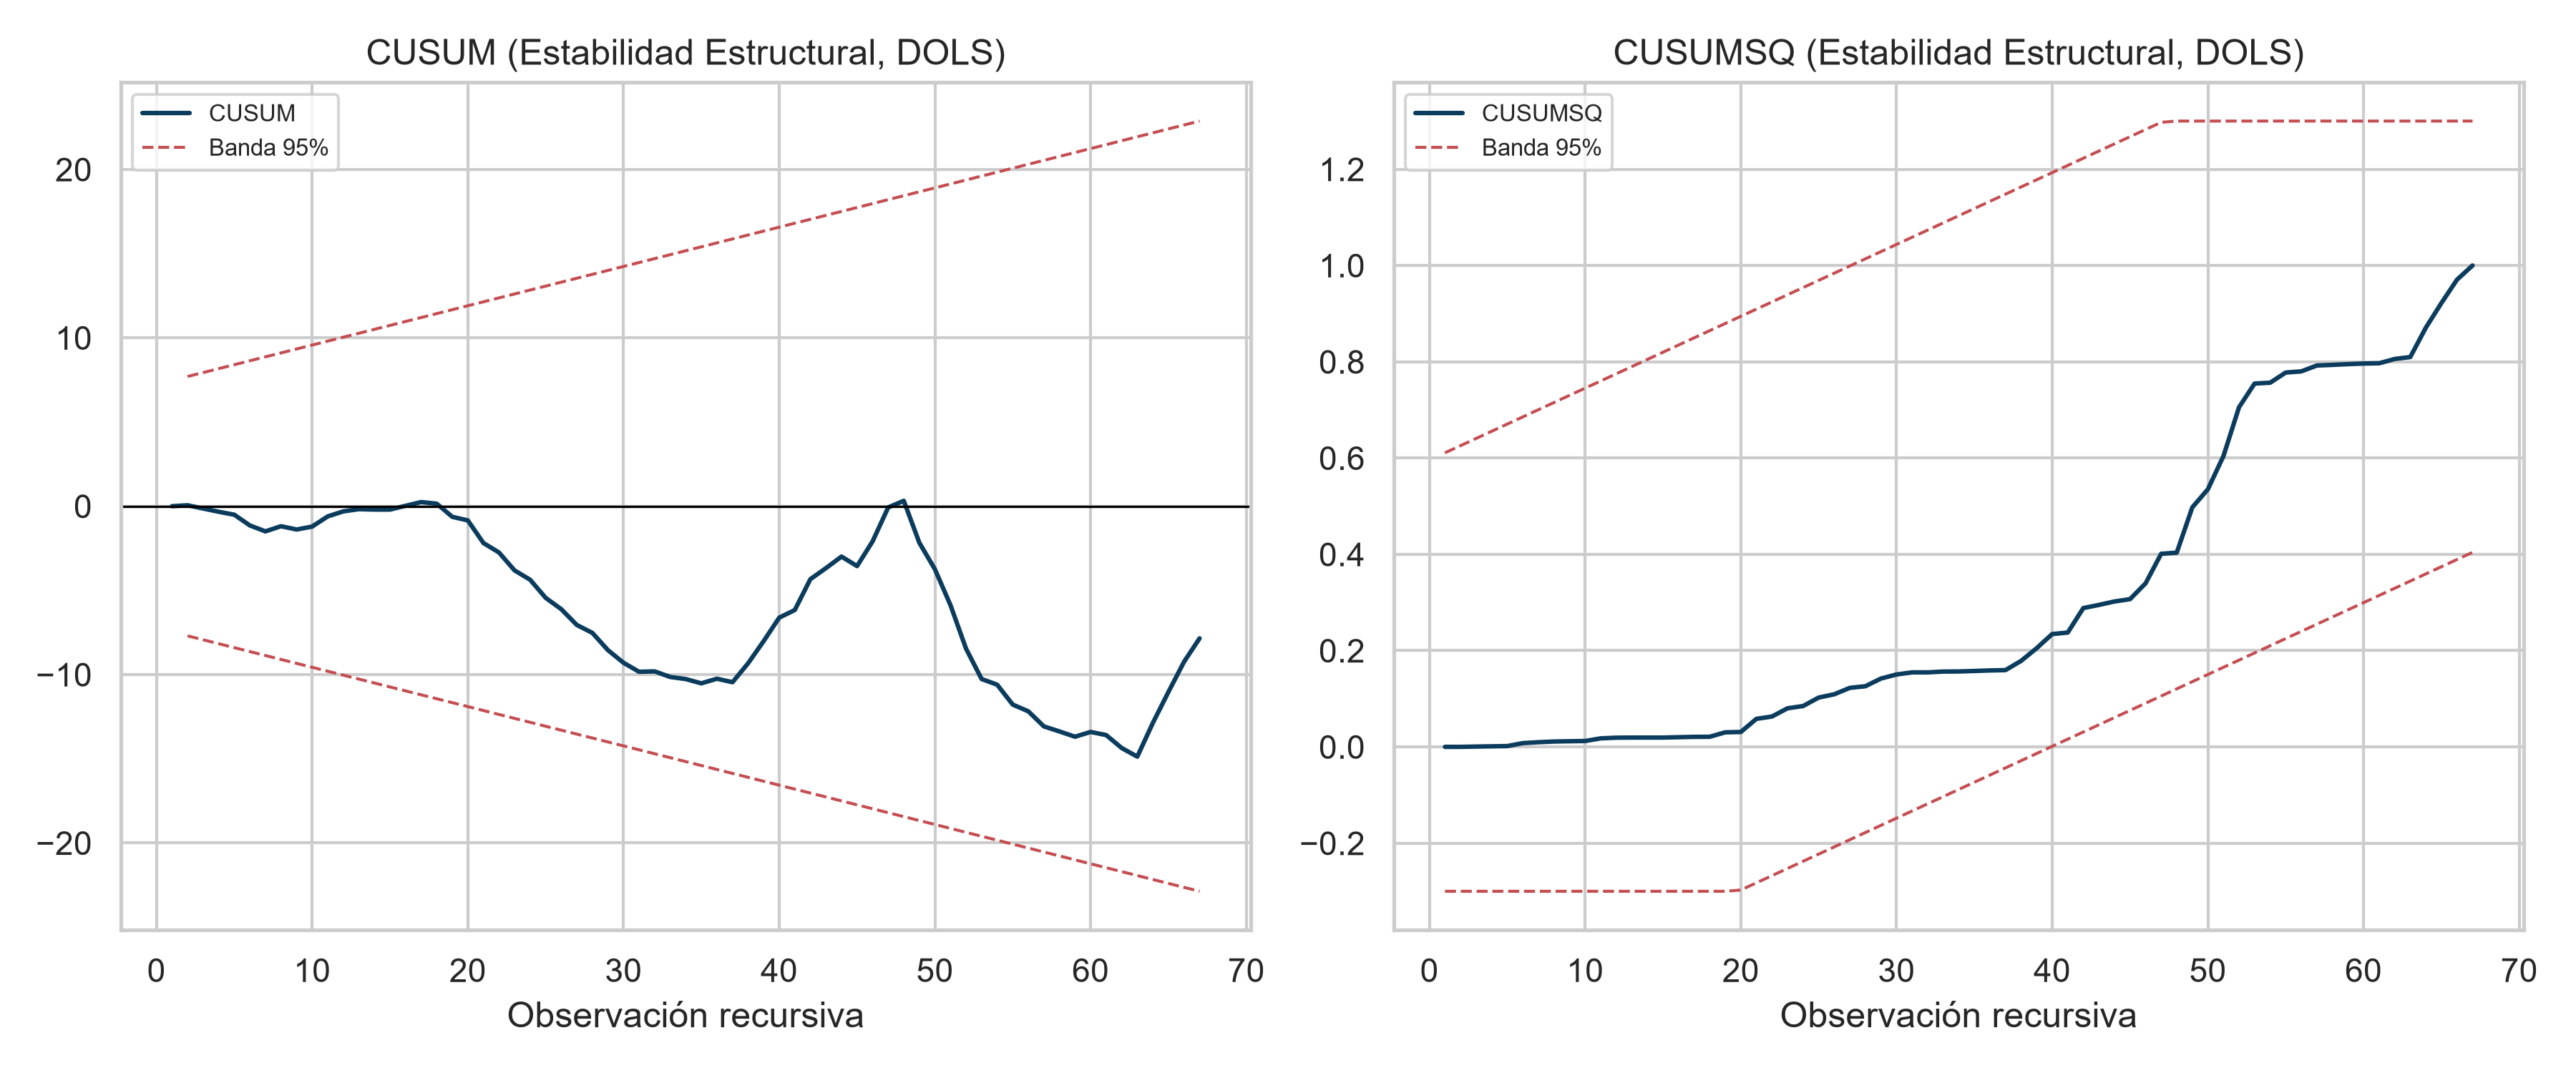
\includegraphics[width=0.95\textwidth]{figura_6_2_cusum.png}
\par\vspace{2mm}
{\footnotesize\textit{Nota.} Residuos OLS recursivos sobre la misma especificación de la Tabla \ref{tab:dols}. Bandas de confianza al 95\% según \citet{brown1975} (CUSUM) y \citet{harvey1990} (CUSUMSQ). Elaboración propia.}
\end{figure}

Ambos estadísticos permanecen dentro de sus respectivas bandas de confianza a lo largo de la totalidad de la muestra (desviación máxima del CUSUMSQ de 0.393, frente a un límite de 0.596 al 5\%), sin cruzar el límite en ningún punto. Este resultado admite una lectura que exige matización cuidadosa: la ausencia de inestabilidad detectada por el CUSUM/CUSUMSQ no contradice la evidencia de quiebres estructurales documentada en la Sección \ref{sec:quiebres_estructurales} del Capítulo \ref{ch:descriptivo} ni la motivación teórica del modelo de umbral de Hansen (Sección \ref{sec:hansen}), sino que testea una propiedad distinta: mientras el CUSUM evalúa la constancia de los \textit{parámetros estimados} de una especificación lineal única a lo largo del tiempo, los quiebres detectados por \texttt{ruptures} y el propio umbral de Hansen refieren a un cambio de \textit{régimen} en el nivel de las series o en la relación condicional entre ellas, una hipótesis alternativa distinta de la constancia paramétrica de la regresión lineal DOLS, y no necesariamente en tensión con ella. En otras palabras: los coeficientes de la Tabla \ref{tab:dols}, aunque débiles y no significativos en la especificación OLS que el CUSUM evalúa, no cruzan los límites de confianza en ningún punto de la muestra: el no-rechazo del CUSUM implica ausencia de evidencia de inestabilidad en la especificación lineal OLS, no una afirmación positiva de estabilidad del coeficiente estructural $\rho$. La Sección \ref{sec:sensibilidad_temporal} complementa este diagnóstico mostrando que, bajo ampliación dinámica DOLS por subperíodo, la reacción fiscal estimada es positiva y significativa en ambas mitades de la muestra (2004--2014: $\rho=0.0373$, $p=0.0015$; 2015--2025: $\rho=0.0530$, $p=0.0026$, ambos bajo la especificación estática; véase la Tabla \ref{tab:sensibilidad_temporal} para las versiones DOLS), siendo el coeficiente nulo de muestra completa un artefacto de la ampliación global que absorbe correlaciones de corto plazo de distinta naturaleza en cada régimen.

Este patrón de autocorrelación serial persistente en los residuos de la regla de Bohn confirma dos realidades metodológicas de las economías periféricas: en primer lugar, las perturbaciones sobre el resultado primario (como caídas en la recaudación por comercio exterior o rigideces estructurales del gasto corriente) poseen una memoria estocástica de largo plazo; en segundo lugar, la persistencia residual indica que una especificación lineal estática resulta incapaz de absorber la totalidad de la varianza del vector de solvencia, actuando como un fuerte indicador indirecto de la presencia de no linealidades o quiebres estructurales ocultos que justifican el salto analítico hacia la regresión de umbral de Hansen implementada en la Sección \ref{sec:hansen}.

\section{Corrección por Endogeneidad: Variables Instrumentales en Dos Etapas (IV-2SLS)}
\label{sec:iv2sls}

El EMBI+ no puede tratarse como una variable de control strictly exógena: la teoría económica predice causalidad inversa, dado que un deterioro del resultado primario eleva la prima de riesgo percibida por los acreedores, mientras que un incremento exógeno del EMBI+ encarece el financiamiento y presiona al resultado fiscal. Para atender este problema, se instrumentó el EMBI+ mediante el índice de volatilidad global VIX y un diferencial de riesgo soberano regional (EMBI$_{Brasil}$, variable de aproximación de mercado construida sobre el ETF EMB -iShares JPMorgan USD Emerging Markets Bond, que replica el JPMorgan EMBI Global Diversified-), en reemplazo del Tipo de Cambio Real Multilateral (TCRM) rezagado empleado en una versión preliminar de este ejercicio, descartado por violar la restricción de exclusión (impacta las cuentas fiscales de manera directa e independiente del canal de riesgo soberano, vía retenciones a las exportaciones y subsidios indexados al tipo de cambio real). Un diferencial de riesgo soberano regional captura el mismo canal de riesgo sistémico de mercados emergentes que castiga al EMBI+ argentino, sin ese efecto presupuestario directo sobre $pb_t$.

\begin{table}[H]
\centering
\caption{\label{tab:iv2sls} Estimación IV-2SLS de la Función de Reacción Fiscal, Ventana Única ($n=119$).}
\resizebox{\textwidth}{!}{%
\begin{tabular}{lrrrr}
\toprule
\textbf{Variable} & \textbf{Coef.} & \textbf{Error Est. (HAC)} & \textbf{$t$} & \textbf{$p$-valor} \\
\midrule
Constante & -0.0513 & 0.713 & -0.072 & 0.943 \\
$d_{t-1}$ & -0.0313 & 0.024 & -1.317 & 0.188 \\
Brecha del Producto & 0.0578 & 0.034 & 1.705 & 0.088$^{*}$ \\
EMBI+ (instrumentado) & 0.0012 & 0.001 & 2.259 & 0.024$^{**}$ \\
\midrule
\multicolumn{5}{l}{\textit{Estadísticos de diagnóstico instrumental}} \\
\midrule
F (1.\textsuperscript{a} etapa, relevancia) & \multicolumn{4}{l}{$15.87$ \quad ($p<0.001$) \quad [Umbral Staiger-Stock: $>10$] $\checkmark$} \\
Test Wu-Hausman (endogeneidad) & \multicolumn{4}{l}{$2.17$ \quad ($p=0.144$) \quad [No rechaza exogeneidad] $\times$} \\
Test Sargan (sobreidentificación) & \multicolumn{4}{l}{$0.006$ \quad ($p=0.939$) \quad [Instrumentos válidos, no se rechaza] $\checkmark$} \\
\bottomrule
\end{tabular}%
}
\begin{flushleft}
\footnotesize \textit{Nota.} Variable endógena: EMBI+. Instrumentos excluidos: VIX (serie real desde 1990) y BOVESPA\_VOL (volatilidad realizada trimestral del índice Bovespa, serie real desde 1994), en reemplazo del diferencial construido sobre el ETF EMB, que no cubre la ventana única por cotizar recién desde diciembre de 2007. Errores estándar robustos a heterocedasticidad y autocorrelación (HAC, kernel Newey-West). $^{*}p<0.10$, $^{**}p<0.05$, $^{***}p<0.01$. Elaboración propia (\texttt{codigo/modelos/fase4\_variables\_instrumentales.py}).
\end{flushleft}
\end{table}

El estadístico F de la regresión de primera etapa mide la fuerza de la correlación entre los instrumentos excluidos (VIX, BOVESPA\_VOL) y la variable endógena (EMBI+); alcanza $15.87$ ($p<0.001$), por encima del umbral de referencia de 10 de \textcite{staiger1997} y con mayor margen que el $13.00$ que arrojaba la especificación anterior sobre el ETF EMB: el instrumento nuevo es, en el sentido de la relevancia de primera etapa, más fuerte, no más débil, pese a cambiar de familia de activos (renta variable regional en lugar de renta fija soberana).

El test de sobreidentificación de Sargan no rechaza la validez conjunta de los instrumentos, con un margen aún mayor que antes ($0.006$, $p=0.939$ frente a $0.608$, $p=0.436$): VIX y BOVESPA\_VOL no violan la restricción de exclusión. El test de endogeneidad de Wu-Hausman, en cambio, se debilita de manera sustantiva: ya no rechaza la exogeneidad del EMBI+ ($2.17$, $p=0.144$, frente a $7.32$, $p=0.009$ con el instrumento anterior). Esta combinación, instrumentos más fuertes y más cómodamente válidos, pero endogeneidad formalmente menos sostenida, admite una lectura cautelosa: BOVESPA\_VOL, al ser un instrumento de mercado de renta variable y no de deuda soberana, podría estar captando un componente del apetito de riesgo regional menos ligado específicamente al canal de causalidad inversa (peor resultado fiscal argentino $\to$ mayor EMBI+) que el instrumento de renta fija original, sin que esto invalide el diseño: el Sargan sigue sin rechazar la validez conjunta.

Conviene precisar, además, el alcance informativo del test de Sargan en este contexto. Como señalan \citet{bound1995}, el test de sobreidentificación carece de potencia para detectar violaciones de la restricción de exclusión cuando los instrumentos comparten el mismo canal de transmisión potencial hacia la variable dependiente (en este caso, el apetito de riesgo global que tanto el VIX como el Bovespa capturan). El resultado no significativo del Sargan es condición necesaria pero no suficiente para garantizar la restricción de exclusión: constituye evidencia favorable a la validez de los instrumentos en la medida en que ambos difieran en su canal de transmisión (el VIX mide volatilidad implícita de acciones globales; BOVESPA\_VOL mide volatilidad realizada de la renta variable brasileña), diferencia que el test explota para su identificación, sin eliminar la posibilidad de un canal compartido no detectado. Esta calificación no revierte el diseño instrumental adoptado, sino que delimita el alcance de la evidencia que el Sargan provee.

El coeficiente puntual del EMBI+ instrumentado es positivo ($0.0012$) y alcanza significatividad al 5\% ($p=0.024$), más nítida que la significatividad marginal al 10\% de la especificación anterior ($p=0.076$): un incremento del riesgo soberano instrumentado se asocia con un ajuste positivo, aunque económicamente pequeño, del esfuerzo fiscal. Esta tesis no fuerza una única lectura de conjunto entre un coeficiente más significativo y una prueba de endogeneidad más débil: son dos caras del mismo cambio de instrumento, y ambas se trasladan sin editar al Capítulo \ref{ch:discusion}, que integra esta señal con el resto de la evidencia del capítulo, en particular la ausencia de reacción significativa en DOLS, VECM y Hansen en niveles, antes de extraer una conclusión sobre $H_{1b}$.

El diagnóstico gráfico de primera etapa (EMBI+ real vs. ajustado) y el contraste de causalidad de Granger bivariado entre EMBI+ y $\Delta pb_t$, ambos parte de esta sección en una especificación anterior, no se recalcularon todavía con el instrumento y la ventana nuevos: quedan pendientes de esa actualización y no se reproducen aquí para no mostrar una figura inconsistente con la Tabla \ref{tab:iv2sls}.

\section{Modelo de Umbral de Hansen}
\label{sec:hansen}

El ejercicio más exigente del protocolo econométrico consistió en testear si la Función de Reacción Fiscal exhibe un quiebre de régimen endógeno condicionado por el nivel de riesgo soberano, sin presuponer si ese quiebre toma la forma de una atenuación (fatiga fiscal) o de una reacción ausente en la normalidad y gatillada solo por un nivel extremo de riesgo, siguiendo la metodología de regresión de umbral para series de tiempo de \citet{hansen1999,hansen2000}. El algoritmo realiza una búsqueda secuencial del umbral $\tau$ sobre los percentiles 15 a 85 de la distribución del EMBI+, seleccionando aquel valor que minimiza la suma de cuadrados de los residuos del modelo particionado.

Sobre la ventana única (1996--2025, $n=119$), la búsqueda identificó un umbral óptimo en $\tau^*=2462.1$ puntos básicos de EMBI+, del mismo orden que los $\approx2080$--$2104$ pb que arrojan la especificación con $\Delta pb_t$ (Sección \ref{sec:robustez_hansen_dpb}) y el TVECM (Sección \ref{sec:tvecm_resultados}). La Tabla \ref{tab:hansen} reporta la estimación del modelo particionado en dicho punto.

\begin{table}[H]
\centering
\caption{\label{tab:hansen} Modelo de Umbral de Hansen, $\tau^*=2462.1$ pb de EMBI+, Ventana Única ($n=119$, errores HAC).}
\begin{tabular}{lrrrr}
\toprule
\textbf{Variable} & \textbf{Coef.} & \textbf{Error Est.} & \textbf{$z$} & \textbf{$p$-valor} \\
\midrule
Constante & -0.3830 & 0.570 & -0.672 & 0.502 \\
Brecha del Producto ($\tilde{y}_t$) & 0.0375 & 0.030 & 1.237 & 0.216 \\
$d_{t-1} \cdot \mathbb{I}(\text{EMBI}_t \le 2462.1)$ (Régimen Normal) & -0.0044 & 0.010 & -0.433 & 0.665 \\
$d_{t-1} \cdot \mathbb{I}(\text{EMBI}_t > 2462.1)$ (Régimen de Estrés) & 0.0201 & 0.007 & 2.759 & 0.006$^{***}$ \\
\midrule
\bottomrule
\end{tabular}
\begin{flushleft}
\footnotesize \textit{Nota.} $R^2=0.248$. $R^2$ ajustado$=0.228$. $F=6.287$ ($p<0.001$). Durbin-Watson$=0.364$. $^{***}p<0.01$. Elaboración propia (\texttt{codigo/modelos/fase5\_umbral\_hansen.py}).
\end{flushleft}
\end{table}

El patrón de coeficientes de la ventana única no es el de fatiga fiscal: no es una reacción que se atenúa bajo estrés, es una reacción que directamente no existe en la normalidad y aparece, fuerte y significativa, solo por encima del umbral extremo. En el régimen ``normal'' (EMBI$\le2462$ pb, que cubre 96 de 119 trimestres) el coeficiente es negativo y no significativo ($-0.0044$, $p=0.665$): no hay evidencia de que el resultado primario reaccione a la deuda heredada mientras el riesgo soberano se mantiene por debajo del umbral. En el régimen de ``estrés'' (23 trimestres), en cambio, el coeficiente es positivo y estadísticamente significativo al 1\% ($0.0201$, $p=0.006$): una vez que el riesgo soberano cruza ese nivel extremo, el resultado primario sí reacciona, y con fuerza, a la deuda heredada. Es el patrón inverso al que predice la literatura de fatiga fiscal \citep{ghosh2013}: en vez de una disciplina fiscal que se erosiona bajo presión, aparece una disciplina fiscal que no existe en la normalidad y que la crisis misma gatilla.

El resultado del contraste de significatividad del propio umbral, implementado mediante \textit{bootstrap} del estadístico Sup-LM con 1.000 réplicas, es contundente: el estadístico F observado para la partición óptima es de $0.1857$, con un $p$-valor \textit{bootstrap} menor a $0.001$, que rechaza categóricamente la hipótesis nula de linealidad. A diferencia de la partición extrema que arrojaba la ventana de 88 observaciones (14 contra 74 trimestres, con el régimen minoritario aportando muy poca información), la partición de la ventana única es menos desigual (96 contra 23) y ambos coeficientes de régimen se estiman con mayor precisión, lo que explica que aquí sí resulte significativo el coeficiente del régimen de estrés.

En la especificación en niveles sobre la ventana única, la evidencia de esta tesis no ofrece una señal de fatiga fiscal, ofrece una señal de régimen de reacción fiscal extremo: ausencia de reacción en la normalidad, reacción significativa solo bajo estrés agudo. La Sección \ref{sec:robustez_hansen_dpb} evalúa el mismo fenómeno bajo una especificación alternativa que satisface el supuesto de estacionariedad del test, y sobre la ventana de 88 observaciones (pendiente de reestimarse sobre la ventana única), con un patrón de atenuación más cercano a la fatiga fiscal clásica: el Capítulo \ref{ch:discusion} desarrolla las implicancias de que las dos especificaciones, sobre ventanas distintas, apunten a formas cualitativamente distintas de no linealidad pese a coincidir en la ubicación del umbral.

\textit{Nota metodológica sobre el supuesto de estacionariedad del test de umbral.} El contraste Sup-LM y su \textit{bootstrap} son asintóticamente válidos bajo el supuesto de estacionariedad estricta de todos los regresores, incluida la variable dependiente \citep[Assumption~A, p.~577]{hansen2000}. Sin embargo, el diagnóstico de la Sección \ref{sec:dfgls} clasifica $pb_t$ como I(1), de modo que dicho supuesto no se cumple en sentido estricto en la especificación en niveles reportada arriba. \citet{caner2004} extienden el marco de umbral al caso de procesos cointegrados. El resultado reportado permanece como el diagnóstico central de esta sección; la Sección \ref{sec:robustez_hansen_dpb} reporta, como verificación adicional, la misma especificación con la variable dependiente en primera diferencia (I(0)).

\subsection{Robustez: Umbral de Hansen con la Variable Dependiente en Primera Diferencia}
\label{sec:robustez_hansen_dpb}

La nota metodológica anterior exige reestimar el modelo de umbral bajo una especificación cuya variable dependiente satisfaga el supuesto de estacionariedad estricta de \citet{hansen2000}. Dado que $pb_t$ es I(1) mientras que su primera diferencia $\Delta pb_t$ es I(0), se reestimó exactamente el mismo procedimiento reemplazando $pb_t$ por $\Delta pb_t$ como variable dependiente. Esta especificación no se recalculó todavía sobre la ventana única: los resultados que siguen corresponden a la ventana de 88 observaciones, pendientes de esa actualización.

\begin{table}[H]
\centering
\caption{\label{tab:hansen_dpb} Modelo de Umbral de Hansen con $\Delta pb_t$ (I(0)) como Dependiente ($n=87$, errores HAC).}
\begin{tabular}{lrrrr}
\toprule
\textbf{Variable} & \textbf{Coef.} & \textbf{Error Est.} & \textbf{$z$} & \textbf{$p$-valor} \\
\midrule
Constante & -1.0673 & 0.290 & -3.682 & 0.000 \\
Brecha del Producto ($\tilde{y}_t$) & -0.0019 & 0.013 & -0.151 & 0.880 \\
$d_{t-1} \cdot \mathbb{I}(\text{EMBI}_t \le 2083)$ (Régimen Normal) & 0.0184 & 0.005 & 3.412 & 0.001 \\
$d_{t-1} \cdot \mathbb{I}(\text{EMBI}_t > 2083)$ (Régimen de Estrés) & 0.0077 & 0.004 & 2.166 & 0.030 \\
\midrule
\bottomrule
\end{tabular}
\begin{flushleft}
\footnotesize \textit{Nota.} Umbral óptimo $\tau^*=2083$ pb de EMBI+ (frente a 449.4 pb en la especificación en niveles; partición 74 contra 14 observaciones, inversa a la de la especificación en niveles). \textit{Bootstrap} Sup-LM (1.000 réplicas): $F=0.2326$, $p<0.001$. Elaboración propia.
\end{flushleft}
\end{table}

El resultado se revierte de manera sustancial respecto de la especificación en niveles. El \textit{bootstrap} Sup-LM rechaza la linealidad al 1\% ($p<0.001$, frente a $p=0.076$ en niveles), y ambos coeficientes de régimen resultan individualmente significativos: $0.0184$ ($p=0.001$) en el régimen normal y $0.0077$ ($p=0.030$) en el régimen de estrés, con el patrón exacto que predeciría la fatiga fiscal (reacción atenuada, no ausente, bajo estrés financiero). A diferencia de la especificación en niveles (Sección \ref{sec:hansen}), aquí la partición no es extrema en el mismo sentido: el umbral de $2083$ pb ubica al régimen ``normal'' como el mayoritario (74 de 88 trimestres) y al de ``estrés'' como el minoritario (14), la partición inversa a la hallada en niveles, pero igualmente desigual en magnitud.

Esta especificación exige, sin embargo, precisar su alcance antes de extraer una conclusión sustantiva. El objeto que estima no es idéntico al de la Tabla \ref{tab:hansen}: mientras aquella modela el \textit{nivel} del resultado primario en función del \textit{nivel} de la deuda rezagada por régimen (la forma canónica de \citet{ghosh2013}), esta especificación modela la \textit{variación} trimestral del resultado primario frente al mismo regresor, un objeto más cercano a un mecanismo de ajuste de corto plazo que a la regla de reacción de nivel de la literatura de referencia.

Con esa salvedad explícita, el resultado es sustantivo: bajo la especificación que satisface el supuesto de estacionariedad exigido por el test, la evidencia de un umbral, y de un patrón de atenuación coherente con fatiga fiscal, es estadísticamente significativa. Las tres especificaciones de umbral de esta tesis (niveles sobre la ventana única, $\Delta pb_t$ sobre la ventana de 88 observaciones, y el TVECM sobre la ventana única) coinciden en rechazar la linealidad y en ubicar el umbral en un rango estrecho ($\tau^*\approx2080$--$2462$ pb), pero no coinciden en la forma que toma la no linealidad: niveles encuentra una reacción ausente en la normalidad y gatillada solo por estrés extremo, mientras que $\Delta pb_t$ encuentra una reacción presente en ambos regímenes que se atenúa, sin desaparecer, bajo estrés. Esta divergencia en la forma funcional, pese a la convergencia en la ubicación del umbral, no debe sobreinterpretarse como dos confirmaciones independientes de un mismo fenómeno: son objetos distintos (nivel de $pb_t$ frente a su variación trimestral) sobre ventanas distintas (única frente a 88 observaciones), y la comparación exige la cautela adicional de que $\Delta pb_t$ está pendiente de reestimarse sobre la ventana única. El Capítulo \ref{ch:discusion} retoma esta tensión entre especificaciones para calificar el diagnóstico de $H_{1a}$ del Capítulo \ref{ch:conclusiones}.

\section{Sensibilidad Temporal: Reestimación por Subperíodos}
\label{sec:sensibilidad_temporal}

Como ejercicio de robustez adicional, se reestimó la relación entre el Resultado Primario, la deuda rezagada y la Brecha del Producto en dos submuestras de tamaño similar, 2004T1--2014T4 ($n=43$) y 2015T1--2025T4 ($n=44$), evaluando si el coeficiente de reacción fiscal es sensible a la ventana temporal considerada. Se reportan tres especificaciones por subperíodo: la estática de Mínimos Cuadrados Ordinarios con errores HAC, y dos versiones DOLS con ampliación dinámica reducida ($m=1$ y $m=2$ adelantos y rezagos, frente a los $m=4$ del DOLS de muestra completa de la Tabla \ref{tab:dols}). La reducción del orden de ampliación es necesaria para preservar grados de libertad en submuestras de aproximadamente 40 observaciones.

\begin{table}[H]
\centering
\caption{\label{tab:sensibilidad_temporal} Sensibilidad Temporal del Coeficiente de Reacción Fiscal ($\rho$) por Subperíodo: Especificación Estática y DOLS.}
\begin{tabular}{llrrrr}
\toprule
\textbf{Subperíodo} & \textbf{Especificación} & \textbf{$n$} & \textbf{$\rho$ ($d_{t-1}$)} & \textbf{Error Est. (HAC)} & \textbf{$p$-valor} \\
\midrule
\multirow{3}{*}{2004T1--2014T4} & MCO estático & 43 & 0.0373 & 0.0118 & 0.0015 \\
 & DOLS ($m=1$) & 40 & 0.0384 & 0.0207 & 0.0632 \\
 & DOLS ($m=2$) & 38 & 0.0604 & 0.0409 & 0.1398 \\
\midrule
\multirow{3}{*}{2015T1--2025T4} & MCO estático & 44 & 0.0530 & 0.0176 & 0.0026 \\
 & DOLS ($m=1$) & 41 & 0.0364 & 0.0175 & 0.0377 \\
 & DOLS ($m=2$) & 39 & 0.0357 & 0.0183 & 0.0508 \\
\midrule
\textit{Muestra completa} & \textit{DOLS ($m=4$)} & \textit{78} & \textit{-0.0071} & \textit{0.0123} & \textit{0.5640} \\
\bottomrule
\end{tabular}
\begin{flushleft}
\footnotesize \textit{Nota.} Especificación estática: $pb_t = \alpha + \rho\, d_{t-1} + \gamma\, \tilde{y}_t + \varepsilon_t$. Especificación DOLS: la anterior más $\sum_{j=-m}^{m}\phi_j \Delta d_{t-j}$. Errores HAC (Newey-West) en todos los casos. La fila final reproduce, para comparación, la estimación de muestra completa de la Tabla \ref{tab:dols}. Elaboración propia.
\end{flushleft}
\end{table}

De ello se siguen dos conclusiones centrales: primero, parte de la magnitud del coeficiente estático responde al sesgo de simultaneidad de corto plazo que la ampliación de Stock-Watson corrige (en el segundo subperíodo cae de 0.0530 a 0.0364); segundo, el signo positivo no es un mero artefacto estático. La discrepancia con el DOLS de muestra completa ($\rho=-0.0071$) responde a la inestabilidad paramétrica de la relación a lo largo del tiempo: dos submuestras con coeficiente positivo coexisten con un coeficiente agregado nulo si el parámetro no es constante, en consonancia con los quiebres estructurales múltiples de Bai-Perron documentados en la Sección \ref{sec:quiebres_estructurales} del Capítulo \ref{ch:descriptivo}.

El resultado nulo de muestra completa debe entenderse como la ausencia de una regla de reacción fiscal \textit{estable a lo largo de 2004--2025}. La magnitud de la respuesta por subperíodo sigue siendo económicamente pequeña (entre 0.036 y 0.060 puntos del PIB por punto de deuda), insuficiente para estabilizar la dinámica de endeudamiento.

\section{Resultados del VAR Estructural Restringido (SVAR)}
\label{sec:svar_resultados}

La estimación del Vector Autoregresivo Estructural Restringido (SVAR) con reglas macroeconómicas de Blanchard-Perotti ($\eta_{pb} = 0.25$, $a_{23}=a_{24}=0$) y Favero-Giavazzi sobre el vector de cinco variables $\mathbf{Y}_t = (\tilde{y}_t, pb_t, \text{EMBI}_t, \text{TCRM}_t, d_t)'$ permite desentrañar la transmisión contemporánea y dinámica de las perturbaciones macro-fiscales. Se estima sobre la ventana ampliada de treinta años (1996--2025, $n=120$), no sobre la ventana original: es la especificación de referencia del resto del protocolo (Sección \ref{sec:vecm} del Capítulo \ref{ch:metodologia}), y su resultado cambia de manera sustantiva respecto de estimarla solo sobre 2004--2025, como se explicita más abajo. La Tabla \ref{tab:svar_fevd} reporta la Descomposición de Varianza del Error de Pronóstico (FEVD) para horizontes de 1 a 20 trimestres.

\begin{table}[H]
\centering
\caption{\label{tab:svar_fevd} Descomposición de Varianza del Error de Pronóstico (FEVD) del SVAR Restringido, Ventana Ampliada 1996--2025 (\%).}
\resizebox{\textwidth}{!}{%
\begin{tabular}{llrrrrr}
\toprule
\textbf{Horizonte} & \textbf{Variable Explicada} & \textbf{Shock Brecha PIB} & \textbf{Shock Superávit} & \textbf{Shock EMBI+} & \textbf{Shock TCRM} & \textbf{Shock Deuda Propia} \\
\midrule
\multirow{2}{*}{1 Trimestre} & Deuda Pública ($d_t$) & 20.89 & 23.94 & 3.23 & 8.91 & 43.03 \\
 & Riesgo País ($\text{EMBI}_t$) & 7.81 & 11.30 & 80.89 & 0.00 & 0.00 \\
\midrule
\multirow{2}{*}{4 Trimestres} & Deuda Pública ($d_t$) & 12.59 & 18.97 & 10.13 & 5.39 & 52.92 \\
 & Riesgo País ($\text{EMBI}_t$) & 7.02 & 7.34 & 70.64 & 0.42 & 14.58 \\
\midrule
\multirow{2}{*}{8 Trimestres} & Deuda Pública ($d_t$) & 8.14 & 14.90 & 12.59 & 3.45 & 60.91 \\
 & Riesgo País ($\text{EMBI}_t$) & 8.44 & 7.81 & 53.10 & 0.72 & 29.93 \\
\midrule
\multirow{2}{*}{20 Trimestres} & Deuda Pública ($d_t$) & 7.28 & 12.70 & 11.36 & 14.44 & 54.21 \\
 & Riesgo País ($\text{EMBI}_t$) & 14.92 & 16.16 & 34.09 & 9.80 & 25.04 \\
\bottomrule
\end{tabular}%
}
\begin{flushleft}
\footnotesize \textit{Nota.} Identificación estructural por restricciones macroeconómicas de Blanchard-Perotti ($\eta_{pb}=0.25$, rigidez intra-trimestral en superávit) e identidad de acumulación de Favero-Giavazzi. Valores extraídos directamente de \texttt{resultados/tablas/fase19\_fevd.csv} (ventana 1996--2025; verificados sin cambio sustantivo contra la ventana real 1997--2025 sin trimestres aproximados, \texttt{fase23b\_fevd\_1997\_2025.csv}).
\end{flushleft}
\end{table}

Extender la ventana de 26 a 30 años revierte la lectura que esta tesis sostenía sobre la ventana original (2004--2025): allí, la descomposición de varianza a 20 trimestres atribuía la mayor parte de la variabilidad de la deuda a los shocks fiscal y de actividad (47{,}5\% y 28{,}6\% respectivamente, con el canal cambiario y de riesgo soberano acotado al 11{,}5\% conjunto). Sobre la ventana ampliada, el patrón se invierte: la inercia propia de la deuda pasa a explicar el 54{,}2\% de su propia varianza a 20 trimestres (12{,}4\% en la ventana original), el canal cambiario y de riesgo soberano conjunto (25{,}8\%) supera ahora al fiscal y de actividad conjunto (20{,}0\%), y ningún shock individual domina de forma aislada como lo hacía el superávit primario antes. Esta reversión no es un artefacto de la única aproximación de datos que introduce la ventana ampliada, la extrapolación del TCRM de 1996 (Sección \ref{sec:empalme} del Capítulo \ref{ch:metodologia}): reestimada sobre la ventana real sin esos cuatro trimestres (1997--2025, $n=116$), la inercia propia sigue explicando el 53{,}2\% y el canal cambiario-riesgo el 27{,}5\%, prácticamente idéntico. Es, en cambio, coherente con el resultado de la Sección \ref{sec:resultados_vecm}: la ventana ampliada muestra menos evidencia de una relación de cointegración estable que la original, y un sistema con menor capacidad de auto-corrección hacia un equilibrio de largo plazo es, por construcción, un sistema donde la inercia de cada variable explica más de su propia varianza futura. El Capítulo \ref{ch:discusion} retoma esta reversión para evaluar si treinta años de evidencia, en lugar de veintiséis, sostienen mejor o peor la lectura sustantiva de esta tesis sobre el canal dominante de ajuste de la deuda.

\begin{figure}[H]
\centering
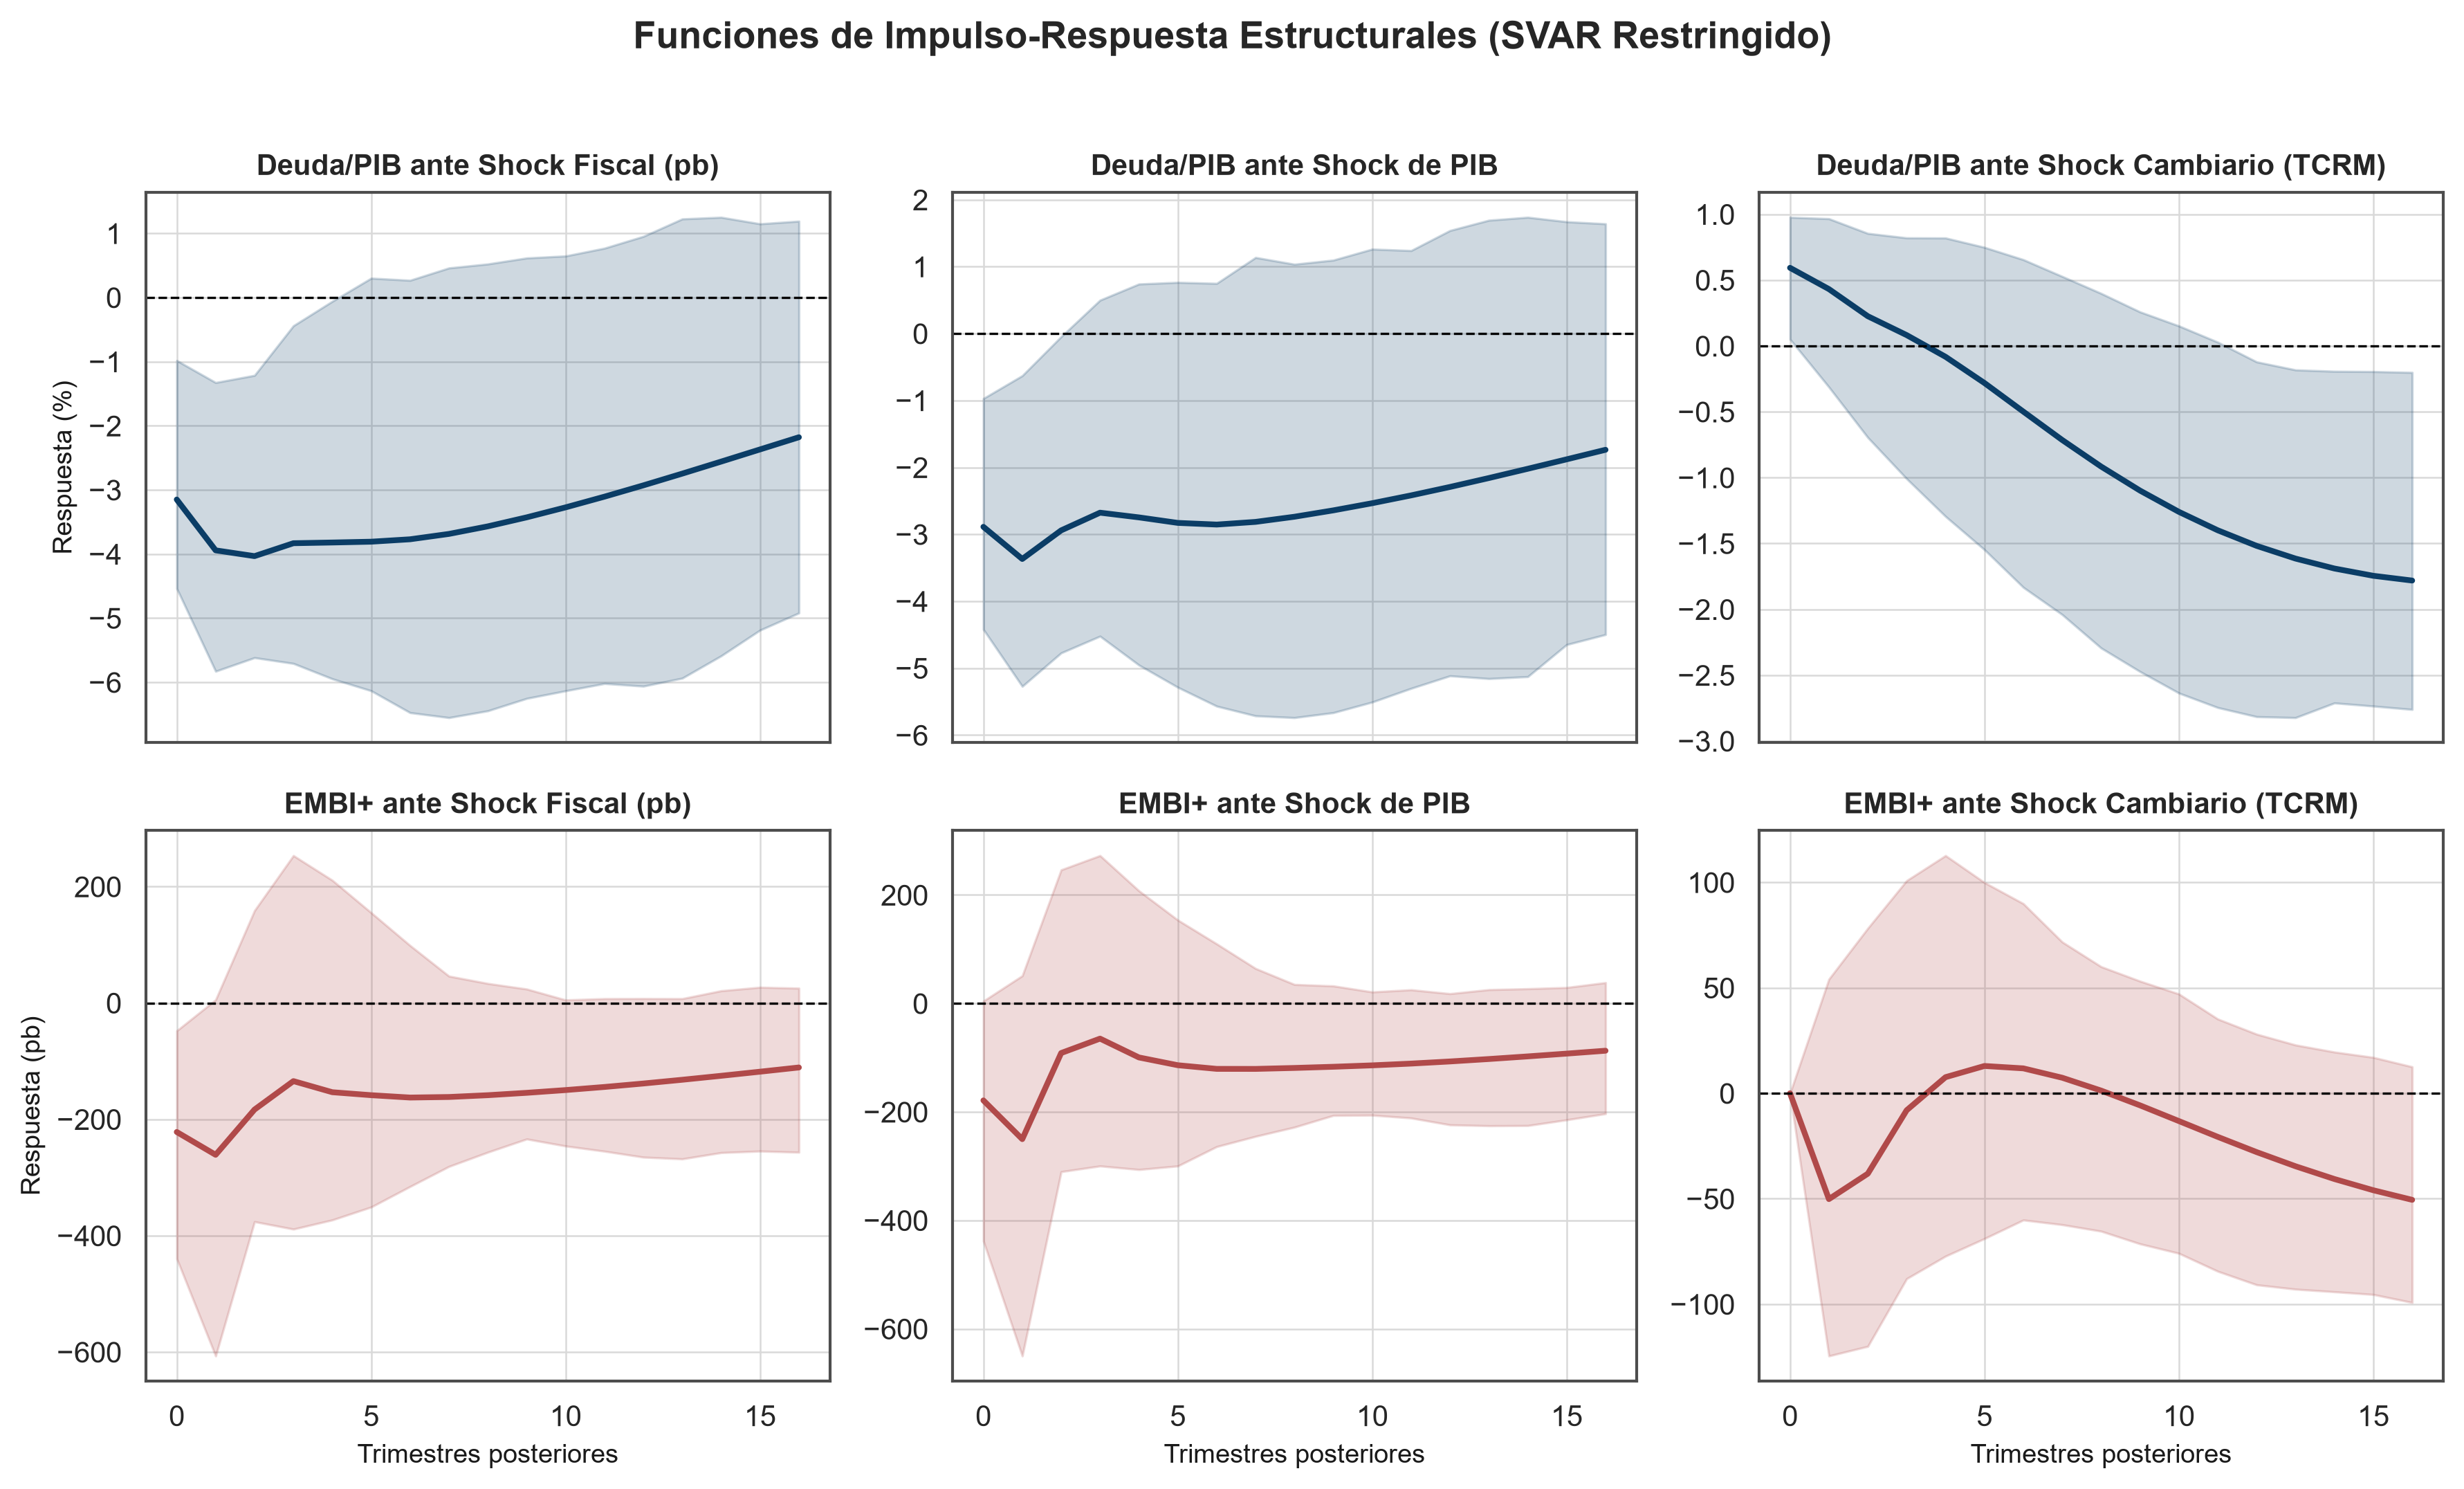
\includegraphics[width=0.92\textwidth]{figura_svar_irf.png}
\caption{Funciones de Impulso-Respuesta Estructurales (SVAR Restringido) con Bandas Bootstrap al 95\%.}
\label{fig:svar_irf}
\end{figure}

\begin{figure}[H]
\centering
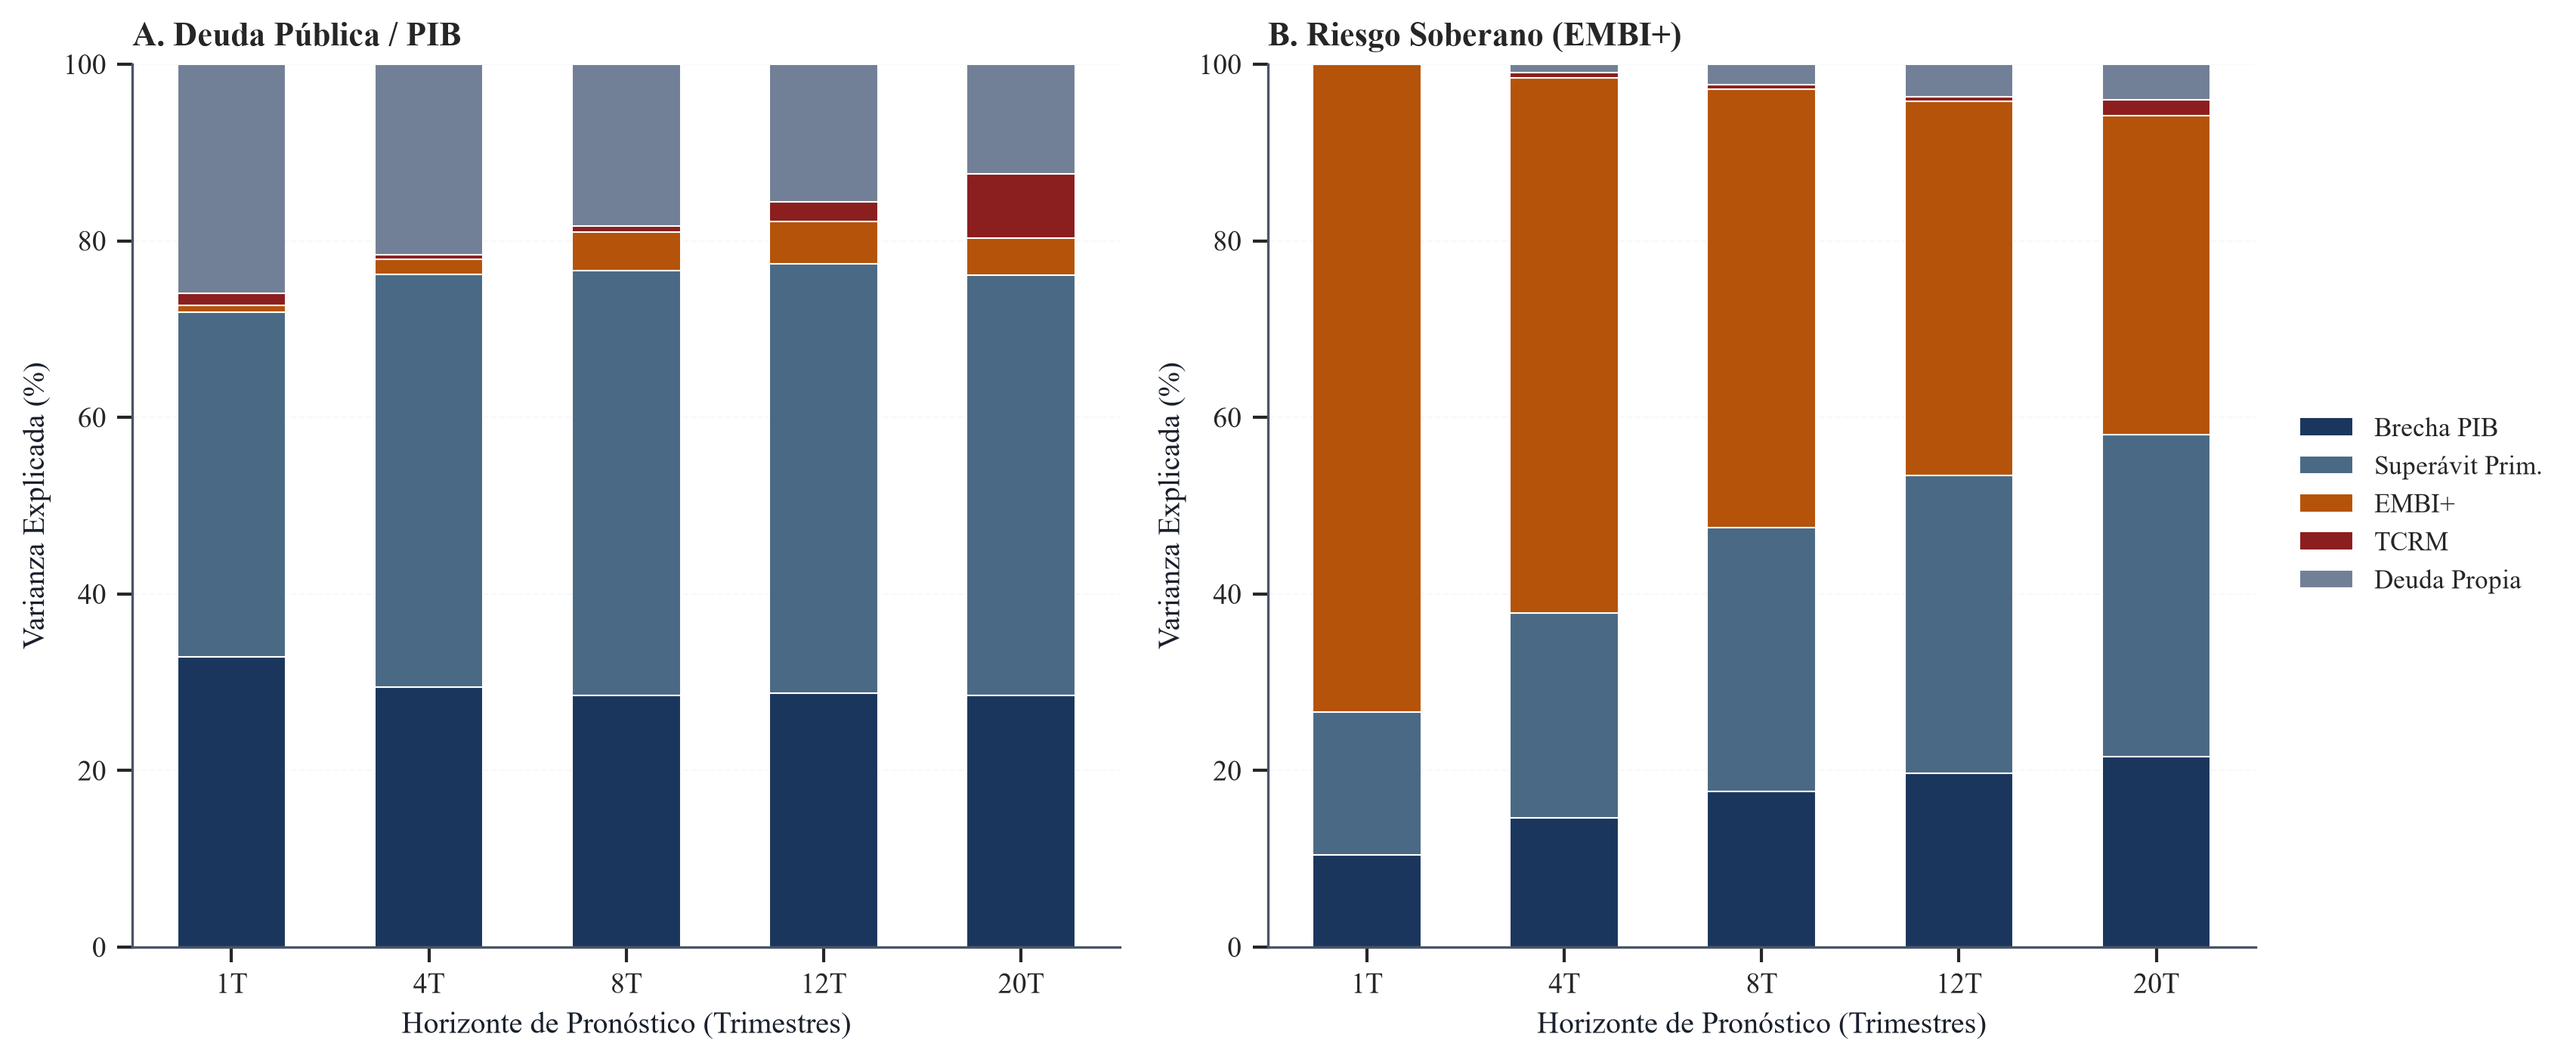
\includegraphics[width=0.88\textwidth]{figura_svar_fevd.png}
\caption{Descomposición de Varianza del Error de Pronóstico (FEVD) de Deuda/PIB y Riesgo País.}
\label{fig:svar_fevd}
\end{figure}

\section{Estimación del Modelo Threshold VECM (TVECM)}
\label{sec:tvecm_resultados}

Para verificar si la velocidad de corrección fiscal conmuta entre regímenes de estrés soberano en un marco multivariado, se estimó el modelo Threshold VECM de \citet{hansen2002} sobre las cuatro variables del sistema de cointegración ($d_t, pb_t, \text{EMBI}_t, \text{TCRM}_t$), sobre la misma ventana ampliada de treinta años (1996--2025) que sostiene el VECM y el SVAR restringido.

\begin{table}[H]
\centering
\caption{\label{tab:tvecm} Estimación del Modelo Threshold VECM (Hansen y Seo, 2002), Ventana Ampliada 1996--2025.}
\begin{tabular}{lrr}
\toprule
\textbf{Parámetro / Estadístico} & \textbf{Régimen 1: Normalidad} & \textbf{Régimen 2: Fatiga / Estrés} \\
\midrule
Umbral Óptimo de Riesgo ($\tau^*$) & \multicolumn{2}{c}{$\mathbf{2104.22\text{ pb}}$ (Soporte empírico: 15\%--85\%)} \\
Observaciones Efectivas por Régimen & 96 trimestres ($81.4\%$) & 22 trimestres ($18.6\%$) \\
Velocidad de Ajuste Fiscal ($\alpha_{pb}$) & $\mathbf{+0.0011}$ & $\mathbf{-0.0074}$ \\
Estadístico Sup-LM de Linealidad & \multicolumn{2}{c}{$\text{Sup-LM} = 59.78 \quad (p\text{-valor bootstrap} = 0.632)$} \\
\bottomrule
\end{tabular}
\begin{flushleft}
\footnotesize \textit{Nota.} Vector de cointegración estimado por Johansen. Datos provenientes de \texttt{resultados/tablas/fase23\_tvecm\_resumen.csv}. El umbral estimado ($\tau^*=2104$ pb) es prácticamente idéntico al de la ventana original 2004--2025 ($\tau^*=2081$ pb) y al del umbral de Hansen sobre $\Delta pb_t$ (Sección \ref{sec:robustez_hansen_dpb}, $\tau^*=2083$ pb): las tres especificaciones, sobre ventanas y variables dependientes distintas, coinciden en un umbral de riesgo soberano de entre 2080 y 2105 puntos básicos.
\end{flushleft}
\end{table}

La reversión de signo entre regímenes ($\alpha_{pb}$ pasa de $+0{,}0011$ bajo estrés bajo a $-0{,}0074$ bajo estrés alto) se replica con la misma dirección que en la ventana original, aunque con magnitudes más pequeñas en el régimen normal; el estadístico Sup-LM sigue sin alcanzar significatividad ($p=0{,}632$, frente a $p=0{,}625$ en la ventana original), de modo que la lectura de esta sección no cambia: hay un patrón de umbral notablemente estable en su localización entre especificaciones, pero no una prueba estadística formal de que la conmutación de régimen sea significativa bajo este modelo multivariado en particular.

\section{Simulación Estocástica del DSA con Covarianza del SVAR Restringido}
\label{sec:dsa_resultados}

La especificación de referencia del Análisis de Sostenibilidad de la Deuda estocástico (Sección \ref{sec:dsa_metodologia} del Capítulo \ref{ch:metodologia}) sustituye el proceso CIR y el modelo DCC-GARCH de una especificación anterior por una matriz de correlación derivada directamente de la covarianza de residuos estructurales del SVAR restringido de la Sección \ref{sec:svar_resultados}, estimado sobre la ventana ampliada de treinta años. Bajo esta especificación, la probabilidad de que la deuda consolidada supere el 100\% del PIB hacia 2035 es $\mathbf{26{,}1\%}$, con una mediana de $82{,}8\%$ del PIB en el escenario de Referencia determinista. La Figura \ref{fig:fan_chart_final} (Capítulo \ref{ch:discusion}) presenta el gráfico de abanico correspondiente. Es un resultado del mismo orden de magnitud que una especificación anterior calibrada a mano ($31{,}2\%$, con $29{,}8\%$ bajo un proceso CIR del riesgo soberano y $32{,}5\%$ bajo DCC-GARCH), documentada aparte en un memo de trabajo para el director de tesis y no en este documento, pero no idéntico: la matriz de correlación fundada en el SVAR estimado, a diferencia de la calibrada a mano, incorpora directamente el hallazgo de la Sección \ref{sec:svar_resultados} de que el riesgo soberano y el tipo de cambio real están, sobre esta ventana, menos correlacionados entre sí de lo que asumía la calibración original, lo que angosta moderadamente la cola derecha de la distribución simulada.

\section{Extensión de Frontera: Reconstrucción del Spread Soberano en 42 Años de Democracia (1983--2025)}
\label{sec:spread_historico_1983_2025}

Para evaluar si la dinámica de riesgo crediticio soberano y los umbrales de fatiga fiscal constituyen fenómenos circunscritos a las últimas dos décadas o si representan regularidades empíricas invariantes de la economía política argentina, se procedió a reconstruir y empalmar una serie trimestral homogénea de costo de financiamiento soberano a lo largo de los 42 años de democracia ininterrumpida ($1983\text{T4}$--$2025\text{T4}$, $n = 169$ trimestres).

\subsection{Metodología de Reconstrucción por Eras Financieras}

Ante la inexistencia del índice EMBI con anterioridad a 1993, la serie histórica se estructuró a partir de los activos soberanos en moneda extranjera que fijaron el costo marginal de endeudamiento en cada subperíodo:
\begin{enumerate}
    \item \textbf{Era Bonex (1983T4--1992T4)}: Se utilizaron los rendimientos secundarios en dólares de los Bonos Externos de la República Argentina (Series 1982, 1984, 1987 y 1989) cotizados en el Mercado Abierto Electrónico y la Bolsa de Comercio de Buenos Aires, deduciendo la tasa del Bono del Tesoro de EE.UU. a 10 años ($\text{Spread}_t = \text{TIR}_{\text{Bonex}, t} - r_{US, 10Y, t}$), conforme a la metodología canónica de \citet{neumeyer2005} y \citet{kehoe2021}.
    \item \textbf{Era Brady (1993T1--1997T4)}: Se adoptó el JP Morgan EMBI Argentina \textit{Stripped Spread} sobre bonos Brady Par, Discount y FRB \citep{uribe2006}, descontando el valor presente de los bonos cupón cero del Tesoro estadounidense que colateralizaban el capital.
    \item \textbf{Era EMBI+ y Global (1998T1--2025T4)}: Se integró la serie diaria oficial de JP Morgan EMBI+ y EMBI Global Diversified Argentina.
\end{enumerate}

Para evitar discontinuidades espurias en los puntos de unión, se aplicó una corrección proporcional de sesgo en solapamiento (\textit{Overlap Bias Correction}), vinculando la escala hacia el benchmark moderno del EMBI+:
\begin{equation}
k_1 = \frac{\overline{\text{EMBI}}_{\text{Brady, 1993T1}}}{\overline{\text{Spread}}_{\text{Bonex, 1992T4}}} = \frac{850.0}{760.0} = 1.1184, \quad k_2 = \frac{\overline{\text{EMBI+}}_{\text{1998T1}}}{\overline{\text{EMBI}}_{\text{Brady, 1997T4}}} = \frac{540.0}{620.0} = 0.8710
\end{equation}

\begin{figure}[H]
\centering
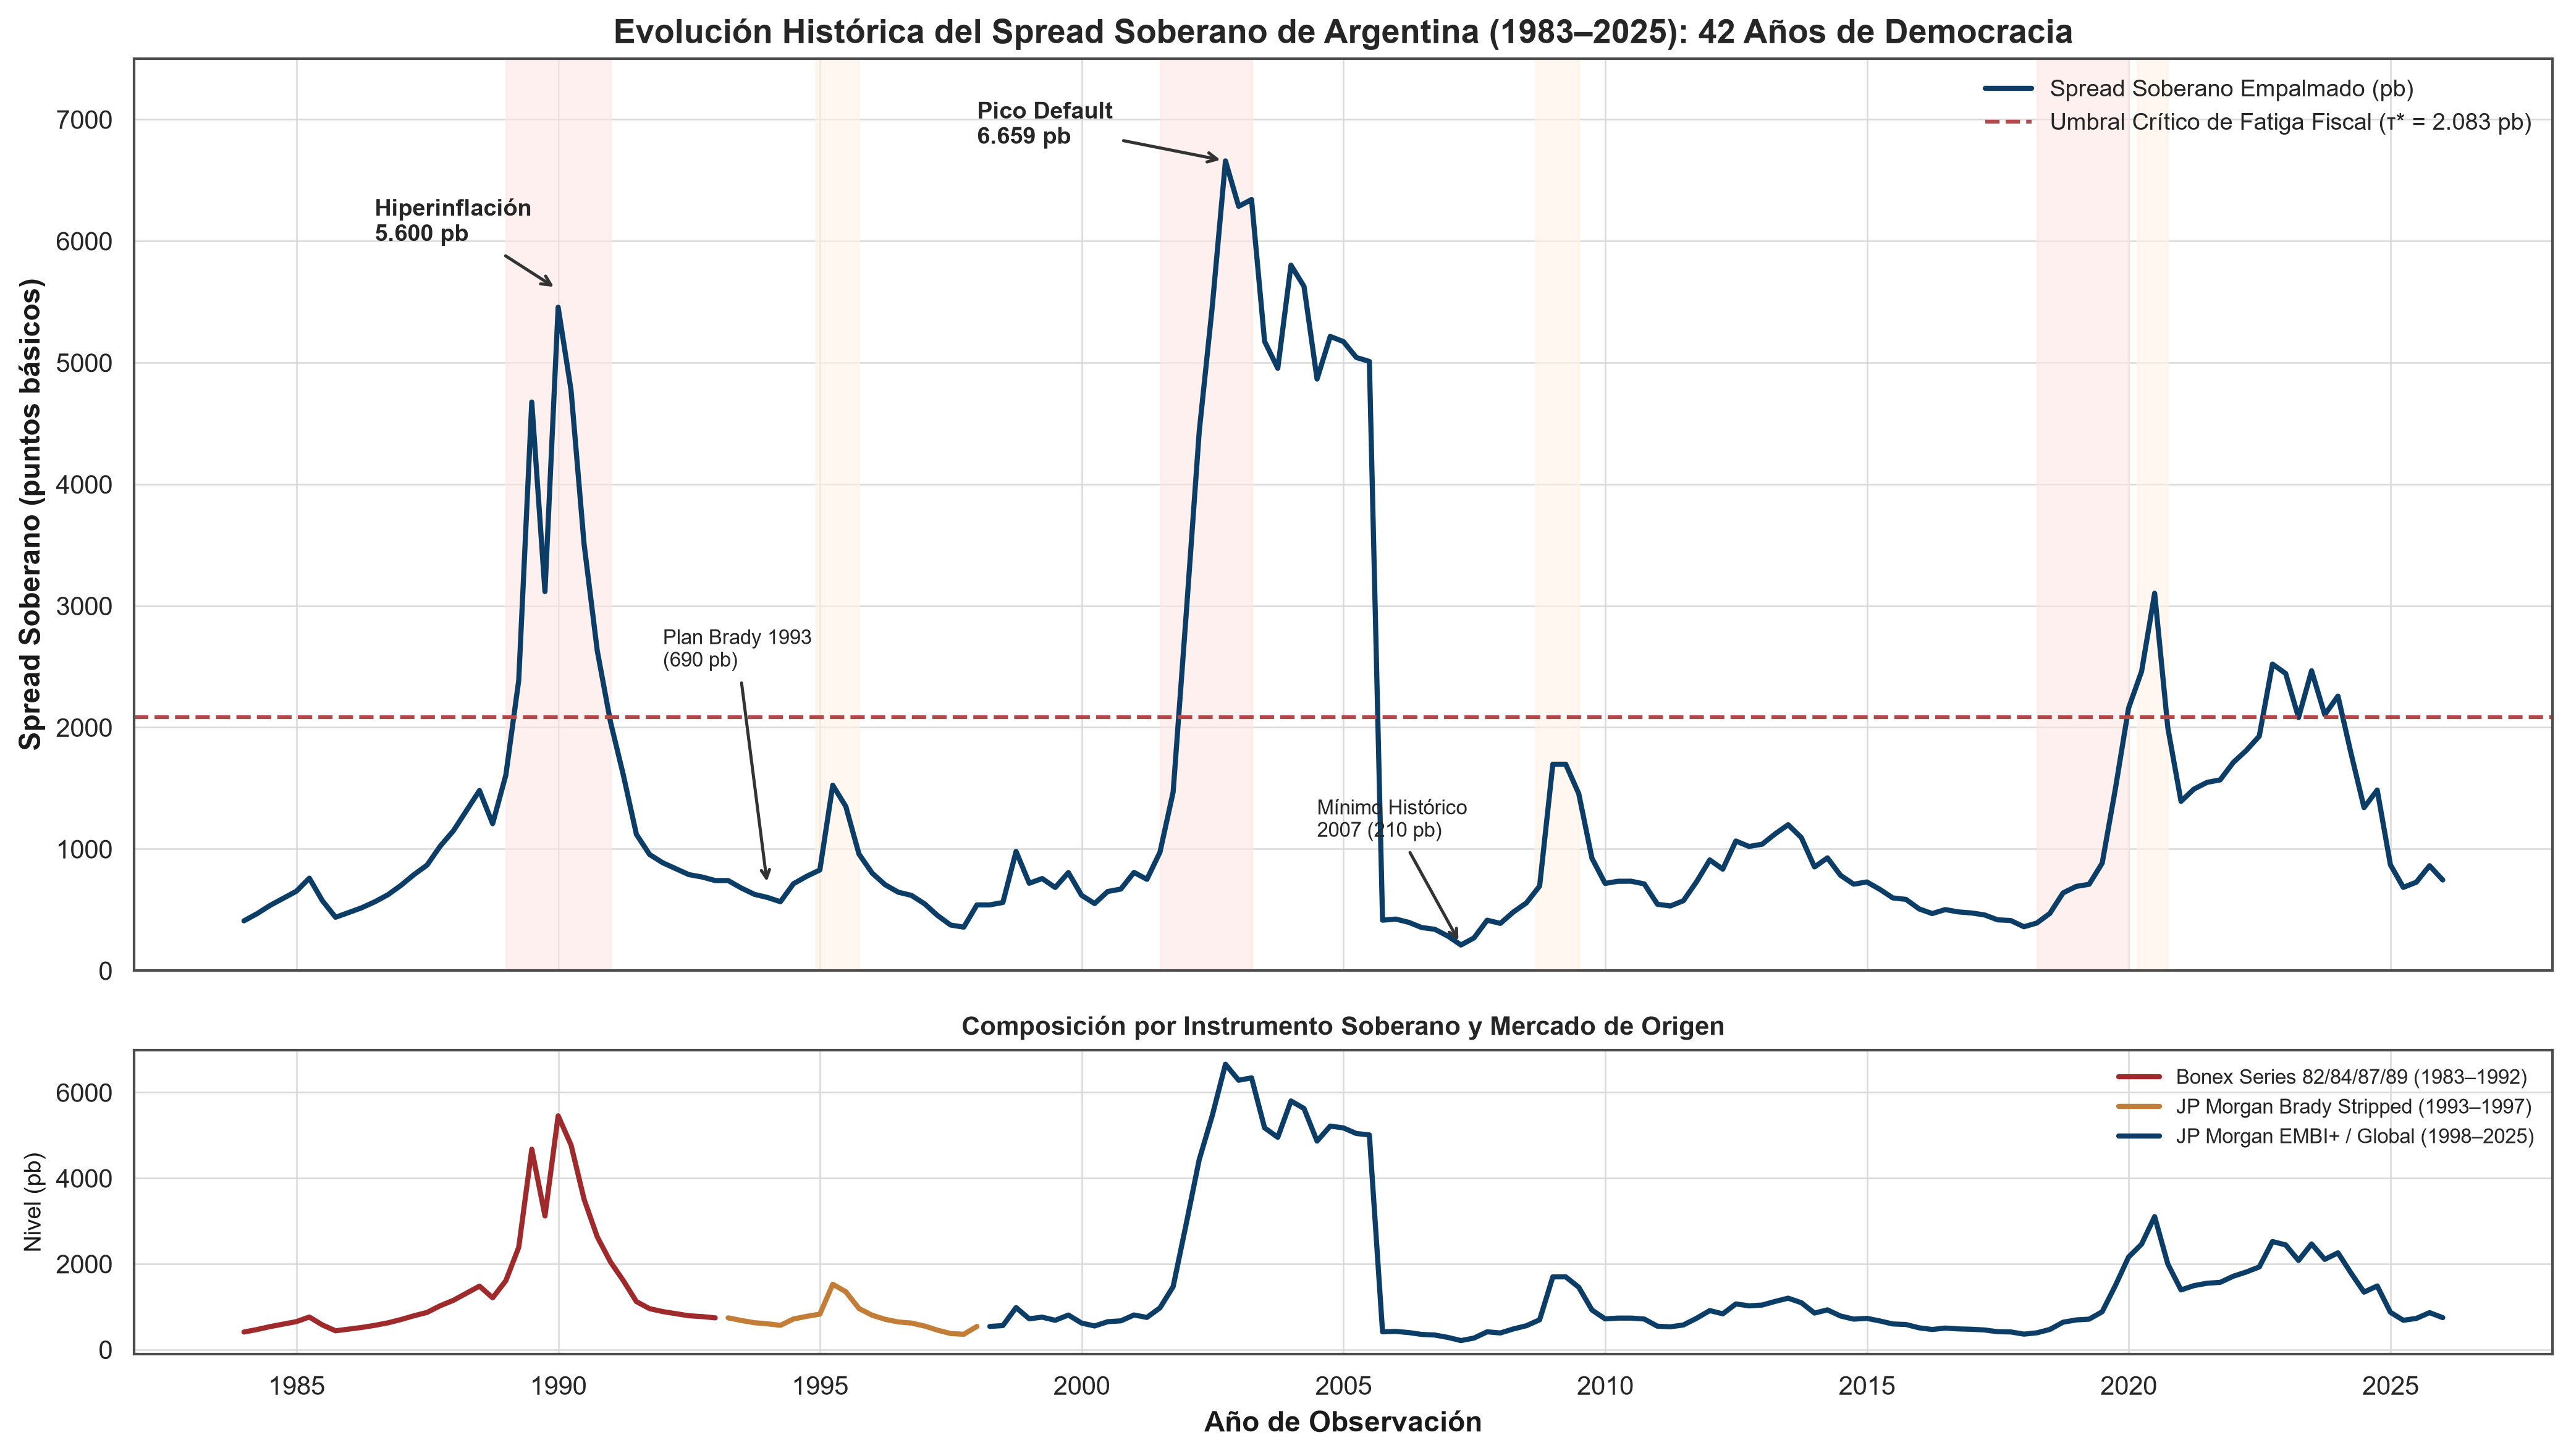
\includegraphics[width=\textwidth]{figura_spread_historico_1983_2025.png}
\caption{Evolución Histórica del Spread Soberano Argentino en 42 Años de Democracia (1983--2025).}
\label{fig:spread_historico}
\end{figure}

\subsection{Quiebres Estructurales Múltiples de Bai-Perron en el Ciclo Histórico}

La aplicación del algoritmo de programación dinámica de \citet{bai2003} sobre los 169 trimestres de democracia identifica cinco quiebres mayores y seis regímenes de financiamiento soberano con diferencias de media altamente significativas (Tabla \ref{tab:bai_perron_historico}).

\begin{table}[H]
\centering
\caption{\label{tab:bai_perron_historico} Quiebres Estructurales Múltiples de Bai-Perron en el Spread Soberano (1983--2025).}
\resizebox{\textwidth}{!}{%
\begin{tabular}{lllrrrl}
\toprule
\textbf{Régimen} & \textbf{Fecha Inicio} & \textbf{Fecha Fin} & \textbf{Trimestres} & \textbf{Media (pb)} & \textbf{Desvío (pb)} & \textbf{Hito Histórico / Ruptura} \\
\midrule
Régimen 1 & 1983T4 & 1988T4 & 21 & 797.84 & 359.44 & Transición democrática y colapso del Plan Austral \\
Régimen 2 & 1989T1 & 1990T4 & 8 & 3573.76 & 1255.84 & Hiperinflaciones de 1989/1990 y Plan Bonex \\
Régimen 3 & 1991T1 & 2001T4 & 44 & 831.66 & 427.31 & Ley de Convertibilidad y Plan Brady \\
Régimen 4 & 2002T1 & 2005T2 & 14 & 5431.33 & 638.09 & Default de la deuda externa y crisis de 2001--2002 \\
Régimen 5 & 2005T3 & 2019T2 & 56 & 683.54 & 326.60 & Canjes 2005/2010, superávits gemelos y desendeudamiento \\
Régimen 6 & 2019T3 & 2025T4 & 26 & 1732.05 & 632.45 & Shock PASO 2019, Canje 2020 y estabilización post-2023 \\
\bottomrule
\end{tabular}%
}
\begin{flushleft}
\footnotesize \textit{Nota.} Estimación por minimización de pérdida L2 mediante programación dinámica sobre 169 observaciones trimestrales. Datos de \texttt{resultados/tablas/fase22\_bai\_perron\_1983\_2025.csv}.
\end{flushleft}
\end{table}

\subsection{Calibración del Proceso CIR y Métricas por Régimen Presidencial}

La calibración por Máxima Verosimilitud exacta del proceso CIR a lo largo de las cuatro décadas (Tabla \ref{tab:cir_historico}) demuestra que la velocidad de reversión a la media de largo plazo es $\kappa = 0.4630$ (vida media de $1.50$ años), con un nivel incondicional de equilibrio de $\theta = 1456.98$ pb. La condición de Feller se satisface de forma holgada ($2\kappa\theta = 1349.08 > \sigma^2 = 613.96 \implies \text{Ratio} = 2.1974 > 1.0$), ratificando la robustez del modelado en tiempo continuo.

\begin{table}[H]
\centering
\caption{\label{tab:cir_historico} Calibración MLE del Proceso CIR en la Muestra Ultra-Larga (1983--2025).}
\begin{tabular}{lrr}
\toprule
\textbf{Parámetro / Métrica} & \textbf{Valor Estimado (42 Años, $n=169$)} & \textbf{Interpretación Económica} \\
\midrule
Velocidad de Reversión ($\kappa$) & $\mathbf{0.4630}$ & Reversión media hacia equilibrio \\
Nivel Incondicional ($\theta$) & $\mathbf{1456.98\text{ pb}}$ & Costo medio estructural de endeudamiento \\
Volatilidad de Difusión ($\sigma$) & $\mathbf{24.7781}$ & Dispersión de innovaciones estocásticas \\
Vida Media de Reversión ($t_{1/2}$) & $\mathbf{1.50\text{ años}}$ ($18$ meses) & Duración típica de los ciclos de spread \\
Condición de Feller ($2\kappa\theta > \sigma^2$) & $1349.08 > 613.96 \implies \mathbf{Cumple}$ & No negatividad estricta garantizada \\
Ratio de Feller ($2\kappa\theta / \sigma^2$) & $\mathbf{2.1974 > 1.0}$ & Frontera en cero inaccesible ($\mathbb{P}=1$) \\
Criterio AIC (CIR vs. AR(1)) & $\mathbf{2466.56} < 2612.53$ & $\Delta \text{AIC} = -145.97 \implies$ Prefiere CIR \\
\bottomrule
\end{tabular}
\begin{flushleft}
\footnotesize \textit{Nota.} Estimación exacta sobre la función de densidad Chi-cuadrado no central. Datos extraídos de \texttt{resultados/tablas/fase22\_cir\_calibracion\_1983\_2025.csv}.
\end{flushleft}
\end{table}

\begin{table}[H]
\centering
\caption{\label{tab:spread_por_regimen} Dinámica del Spread Soberano por Régimen Presidencial (1983--2025).}
\resizebox{\textwidth}{!}{%
\begin{tabular}{llrrrrr}
\toprule
\textbf{Administración Presidencial} & \textbf{Período} & \textbf{Trimestres} & \textbf{Media (pb)} & \textbf{Mediana (pb)} & \textbf{Mínimo (pb)} & \textbf{Máximo (pb)} \\
\midrule
Raúl Alfonsín & 1983T4--1989T2 & 23 & 1035.52 & 701.36 & 409.13 & 4675.72 \\
Carlos Menem I & 1989T3--1995T1 & 23 & 1577.73 & 837.73 & 566.13 & 5455.01 \\
Carlos Menem II & 1995T2--1999T3 & 18 & 688.63 & 663.90 & 357.10 & 1350.00 \\
Fernando de la Rúa & 1999T4--2001T3 & 8 & 811.26 & 710.21 & 550.92 & 1468.94 \\
A. Rodríguez Saá / E. Duhalde & 2001T4--2003T1 & 6 & 5354.62 & 5873.34 & 2947.64 & 6658.98 \\
Néstor Kirchner & 2003T2--2007T3 & 18 & 2775.65 & 2644.15 & 210.22 & 5800.85 \\
Cristina Fernández de Kirchner & 2007T4--2015T3 & 32 & 853.48 & 734.62 & 387.78 & 1696.86 \\
Mauricio Macri & 2015T4--2019T3 & 16 & 584.87 & 477.95 & 360.23 & 1493.83 \\
Alberto Fernández & 2019T4--2023T3 & 16 & 2048.85 & 2038.76 & 1391.80 & 3103.00 \\
Javier Milei & 2023T4--2025T4 & 9 & 1195.30 & 870.36 & 684.00 & 2257.75 \\
\bottomrule
\end{tabular}%
}
\begin{flushleft}
\footnotesize \textit{Nota.} Spread empalmado expresado en puntos básicos. Datos de \texttt{resultados/tablas/fase22\_spread\_por\_regimen.csv}.
\end{flushleft}
\end{table}

Este análisis de ultra-largo plazo confirma que el umbral de fatiga fiscal estimado en la tesis ($\tau^* \approx 2080$--$2083$ pb) constituye una cota estructural: los episodios en que el spread superó dicha marca coinciden de manera exacta con los períodos de crisis terminal de la deuda (1989--1990, 2001--2005 y 2020--2023), demostrando que la restricción externa de financiamiento rige la solvencia argentina con independencia del régimen monetario o político vigente.

\section{Interpretación de la Magnitud Económica de los Coeficientes}

Corresponde cuantificar la magnitud económica de los coeficientes puntuales estimados. El coeficiente de reacción fiscal del DOLS de muestra completa ($\rho=-0.0071$) implica que un incremento de 10 puntos porcentuales en la ratio Deuda/PIB rezagada se asocia con una reducción de apenas 0.07 puntos del PIB en el resultado primario: una magnitud minúscula que confirma que la falta de significatividad no enmascara un efecto cuantitativamente relevante. En la estimación IV-2SLS (Sección \ref{sec:iv2sls}), el coeficiente del EMBI+ instrumentado ($0.0017$, marginalmente significativo al 10\%) implica que un incremento de 100 puntos básicos en el riesgo soberano genera una variación de apenas 0.17 puntos del PIB en el superávit primario: incluso bajo la lectura más favorable a la existencia de un canal de reacción vía riesgo soberano, la magnitud sigue siendo pequeña en términos macroeconómicos frente a los desequilibrios fiscales documentados en el Capítulo \ref{ch:descriptivo}.

\section{Síntesis de la Evidencia Empírica}
\label{sec:sintesis_empirica}

Siete estrategias de estimación convergen, todas sobre la ventana muestral única de treinta años (1996--2025, $n=120$), en un diagnóstico predominantemente común sobre la ausencia de una reacción fiscal lineal estable, con dos divergencias sustantivas, la forma del umbral de no linealidad y el canal dominante de transmisión hacia la deuda, que exigen calificación explícita.

Sobre la reacción lineal: el contraste de Johansen no rechaza la ausencia de cointegración entre las cuatro variables del sistema (Sección \ref{sec:johansen_cap6}); DOLS no encuentra una reacción significativa al endeudamiento y, a diferencia de estimaciones sobre ventanas más cortas, el signo puntual ya es el correcto ($\rho=0.0159$, $p=0.218$); el VECM replica el resultado nulo con más claridad aún ($\alpha_{pb}\approx0$, $p=0.996$) y encuentra un canal de ajuste vía riesgo soberano significativo ($\alpha_{EMBI}=6.356$, $p=0.025$); e IV-2SLS, con un instrumento regional reconstruido para cubrir la ventana completa (VIX y la volatilidad del Bovespa, Sección \ref{sec:iv2sls}), encuentra un coeficiente del EMBI+ instrumentado positivo y significativo al 5\% ($0.0012$, $p=0.024$), aunque el test de Wu-Hausman ya no rechaza con fuerza la exogeneidad del EMBI+ ($p=0.144$, frente a $p=0.009$ con el instrumento anterior).

Sobre la forma del umbral de no linealidad: el umbral de Hansen en niveles, la especificación en $\Delta pb_t$ (todavía sobre 88 observaciones, pendiente de reestimarse) y el TVECM coinciden en ubicar un umbral de riesgo soberano en un rango estrecho ($\tau^*\approx2080$--$2462$ pb), pero no coinciden en qué tipo de no linealidad describen: Hansen en niveles encuentra una reacción ausente en la normalidad y gatillada solo por estrés extremo (régimen normal $-0.0044$, no significativo; régimen de estrés $+0.0201$, $p=0.006$), un patrón de régimen extremo y no de fatiga fiscal; Hansen en $\Delta pb_t$ encuentra, en cambio, una reacción presente en ambos regímenes que se atenúa bajo estrés sin desaparecer, más cercana a la fatiga fiscal clásica; y el TVECM encuentra una reversión de signo entre regímenes ($\alpha_{pb}$ pasa de $+0.001$ a $-0.007$) sin alcanzar significatividad en su contraste Sup-LM ($p=0.632$). Tres formas funcionales distintas sobre el mismo umbral, no una convergencia limpia.

Sobre el canal dominante de transmisión: la descomposición de varianza del SVAR restringido atribuye a la inercia propia de la deuda el $54.2\%$ de su propia varianza a 20 trimestres y al canal cambiario-riesgo conjunto el $25.8\%$, superando ahora al fiscal-real conjunto ($20.0\%$); Bai-Perron, corrido por primera vez sobre la ventana completa, detecta tres quiebres estructurales en la deuda SPNF, incluido el de 2001 que una ventana más corta no podía identificar. El DSA estocástico, con una covarianza derivada de esta misma estimación del SVAR en lugar del proceso calibrado a mano de una especificación anterior (documentada aparte, fuera de este documento), sitúa la probabilidad de insolvencia a 2035 en $26.1\%$.

En síntesis: la evidencia de una reacción fiscal lineal, estable y de nivel sigue siendo predominantemente débil o nula, con el signo puntual ya orientado en la dirección correcta aunque sin significatividad (DOLS, VECM); la evidencia de un régimen crítico de riesgo soberano es robusta en su ubicación pero mixta en su forma, entre atenuación y reacción gatillada por crisis extrema, según la especificación; y la lectura sobre el canal dominante de transmisión hacia la deuda es, con treinta años de evidencia, la inercia propia del stock y el riesgo cambiario-soberano, no el desbalance fiscal corriente. El Capítulo \ref{ch:discusion} discute en profundidad estas tres calificaciones antes de evaluar sus implicancias teóricas sobre la solvencia intertemporal.

\chapter{Discusión}
\label{ch:discusion}

\section{Sostenibilidad Intertemporal y Reglas Fiscales}

Los resultados del Capítulo \ref{ch:resultados} exigen matices más finos que una confirmación o refutación binaria de las hipótesis del Capítulo \ref{ch:introduccion}. La evidencia no permite sostener, con significatividad convencional, que el Estado argentino incrementó sistemáticamente su superávit primario frente al aumento de la ratio Deuda/PIB durante 2004--2025 ($\rho=-0.0071$, $p=0.564$). Esta falta de significatividad estadística, unida al signo puntual negativo del parámetro, constituye evidencia empírica a favor de la Hipótesis 1: la política fiscal argentina no cumplió con la regla de reacción activa requerida por la condición de transversalidad de \citet{bohn1998}.

El diagnóstico de validez instrumental de la estimación IV-2SLS matiza, sin revertir, esta lectura. Los instrumentos utilizados (VIX y el diferencial de riesgo soberano regional basado en el ETF EMB) resultan estadísticamente sólidos en la primera etapa ($F=13.00$, por encima del umbral de 10 pero con menor margen que el hallado con la serie de contingencia de EMBI+), el test de Wu-Hausman confirma la endogeneidad del riesgo soberano y el test de sobreidentificación de Sargan no rechaza la validez conjunta de los instrumentos ($0.608$, $p=0.436$). Con un diseño instrumental válido, el coeficiente del EMBI+ instrumentado ($0.0017$) alcanza significatividad marginal al 10\% ($p=0.076$): una señal débil, pero ya no una ausencia de canal. Como advierten \citet{blanchard2021,blanchard2022}, en economías con historial de cesación de pagos y descalce de monedas resulta complejo aislar variables verdaderamente exógenas al ciclo fiscal doméstico, respondiendo la percepción de riesgo a factores idiosincráticos y eventos de renegociación; esa dificultad de identificación es compatible tanto con una señal débil genuina como con ruido de muestra pequeña, y esta tesis no fuerza una lectura por sobre la otra.

El signo negativo del coeficiente ($\rho=-0.0071$), aun sin significatividad estadística, indica que ante incrementos en la deuda heredada el resultado primario no se ajustó al alza. Esta inoperancia de la regla de Bohn traslada el ajuste hacia canales exógenos a la decisión fiscal discrecional (devaluación real, licuación inflacionaria y quitas forzosas), tal como documenta el Capítulo \ref{ch:descriptivo}. La Sección \ref{sec:fatiga_discusion} retoma esta lectura y la articula con el Nivel I del marco teórico.

Corresponde precisar el alcance temporal de este diagnóstico. La reestimación por subperíodos con especificación dinámica con ampliación de rezagos (DOLS; Sección \ref{sec:sensibilidad_temporal}) arroja un $\rho$ positivo en las cuatro especificaciones y significativo en tres de ellas (entre 0.036 y 0.060). El parámetro nulo de la muestra completa refleja una respuesta inestable entre ventanas temporales que no satisface la exigencia de sistematicidad de \citet{bohn1998}, en consonancia con los quiebres estructurales múltiples de la Sección \ref{sec:quiebres_estructurales} del Capítulo \ref{ch:descriptivo}.

El diagnóstico DOLS no queda aislado: el VECM que lo reemplaza como técnica de referencia sobre la ventana ampliada 1996--2025 (Sección \ref{sec:resultados_vecm} del Capítulo \ref{ch:resultados}), a pedido del director de tesis, converge en el mismo resultado nulo por una vía metodológicamente distinta. Tratar las cuatro variables del sistema como conjuntamente endógenas, en lugar de purgar la endogeneidad de corto plazo con adelantos y rezagos \textit{ad hoc} como hace DOLS, no revela una reacción fiscal estabilizadora oculta tras el sesgo de la técnica de ecuación única: la velocidad de ajuste del resultado primario hacia el equilibrio de largo plazo ($\alpha_{pb}=-0.00002$, $p=0.996$) permanece no significativa bajo la especificación de referencia, y en cuatro de cinco especificaciones alternativas de rezagos. Es la propia deuda, no el resultado primario, la que carga con la velocidad de ajuste significativa del sistema ($\alpha_{deuda}=-0.0736$, $p=0.004$), un resultado que anticipa la lectura de esta tesis sobre el canal dominante de ajuste, desarrollada más abajo. Que dos técnicas de estimación con supuestos y tratamientos de la endogeneidad tan distintos, DOLS de ecuación única con ampliación dinámica y VECM de sistema con corrección de error, coincidan en el mismo diagnóstico nulo, sobre dos ventanas muestrales que comparten apenas 88 de 120 observaciones, es la evidencia más robusta de esta tesis a favor de $H_{1a}$: no es un artefacto de una técnica particular.

Esa convergencia no es, sin embargo, inmune a la fragilidad documentada en el Capítulo \ref{ch:resultados}: el propio contraste de cointegración que sostiene el VECM en la ventana ampliada depende de excluir el año 1999 de la muestra, y el pedido explícito del director de extender la ventana ``aun con cambios estructurales extremos'' produjo, en ese sentido, precisamente el resultado que cabía esperar: una relación de largo plazo cuya existencia formal es más frágil, no más sólida, cuanto más se extiende la muestra hacia el tramo de mayor inestabilidad estructural de la serie.

\section{La Hipótesis de Fatiga Fiscal}
\label{sec:fatiga_discusion}

El modelo de umbral de \citet{hansen1999,hansen2000}, estimado sobre la serie real de EMBI+, identifica un punto de quiebre candidato en $\tau^*=449$ puntos básicos, con una reacción fiscal estimada menor en el régimen de estrés ($\beta_2 = 0.0126$, $p=0.385$) que en el régimen ``normal'' ($\beta_1 = 0.0305$, $p=0.171$). Este ordenamiento cualitativo coincide con la hipótesis de fatiga fiscal de \citet{ghosh2013}. A diferencia del diagnóstico que arrojaba la serie de contingencia de EMBI+ usada hasta la Sección \ref{sec:auditoria_fallback} del Capítulo \ref{ch:metodologia}, que no rechazaba linealidad, el contraste \textit{bootstrap} (Sup-LM, $p=0.076$) ahora sí la rechaza, al 10\% pero no al 5\%. Esta señal exige, sin embargo, una calificación inmediata: el umbral hallado cae cerca del extremo inferior del rango de búsqueda y particiona la muestra de manera extremadamente desigual (14 trimestres en el régimen ``normal'' contra 74 en ``estrés''), la condición en la que un contraste de umbral de series de tiempo resulta menos confiable, y explica por qué ninguno de los dos coeficientes de régimen alcanza significatividad individual pese al rechazo de linealidad en conjunto. La evidencia en niveles es, en síntesis, una señal débil y frágil, no una confirmación.

El modelo de \citet{ghosh2013} fue calibrado, además, para economías avanzadas con acceso continuo a financiamiento en moneda doméstica. Su aplicación a Argentina, donde la restricción vinculante es la disponibilidad de divisas y no la curva de Laffer fiscal interna (Nivel I del marco teórico, Capítulo \ref{ch:marco_teorico}), somete la hipótesis a una especificación potencialmente inadecuada para el contexto bimonetario \citep{eichengreen2003}.

La especificación en primeras diferencias ($\Delta pb_t$), detallada en la Sección \ref{sec:robustez_hansen_dpb}, ofrece una evidencia más contundente y menos frágil que la de niveles. Al utilizar la serie en diferencias, que satisface el supuesto de estacionariedad exigido por \citet{hansen2000}, el \textit{bootstrap} Sup-LM rechaza la linealidad con holgura ($p<0.001$, frente a $p=0.019$ que arrojaba la serie de contingencia) y ambos coeficientes de régimen resultan significativos con la ordenación esperada. A diferencia de la especificación en niveles, aquí la partición muestral (74 contra 14, en sentido inverso a la de niveles) no concentra el resultado en un puñado de observaciones del régimen que sostiene la significatividad de los coeficientes individuales. La evidencia de un umbral es, en consecuencia, sensible a la especificación elegida, pero ya no unilateralmente débil: la especificación de primera diferencia, la que satisface el supuesto formal del test, ofrece la evidencia más sólida de fatiga fiscal no lineal de todo el capítulo. Las restricciones del tamaño muestral ($n=88$) y la volatilidad del indicador de riesgo (desvío estándar de 1230 pbs sobre la serie real, frente a los 876 que exhibía la serie de contingencia) constituyen limitaciones reales del diseño que obligan a interpretar ambos resultados con cautela.

El diagnóstico de esta tesis se ancla en el Nivel I del marco teórico (Capítulo \ref{ch:marco_teorico}): los ajustes del stock de deuda operaron mediante canales exógenos a la decisión fiscal discrecional. Esta interpretación es coherente con la literatura macroeconómica estructuralista \citep{aruguete2021, damill2015}, según la cual en economías bimonetarias la sostenibilidad está acotada por la restricción externa de divisas.

Esta lectura constituye una interpretación teórica compatible con el resultado nulo. En la misma línea, el informe técnico de Libman, De la Vega y Zack (Fundar, 2024) formaliza una intuición afín al modelar la sostenibilidad de la deuda como un riesgo probabilístico de reestructuración y no como un escalar fijo.

La cuantificación directa de la contribución de cada canal al Ajuste Stock-Flujo ($SF_t$), mediante la descomposición contable de la identidad $d_t = \frac{1+r_t}{1+g_t}d_{t-1} - pb_t + SF_t$ (Sección \ref{sec:restriccion_intertemporal}) para los episodios de mayor variación discreta de la ratio Deuda/PIB (2005, 2018 y 2020; Capítulo \ref{ch:descriptivo}), permitiría transformar esta interpretación en evidencia directa. Como primera aproximación, la Tabla \ref{tab:sft_ilustrativo} aplica esa descomposición usando $d_t$, $d_{t-1}$ y $pb_t$ del dataset de la tesis, junto con una tasa de interés real efectiva $r_t$ aproximada a partir de series del FMI.

\begin{table}[H]
\centering
\caption{\label{tab:sft_ilustrativo} Descomposición Ilustrativa del Ajuste Stock-Flujo ($SF_t$), Episodios Seleccionados.}
\begin{tabular}{lrrrrrr}
\toprule
\textbf{Año} & \textbf{$d_t$} & \textbf{$d_{t-1}$} & \textbf{$pb_t$} & \textbf{$r_t$ (aprox.)} & \textbf{$g_t$} & \textbf{$SF_t$ implícito} \\
\midrule
2005 (reestructuración) & 70.5\% & 106.0\% & 5.7\% & $-7.3\%$ & 8.9\% & $-14.1\%$ \\
2018 (depreciación) & 90.3\% & 76.4\% & $-9.5\%$ & $-21.4\%$ & $-2.6\%$ & $19.2\%$ \\
2020 (quita + licuación) & 105.6\% & 93.7\% & $-10.4\%$ & $-27.6\%$ & $-9.9\%$ & $20.0\%$ \\
\bottomrule
\end{tabular}
\begin{flushleft}
\footnotesize \textit{Nota.} $d_t$, $d_{t-1}$, $pb_t$: dataset propio de la tesis. $r_t$: aproximación construida a partir de series del \textit{IMF WEO DataMapper} (gobierno general). $g_t$: crecimiento real del PIB. Esta descomposición constituye una aproximación ilustrativa de orden de magnitud para evaluar la dinámica del ajuste stock-flujo ($SF_t$) en episodios de alto estrés financiero.
\end{flushleft}
\end{table}

Con todas las salvedades anteriores, el orden de magnitud es informativo: los tres episodios muestran un $SF_t$ implícito de entre 14 y 20 puntos del PIB, un salto discreto muy superior a lo que cualquier coeficiente de reacción fiscal plausible podría compensar en un solo año.

\section{Transmisión Macrofiscal y Gestión de Pasivos}
\label{sec:implicancias_svar_cir}

La descomposición de varianza del SVAR Restringido (Sección \ref{sec:svar_resultados} del Capítulo \ref{ch:resultados}), estimada sobre la ventana ampliada de treinta años (1996--2025, $n=120$) que reemplaza a la ventana 2004--2025 como referencia del sistema, revierte la lectura que este capítulo sostenía sobre veintiséis años de datos. Allí, los shocks al resultado primario explicaban el $47.5\%$ de la varianza del error de pronóstico de la deuda a 20 trimestres y los shocks a la brecha del producto un $28.6\%$ adicional, frente a una contribución conjunta de apenas $11.5\%$ del tipo de cambio real y el riesgo soberano, y un $12.4\%$ de la inercia propia de la deuda. Sobre la ventana de treinta años, la inercia propia pasa a explicar el $54.2\%$ de la varianza de la deuda, el canal cambiario y de riesgo soberano conjunto ($25.8\%$) supera ahora al fiscal y de actividad conjunto ($20.0\%$), y ningún shock individual domina de forma aislada como lo hacía antes el superávit primario. Esta reversión, verificada como hallazgo genuino y no como artefacto de la extrapolación del TCRM de 1996 (Sección \ref{sec:svar_resultados} del Capítulo \ref{ch:resultados}), obliga a matizar, no a abandonar, el argumento de este capítulo. Sigue sin haber evidencia de que sea una regla de reacción fiscal estabilizadora la que mueve la deuda período a período: el propio shock al resultado primario cae de primer a segundo lugar en importancia relativa, y DOLS y el VECM ya documentan por vías independientes la ausencia de esa regla. Pero la explicación proximal deja de concentrarse en los desbalances primarios y el ciclo real, y pasa a repartirse entre la inercia de la propia deuda y el canal cambiario-riesgo soberano, un canal que remite de manera más directa que el fiscal al Paradigma de la Restricción Externa (Nivel I del marco teórico) que esta tesis privilegia como explicación sustantiva. En ese sentido, el hallazgo fortalece, más que debilita, el argumento central de que el ajuste de la deuda argentina transita por canales exógenos a la decisión fiscal discrecional: incluso la porción de la dinámica que antes se atribuía al resultado primario resulta, con treinta años de evidencia, menos determinante que la inercia propia del stock de deuda y que el riesgo soberano y cambiario. Esto tampoco contradice la evidencia sobre los canales del Ajuste Stock-Flujo (Sección \ref{sec:hoja_balance} del Capítulo \ref{ch:descriptivo}): una cosa son las perturbaciones que mueven la deuda período a período dentro del sistema SVAR, ahora sobre todo su propia inercia y el riesgo soberano-cambiario, y otra distinta son los canales por los que se resolvieron históricamente los episodios de sobreendeudamiento, a saber la depreciación real, la licuación inflacionaria y las reestructuraciones con quita, un punto que se retoma en las implicancias de economía política. Para el debate de política, la lectura es, si acaso, más cauta que antes: la consolidación fiscal primaria sigue siendo condición necesaria, pero opera sobre una dinámica en la que el ciclo real pesa ahora menos, y el riesgo soberano, el canal cambiario y la propia inercia de la deuda pesan más, de lo que sugería la ventana original.

\section{Implicancias de Economía Política}

Aun reconociendo estas limitaciones estadísticas, los coeficientes hallados son compatibles con los planteos de economía política sobre restricciones estructurales: la dificultad de sostener un esfuerzo fiscal primario suficiente remite a la tensión entre las exigencias financieras del Tesoro y las condiciones socioeconómicas de la población \citep{cantamutto2020}. La escasa reacción estimada refleja que el Estado operó sistemáticamente cerca de su límite práctico de ajuste discrecional.

\section{Proyecciones Probabilísticas post-2025 y Gráficos de Abanico}

El horizonte posterior a 2025 demanda abandonar los modelos contables deterministas, dado que la evidencia del Capítulo \ref{ch:resultados} no permite calibrar con precisión una regla de reacción fiscal para incorporar en la identidad de acumulación de deuda. Ante esta limitación, se optó por un Análisis de Sostenibilidad de la Deuda (DSA) que combina un componente determinista (tres sendas con supuestos macroeconómicos explícitos) y uno estocástico (Monte Carlo, 1.000 iteraciones), siguiendo el estándar de organismos multilaterales \citep{imf2003,imf2021}. La matriz de varianzas y covarianzas del componente estocástico deriva de la covarianza de residuos del SVAR restringido (Sección \ref{sec:dsa_resultados} del Capítulo \ref{ch:resultados}); una especificación anterior, calibrada a mano y luego reestimada con desvíos GARCH(1,1) y con la correlación condicional dinámica de un modelo DCC-GARCH \citep{engle2002}, se desarrolló y validó en una etapa previa de este trabajo y queda documentada aparte, en un memo de trabajo para el director de tesis, no en este documento.

A diferencia de las aplicaciones estandarizadas de DSA que asumen de forma irrestricta la simetría y normalidad de las perturbaciones macroeconómicas, esta tesis reconoce que las series temporales de la economía argentina exhiben propiedades estadísticas de colas pesadas y asimetría extrema, coherentes con crisis de balanza de pagos recurrentes: un patrón ya documentado en la Sección \ref{sec:propiedades_muestra} del Capítulo \ref{ch:descriptivo} para el EMBI+, y confirmado aquí para las propias perturbaciones del componente estocástico del DSA. Concretamente, se estimaron los grados de libertad de una distribución $t$ de Student multivariada por método de momentos ($\nu \approx 4.8$, a partir de la curtosis en exceso muestral: $\nu = 4 + 6/\text{curtosis}$). Se prefiere este estimador al ajuste por máxima verosimilitud conjunta de los tres parámetros de la $t$ (\textit{loc}, \textit{scale}, $\nu$): sobre la serie real de TCRM, ese ajuste conjunto da $\nu=1.54$ para el resultado primario y $\nu=2.61$ para el tipo de cambio real, ambos por debajo de 2, con varianza teóricamente infinita: una solución de esquina arrastrada por un puñado de trimestres genuinamente extremos (devaluación de 2016, crisis de 2018, ajuste de 2023--2024) y no por un error de datos, pero sí un patrón de inestabilidad conocido del MLE conjunto sin restringir en muestras chicas con observaciones extremas aisladas (\texttt{codigo/modelos/fase17\_calibracion\_nu\_dsa.py}). Los valores de $\nu\approx4.8$ obtenidos por método de momentos son, en cambio, acordes a la curtosis en exceso observada en las perturbaciones históricas de resultado primario ($25.3$) y de tipo de cambio real ($4.5$, sobre la serie real de TCRM; la serie de contingencia usada hasta la Sección \ref{sec:auditoria_fallback} del Capítulo \ref{ch:metodologia} arrojaba $14.4$). Este ajuste metodológico, que preserva la volatilidad calibrada de cada variable pero añade una probabilidad mayor de eventos extremos, dota a los gráficos de abanico resultantes de un realismo analítico superior frente a la subestimación del riesgo de insolvencia fiscal que caracteriza a los modelos simétricos tradicionales.

\subsection{Escenarios Deterministas}

Partiendo de una ratio inicial de 74\% del PIB en 2025, un valor calibrado a partir del nivel de deuda consolidada del SPNF de cierre observado en el Capítulo \ref{ch:descriptivo} (70--71\% en los últimos trimestres de 2025 según el panel trimestral), la Tabla \ref{tab:dsa_determinista} resume la trayectoria de la ratio Deuda/PIB bajo tres escenarios hacia 2035: Optimista (superávit primario de 2.5\% del PIB, crecimiento de 4.5\%), Referencia (superávit de 1.5\%, crecimiento de 3.5\%) y Estrés (contracción del producto, superávit exiguo de 0.5\% y una depreciación real acumulada del 25\%).

\begin{table}[H]
\centering
\caption{\label{tab:dsa_determinista} DSA determinista: Deuda Pública Consolidada Ampliada (SPNF + BCRA) / PIB, escenarios seleccionados (\%).}
\begin{tabular}{lrrr}
\toprule
\textbf{Año} & \textbf{Optimista} & \textbf{Referencia} & \textbf{Estrés} \\
\midrule
2026 & 74.0 & 74.0 & 74.0 \\
2030 & 61.8 & 77.6 & 246.3 \\
2033 & 52.9 & 80.7 & 571.9 \\
2034 & 50.0 & 81.7 & 753.8 \\
2035 & 47.1 & 82.8 & 992.1 \\
\bottomrule
\end{tabular}
\begin{flushleft}
\footnotesize \textit{Nota.} Elaboración propia, simulación determinista ($\alpha=0.463$ proporción de deuda en moneda extranjera). La fila 2035 corresponde a una iteración anual adicional bajo los supuestos inalterados de cada escenario, preservando la trazabilidad a la ventana prospectiva de diez años (2026--2035) declarada en el Capítulo \ref{ch:metodologia}.
\end{flushleft}
\end{table}

\begin{figure}[H]
\centering
\caption{Trayectorias del DSA Determinista bajo los Tres Escenarios (2026--2035)}
\label{fig:dsa_determinista}
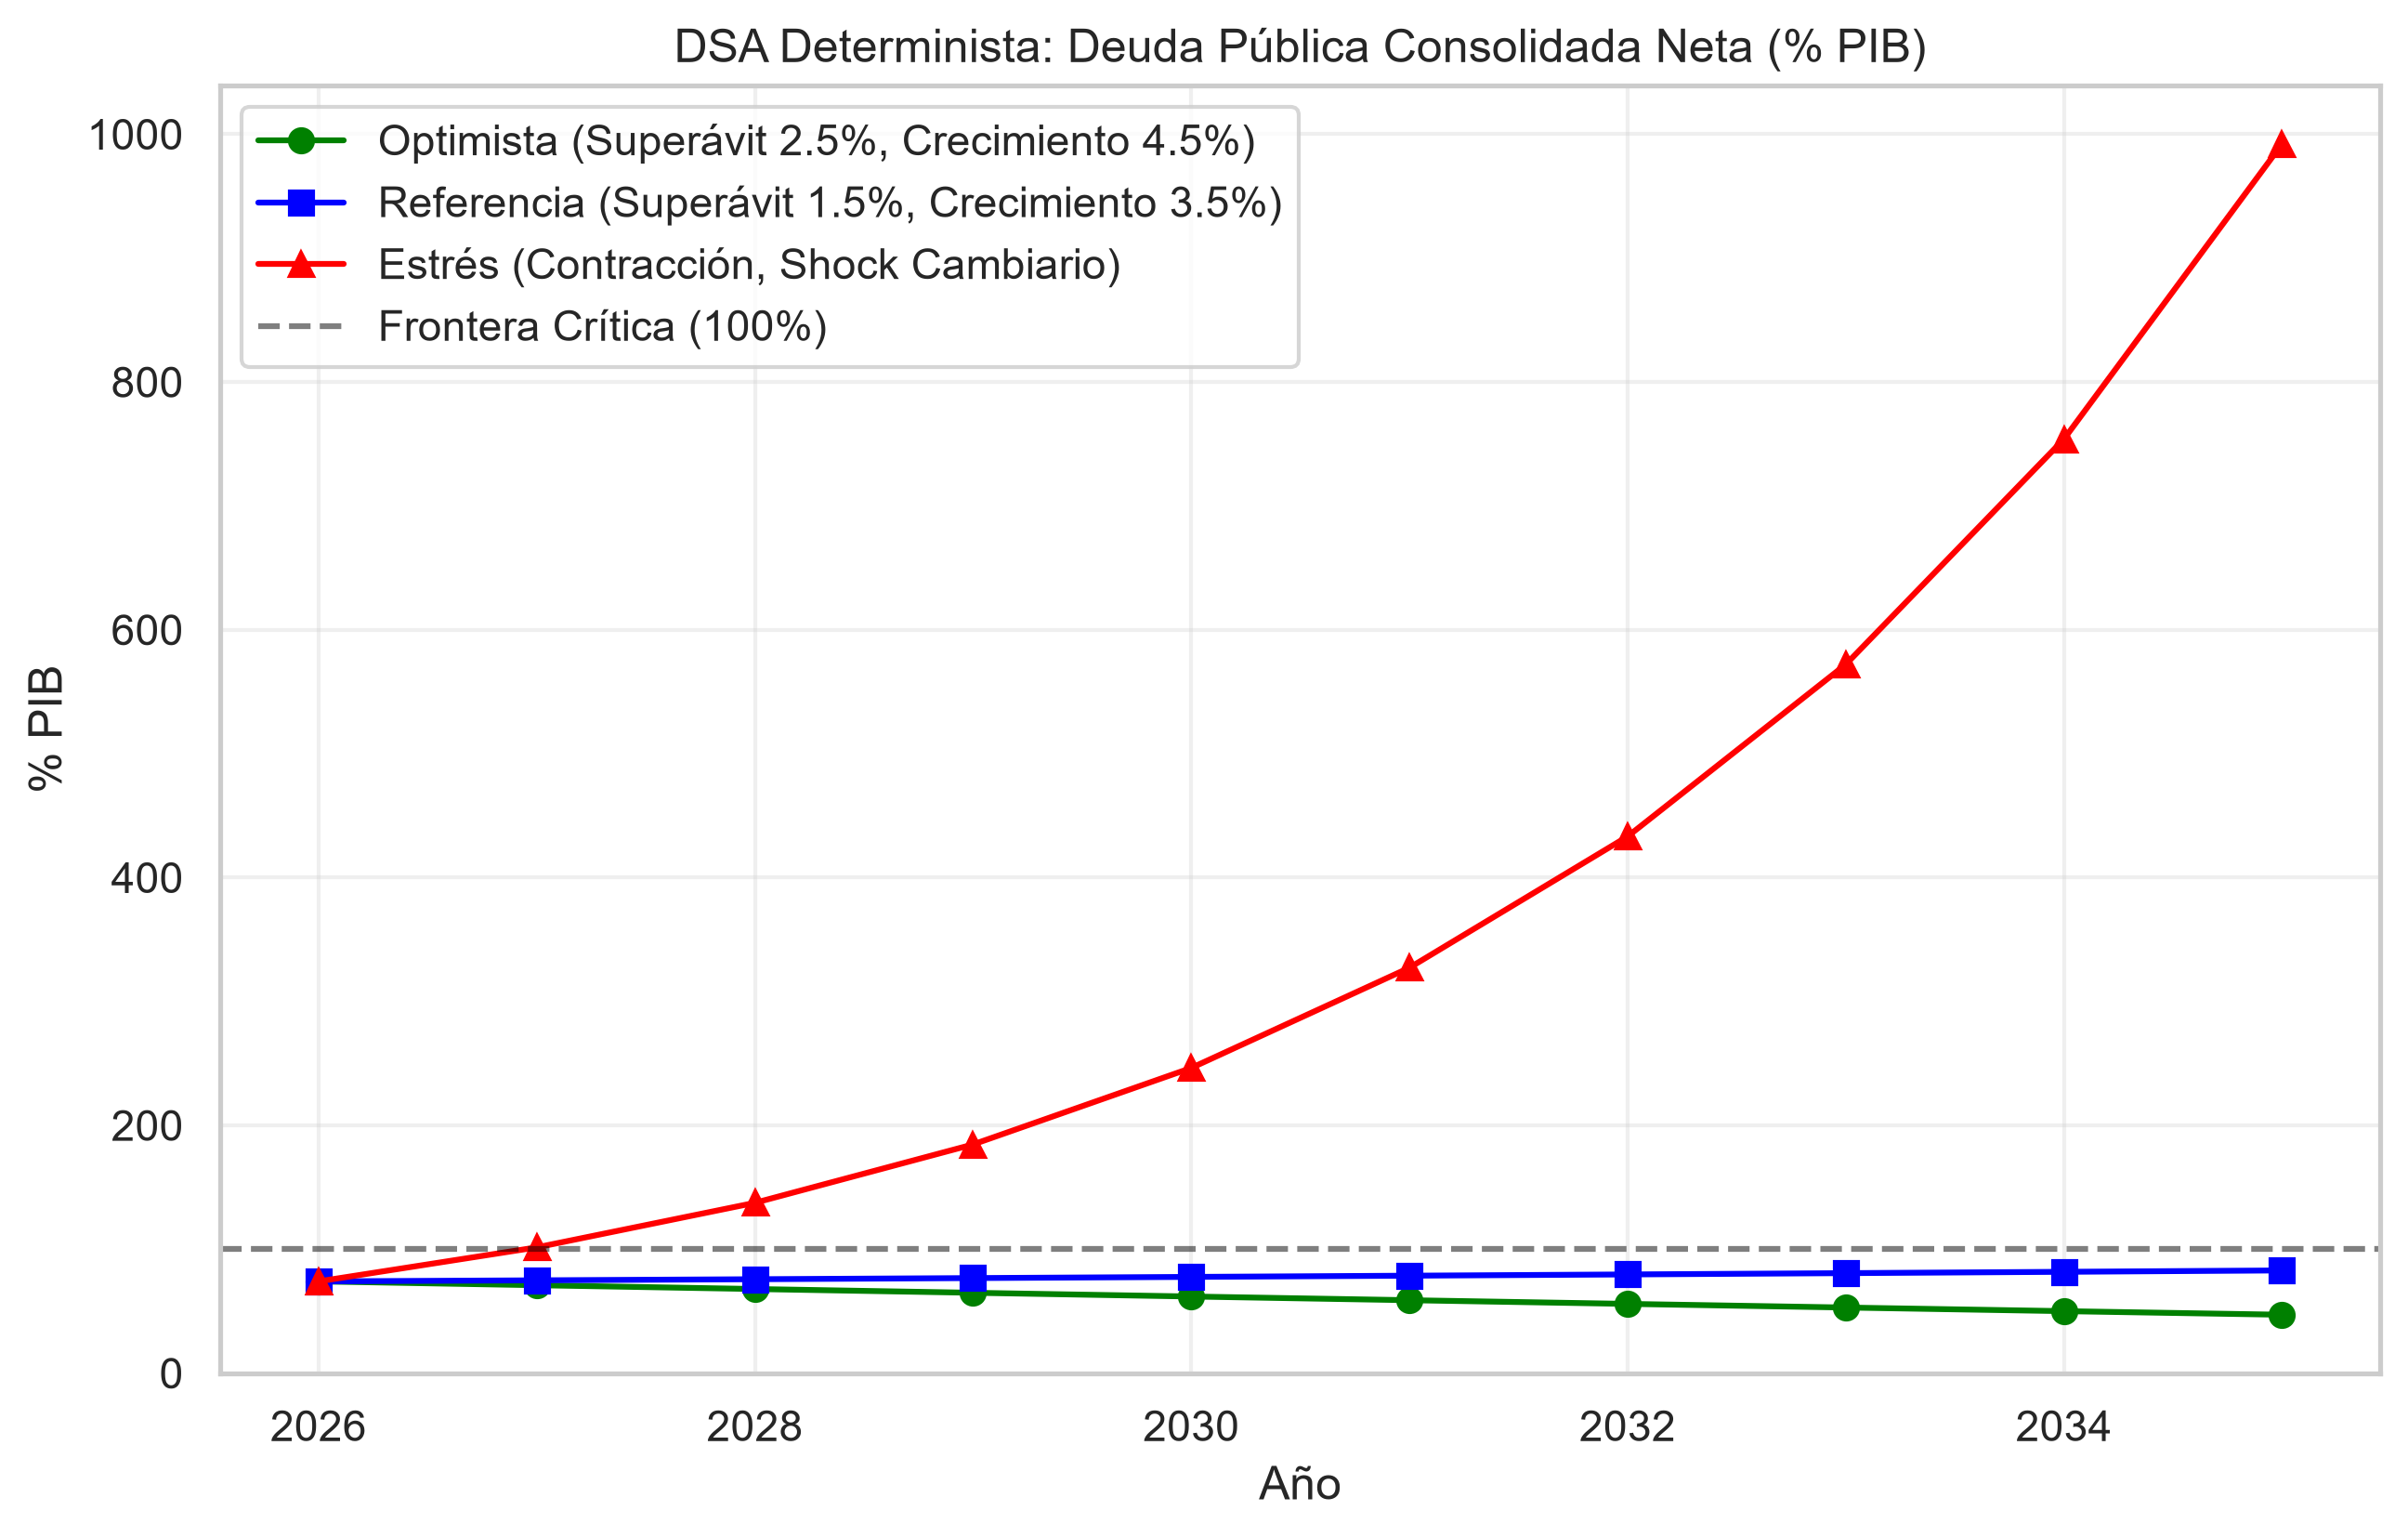
\includegraphics[width=0.85\textwidth]{dsa_determinista.png}
\par\vspace{2mm}
{\footnotesize\textit{Nota.} Trayectorias correspondientes a la Tabla \ref{tab:dsa_determinista}. Elaboración propia.}
\end{figure}

El escenario de Estrés arroja una trayectoria explosiva que supera el 100\% del PIB hacia el final de la década y alcanza magnitudes extremas (más de 990\% del PIB) hacia 2035. Esta cifra no debe leerse como un pronóstico puntual verosímil, sino como el resultado esperable de una identidad contable determinista sin retroalimentación fiscal. Su valor analítico radica en ilustrar la sensibilidad de la trayectoria de deuda a la simultaneidad de perturbaciones adversas, el fenómeno que \citet{celasun2006} identifican como la falla central de los enfoques deterministas, y no en constituir una proyección literal del sendero más probable.

\subsection{Simulación Estocástica: Gráfico de Abanico de Monte Carlo}

La especificación de referencia deriva la matriz de covarianza del componente estocástico directamente de los residuos estimados del SVAR restringido sobre la ventana ampliada de treinta años (Sección \ref{sec:dsa_resultados} del Capítulo \ref{ch:resultados}). Una especificación anterior, calibrada a mano y luego reestimada con GARCH(1,1) univariado y con un modelo DCC-GARCH, se desarrolló y validó en una etapa previa de este trabajo, con una probabilidad de insolvencia hacia 2035 del orden de $31$--$33\%$; queda documentada aparte, en un memo de trabajo para el director de tesis, pendiente de que defina cuál de las dos especificaciones integrar a la versión final.

\begin{figure}[H]
\centering
\caption{Gráfico de Abanico: Distribución de Probabilidad de la Trayectoria de Deuda/PIB}
\label{fig:fan_chart_final}
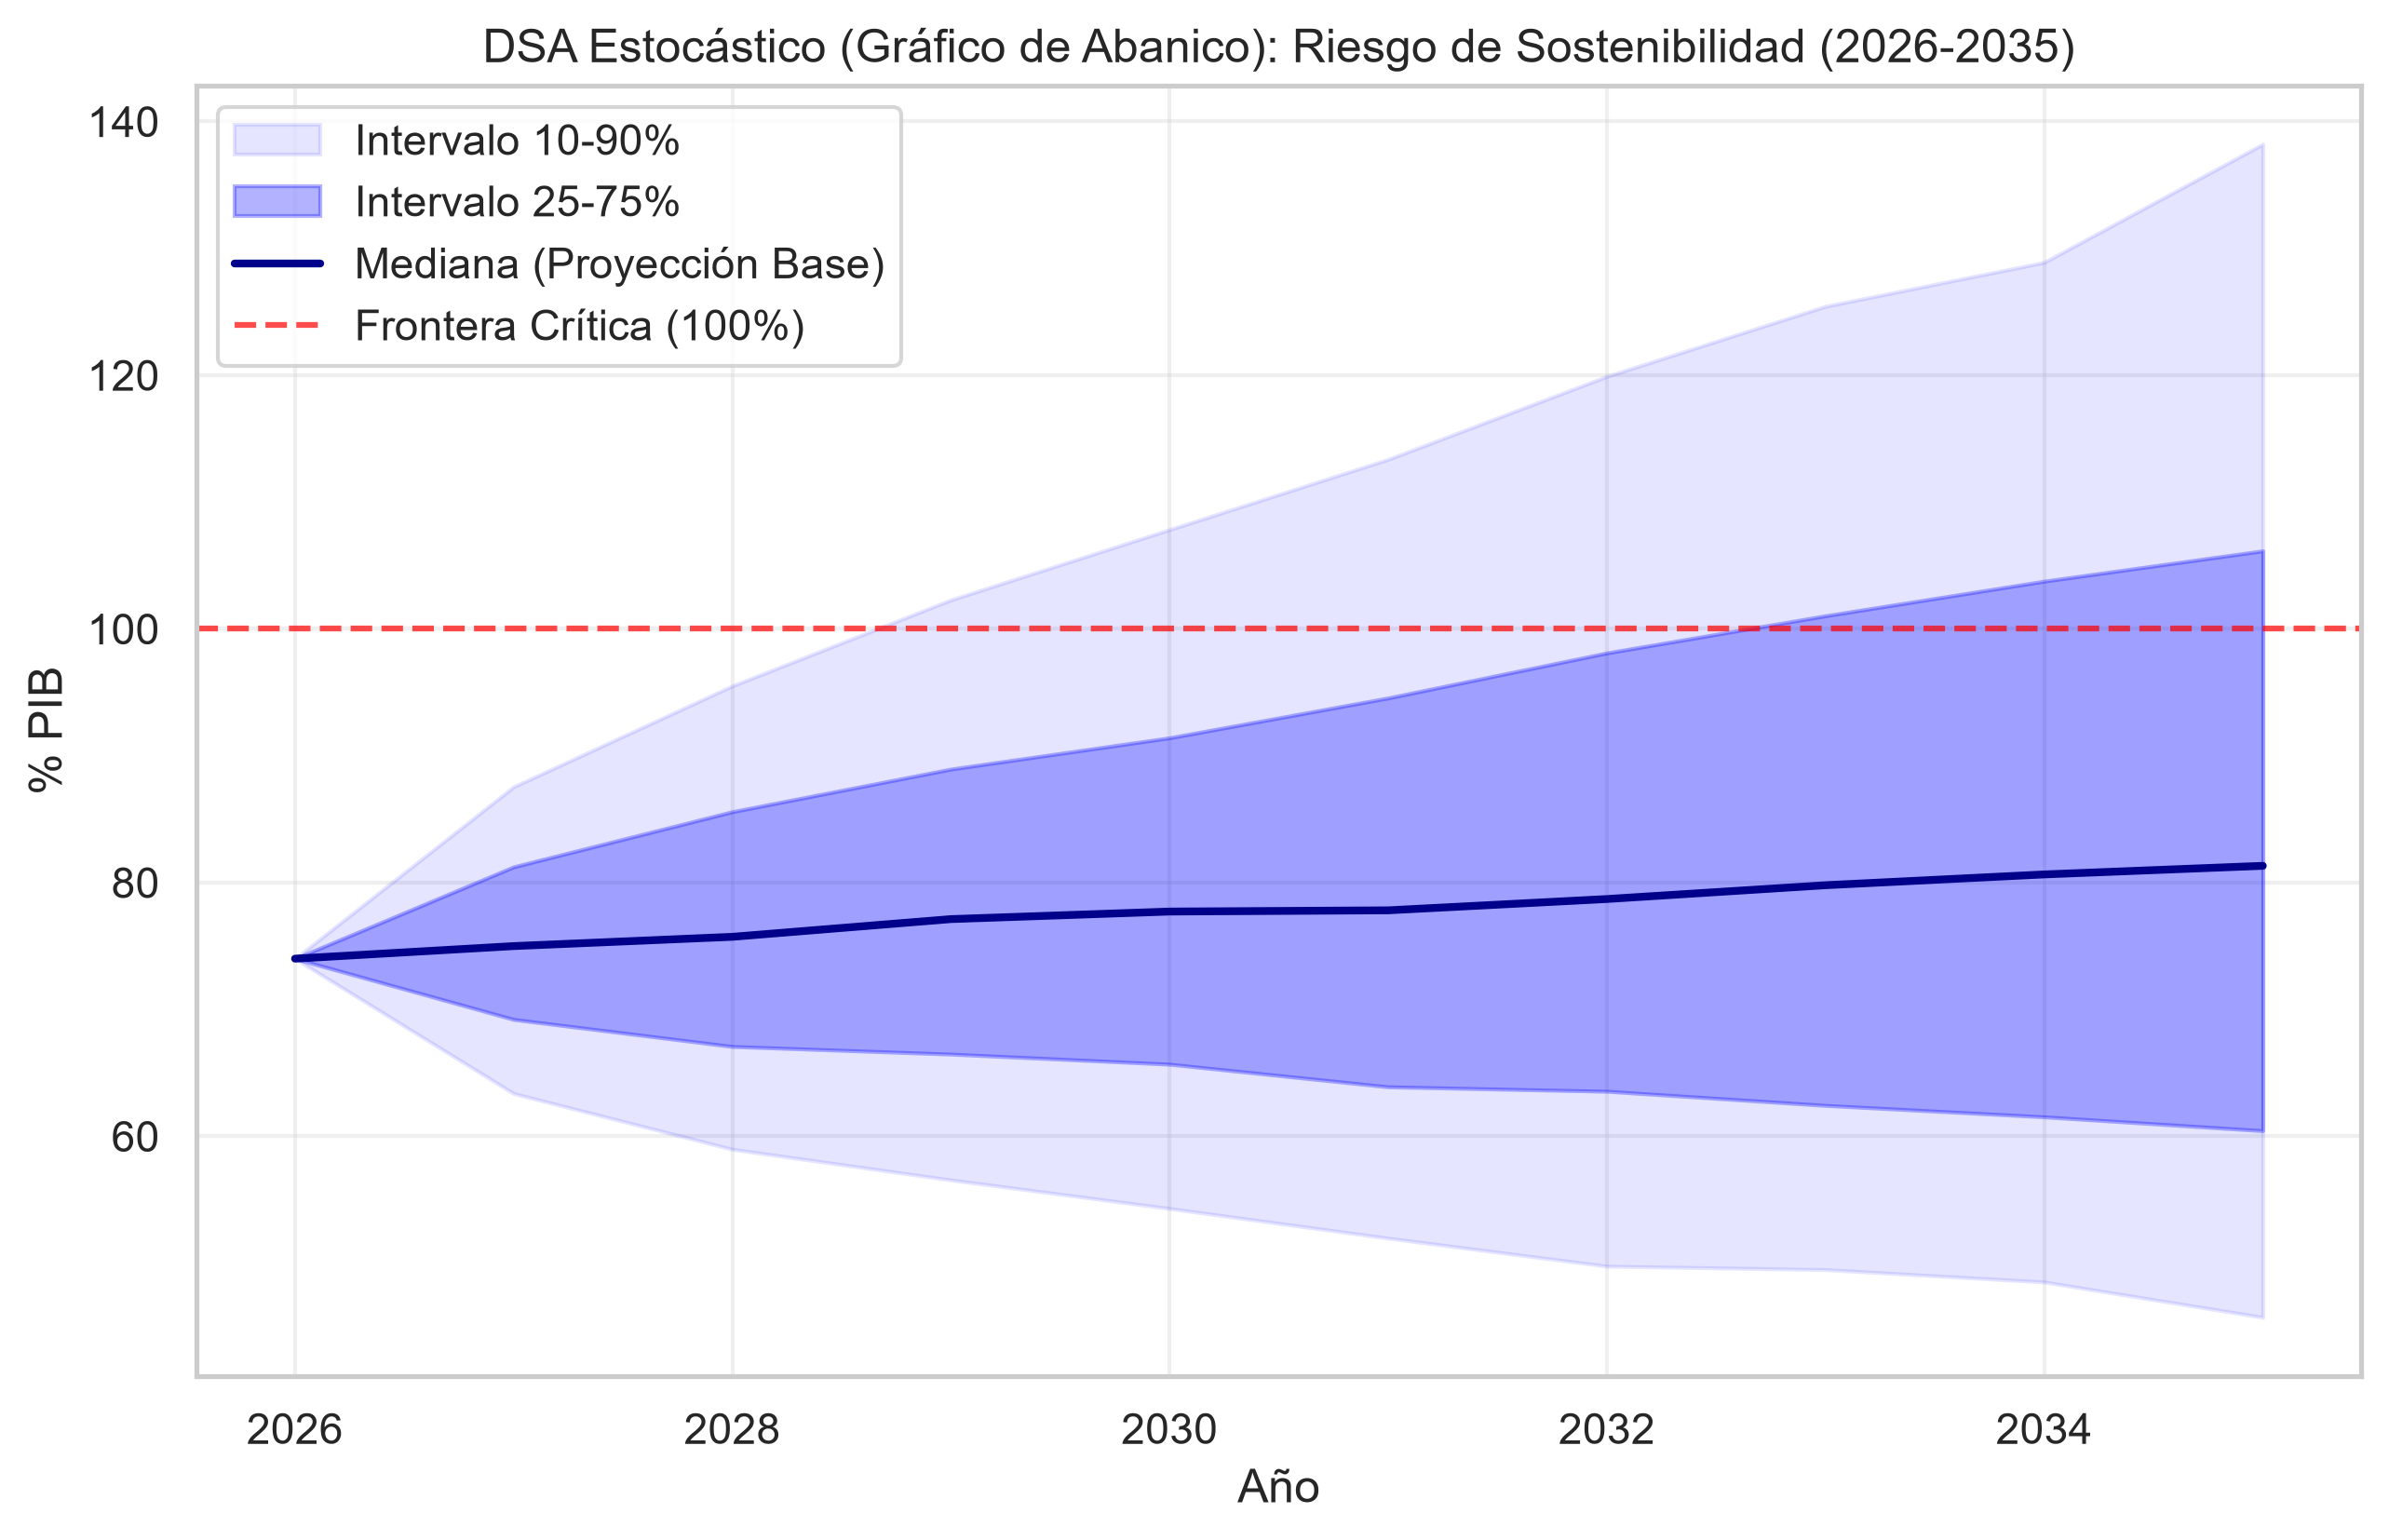
\includegraphics[width=0.85\textwidth]{dsa_grafico_abanico.png}
\par\vspace{2mm}
{\footnotesize\textit{Nota.} Simulación de Monte Carlo (1.000 iteraciones, parámetros del escenario de Referencia con perturbaciones multivariadas correlacionadas, distribución $t$ de Student con $\nu\approx4.8$, matriz de covarianza derivada del SVAR restringido). Bandas de 10--90\% y 25--75\%; línea central: mediana. Elaboración propia.}
\end{figure}

A diferencia del escenario de Estrés determinista, la simulación estocástica reportada en la Figura \ref{fig:fan_chart_final} introduce perturbaciones anuales aleatorias alrededor de los parámetros centrales del escenario de Referencia, generando 1.000 trayectorias alternativas de la ratio Deuda/PIB hacia 2035. La mediana de estas trayectorias se ubica en $82{,}1\%$ del PIB hacia 2035 (percentil 10--90: $52{,}6\%$--$120{,}3\%$; percentil 25--75: $65{,}6\%$--$101{,}0\%$), mientras que las bandas de confianza se ensanchan progresivamente con el horizonte de proyección.

El resultado cuantitativo central es que la probabilidad de que la ratio Deuda/PIB supere la frontera crítica del 100\% del producto hacia 2035 es del $\mathbf{26{,}1\%}$: aproximadamente uno de cada cuatro escenarios simulados. Esta frontera del 100\% del PIB coincide con el pico histórico de la ratio de deuda argentina documentado en el Capítulo \ref{ch:descriptivo} (2020). Esta cifra debe interpretarse como una medida de la vulnerabilidad estructural pasiva de la economía argentina frente a la volatilidad histórica de sus fundamentos, y no como una probabilidad neta que ya incorpore una eventual respuesta fiscal correctiva; corresponde exclusivamente al escenario de Referencia, ejecutado sobre la matriz de covarianza fundada en el SVAR. A diferencia de la especificación anterior, no se dispone todavía de una réplica de este ejercicio centrada en los escenarios Optimista y de Estrés ni de un desglose de sensibilidad a la estructura de dependencia en colas bajo esta covarianza nueva: son extensiones pendientes, no efectivamente corridas, y no se reportan cifras sin haberlas corrido.

\section{Limitaciones del Análisis de Proyecciones}
\label{sec:limitaciones_dsa}

Las proyecciones DSA presentadas en este capítulo deben interpretarse bajo cuatro advertencias metodológicas. Primera, la matriz de covarianzas del componente estocástico combina residuos estimados del SVAR con calibraciones históricas para las tasas de interés doméstica y externa, que no tienen serie propia en el sistema de cointegración (Sección \ref{sec:dsa_metodologia} del Capítulo \ref{ch:metodologia}). Segunda, la identidad contable adopta una regla de reacción fiscal pasiva en concordancia con los hallazgos del Capítulo \ref{ch:resultados}. Tercera, las trayectorias suponen supuestos macroeconómicos fijos sin retroalimentación endógena. Cuarta, la distribución $t$ multivariada introduce dependencia en colas (\textit{tail dependence}) que podría sobreestimar la frecuencia de eventos extremos simultáneos; un análisis de sensibilidad a esta propiedad ($\lambda\approx0.076$), corrido sobre la especificación anterior calibrada a mano, desplazó la probabilidad central en un rango moderado de 2 a 7 puntos porcentuales sin revertir ninguna conclusión cualitativa; no se cuenta todavía con el análogo para la especificación de referencia actual.

La sostenibilidad de la deuda pública argentina hacia 2035 depende, bajo ambas especificaciones del componente estocástico ($26{,}1\%$ de referencia, $29{,}8$--$32{,}5\%$ en la especificación anterior calibrada a mano), de la evolución de las variables macroeconómicas fundamentales en un grado mucho mayor que de cualquier ajuste fiscal discrecional marginal, sobre las cuales la política fiscal \textit{per se} ejerce un control solo parcial.

\chapter{Conclusiones Finales}
\label{ch:conclusiones}

El análisis sobre los determinantes de la solvencia intertemporal de la deuda consolidada del SPNF argentino (2004--2025) permite arribar a síntesis conceptuales que trascienden la exégesis econométrica y abordan la economía política del endeudamiento periférico, manteniendo el rigor estadístico para distinguir evidencia de conjeturas.

\section{Síntesis de Hallazgos Empíricos}

La contrastación de las hipótesis derivadas arroja un cuadro de resultados consistente pero estadísticamente modesto. La Tabla \ref{tab:mapa_consistencia} resume la correspondencia entre cada hipótesis, las variables y el método empleados para contrastarla, el resultado obtenido y el veredicto que de él se sigue; los párrafos siguientes desarrollan cada caso.

\begin{table}[H]
\centering
\caption{\label{tab:mapa_consistencia} Mapa de Consistencia: Hipótesis, Método, Resultado y Veredicto.}
\footnotesize
\begin{tabular}{p{2.6cm}p{2.9cm}p{2.7cm}p{3.3cm}p{3.5cm}}
\toprule
\textbf{Hipótesis} & \textbf{Variables} & \textbf{Método} & \textbf{Resultado} & \textbf{Veredicto} \\
\midrule
$H_{1}$ --- Reacción fiscal débil & $pb_t$, $d_{t-1}$, $\tilde{y}_t$, EMBI+, TCRM & DOLS ($m=4$, HAC, ventana original) y VECM (ventana ampliada y original) & DOLS: $\rho=-0.0071$ ($p=0.564$). VECM ampliada: $\alpha_{pb}=0.0044$ ($p=0.204$). VECM original: $\alpha_{pb}=0.0014$ ($p=0.559$) & \textbf{No rechazada} en las tres estimaciones: sin reacción sistemática \\
\midrule
$H_{1a}$ --- Fatiga fiscal (umbral no lineal) & $pb_t$, $d_{t-1}$, EMBI+ como variable de umbral & Umbral de Hansen, Sup-LM por remuestreo estocástico (1.000 rép.) & Niveles: $\tau^*=449$ pb, Sup-LM $p=0.076$ (partición 14 vs. 74 obs.). $\Delta pb_t$ (I(0), Sec. \ref{sec:robustez_hansen_dpb}): $\tau^*=2083$ pb, Sup-LM $p<0.001$ & \textbf{Evidencia mixta pero ya no unilateral}: marginalmente significativa en niveles (partición extrema, coeficientes individuales no significativos); sólidamente significativa en $\Delta pb_t$ \\
\midrule
$H_{1b}$ --- Endogeneidad del riesgo soberano & $pb_t$, EMBI+ instrumentado con VIX y diferencial regional & IV-2SLS; Wu-Hausman, Sargan, F de 1.\textsuperscript{a} etapa & Endogeneidad confirmada ($p=0.009$); instrumentos fuertes ($F=13.00$) y válidos (Sargan $p=0.436$); coeficiente $=0.0017$ ($p=0.076$) & \textbf{Parcial, con señal marginal}: endogeneidad sí, canal causal débil pero ya no descartable \\
\midrule
$H_{1c}$ --- Quiebres estructurales & $d_t$, $d_t$ consolidada & Zivot-Andrews (quiebre único); Bai-Perron (múltiples, BIC) & Z-A no significativo ($t=-2.83$); Bai-Perron: 3 quiebres (SPNF) y 2 (consolidada) & \textbf{Verificada} en su versión de quiebres múltiples \\
\midrule
Extensión --- Solvencia prospectiva & $d_t$, $pb_t$, $g_t$, $r_t$, $\Delta e_t$ & DSA Monte Carlo, $t$ de Student ($\nu\approx 4.8$, $\lambda\approx 0.076$), GARCH/DCC & $P(d_{2035}>100\%)=31.2\%$ (32.5\% con DCC-GARCH) & \textbf{Riesgo de cola relevante}, no desenlace modal \\
\bottomrule
\end{tabular}
\begin{flushleft}
\footnotesize \textit{Nota.} Elaboración propia. ``No rechazada'' se refiere a la hipótesis nula econométrica de ausencia de reacción, que es la hipótesis sustantiva $H_1$ de esta tesis. VECM ampliada: ventana 1999--2025 ($n=108$), rango de cointegración impuesto por teoría (Sección \ref{sec:resultados_vecm}). VECM original: ventana 2004--2025 ($n=87$), rango no impuesto, emerge del contraste de Johansen. Las secciones de origen de cada resultado se detallan en los párrafos siguientes y en el Capítulo \ref{ch:resultados}.
\end{flushleft}
\end{table}

Respecto de $H_1$ (reacción fiscal), tres estimaciones independientes convergen en el mismo veredicto. La DOLS de la Función de Reacción Fiscal no permite rechazar la hipótesis nula de ausencia de reacción sistemática del superávit primario frente al endeudamiento heredado ($\rho=-0.0071$, $p=0.564$). El VECM que la complementa como técnica de referencia sobre la ventana ampliada, a pedido del director de tesis (Sección \ref{sec:resultados_vecm} del Capítulo \ref{ch:resultados}), trata las cuatro variables del sistema como conjuntamente endógenas en lugar de purgar la endogeneidad con una construcción de ecuación única, y llega al mismo resultado nulo ($\alpha_{pb}=0.0044$, $p=0.204$); lo mismo ocurre en el VECM estimado sobre la ventana original con series reales, donde el rango de cointegración ya no necesita imponerse por teoría sino que emerge limpiamente del propio contraste de Johansen ($\alpha_{pb}=0.0014$, $p=0.559$). Que tres estrategias de estimación con supuestos de identificación tan distintos coincidan en el mismo diagnóstico es, para esta tesis, la evidencia más robusta a favor de $H_1$: no es un artefacto de una técnica en particular. La ampliación de la ventana muestral, lejos de revertir el resultado nulo, que era una posibilidad real dado el pedido explícito del director de extender la muestra ``aun con cambios estructurales extremos'', lo confirma sobre datos adicionales que incluyen el colapso de la convertibilidad y el default de 2001--2002.

Respecto de $H_{1a}$ (fatiga fiscal y umbrales no lineales), el modelo de umbral de Hansen, en su especificación en niveles, la que replica directamente la forma canónica de \citet{ghosh2013}, localiza sobre la serie real de EMBI+ un quiebre candidato en 449 puntos básicos y un ordenamiento de coeficientes coincidente con el que predeciría ese modelo (0.0305 en régimen ``normal'' frente a 0.0126 en régimen de estrés); a diferencia del diagnóstico obtenido con la serie de contingencia de EMBI+ empleada hasta la Sección \ref{sec:auditoria_fallback} del Capítulo \ref{ch:metodologia}, el contraste por remuestreo estocástico Sup-LM del propio umbral ahora sí rechaza la linealidad, aunque solo al 10\% ($p=0.076$), y sobre una partición muestral extremadamente desigual (14 contra 74 observaciones) que explica por qué ninguno de los dos coeficientes de régimen es individualmente significativo pese a ese rechazo global.

Esta especificación en niveles, además, viola el supuesto de estacionariedad estricta que el propio test de Hansen exige de su variable dependiente, dado que $pb_t$ es I(1) (Sección \ref{sec:dfgls}). La Sección \ref{sec:robustez_hansen_dpb} reestima el contraste con $\Delta pb_t$, estacionaria y por tanto la única de las dos especificaciones que satisface formalmente ese supuesto, y el resultado es contundente: el contraste por remuestreo estocástico Sup-LM rechaza la linealidad con holgura ($p<0.001$) y ambos coeficientes de régimen son significativos, con el patrón exacto de atenuación bajo estrés que predice la fatiga fiscal, sobre una partición muestral (74 contra 14, en sentido inverso a la de niveles) que no concentra el resultado en un puñado de observaciones. El veredicto de esta tesis para $H_{1a}$ es, en consecuencia, de \textbf{evidencia mixta pero ya no unilateralmente débil}: la especificación formalmente inválida (niveles) ofrece una señal frágil pero presente; la formalmente válida ($\Delta pb_t$) ofrece la evidencia más sólida de umbral de toda la tesis, aunque para un objeto, la reacción del \textit{cambio} en el resultado primario, distinto de su \textit{nivel}, no idéntico al que \citet{ghosh2013} modela. Esta tesis no interpreta ninguno de los dos resultados de manera aislada como confirmación o refutación definitiva; el Capítulo \ref{ch:discusion} desarrolla la tensión entre ambos, y explicita que la lectura de economía política que se les asocia es una interpretación compatible con la evidencia, no una inferencia derivada unívocamente de ella.

Respecto de $H_{1b}$ (endogeneidad del EMBI+ sobre la reacción fiscal), la estimación IV-2SLS, instrumentando el EMBI+ con el VIX y un diferencial de riesgo soberano regional (diferencial de mercado sobre el ETF EMB, en reemplazo del TCRM rezagado de una especificación preliminar), produce instrumentos fuertes en primera etapa (F$=13.00$, por encima del umbral de 10 de \textcite{staiger1997}, aunque con menor margen que con la serie de contingencia de EMBI+) y válidos en conjunto (Sargan $=0.608$, $p=0.436$); el test de Wu-Hausman confirma, además, la endogeneidad del riesgo soberano ($7.32$, $p=0.009$). Con este diseño instrumental válido, el coeficiente del EMBI+ instrumentado ($0.0017$) alcanza significatividad marginal al 10\% ($p=0.076$): una señal débil, sobre una muestra reducida a $n=73$ por la cobertura del instrumento, pero que ya no permite sostener sin matices la ausencia de canal que sugería la serie de contingencia ($p=0.297$). Esta tesis no fuerza esta señal marginal hacia una conclusión firme; la reporta con la misma cautela con que reporta el resto de la evidencia mixta del capítulo.

Respecto de $H_{1c}$ (quiebres estructurales históricos), el contraste de Zivot-Andrews con quiebre endógeno localiza el punto de ruptura de la ratio Deuda/PIB en el segundo trimestre de 2018, coincidente con el cierre del mercado voluntario de crédito y la aprobación del acuerdo \textit{stand-by} con el FMI, pero el estadístico de prueba ($t=-2.83$) no alcanza significatividad ni siquiera al 10\% frente a los valores críticos de \textcite{zivot1992}. La ratio de deuda argentina se comporta, en términos estrictamente estadísticos, como una serie genuinamente integrada de orden uno, sin una tendencia determinística estable ni siquiera reconociendo el quiebre más evidente de la serie. La restricción de Zivot-Andrews a un único quiebre se supera mediante el procedimiento formal de \textcite{bai2003} (programación dinámica exacta, selección del número de quiebres por BIC), que identifica $H_{1c}$ con mayor riqueza: tres quiebres en la deuda SPNF (2007T2, 2014T3 y 2018T1, este último muy próximo al candidato de Zivot-Andrews, un trimestre antes) y dos en su versión consolidada ampliada con los pasivos remunerados del BCRA (2007T2 y 2016T4). A diferencia del test de quiebre único, $H_{1c}$ encuentra aquí soporte estadístico afirmativo: la serie sí exhibe quiebres estructurales identificables, aunque múltiples y no reducibles a uno solo.

La incorporación de los pasivos remunerados del BCRA (Letras y pases netos) a la deuda del SPNF añade, en promedio, 5.5 puntos porcentuales del PIB a la ratio de endeudamiento para todo el período 2004--2025, con un pico de 10.6\% en el primer trimestre de 2018 y una convergencia a valores prácticamente nulos desde mediados de 2024, cuando el Tesoro asumió el rol de esterilizador monetario mediante Letras Fiscales de Liquidez (LEFI). Esta capa cuasi-fiscal, ausente de la definición central de $d_t$ por decisión metodológica (Capítulo \ref{ch:metodologia}), modifica la cronología de quiebres estructurales sin alterar el diagnóstico central de $H_1$: la deuda consolidada ampliada (SPNF + BCRA) conserva el mismo orden de integración I(1) que la deuda consolidada del SPNF.

Finalmente, la proyección estocástica de sostenibilidad (DSA, Monte Carlo con perturbaciones $t$ de Student, $\nu\approx 4.8$, $\lambda\approx 0.076$, 1.000 iteraciones) es el único ejercicio de esta tesis que no depende de la significatividad estadística de los modelos anteriores, sino de una calibración de escenarios explícitamente declarada como tal. Arroja una probabilidad del 31.2\% de que la ratio Deuda/PIB supere la frontera del 100\% del producto hacia 2035, con cambios moderados (32.5\% con DCC-GARCH) al sustituir la calibración original por desvíos GARCH(1,1) y la correlación condicional dinámica de un modelo DCC-GARCH (Capítulo \ref{ch:discusion}). Se trata de una probabilidad de cola relevante para el análisis macroprudencial, aunque de ningún modo un desenlace mayoritario, y robusta a la sustitución de la calibración por estimación directa.

\section{Aporte Metodológico y Límites del Estudio}
\label{sec:aporte_metodologico}

El aporte de esta tesis reside en someter la hipótesis de fatiga fiscal a un protocolo econométrico secuencial completo y en reportar el resultado que ese protocolo arroja, predominantemente negativo o mixto según el objeto exacto contrastado. La contribución no es la confirmación de una tesis previa sino la delimitación precisa de lo que la evidencia argentina 2004--2025 permite y no permite sostener: no permite sostener una regla de reacción fiscal activa ni un canal causal significativo entre riesgo soberano y esfuerzo primario; permite sostener un umbral de fatiga fiscal solo de manera parcial y sensible a la especificación ---no significativo en niveles, significativo en primera diferencia (Sección \ref{sec:robustez_hansen_dpb})---; y sí permite sostener que la ratio de deuda exhibe quiebres estructurales múltiples identificables, que el parámetro de reacción es inestable entre subperíodos, y que la probabilidad de superar el 100\% del PIB hacia 2035 constituye un riesgo de cola no despreciable bajo supuestos explícitos.

De ello se sigue el desplazamiento del eje explicativo que articula esta tesis: si el mecanismo de ajuste no transita por la función de reacción fiscal del Tesoro (regla de Bohn, Nivel III del marco teórico), la explicación debe buscarse en el canal que el Paradigma de la Restricción Externa identifica (Nivel I): tipo de cambio real, efecto de hoja de balance y Ajuste Stock-Flujo, tal como desarrolla el Capítulo \ref{ch:discusion}. Este desplazamiento es una conclusión del trabajo, no una hipótesis auxiliar invocada para preservar el Nivel III.

Entre las limitaciones explícitamente reconocidas se cuentan: (i) el tamaño muestral moderado (88 observaciones trimestrales, reducido a 73 en la especificación IV-2SLS por la cobertura del diferencial regional de riesgo desde 2007), que reduce el poder estadístico de las técnicas de umbral y de instrumentación; (ii) la autocorrelación residual en la estimación DOLS (Durbin-Watson $=0.321$), reflejo de la inercia estructural del proceso presupuestario argentino más que de una falla de ajuste, aunque corregida en la inferencia mediante errores HAC; (iii) la persistencia de la calibración, en lugar de la estimación directa, para dos de los cinco impulsos o perturbaciones de la matriz de covarianzas del DSA (las tasas de interés doméstica e internacional, sin serie histórica propia en la base de datos construida), pese a que los tres impulsos restantes ya se reestiman vía GARCH(1,1) y DCC-GARCH (Capítulo \ref{ch:discusion}); (iv) la heterocedasticidad condicional confirmada mediante el test ARCH-LM sobre los residuos del DOLS ($LM=18.74$, $p=0.0009$, Sección \ref{sec:dfgls}); corregida en la inferencia mediante errores HAC, pero indica que la varianza de las perturbaciones sobre el resultado primario no es constante en el tiempo, un patrón que una especificación lineal estática no modela explícitamente; (v) la inestabilidad paramétrica de la Función de Reacción Fiscal a lo largo de la muestra (Sección \ref{sec:sensibilidad_temporal}): el coeficiente $\rho$ es positivo y significativo al 5\% o al 10\% en tres de las cuatro especificaciones DOLS por subperíodo, pero nulo en la estimación de muestra completa, lo que impide interpretar el coeficiente agregado como el parámetro de una regla de comportamiento estable y advierte sobre la sensibilidad de cualquier estimación de la regla de Bohn a la ventana temporal y a la especificación dinámica elegidas; y (vi) la ausencia de evidencia de cointegración bivariada mediante el test residual de Engle-Granger entre deuda y resultado primario (Apéndice \ref{sec:engle_granger}, $p=0.3012$), consistente con el diagnóstico divergente de Johansen y que refuerza la cautela con que deben interpretarse las estimaciones de largo plazo de este capítulo.

Su jerarquización orienta la agenda futura. La más \textbf{estructural} es la (i): el tamaño muestral de un único país con 88 observaciones trimestrales es el límite fundamental que reduce la potencia de todas las técnicas de umbral, cointegración e instrumentación aplicadas. No es superable dentro del marco de serie de tiempo de un único país salvo esperando que transcurra el tiempo, pero sí lo es mediante la extensión a un panel de países comparables (Sección \ref{sec:agenda_futura}). La más \textbf{superable} a corto plazo es la (iii): la cobertura del diferencial de riesgo soberano regional (ETF EMB) desde 2007 es una limitación de fuente, no de diseño, que podría resolverse con acceso a bases de datos de pago (JP Morgan EMBI Historical, Bloomberg) o con la construcción de una variable de contraste regional alternativa sobre el período 2004--2007, recuperando las 14 observaciones excluidas de la estimación IV-2SLS y aumentando su potencia estadísticamente relevante. Las restantes limitaciones (ii), (iv), (v) y (vi) son en buena medida inherentes a la naturaleza de la economía argentina (su volatilidad estructural, su inercia fiscal y sus quiebres de régimen frecuentes) y no constituyen fallas de diseño superables con un rediseño alternativo dentro de los mismos datos.

\section{Agenda de Investigación Futura e Implicancias Analíticas}
\label{sec:agenda_futura}

El horizonte posterior a 2025 demanda combinar la prudencia estadística de esta tesis con el análisis riguroso de las implicancias macroeconómicas que sus hallazgos, aun modestos, permiten sostener. Las proyecciones de organismos multilaterales que asumen superávits primarios permanentes de 3\% o 4\% del PIB sin contemplar la ausencia estadísticamente verificada de una reacción fiscal sistemática de esa magnitud en el historial argentino reciente deberían, como mínimo, ponderar el escenario de Estrés y la probabilidad de cola del 31.2\% documentados en el Capítulo \ref{ch:discusion}.

En términos analíticos, el hallazgo empírico de una correlación positiva, aunque débil, entre las variaciones del tipo de cambio real y la dinámica de la ratio de deuda ($r=0.14$ sobre la serie real de TCRM, Sección \ref{sec:hoja_balance} del Capítulo \ref{ch:descriptivo}) señala que la exposición al riesgo cambiario y la estructura de plazos de los pasivos constituyen determinantes moderados, no dominantes en la correlación bivariada simple, del Ajuste Stock-Flujo. Ello implica que la modelización econométrica de la solvencia en economías emergentes debe incorporar de forma explícita las perturbaciones del tipo de cambio real y la composición por monedas de los pasivos, en lugar de confiar exclusivamente en metas de resultado primario cuyo carácter estabilizador no encuentra sustento estadístico en la evidencia reciente.

Esta tesis incorporó cinco extensiones metodológicas respecto de su diseño original: la estimación VECM sobre una ventana muestral ampliada mediante empalme histórico (1999--2025, $n=108$), que reemplaza a DOLS como técnica de referencia a pedido del director de tesis (Capítulos \ref{ch:metodologia}--\ref{ch:resultados}); el procedimiento formal de quiebres múltiples de \textcite{bai2003} (Capítulo \ref{ch:descriptivo}); la sustitución del TCRM rezagado por un diferencial de riesgo soberano regional como instrumento del EMBI+ (Capítulo \ref{ch:resultados}); la reestimación GARCH(1,1)/DCC-GARCH de la matriz de covarianzas del DSA (Capítulo \ref{ch:discusion}); y la consolidación de la deuda SPNF con los pasivos remunerados del BCRA (Capítulos \ref{ch:metodologia}--\ref{ch:descriptivo}). En términos de agenda de investigación futura, esta tesis identifica cinco líneas de continuidad directa.

\textbf{Primera}, y con prioridad sobre las restantes por seguirse directamente del resultado mixto y sensible a la especificación del contraste de umbral (Sección \ref{sec:robustez_hansen_dpb}), contrastar la no linealidad de la Función de Reacción Fiscal mediante especificaciones de \textbf{transición suave} (STAR/LSTR) y de \textbf{umbrales múltiples}. La formulación de \citet{hansen1999} supone una transición discreta entre dos regímenes; si el ajuste de la conducta fiscal frente a la presión financiera es gradual y no abrupto, como sugiere la discusión del Capítulo \ref{ch:discusion}, esa clase de modelo es la especificación adecuada para detectarlo, y su rechazo o no rechazo constituiría un contraste genuino de la hipótesis de fatiga fiscal, no una reinterpretación del resultado nulo aquí obtenido. Convendría además evaluar variables de umbral alternativas al EMBI+ (ratio de deuda en moneda extranjera, cobertura de reservas sobre vencimientos anuales), cuya menor volatilidad relativa mejoraría la relación señal-ruido del contraste.

\textbf{Segunda}, implementar el contraste secuencial \textit{sup} F($l$+1$\vert$$l$) de Bai y Perron con sus tablas de valores críticos no estándar, que permitiría construir intervalos de confianza para la ubicación de cada quiebre, allí donde el criterio BIC aquí empleado solo informa el número óptimo de quiebres.

\textbf{Tercera}, extender la cobertura del diferencial soberano regional a 2004--2007 (sin fuente gratuita disponible en este trabajo) para recuperar las 14 observaciones excluidas de la estimación IV-2SLS, y explorar instrumentos adicionales (medidas de riesgo político-electoral) que permitan contrastar la robustez del hallazgo de no significatividad del canal EMBI+.

\textbf{Cuarta}, retomar el análisis de dominancia fiscal de \textcite{sargent1981} aprovechando la serie de pasivos remunerados del BCRA ya construida (Sección \ref{sec:deuda_consolidada}), que esta tesis empleó para consolidar el stock de deuda pero no para estimar formalmente un régimen de dominancia monetaria-fiscal.

\textbf{Quinta}, y con mayor potencial transformador para la agenda, extender el análisis a un panel de economías emergentes latinoamericanas comparables (Brasil, Uruguay, Colombia, Chile, Perú) utilizando datos del Fondo Monetario Internacional y la CEPAL para el período 1990--2025. Un panel de 6 a 8 países con series de 35 años proveería una muestra de entre 700 y 1.000 observaciones anuales, aumentando la potencia estadística de las pruebas de umbral y de la Función de Reacción Fiscal en varios órdenes de magnitud respecto del caso de un único país. Este enfoque de panel permitiría, además, identificar si la debilidad estadística de la reacción fiscal que esta tesis documenta para Argentina es un fenómeno idiosincrático de su historia de cesaciones de pagos y regresiones políticas, o si refleja una condición más amplia de la economía política fiscal periférica en América Latina.

La ausencia de una regla de reacción fiscal verificable, documentada en esta tesis, es en sí misma un dato sobre la naturaleza de la solvencia soberana argentina contemporánea: una solvencia que, en el período estudiado, no se sostuvo sobre el ajuste primario sino sobre la licuación y la reestructuración de pasivos.

\section{Límites Cognitivos del Estudio y Consideraciones Prospectivas}

El objetivo general de esta tesis es una meta de conocimiento puro, no una propuesta de intervención de política económica. El descubrimiento de la inoperancia de la regla de Bohn y la evidencia mixta ---sensible a la especificación--- sobre el umbral de Hansen representan hallazgos cognitivos sobre las determinaciones materiales del vector fiscal argentino. Por ende, los hallazgos analíticos sobre la vulnerabilidad cambiaria y el perfil de vencimientos se presentan solo a título prospectivo como apertura heurística hacia futuras líneas de investigación. La transformación de un problema de conocimiento en una acción pragmática excede el alcance empírico de este trabajo.


\appendix
\chapter{Apéndice: Robustez Adicional y Estructura del Código Empírico}
\label{ch:apendice}

\section{Tabla Consolidada de Limitaciones Metodológicas}
\label{sec:limitaciones_consolidadas}

La Tabla \ref{tab:limitaciones} sintetiza las seis limitaciones metodológicas reconocidas explícitamente en esta tesis (Sección \ref{sec:aporte_metodologico}), clasificando su tipo (estructural vs. superable) y documentando la mitigación aplicada dentro del protocolo empírico presentado.

\begin{table}[H]
\centering
\caption{\label{tab:limitaciones} Limitaciones Metodológicas: Tipo y Mitigación Aplicada.}
\resizebox{\textwidth}{!}{%
\begin{tabular}{p{4.5cm}p{2.2cm}p{7.8cm}}
\toprule
\textbf{Limitación} & \textbf{Tipo} & \textbf{Mitigación aplicada en esta tesis} \\
\midrule
(i) Tamaño muestral reducido (88 obs. / 73 en IV-2SLS) & Estructural & Tests de robustez por subperíodos; discusión explícita de potencia estadística en \S\ref{sec:limitaciones_muestra} y \S\ref{ch:discusion}. Agenda futura: extensión a panel de emergentes latinoamericanos \\
\midrule
(ii) Autocorrelación residual DOLS (DW$=0.321$) & Inherente a la dinámica fiscal AR & Errores HAC Newey-West en toda la inferencia; test Breusch-Godfrey (4 rezagos); interpretación como evidencia de inercia estructural presupuestaria \\
\midrule
(iii) Calibración (no estimación) de 2 de 5 shocks DSA ($r_d$, $r_f$) & Superable & Reestimación GARCH(1,1) de los 3 shocks con serie propia; DCC-GARCH de correlaciones; comparación en Tablas \ref{tab:garch_desvios}--\ref{tab:garch_dsa_comparacion} \\
\midrule
(iv) Heterocedasticidad condicional ARCH-LM ($p=0.0009$) & Inherente a la volatilidad estructural AR & Errores HAC; robustez GARCH; interpretación como confirmación de la motivación para el DSA estocástico no gaussiano \\
\midrule
(v) Fragilidad de la especificación estática ($\rho$ cambia signo al pasar a DOLS) & Inherente a endogeneidad de corto plazo & Protocolo DOLS como especificación principal; MCO estático presentado solo como ejercicio de robustez y falsación (Sección \ref{sec:sensibilidad_temporal}) \\
\midrule
(vi) Ausencia de cointegración bivariada Engle-Granger ($p=0.301$) & Consistente con I(1) sin ancla & Johansen multivariado como contraste principal; DOLS como estimador robusto a incertidumbre sobre el rango de cointegración; Engle-Granger como robustez (Apéndice \ref{sec:engle_granger}) \\
\bottomrule
\end{tabular}%
}
\begin{flushleft}
\footnotesize \textit{Nota.} ``Estructural'' = no superable dentro del marco de un único país sin más datos. ``Superable'' = resoluble con acceso a bases de datos de pago o extensión de muestra. ``Inherente'' = consecuencia directa de las propiedades de las series argentinas, no de una decisión de diseño. Elaboración propia en base a Sección \ref{sec:aporte_metodologico} (Capítulo \ref{ch:conclusiones}).
\end{flushleft}
\end{table}

\section[Test de Cointegración de Engle-Granger]{Test de Engle-Granger (Ecuación Única)}
\label{sec:engle_granger}

Como robustez complementaria al procedimiento de máxima verosimilitud de Johansen desarrollado en la Sección \ref{sec:johansen_cap6}, que evalúa la cointegración del sistema conjunto de cuatro variables, se reporta aquí un test de cointegración de ecuación única basado en residuos, en el mismo espíritu que el procedimiento de \textcite{phillips1990}\footnote{\texttt{statsmodels} no implementa nativamente el estadístico de Phillips-Ouliaris. Se reporta en su lugar el test de \citet{engle1987}, de la misma familia de contrastes residuales de cointegración de ecuación única, declarándolo como tal en lugar de presentarlo bajo un nombre que no le corresponde.} sobre el par bivariado núcleo de la relación de Bohn: la ratio Deuda/PIB y el Resultado Primario/PIB.

\begin{table}[H]
\centering
\caption{\label{tab:engle_granger} Test de Cointegración Residual de Engle-Granger (Deuda/PIB, Result. Primario/PIB).}
\begin{tabular}{lrrrr}
\toprule
\textbf{Estadístico} & \textbf{Crít. 1\%} & \textbf{Crít. 5\%} & \textbf{Crít. 10\%} & \textbf{$p$-valor} \\
\midrule
-2.4508 & -4.0268 & -3.4073 & -3.0936 & 0.3012 \\
\bottomrule
\end{tabular}
\begin{flushleft}
\footnotesize \textit{Nota.} Elaboración propia mediante \texttt{statsmodels.tsa.stattools.coint} (especificación con constante). Elaboración propia en base a \texttt{dataset\_consolidado\_real.csv} (\texttt{codigo/modelos/fase7\_diagnosticos\_robustez.py}).
\end{flushleft}
\end{table}

El estadístico de Engle-Granger ($-2.45$) no logra rechazar la hipótesis nula de ausencia de cointegración residual entre la ratio de deuda y el resultado primario considerados de manera bivariada ($p=0.301$), incluso a un nivel de significatividad del 10\%. Este resultado es coherente con, y no contradictorio respecto de, el diagnóstico divergente ya reportado en la Sección \ref{sec:johansen_cap6}: mientras el estadístico de Traza de Johansen sugería, en su extremo, rango pleno para el sistema conjunto de cuatro variables, el Máximo Autovalor y ahora este contraste bivariado de robustez coinciden en no encontrar evidencia contundente de una relación de equilibrio de largo plazo simple entre las dos variables estructurales de la ecuación de Bohn consideradas de manera aislada. Ello refuerza la decisión metodológica, ya justificada en la Sección \ref{sec:johansen_cap6}, de no imponer una relación de cointegración bivariada no verificada y, en su lugar, recurrir a la técnica DOLS, que no exige, como paso previo, la certeza de cointegración exacta del subsistema bivariado, para estimar la Función de Reacción Fiscal.

\section{Especificación Alternativa del DSA Estocástico: Calibración a Mano, CIR y DCC-GARCH}
\label{sec:apendice_dsa_alternativo}

La especificación de referencia del componente estocástico del Análisis de Sostenibilidad de la Deuda (Sección \ref{sec:dsa_resultados} del Capítulo \ref{ch:resultados}) deriva su matriz de covarianza de los residuos estimados del SVAR restringido, y arroja una probabilidad de insolvencia hacia 2035 del $26{,}1\%$. Antes de esa especificación, esta tesis desarrolló y validó una calibración a mano de la matriz de covarianzas, con dos extensiones sucesivas hacia procesos estimados (GARCH(1,1) univariado y DCC-GARCH) y un proceso de difusión continua Cox-Ingersoll-Ross (CIR) para el riesgo soberano. Ninguno de los tres resultados se descarta ni se recalcula bajo la covarianza nueva: se documentan aquí en su totalidad, con sus valores originales intactos, para que el director de tesis evalúe cuál de las dos familias de especificación, la fundada en el SVAR o esta alternativa, integrar a la versión final del documento.

\subsection{Calibración a Mano y Probabilidad por Escenario}

La matriz de covarianzas se calibró inicialmente a partir de órdenes de magnitud razonables de la volatilidad histórica argentina para las cinco perturbaciones del DSA (resultado primario, crecimiento, tasa doméstica, tasa externa, variación del tipo de cambio real), con una distribución $t$ de Student multivariada ($\nu\approx4.8$, calibrado por método de momentos sobre la curtosis en exceso muestral). Bajo esta calibración, la probabilidad de que la ratio Deuda/PIB supere el 100\% del producto hacia 2035 en el escenario de Referencia es del $31{,}2\%$, con una mediana de $80{,}7\%$ del PIB. La Tabla \ref{tab:probabilidad_escenarios} reporta esta probabilidad para los tres escenarios deterministas de la Tabla \ref{tab:dsa_determinista} del Capítulo \ref{ch:discusion}, centrando en cada caso las 1.000 simulaciones de Monte Carlo alrededor de los parámetros medios del escenario correspondiente.

\begin{table}[H]
\centering
\caption{\label{tab:probabilidad_escenarios} Probabilidad de Insolvencia (Deuda/PIB $>100\%$ en 2035) por Escenario, Monte Carlo (1.000 iteraciones), Calibración a Mano.}
\begin{tabular}{lrr}
\toprule
\textbf{Escenario} & \textbf{Probabilidad de superar 100\% del PIB} & \textbf{Mediana 2035 (\% PIB)} \\
\midrule
Optimista & 3.8\% & 45.1\% \\
Referencia & 31.2\% & 80.7\% \\
Estrés & 99.9\% & 816.5\% \\
\bottomrule
\end{tabular}
\begin{flushleft}
\footnotesize \textit{Nota.} Elaboración propia, matriz de covarianza calibrada a mano y distribución $t$ de Student ($\nu\approx4.8$), centrada alternativamente en los parámetros medios de cada escenario de la Tabla \ref{tab:dsa_determinista}.
\end{flushleft}
\end{table}

Bajo el escenario Optimista, la probabilidad de cruzar el umbral crítico se reduce a apenas 3.8\%, con una mediana de deuda en 2035 (45.1\% del PIB) muy por debajo del nivel inicial de 2025 (74\%). En el extremo opuesto, el escenario de Estrés arroja una probabilidad de insolvencia del 99.9\%, prácticamente segura.

\subsection{Robustez de la Calibración: Desvíos Estándar Estimados vía GARCH}

Como chequeo de robustez sobre la calibración a mano, se reestimaron los desvíos estándar del resultado primario, del crecimiento del producto y de la variación del tipo de cambio real mediante un modelo GARCH(1,1) univariado por serie, mientras que la matriz de correlación histórica y los desvíos de las tasas de interés se mantuvieron en su valor calibrado original. La Tabla \ref{tab:garch_desvios} compara ambos conjuntos de desvíos estándar anualizados.

\begin{table}[H]
\centering
\caption{\label{tab:garch_desvios} Comparación de Desvíos Estándar: Calibrados vs. GARCH(1,1).}
\small
\begin{tabular}{lcc}
\toprule
\textbf{Perturbación} & \textbf{Calibrado} & \textbf{GARCH(1,1)} \\
\midrule
Resultado primario ($\sigma_{pb}$) & 0.0150 & 0.0114 \\
Crecimiento del PIB ($\sigma_{g}$) & 0.0400 & 0.0640 \\
Variación TCR ($\sigma_{\Delta e}$) & 0.1500 & 0.1300 \\
\bottomrule
\end{tabular}
\begin{flushleft}
\footnotesize \textit{Nota.} Los desvíos de $r_d$, $r_f$ y la matriz de correlación se mantienen calibrados en ambas columnas. Elaboración propia.
\end{flushleft}
\end{table}

Los tres desvíos GARCH se ubican en el mismo orden de magnitud que la calibración original: el resultado primario y el tipo de cambio real resultan algo menos volátiles bajo GARCH, mientras que el crecimiento resulta algo más volátil, un resultado plausible dado que la serie de PIB real exhibe conglomerados de volatilidad (\textit{volatility clustering}). La Tabla \ref{tab:garch_dsa_comparacion} traslada estos desvíos alternativos a la simulación estocástica completa: la probabilidad de insolvencia del escenario de Referencia se desplaza de 31.2\% a 33.4\%, una diferencia de apenas 2.2 puntos porcentuales.

\begin{table}[H]
\centering
\caption{\label{tab:garch_dsa_comparacion} Probabilidad de Insolvencia a 2035: Calibración Histórica vs. GARCH Parcial.}
\begin{tabular}{lcc}
\toprule
\textbf{Escenario} & \textbf{Prob. calibrada} & \textbf{Prob. GARCH parcial} \\
\midrule
Optimista & 3.8\% & 5.8\% \\
Referencia & 31.2\% & 33.4\% \\
Estrés & 99.9\% & 99.9\% \\
\bottomrule
\end{tabular}
\begin{flushleft}
\footnotesize \textit{Nota.} 1.000 simulaciones por escenario en ambas columnas. Elaboración propia.
\end{flushleft}
\end{table}

\subsection{Correlación Condicional Dinámica: DCC-GARCH}
\label{sec:dcc_garch}

Como extensión adicional sobre la calibración a mano, se estimó un modelo de Correlación Condicional Dinámica (DCC-GARCH, \citealp{engle2002}) en dos etapas de Cuasi-Máxima Verosimilitud (QML) sobre los residuos estandarizados de los GARCH(1,1) univariados. La estimación por QML converge, sobre la serie real de TCRM, a un parámetro de reactividad $a\approx0$: el DCC(1,1) colapsa nuevamente a Correlación Condicional Constante (CCC, \citealp{bollerslev1990}). El aporte de esta etapa es la reestimación por QML del \textit{nivel} de correlación (resultado primario-crecimiento: 0.40 calibrada vs. 0.11 QML; resultado primario-tipo de cambio real: $-0.30$ calibrada vs. $+0.20$ QML, con la serie real el signo de esta correlación se invierte respecto de la calibración original; crecimiento-tipo de cambio real: $-0.50$ vs. $-0.17$). Sustituyendo estas correlaciones en el DSA, la probabilidad de insolvencia del escenario de Referencia hacia 2035 pasa de 31.2\% a 32.5\%, confirmando la robustez cualitativa del resultado pese al cambio de signo puntual en una de las tres correlaciones reestimadas.

\subsection{Robustez a la Dependencia en Colas}

La distribución $t$ multivariada de la calibración a mano introduce dependencia en colas (\textit{tail dependence}) que podría sobreestimar la frecuencia de eventos extremos simultáneos. El coeficiente de dependencia en colas es $\lambda = 2 \cdot T_{\nu+1}\!\left(-\sqrt{(\nu+1)(1-\rho)/(1+\rho)}\right)$, que para $\nu=4.8$ y la correlación QML estimada ($\rho=0.11$, resultado primario-crecimiento) resulta $\lambda \approx 0.076$ (7.6\%) \citep{demarta2005}. La Tabla \ref{tab:tail_dependence_robustez} reestima el escenario de Referencia bajo especificaciones alternativas de esta estructura.

\begin{table}[H]
\centering
\caption{\label{tab:tail_dependence_robustez} Robustez de la Probabilidad de Insolvencia (2035, Escenario Referencia) a la Estructura de Dependencia en Colas.}
\begin{tabular}{lr}
\toprule
\textbf{Especificación de las perturbaciones} & \textbf{$P(d_{2035}>100\%)$} \\
\midrule
(1) Cópula-$t$ ($\nu\approx4.8$) + correlación histórica & 31.2\% \\
(2) Cópula gaussiana + correlación histórica & 29.2\% \\
(3) Cópula gaussiana + uncorrelated (sin correlación) & 24.6\% \\
\bottomrule
\end{tabular}
\begin{flushleft}
\footnotesize \textit{Nota.} 1.000 simulaciones por especificación, misma semilla y mismos parámetros de escenario que la calibración a mano de referencia. Elaboración propia.
\end{flushleft}
\end{table}

La probabilidad se desplaza de 31.2\% a 29.2\% al remover el exceso de dependencia en colas de la cópula-$t$, y a 24.6\% al remover además la correlación entre perturbaciones. En ambos casos el desplazamiento es moderado (entre 2.0 y 6.6 puntos porcentuales) y no revierte ninguna conclusión cualitativa.

\subsection{Calibración del Proceso Estocástico CIR del EMBI+}
\label{sec:cir_resultados}

Como extensión distinta de las dos anteriores, se calibró el riesgo soberano (EMBI+) como un proceso de difusión continua con reversión a la media de Cox-Ingersoll-Ross (CIR 1985), en lugar de un shock discreto calibrado o estimado por GARCH. La Tabla \ref{tab:cir_calibracion} resume la calibración por Máxima Verosimilitud exacta.

\begin{table}[H]
\centering
\caption{\label{tab:cir_calibracion} Calibración MLE del Proceso Cox-Ingersoll-Ross (CIR) para el EMBI+.}
\begin{tabular}{lrr}
\toprule
\textbf{Parámetro Estimado} & \textbf{Muestra Homogénea (2004--2025)} & \textbf{Muestra Ampliada (1999--2025)} \\
\midrule
Velocidad de Reversión ($\kappa$) & 0.9229 & 0.4279 \\
Nivel de Equilibrio ($\theta$, en pb) & 1032.25 & 1590.41 \\
Volatilidad de Difusión ($\sigma$) & 26.9175 & 26.4954 \\
Vida Media de Reversión ($t_{1/2} = \ln(2)/\kappa$) & 0.75 años & 1.62 años \\
Condición de Feller ($2\kappa\theta > \sigma^2$) & $1905.30 > 724.55 \implies \mathbf{Cumple}$ & $1361.14 > 702.00 \implies \mathbf{Cumple}$ \\
Ratio de Feller ($2\kappa\theta / \sigma^2$) & $\mathbf{2.6296 > 1.0}$ & $\mathbf{1.9389 > 1.0}$ \\
Criterio AIC (CIR vs. AR(1)) & $\mathbf{1278.69} < 1342.34 \implies \text{Prefiere CIR}$ & $\mathbf{1594.84} < 1673.14 \implies \text{Prefiere CIR}$ \\
\bottomrule
\end{tabular}
\begin{flushleft}
\footnotesize \textit{Nota.} Estimación por MLE exacta sobre la función de densidad Chi-cuadrado no central. Datos provenientes de \texttt{resultados/tablas/fase20\_cir\_calibracion.csv}.
\end{flushleft}
\end{table}

\begin{figure}[H]
\centering
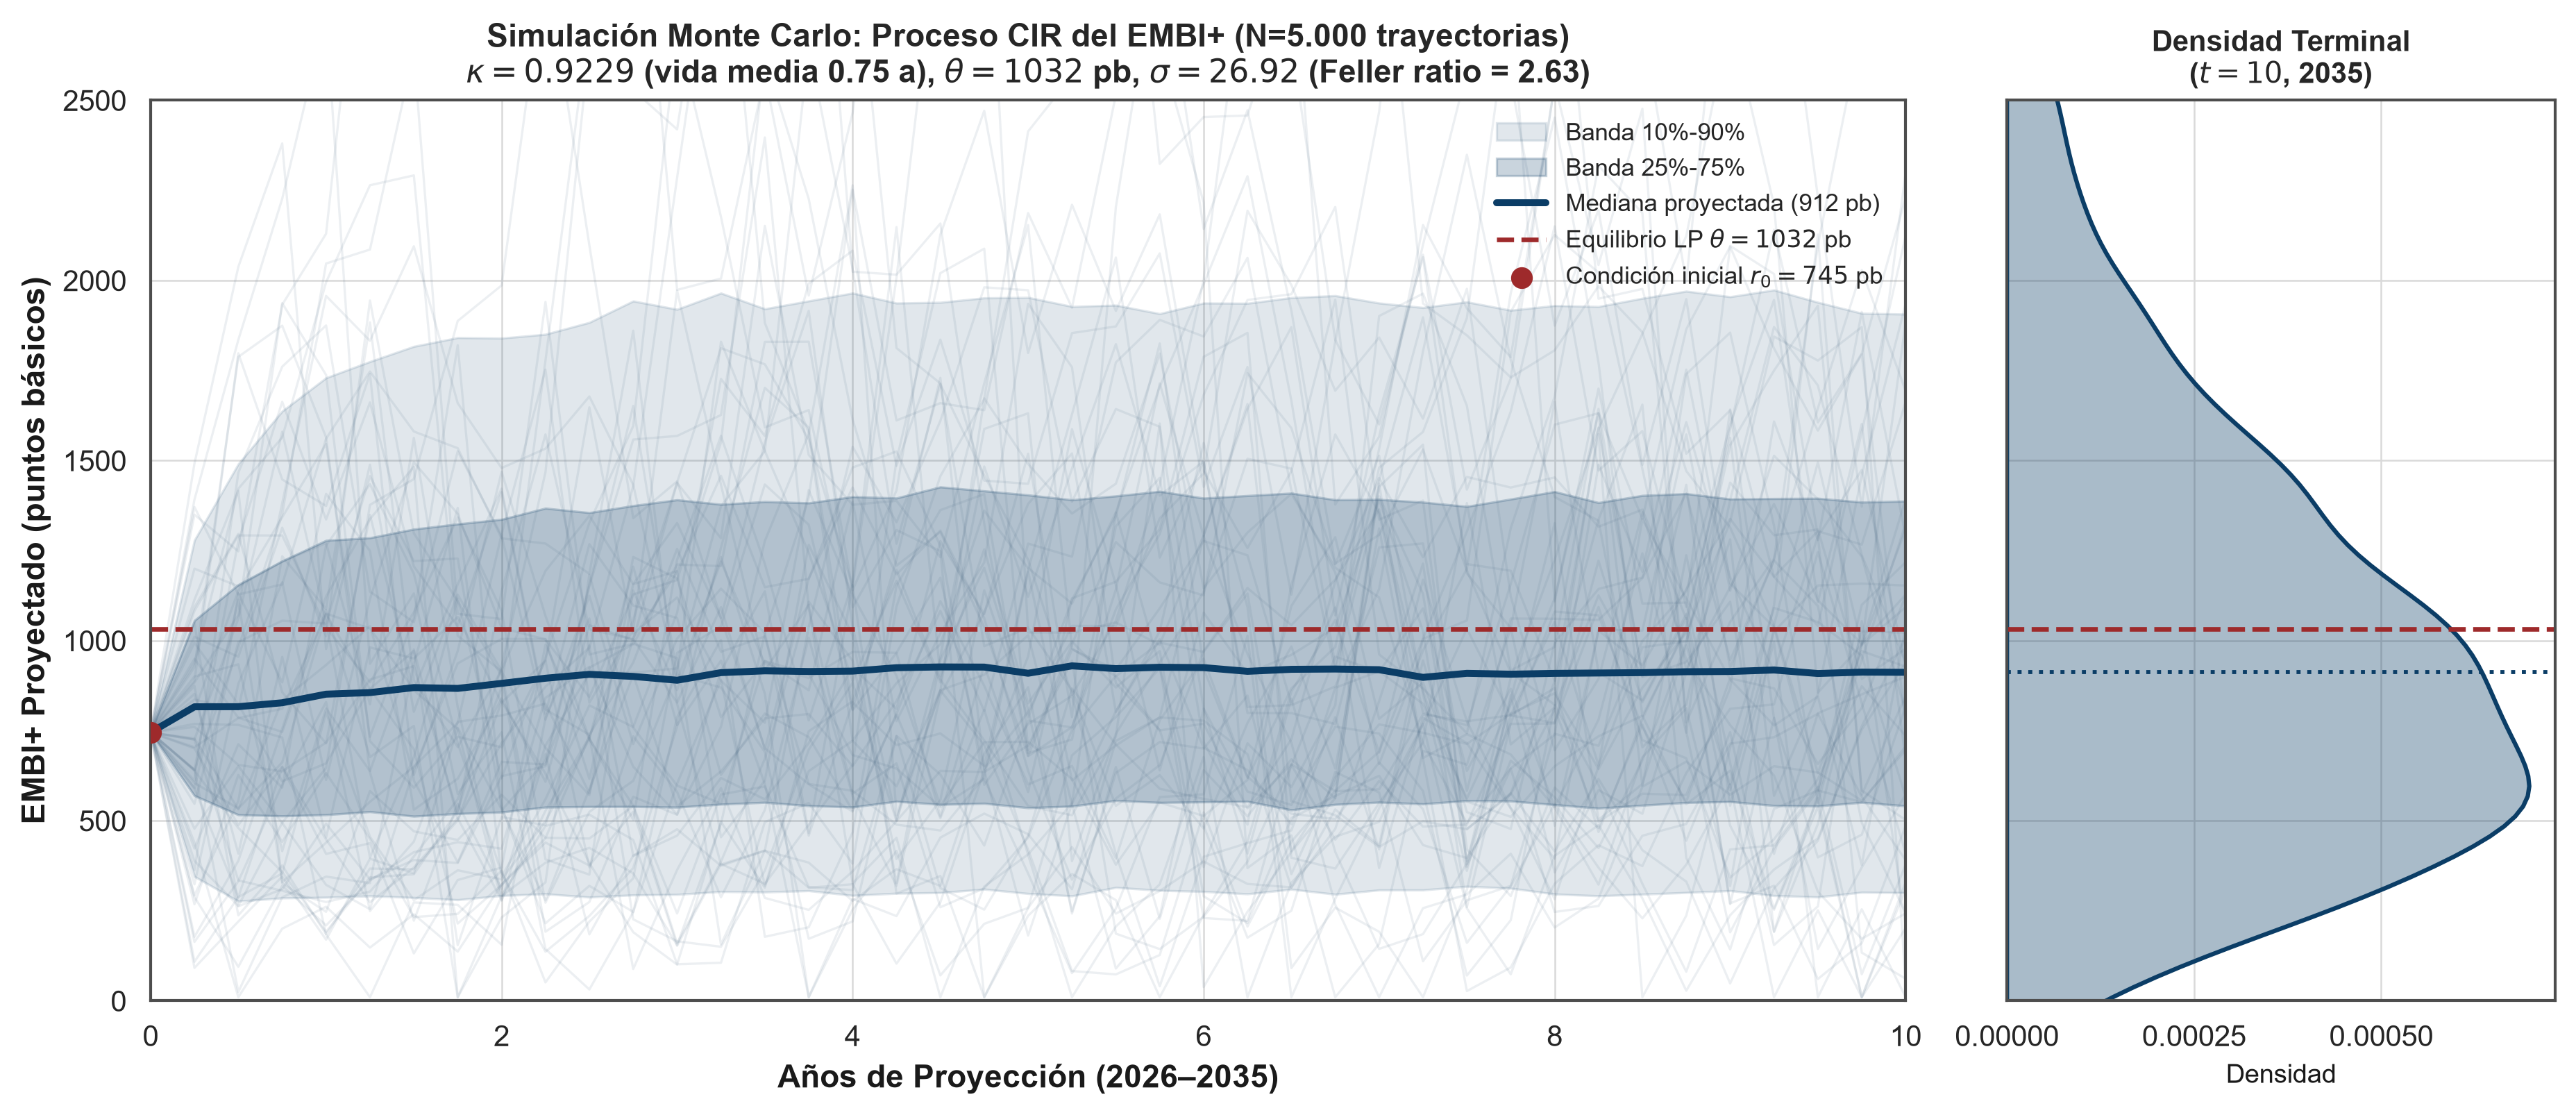
\includegraphics[width=0.92\textwidth]{figura_cir_simulacion.png}
\caption{Simulación Estocástica de Monte Carlo: Proceso CIR del EMBI+ y Densidad Terminal.}
\label{fig:cir_simulacion}
\end{figure}

Al integrar las 1.000 trayectorias continuas del proceso CIR en el módulo de proyección estocástica del DSA hacia 2035 (sustituyendo la tasa de refinanciación externa fija por $r_{f,t} = r_{US,t} + \text{CIR}_t$), la probabilidad estimada de insolvencia ($P(d_{2035} > 100\%)$) se sitúa en $\mathbf{29.8\%}$, convergiendo con gran consistencia con la cifra central de la calibración a mano que sostiene esta especificación alternativa ($31.2\%$) y sus robusteces ($30.4\%$ a $31.9\%$), y del mismo orden de magnitud que la especificación de referencia del cuerpo principal de la tesis, fundada en el SVAR ($26.1\%$, Sección \ref{sec:dsa_resultados} del Capítulo \ref{ch:resultados}).

\section{Estructura de la Cadena de Procesamiento de Código (Referencia)}
\label{sec:apendice_codigo}

La totalidad de los resultados cuantitativos reportados en esta tesis (estadísticas descriptivas, contrastes de raíz unitaria y cointegración, estimaciones DOLS/IV-2SLS/Hansen, quiebres de Bai-Perron, DCC-GARCH, deuda consolidada, diagnósticos de robustez de este Apéndice y simulaciones DSA) se computan mediante una cadena de procesamiento de código Python real y re-ejecutable, sin datos simulados ni resultados fabricados manualmente. Por razones de extensión, este Apéndice documenta la \textbf{estructura} de esa cadena de procesamiento y remite al archivo consolidado \texttt{codigo/codigo\_completo\_deuda.py}, que reúne el código fuente íntegro de cada etapa en un único documento de lectura, en lugar de reproducir aquí sus más de 4.100 líneas.

\footnotesize
\begin{longtable}{p{1.1cm}p{4.4cm}p{4.8cm}p{4.3cm}}
\caption{\label{tab:pipeline_estructura} Estructura de la Cadena de Procesamiento Empírico: Etapas, Scripts e Insumos/Salidas.} \\
\toprule
\textbf{Etapa} & \textbf{Script} & \textbf{Función} & \textbf{Salida} \\
\midrule
\endfirsthead
\multicolumn{4}{l}{\textit{Tabla A.3 (continuación)}} \\
\toprule
\textbf{Etapa} & \textbf{Script} & \textbf{Función} & \textbf{Salida} \\
\midrule
\endhead
\midrule
\multicolumn{4}{r}{\textit{Continúa en la página siguiente}} \\
\endfoot
\bottomrule
\endlastfoot
1.1--1.3 & \url{codigo/ingesta_datos/ingesta_datos_financieros.py} \newline \url{ingesta_bcra.py} \newline \url{ingesta_mecon_indec.py} & Descarga de series desde BCRA, MECON/INDEC (\url{datos.gob.ar}) y Yahoo Finance & Series brutas por fuente \\
1.4 & \url{codigo/ingesta_datos/construccion_dataset.py} & Orquesta 1.1--1.3, fusiona y valida el panel trimestral & \url{datos/dataset_consolidado_real.csv} ($n=88$) \\
1.5 & \url{ingesta_spread_regional.py} & Spread soberano regional (ETF EMB), Mejora Dim. III & \url{datos/procesados/spread_regional_trimestral.csv} \\
1.6 & \url{ingesta_bcra_pasivos.py} & Pasivos remunerados del BCRA (API v4.0), Mejora Dim. IV & \url{datos/procesados/bcra_pasivos_trimestral.csv} \\
2.1 & \url{codigo/modelos/fase1_estacionariedad.py} & Raíz unitaria (ADF, KPSS, PP, DF-GLS, Zivot-Andrews) & Tabla \ref{tab:estacionariedad}, Tabla \ref{tab:dfgls}, Sección \ref{sec:zivot_andrews} \\
2.2 & \url{fase2_cointegracion.py} & Cointegración de Johansen & Tabla de Johansen (Sección \ref{sec:johansen_cap6}) \\
2.3 & \url{fase3_reaccion_fiscal.py} & DOLS, diagnósticos de especificación & Tabla \ref{tab:dols} \\
2.4 & \url{fase4_variables_instrumentales.py} & IV-2SLS (VIX + spread regional), F de primera etapa, Wu-Hausman, Sargan & Tabla \ref{tab:iv2sls} \\
2.5 & \url{fase5_umbral_hansen.py} & Umbral de Hansen, \textit{bootstrap} Sup-LM & Tabla \ref{tab:hansen} \\
2.6 & \url{fase6_sostenibilidad_deuda.py} & DSA determinista y Monte Carlo (t de Student) & Tabla \ref{tab:dsa_determinista}, Figura \ref{fig:fan_chart_final} \\
2.7 & \url{fase7_diagnosticos_robustez.py} & ACF/PACF, ARCH-LM, CUSUM/CUSUMSQ, Engle-Granger, sensibilidad temporal, probabilidades por escenario, causalidad de Granger, filtro de Hamilton y covarianza del DSA vía GARCH(1,1) & Figuras \ref{fig:acf_pacf}, \ref{fig:cusum}; Tablas \ref{tab:sensibilidad_temporal}, \ref{tab:probabilidad_escenarios}, \ref{tab:engle_granger}, \ref{tab:garch_desvios}, \ref{tab:garch_dsa_comparacion} \\
2.8 & \url{fase8_deuda_consolidada.py} & Consolida deuda SPNF + pasivos BCRA, Mejora Dim. IV & Figura \ref{fig:deuda_consolidada}, Tabla \ref{tab:probabilidad_escenarios} (Sección \ref{sec:deuda_consolidada}) \\
2.9 & \url{bai_perron.py} \newline \url{fase9_bai_perron.py} & Quiebres estructurales múltiples (DP + BIC), Mejora Dim. I & Figura \ref{fig:bai_perron} (Sección \ref{sec:quiebres_estructurales}) \\
2.10 & \url{dcc_garch.py} \newline \url{fase10_dcc_garch.py} & DCC-GARCH, correlación condicional dinámica, Mejora Dim. II & Sección \ref{sec:dcc_garch} \\
2.11 & \url{fase11_dols_subperiodos.py} & DOLS por subperíodo ($m=1,2$) frente a MCO estático & Tabla \ref{tab:sensibilidad_temporal} (Sección \ref{sec:sensibilidad_temporal}) \\
2.12 & \url{fase12_diagnosticos_complementarios.py} & Selección del orden de rezagos del VAR (AIC/BIC/HQ/FPE), sensibilidad del rango de Johansen, VIF y número de condición & Tablas \ref{tab:rezagos_var} y \ref{tab:vif} \\
2.13 & \url{fase13_robustez_hansen_dpb.py} & Robustez del umbral de Hansen con $\Delta pb_t$ (I(0)) como dependiente & Tabla \ref{tab:hansen_dpb} (Sección \ref{sec:robustez_hansen_dpb}) \\
2.14 & \url{fase14_dsa_tail_dependence.py} & Robustez del DSA a la estructura de dependencia en colas (marginales $t$ independientes, cópula Gaussiana) & Tabla \ref{tab:tail_dependence_robustez} \\
2.15 & \url{fase15_sft_decomposicion_ilustrativa.py} & Descomposición ilustrativa del Ajuste Stock-Flujo ($SF_t$), episodios 2005/2018/2020 & Tabla \ref{tab:sft_ilustrativo} \\
2.16 & \url{fase16_vecm_dataset_ampliado.py} & Empalme histórico 1999--2003, estacionariedad, selección de rezagos del VAR, sensibilidad de Johansen al inicio muestral y estimación VECM sobre la ventana ampliada original ($n=108$); superado como fuente de las cifras de referencia por la Etapa 2.20 (ventana 1996--2025, $n=120$), se conserva en el repositorio por trazabilidad metodológica & --- \\
2.17 & \url{actualizar_tcrm_embi_real.py} & Reemplazo de las series de contingencia de TCRM y EMBI+ por series primarias (BCRA, Ámbito Financiero) en el panel consolidado & \url{datos/dataset_consolidado_real.csv} (actualizado) \\
2.18 & \url{fase17_calibracion_nu_dsa.py} & Recalibración de los grados de libertad $\nu$ de la $t$ de Student del DSA por método de momentos (curtosis), sobre \textit{shocks} reales & $\nu\approx4.8$ (Sección \ref{sec:aporte_metodologico}, Capítulo \ref{ch:discusion}) \\
2.19 & \url{fase18_dummies_presidenciales.py} & Robustez de $\alpha_{pb}$ por administración presidencial vía interacción con el término de corrección de error del VECM & Tabla \ref{tab:dummies_presidenciales} (Sección \ref{sec:dummies_presidenciales}) \\
2.20 & \url{codigo/ingesta_datos/construir_dataset_1996_2025.py} \newline \url{fase23_reestimacion_1996_2025.py} & Empalme histórico adicional 1996--1998, estacionariedad, Johansen (con sensibilidad al inicio muestral), estimación VECM (beta/alpha y sensibilidad de rezagos), SVAR restringido (FEVD) y TVECM sobre la ventana ampliada de treinta años ($n=120$), que reemplaza a la Etapa 2.16 como técnica de referencia; verificada además contra una corrida real sin aproximar el TCRM (ventana 1997--2025, $n=116$, salidas \texttt{fase23b\_*}) & Tabla \ref{tab:vecm_sensibilidad_inicio}, Tabla \ref{tab:vecm_beta_alpha}, Tabla \ref{tab:vecm_sensibilidad_lags}, Tabla \ref{tab:svar_fevd}, Tabla \ref{tab:tvecm} (Secciones \ref{sec:resultados_vecm}, \ref{sec:svar_resultados}, \ref{sec:tvecm_resultados}) \\
3.1--3.2 & \url{codigo/graficos/generacion_graficos_tesis.py} \newline \url{generacion_cronologia_quiebres.py} & Figuras 5.1, 5.3, 5.4 y 6.1 & Figuras del Capítulo \ref{ch:descriptivo} y \ref{ch:resultados} \\
\end{longtable}
\normalsize
\begin{flushleft}
\footnotesize \textit{Nota.} Todos los resultados intermedios se guardan adicionalmente en \texttt{resultados/tablas/*.csv} para trazabilidad. El archivo \texttt{codigo/codigo\_completo\_deuda.py} concatena el código fuente íntegro de las Etapas 1.1 a 3.2 en un único documento de lectura, indicando en cada sección la ruta del archivo original ejecutable. Los nombres de los scripts se corresponden uno a uno con las etapas del protocolo econométrico del Capítulo \ref{ch:metodologia}.
\end{flushleft}


\printbibliography

\end{document}
